% Generated by Sphinx.
\def\sphinxdocclass{report}
\documentclass[A4paperpaper,11pt,english]{sphinxmanual}
\usepackage[utf8]{inputenc}
\DeclareUnicodeCharacter{00A0}{\nobreakspace}
\usepackage{cmap}
\usepackage[T1]{fontenc}
\usepackage{babel}
\usepackage{times}
\usepackage[Bjarne]{fncychap}
\usepackage{longtable}
\usepackage{sphinx}
\usepackage{multirow}

\usepackage{pdfpages}
\setcounter{tocdepth}{2}
% \makeatletter
% \def\cleardoublepage{
% \clearpage\if@twoside \ifodd\c@page\else
% \hbox{}
% \vspace*{\fill}
% \vspace{\fill}
% \thispagestyle{empty}
% \newpage
% \if@twocolumn\hbox{}\newpage\fi\fi\fi
% }
% \makeatother

\renewcommand{\maketitle}{}


\title{Actin Gels dynamics}
\date{July 21, 2014 at 13:15:10 CEST}
\release{}
\author{Matthias Bussonnier}
\newcommand{\sphinxlogo}{}
\renewcommand{\releasename}{}
\makeindex

\makeatletter
\def\PYG@reset{\let\PYG@it=\relax \let\PYG@bf=\relax%
    \let\PYG@ul=\relax \let\PYG@tc=\relax%
    \let\PYG@bc=\relax \let\PYG@ff=\relax}
\def\PYG@tok#1{\csname PYG@tok@#1\endcsname}
\def\PYG@toks#1+{\ifx\relax#1\empty\else%
    \PYG@tok{#1}\expandafter\PYG@toks\fi}
\def\PYG@do#1{\PYG@bc{\PYG@tc{\PYG@ul{%
    \PYG@it{\PYG@bf{\PYG@ff{#1}}}}}}}
\def\PYG#1#2{\PYG@reset\PYG@toks#1+\relax+\PYG@do{#2}}

\expandafter\def\csname PYG@tok@gd\endcsname{\def\PYG@tc##1{\textcolor[rgb]{0.63,0.00,0.00}{##1}}}
\expandafter\def\csname PYG@tok@gu\endcsname{\let\PYG@bf=\textbf\def\PYG@tc##1{\textcolor[rgb]{0.50,0.00,0.50}{##1}}}
\expandafter\def\csname PYG@tok@gt\endcsname{\def\PYG@tc##1{\textcolor[rgb]{0.00,0.27,0.87}{##1}}}
\expandafter\def\csname PYG@tok@gs\endcsname{\let\PYG@bf=\textbf}
\expandafter\def\csname PYG@tok@gr\endcsname{\def\PYG@tc##1{\textcolor[rgb]{1.00,0.00,0.00}{##1}}}
\expandafter\def\csname PYG@tok@cm\endcsname{\let\PYG@it=\textit\def\PYG@tc##1{\textcolor[rgb]{0.25,0.50,0.56}{##1}}}
\expandafter\def\csname PYG@tok@vg\endcsname{\def\PYG@tc##1{\textcolor[rgb]{0.73,0.38,0.84}{##1}}}
\expandafter\def\csname PYG@tok@m\endcsname{\def\PYG@tc##1{\textcolor[rgb]{0.13,0.50,0.31}{##1}}}
\expandafter\def\csname PYG@tok@mh\endcsname{\def\PYG@tc##1{\textcolor[rgb]{0.13,0.50,0.31}{##1}}}
\expandafter\def\csname PYG@tok@cs\endcsname{\def\PYG@tc##1{\textcolor[rgb]{0.25,0.50,0.56}{##1}}\def\PYG@bc##1{\setlength{\fboxsep}{0pt}\colorbox[rgb]{1.00,0.94,0.94}{\strut ##1}}}
\expandafter\def\csname PYG@tok@ge\endcsname{\let\PYG@it=\textit}
\expandafter\def\csname PYG@tok@vc\endcsname{\def\PYG@tc##1{\textcolor[rgb]{0.73,0.38,0.84}{##1}}}
\expandafter\def\csname PYG@tok@il\endcsname{\def\PYG@tc##1{\textcolor[rgb]{0.13,0.50,0.31}{##1}}}
\expandafter\def\csname PYG@tok@go\endcsname{\def\PYG@tc##1{\textcolor[rgb]{0.20,0.20,0.20}{##1}}}
\expandafter\def\csname PYG@tok@cp\endcsname{\def\PYG@tc##1{\textcolor[rgb]{0.00,0.44,0.13}{##1}}}
\expandafter\def\csname PYG@tok@gi\endcsname{\def\PYG@tc##1{\textcolor[rgb]{0.00,0.63,0.00}{##1}}}
\expandafter\def\csname PYG@tok@gh\endcsname{\let\PYG@bf=\textbf\def\PYG@tc##1{\textcolor[rgb]{0.00,0.00,0.50}{##1}}}
\expandafter\def\csname PYG@tok@ni\endcsname{\let\PYG@bf=\textbf\def\PYG@tc##1{\textcolor[rgb]{0.84,0.33,0.22}{##1}}}
\expandafter\def\csname PYG@tok@nl\endcsname{\let\PYG@bf=\textbf\def\PYG@tc##1{\textcolor[rgb]{0.00,0.13,0.44}{##1}}}
\expandafter\def\csname PYG@tok@nn\endcsname{\let\PYG@bf=\textbf\def\PYG@tc##1{\textcolor[rgb]{0.05,0.52,0.71}{##1}}}
\expandafter\def\csname PYG@tok@no\endcsname{\def\PYG@tc##1{\textcolor[rgb]{0.38,0.68,0.84}{##1}}}
\expandafter\def\csname PYG@tok@na\endcsname{\def\PYG@tc##1{\textcolor[rgb]{0.25,0.44,0.63}{##1}}}
\expandafter\def\csname PYG@tok@nb\endcsname{\def\PYG@tc##1{\textcolor[rgb]{0.00,0.44,0.13}{##1}}}
\expandafter\def\csname PYG@tok@nc\endcsname{\let\PYG@bf=\textbf\def\PYG@tc##1{\textcolor[rgb]{0.05,0.52,0.71}{##1}}}
\expandafter\def\csname PYG@tok@nd\endcsname{\let\PYG@bf=\textbf\def\PYG@tc##1{\textcolor[rgb]{0.33,0.33,0.33}{##1}}}
\expandafter\def\csname PYG@tok@ne\endcsname{\def\PYG@tc##1{\textcolor[rgb]{0.00,0.44,0.13}{##1}}}
\expandafter\def\csname PYG@tok@nf\endcsname{\def\PYG@tc##1{\textcolor[rgb]{0.02,0.16,0.49}{##1}}}
\expandafter\def\csname PYG@tok@si\endcsname{\let\PYG@it=\textit\def\PYG@tc##1{\textcolor[rgb]{0.44,0.63,0.82}{##1}}}
\expandafter\def\csname PYG@tok@s2\endcsname{\def\PYG@tc##1{\textcolor[rgb]{0.25,0.44,0.63}{##1}}}
\expandafter\def\csname PYG@tok@vi\endcsname{\def\PYG@tc##1{\textcolor[rgb]{0.73,0.38,0.84}{##1}}}
\expandafter\def\csname PYG@tok@nt\endcsname{\let\PYG@bf=\textbf\def\PYG@tc##1{\textcolor[rgb]{0.02,0.16,0.45}{##1}}}
\expandafter\def\csname PYG@tok@nv\endcsname{\def\PYG@tc##1{\textcolor[rgb]{0.73,0.38,0.84}{##1}}}
\expandafter\def\csname PYG@tok@s1\endcsname{\def\PYG@tc##1{\textcolor[rgb]{0.25,0.44,0.63}{##1}}}
\expandafter\def\csname PYG@tok@gp\endcsname{\let\PYG@bf=\textbf\def\PYG@tc##1{\textcolor[rgb]{0.78,0.36,0.04}{##1}}}
\expandafter\def\csname PYG@tok@sh\endcsname{\def\PYG@tc##1{\textcolor[rgb]{0.25,0.44,0.63}{##1}}}
\expandafter\def\csname PYG@tok@ow\endcsname{\let\PYG@bf=\textbf\def\PYG@tc##1{\textcolor[rgb]{0.00,0.44,0.13}{##1}}}
\expandafter\def\csname PYG@tok@sx\endcsname{\def\PYG@tc##1{\textcolor[rgb]{0.78,0.36,0.04}{##1}}}
\expandafter\def\csname PYG@tok@bp\endcsname{\def\PYG@tc##1{\textcolor[rgb]{0.00,0.44,0.13}{##1}}}
\expandafter\def\csname PYG@tok@c1\endcsname{\let\PYG@it=\textit\def\PYG@tc##1{\textcolor[rgb]{0.25,0.50,0.56}{##1}}}
\expandafter\def\csname PYG@tok@kc\endcsname{\let\PYG@bf=\textbf\def\PYG@tc##1{\textcolor[rgb]{0.00,0.44,0.13}{##1}}}
\expandafter\def\csname PYG@tok@c\endcsname{\let\PYG@it=\textit\def\PYG@tc##1{\textcolor[rgb]{0.25,0.50,0.56}{##1}}}
\expandafter\def\csname PYG@tok@mf\endcsname{\def\PYG@tc##1{\textcolor[rgb]{0.13,0.50,0.31}{##1}}}
\expandafter\def\csname PYG@tok@err\endcsname{\def\PYG@bc##1{\setlength{\fboxsep}{0pt}\fcolorbox[rgb]{1.00,0.00,0.00}{1,1,1}{\strut ##1}}}
\expandafter\def\csname PYG@tok@kd\endcsname{\let\PYG@bf=\textbf\def\PYG@tc##1{\textcolor[rgb]{0.00,0.44,0.13}{##1}}}
\expandafter\def\csname PYG@tok@ss\endcsname{\def\PYG@tc##1{\textcolor[rgb]{0.32,0.47,0.09}{##1}}}
\expandafter\def\csname PYG@tok@sr\endcsname{\def\PYG@tc##1{\textcolor[rgb]{0.14,0.33,0.53}{##1}}}
\expandafter\def\csname PYG@tok@mo\endcsname{\def\PYG@tc##1{\textcolor[rgb]{0.13,0.50,0.31}{##1}}}
\expandafter\def\csname PYG@tok@mi\endcsname{\def\PYG@tc##1{\textcolor[rgb]{0.13,0.50,0.31}{##1}}}
\expandafter\def\csname PYG@tok@kn\endcsname{\let\PYG@bf=\textbf\def\PYG@tc##1{\textcolor[rgb]{0.00,0.44,0.13}{##1}}}
\expandafter\def\csname PYG@tok@o\endcsname{\def\PYG@tc##1{\textcolor[rgb]{0.40,0.40,0.40}{##1}}}
\expandafter\def\csname PYG@tok@kr\endcsname{\let\PYG@bf=\textbf\def\PYG@tc##1{\textcolor[rgb]{0.00,0.44,0.13}{##1}}}
\expandafter\def\csname PYG@tok@s\endcsname{\def\PYG@tc##1{\textcolor[rgb]{0.25,0.44,0.63}{##1}}}
\expandafter\def\csname PYG@tok@kp\endcsname{\def\PYG@tc##1{\textcolor[rgb]{0.00,0.44,0.13}{##1}}}
\expandafter\def\csname PYG@tok@w\endcsname{\def\PYG@tc##1{\textcolor[rgb]{0.73,0.73,0.73}{##1}}}
\expandafter\def\csname PYG@tok@kt\endcsname{\def\PYG@tc##1{\textcolor[rgb]{0.56,0.13,0.00}{##1}}}
\expandafter\def\csname PYG@tok@sc\endcsname{\def\PYG@tc##1{\textcolor[rgb]{0.25,0.44,0.63}{##1}}}
\expandafter\def\csname PYG@tok@sb\endcsname{\def\PYG@tc##1{\textcolor[rgb]{0.25,0.44,0.63}{##1}}}
\expandafter\def\csname PYG@tok@k\endcsname{\let\PYG@bf=\textbf\def\PYG@tc##1{\textcolor[rgb]{0.00,0.44,0.13}{##1}}}
\expandafter\def\csname PYG@tok@se\endcsname{\let\PYG@bf=\textbf\def\PYG@tc##1{\textcolor[rgb]{0.25,0.44,0.63}{##1}}}
\expandafter\def\csname PYG@tok@sd\endcsname{\let\PYG@it=\textit\def\PYG@tc##1{\textcolor[rgb]{0.25,0.44,0.63}{##1}}}

\def\PYGZbs{\char`\\}
\def\PYGZus{\char`\_}
\def\PYGZob{\char`\{}
\def\PYGZcb{\char`\}}
\def\PYGZca{\char`\^}
\def\PYGZam{\char`\&}
\def\PYGZlt{\char`\<}
\def\PYGZgt{\char`\>}
\def\PYGZsh{\char`\#}
\def\PYGZpc{\char`\%}
\def\PYGZdl{\char`\$}
\def\PYGZhy{\char`\-}
\def\PYGZsq{\char`\'}
\def\PYGZdq{\char`\"}
\def\PYGZti{\char`\~}
% for compatibility with earlier versions
\def\PYGZat{@}
\def\PYGZlb{[}
\def\PYGZrb{]}
\makeatother

\begin{document}

\maketitle
%%       \begin{center}
%%        \begin{minipage}{0.75\linewidth}
%%            \centering
%%            % \rule{0.4\linewidth}{0.15\linewidth}\par
%%            {\uppercase{\large \'Ecole Doctorale Mati\`ere Condend\'ee et interface \par}}
%%            {\uppercase{\large Laboratoire Physique Chimie du Vivant, Institut Curie, Umr 168 \par}}
%%            \vspace{2cm}
%%            {\uppercase{\Large  Doctorat \par}}
%%            {\uppercase{\Large  Physique \par}}
%%            \vspace{2cm}
%%           {\Large Bussonnier Matthias\par}
%%            \vspace{2cm}
%%            {\Large Actin Gel mechanics\par}
%%            {\Large Mechanique des gels d'actine\par}
%%            \vspace{2cm}
%%            \Large
%%            Th\`ese diri\'ee par Timo Betz et C\'ecile Sykes,\\
%%            Soutenue le 16 Septembre 2014\\
%%            \vspace{2cm}
%%                {\Large Jury}
%%            \vspace{1cm}
%%                \large
%%                \begin{flushleft}
%%                Prof. Atef Anacios , Pr\'esident\\
%%                Dr. Laurent Blanchoin\\
%%                Dr. Guillaume Rommet-Lemonne, Rapporteur\\
%%                Prof. Dr. Dr. Karsten Kruse, Rapporteur\\
%%                \end{flushleft}
%%
%%            \vspace{2cm}
%%        \end{minipage}
%%    \end{center}
%%    \newpage

    \begin{center}
        \begin{minipage}{0.75\linewidth}
    \begin{center}
            \noindent {\large \textbf{UNIVERSITÉ PARIS DIDEROT - SORBONNE PARIS CITÉ}} \\ 
            \vspace*{0.3cm}
            \noindent {\large \textbf{ÉCOLE DOCTORALE 518}} \\
            \noindent \textbf{CONDENSED MATTER \\ AND INTERFACES} \\
            \vspace*{0.5cm}
            \noindent \Huge \textbf{T H È S E} \\
            \vspace*{0.3cm}
            \noindent \large {pour obtenir le grade de} \\
            \vspace*{0.3cm}
            \noindent \LARGE \textbf{Docteur en Sciences} \\
            \vspace*{0.3cm}
            \noindent \Large de l'Université PARIS DIDEROT (Paris 7) \\
            %\noindent \Large \textbf{Spécialité : \textsc{Interface Physique-Biologie}}\\
            \vspace*{0.4cm}
            \noindent \large {Présentée et soutenue par\\}
            \noindent \LARGE Matthias \textsc{Bussonnier} \\
            \vspace*{0.8cm}
            \noindent {\Huge \textbf{Actin Gel mechanics \\ Mécanique des Gels D'actine}} \\
            \vspace*{0.8cm}
            \noindent \Large Thèse dirigée par Timo \textsc{Betz} et Cécile \textsc{Sykes} \\
            \vspace*{0.2cm}
            \noindent \Large préparée à l'Institut Curie \\
            \vspace*{0.2cm}
            \noindent \large Soutenance le 16 Septembre 2014, devant le jury composé de~:\\
            \vspace*{0.5cm}
            \end{center}
            %\noindent \large \textbf{Jury :} \\
            \begin{center}
            \noindent \large 
            \begin{tabular}{llcl}
                \textit{Président :}    & Prof. Atef            \textsc{Asnacios }       & - & Université Paris Diderot \\
                \textit{Rapporteurs :}  & Prof. Dr. Dr. Karsten \textsc{Kruse}           & - & Universität des Saarlandes \\
                                        & Dr. Guillaume         \textsc{Romet-Lemonne}   & - & LEBS - CNRS\\
                            
                \textit{Examinateurs :} & Dr. Laurent           \textsc{Blanchoin}       & - & CEA Grenoble\\
                \textit{Directeurs : }  & Dr. Timo              \textsc{Betz}            & - & Institut Curie\\
                                        & Prof. Cécile          \textsc{Sykes}           & - & Institut Curie\\
                            
            \end{tabular}
            \end{center}
        \end{minipage}
    \end{center}
    \clearpage
    \null
    \thispagestyle{empty}%
    \addtocounter{page}{-1}%
    \newpage


% \\pagestyle{frontmatter}
% \\chapter*{Abstract}
% \\thispagestyle{frontmatter}
% %s
% \\chapter*{Foreword}
% \\thispagestyle{frontmatter}
% %s
% \\chapter*{Acknowledgements}
% \\thispagestyle{frontmatter}
% --s
\tableofcontents
% \\cleardoublepage
% \\pagestyle{frontmatter}
% \\addtocontents{toc}{\\protect\\thispagestyle{frontmatter}}
% \\listoffigures
% \\addtocontents{lof}{\\protect\\thispagestyle{frontmatter}}
% \\listoftables
% \\addtocontents{lot}{\\protect\\thispagestyle{frontmatter}}
\cleardoublepage
\pagestyle{normal}
\pagenumbering{arabic}
\setlength{\headheight}{14pt}
 
\phantomsection\label{index-latex::doc}



\chapter*{Preamble}
\label{index-latex:preamble}\label{index-latex::doc}\label{index-latex:contents}
During my PhD I decided to investigate the effect of the actin network on the
mechanical properties of cells. Indeed, cell mechanics are a key parameter that
has crucial impact on cellular and organisms functions. Being able to detect
changes in the mechanical properties, and to understand the mechanism that
govern these changes  is an important step in the study of cellular behavior as
well as in differentiating healthy from cancerous cells and tissue.
Understanding the mechanisms that are at the origin of cell motion and shape
changes is also a decisive step in controlling cell behavior, with the ultimate
goal to prevent cancer cell invasion and division without impairing healthy
cells.

During the last three years, I decided to focus on biomimetic system and
to determine the characteristics of actin networks. Actin is a highly conserved
component across the living domain, and it plays a major role in cell
mechanics. By interacting with a number of other components of the cell, actin
is able to form various different types of networks. I decided to focus my research on such networks that were created under
controlled conditions.

Along this dissertation we will mainly focus on three systems.

First, we reconstitute an already observed actin network — the actin
cortex — on a biomimetic system, then show that a
second sparse actin network that was previously unseen emanates from it, and finally characterize its mechanical
properties. We developed the idea that the effect of this second network cannot
be neglected in cells and investigate a few of the phenomenon it may be involved
in.

As the effect of such a sparse actin has not been demonstrated in living cells, we decided to
investigate the effect of another sparse actin network found in a living cells. In
collaboration with the group of Marie Hélène Verlhac at College de France, we studied the mechanical properties
in the cytosol of mouse oocytes. We see in this system that actin related proteins have
hi-impact on the structure and the mechanics of both the cell and the actin
network.

Characterizing the dynamics of a network in a living cell by controlling the
conditions remains complex.  In a third research stream we characterized the dynamical changes of tension created by reconstituted actin
cortices that are linked to a lipid
membrane. By studying liposome ``doublets'' we are able to measure the variation of tension generated by the acto-myosin cortex over
time. This system is composed by a liposome doublet covered with
an actin network. Imaging with Spinning disk microscopy, we are able to
reconstruct changes in the acto-myosin network and deduce the changes in its
properties from the geometrical variation during network contraction.


\chapter{Background}
\label{index-latex:background}

\section{Introduction}
\label{index-latex:introduction}
Cells are the basic components of living organisms. Understanding their
individual behavior and the way they function is a key step to understand
how they interact with their environment. One of the key components within most
cells is the actin cytoskeleton, which is made up of actin monomers, a protein that is highly conserved across species and which plays
an important role for cell mechanics, ranging from cell migration to cell differentiation
and division. It plays hence a crucial role for the mechanical properties of
the cell and its mechanical interaction with the environment. Under the cell membrane lies a
thin actin network which controls the mechanical properties of the cell:
the actin cortex. The mechanical behavior of this actin cortex is itself driven
by the dynamics and interaction within the actin network it is made off.
Understanding this actin network is hence a key to learn how the actin
cortex behaves, leading to a better understanding of cells and tissue.

The properties of an actin network highly depend on its structure. The
structure itself depends on many parameters that influence how the network is
formed.  The network structure and formation is influenced by physical and
chemical conditions and the spatial and temporal variation of these parameters like mechanical
stress or ion-concentration can determine the fate of the network. Hence it is
important to study these networks and their dynamic behaviour in order to grasp the
changing structure of the cell.

Cells are complex systems that adapt their shape, mechanical properties and
biochemical conditions permanently. The spatial repartition of theses
properties is also variable as the cell regulates the concentration of proteins
all across its cytoplasm. To well study the effect of each component independently,
it is crucial to study actin networks in a controlled environment.

Biomimetic systems allow to respond to most of these concerns, they provide a
controlled environment that mimic \emph{in-vivo} phenomena. Biochemical conditions
can be well controlled, both in space and time hence allowing to precisely fine tune
experimental conditions. Biomimetic systems are also particularly adapted to be combined with
optical traps which allow us to study local mechanical properties of actin
networks with high temporal resolution. The combination of both allows us to get
insight into the variation of theses mechanical properties as a function of
time and space with high precision.

During my PhD, I have focused on the mechanical properties of branched actin
networks polymerizing on optically trapped polystyrene beads. Such networks where
studied before {\hyperref[index-latex:kawska2012]{{[}Kawska, Carvalho, Manzi,  et al.  2012{]}}} but have been suspected to be highly
inhomogeneous. Optical traps allows to probe the mechanics of yet unaccessible parts of
the network.
I further studied actin
networks on other biomimetic systems constituted of liposomes, in order to better
understand the effect of actin cortex polymerisation on membrane tension and to
characterize network dynamics over time. Finally,  I participated in a
collaboration in order to understand the implication such actin networks in
living mouse oocytes.


\section{Living Cells}
\label{index-latex:living-cells}
Cells are the basic building blocks of life, and all living beings are composed of
cells, from unicellular up to multicellular organisms like us. Unicellular
organisms must accomplish all their functions within a single cell. At the other end,
in multicellular organisms cells differentiate in order to accomplish specialised
tasks often by regrouping into organs. Despite sharing the same genetic
material, for each cell to accomplish a different task often requires different
mechanical properties. The variation of elasticity and other
mechanical properties of cells derive from the structure they are composed of.

Cells are hence able to adapt to their environment and develop functions and
behavior that may change over time. A small change of timing and/or biochemical
conditions can highly injure the development of an organism: for example modification of
the actin network at a given time during the cell cycle prevents symmetric division
{\hyperref[index-latex:lenart2005]{{[}Lenart, Bacher, Daigle,  et al.  2005{]}}}, {\hyperref[index-latex:vasilev2012]{{[}Vasilev, Chun, Gragnaniello,  et al.  2012{]}}}. Furthermore, the mechanical properties of the substrate can
govern the differentiation of cells: Soft substrate will favor brain-tissue
cell, where stiff substrates increase the appearance of muscle cells
{\hyperref[index-latex:engler2006]{{[}Engler, Sen, Sweeney, Discher,  2006{]}}}.

Nonetheless, even with all theses different behavior and phenotypes, cells
have a common structure. The exterior of the cell is separated from the
inside by a plasma membrane. The interior of the cell is filled with the cytoplasm
which contains diverse structures such as organelles, genetic material, and
a large number of proteins that the cell uses to accomplish its functions. To
communicate with the outside, cells have a series of mechanisms that allow signals
and cargo to pass the membrane. This communication can be chemical, but
mechanics is also known to participate in the process. To sense their
mechanical environment, cells often use adhesion complexes to attach to the
substrate, and integrins as trans-membrane protein to transfer the force to the
cell cytoskeleton situated inside the cell. Chemical signals can either cross
the membrane through trans-membrane proteins, while endocytosis and exocytosis are
ways for the cell to import and export proteins and chemicals through its membrane.


\section{Oocyte}
\label{index-latex:oocyte}
A particular cell type I was interested in during my PhD are mouse oocytes.
Oocytes are female germinal cells in the process of gametogenesis. Unlike
somatic cells that undergoes symmetric division via mitosis which leads to
two identical cells sharing the same genetic material, oocytes undergo a
different process called meiosis.  Meiosis in oocytes is a highly asymmetric
process necessary for the specificity of being large haploid
cells, containing at the end of meiosis only one chromosome of each pair
that constitutes the genetic material of a mouse. The second chromosome of each pair
will be provided during fertilisation of the oocyte by the male sperm.

The exact process of oocyte formation can vary among species, and in the following we will
describe the main mechanisms.

The complete process of egg maturation starts with primordial germ cells that
undergo mitosis to replicate until they enter the first meiosis (Meiosis I)
at which state they are called primary oocytes and are still diploid, that is to say still contains two chromosomes of each pair.

The primary oocyte will start maturation and growth and then undergo a first
asymmetric division just after prophase I.  This first division is asymmetric
both in the genetic material separation and in the unequal size of the formed
daughter cell. Indeed, the primary oocyte will divide into a secondary oocyte
and a polar body. Both, the secondary oocyte and the polar body are haploid and contain
only half of the genetic material of the primary oocyte.  The secondary oocyte
can go through Meiosis II in which it undergoes a second asymmetric division
and expulsion of a second polar body. These polar bodies will eventually degenerate
(\hyperref[index-latex:fig-asymetric-division]{Fig  \ref*{index-latex:fig-asymetric-division}}).

During meiosis, the process of cell division also differ from mitosis. Instead
of separating into two identically sized cells through the formation of a
cytokinetic ring, the primary oocyte will become the secondary oocyte by
expulsion a polar body. The formation expulsion of the polar body require
precise positioning of the cell organelles. During prophase I the nucleus of
the oocyte is carefully centered, undergoes a nuclear breakdown and spindle formation.
The first meiotic spindle will migrate toward the oocyte cortex along
its major axis. Once at the cortex, half of the genetic material of the spindle
will be expelled through the membrane forming the first polar body of much
smaller size than second oocyte.

Mouse oocyte are good model systems to study the mechanical properties inside
cells. They form big spherical cells with a diameter of around 80 µm
which allow to study the mechanical properties at different locations in
the cytoplasm.

In the third part of my PhD I participated in a collaboration with Marie-Hélène
Verlhac and Maria Almonacid at Collège de France who are interested in the
effect of actin dynamics in oocyte cytoplasm during the different parts of
oocyte gametogenesis.
\begin{figure}[htbp]
\centering
\capstart

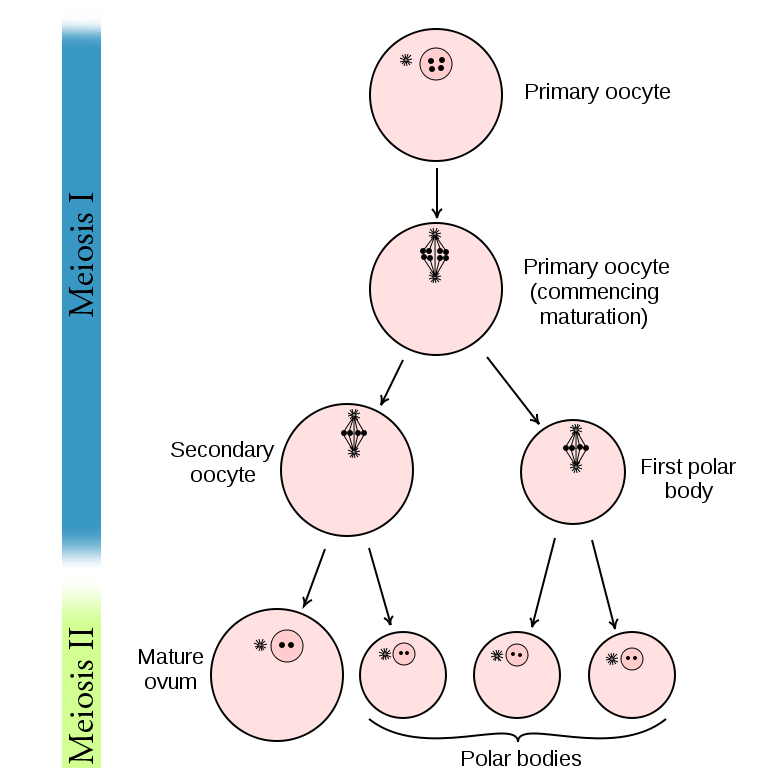
\includegraphics[width=0.800\linewidth]{oocyte-polar.png}
\caption{Asymmetric division of oocytes into polar bodies. The primary oocyte
asymmetrically divide into a secondary oocyte and a smaller polar body each
containing half the DNA of the mother cell. The secondary oocyte will
divide asymmetrically a second time to become the mature ovum while
expelling a polar body. This asymmetric division process allow the
formation of a large haploid cell. Adapted from Wikipedia – Gray's
Anatomy – and {\hyperref[index-latex:alberts2008]{{[}Alberts, Johnson, Lewis,  et al.  2008{]}}}.}\label{index-latex:fig-asymetric-division}\end{figure}


\subsection{Cell Organelles}
\label{index-latex:cell-organelles}
Inside the cytoplasm, cells have a number of structures with different and
specialised functions which are called organelles. The position and state of
organelles is of great importance for the cell to achieve its functions.
Probably the most known organelle is the cell nucleus of eukariotic cells that
contains the genetic material. Attached to the nucleus is the endoplasmic
reticulum  which is the organelle responsible for translating
RNA coming from the nucleus to functional proteins that will be delivered
across the cell after maturation in vesicles. Theses vesicles are
transported across the cell both by dyneins and kinesins — molecular motors —
that walk along microtubules originating from the centriole part of the
centrosome but also by myosins walking along actin filaments.  All of those processes
consume energy in  the form of ATP, generated within the mitocondria spread
across the cytoplasm. A schematic of the cell with some organelles can be seen
on \hyperref[index-latex:albertcell]{figure  \ref*{index-latex:albertcell}}
\begin{figure}[htbp]
\centering
\capstart

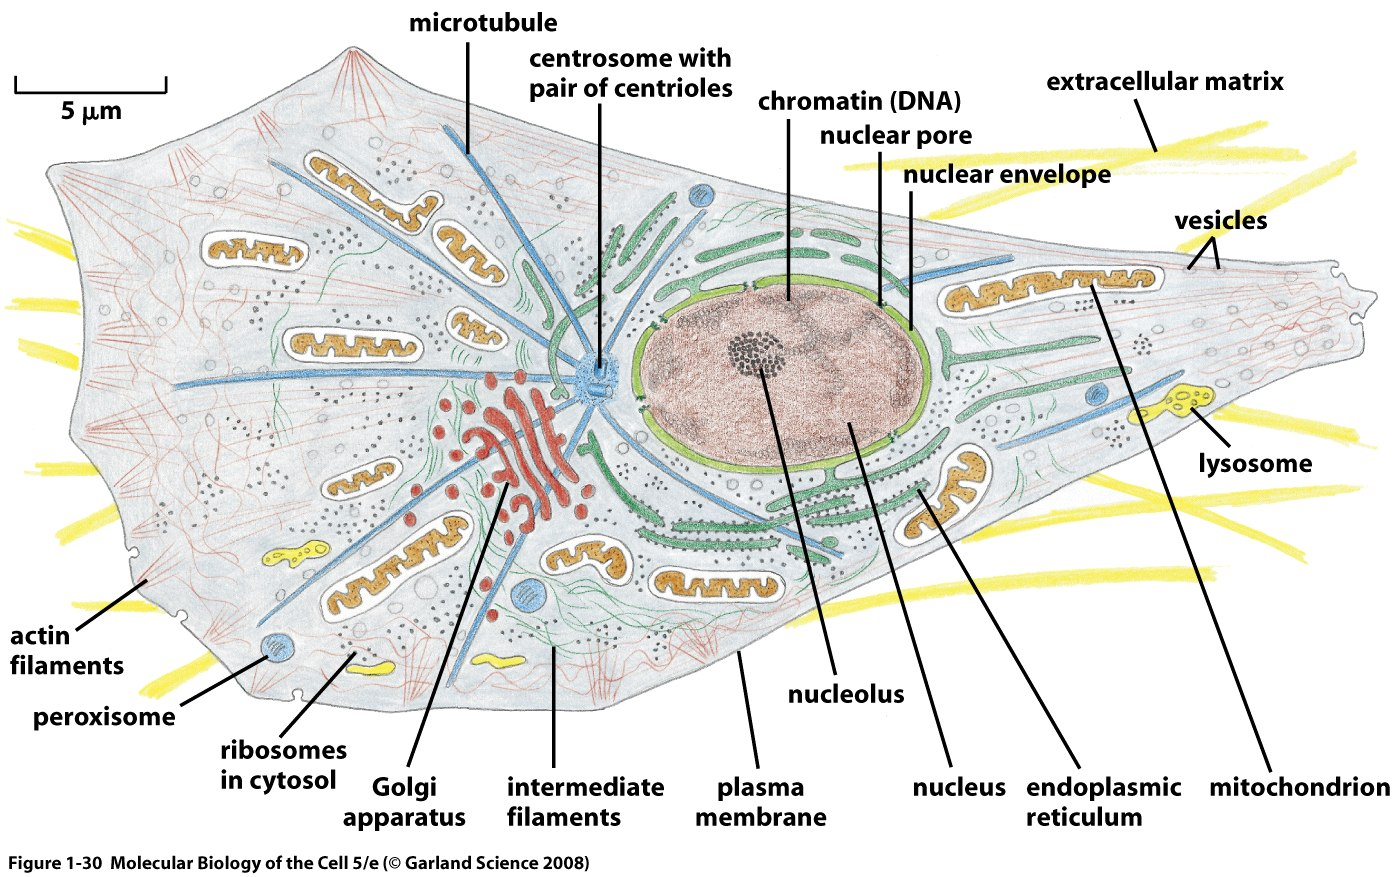
\includegraphics[width=0.800\linewidth]{figure-1-30.jpg}
\caption{Schematic of an eukariotic cell, adapted from {\hyperref[index-latex:alberts2008]{{[}Alberts, Johnson, Lewis,  et al.  2008{]}}}. Visualized are
the many components that constitute the majority of cells.  Cell shape and
size can highly vary, from quasi spherical with a typical size of ten
micrometers to elongated neurones that can be tens of centimeters long.}\label{index-latex:albertcell}\end{figure}

The positioning of organelles is crucial for the life of the cell. During
meiotic division of cells, for example, it has been seen that the positioning of
the nucleus at the center of mouse oocytes happens before its
migration closer to the cortex to expel the first polar body. Failure to do so
results in a incorrect amount of DNA in germinal cell that can lead to
infertility.

It is already known that microtubules play a key role in organelle positioning.
Microtubules emanating from centrosome position at the two ends of the cell
during its division are used to fetch the correct chromosomes. Each
chromosome is pulled towards the centrosome which leads to each daughter
cell having the same amount of DNA.

Actin plays also an determinant role in organelle positioning process,
like in drosophila oocyte maturation where it positions the nurses cell away
from the dumping canal {\hyperref[index-latex:huelsmann2013]{{[}Huelsmann, Ylanne, Brown,  2013{]}}}. In a later chapter ({\hyperref[index-latex:organelle-positioning]{\emph{Organelle
Positioning}}} (\autopageref*{index-latex:organelle-positioning})) we will develop a few keys points where
actin is indispensable in organelle positioning and how this relate to the
biomimetic actin networks we reconstitute.


\subsection{The Cytoskeleton}
\label{index-latex:intro-cyto}\label{index-latex:the-cytoskeleton}
The cytoskeleton, literally skeleton of the cell, is the structure which gives
the shape to a cell.  As for other multicellular animals that posses
skeleton, its shape is often a hint on how an organism moves. As feet, fins and
wings are characteristics that will tell you whether a animal
prefer land, see or air, the cytoskeleton will tell you many
things about a cell.

Unlike the (exo)-skeleton of animals which is rigid and
static, the cytoskeleton of cell is a  highly dynamic structure that keeps
remodeling itself on a short time scale compared to the speed at which a cells
move. Thanks to these dynamics, the cytoskeleton can achieve its
functions.  As vertebrates skeletons are necessary to transmit force from one part
of the body to another, the cytoskeleton is responsible not only to
transmit the forces the cell is exerting, but also to generate theses forces.
The cytoskeleton connect a cell to its environment,
both mechanically and biochemically.

We will consecrate a longer part of this work to describe the cytoskeleton.


\section{The Role And Composition Of The Cytoskeleton}
\label{index-latex:the-role-and-composition-of-the-cytoskeleton}\label{index-latex:role-of-actin}
We have already introduced the cell cytoskeleton in the previous part, and we will now
describe its components and functionality more in detail here.  The cytoskeleton
has three main functions, it connects the cell both physically
and biochemically to the external environment, generate and coordinate the
forces that give the cell its shape and allows it to move. It is also
responsible for organising spatially  the cell content {\hyperref[index-latex:fletcher2010]{{[}Fletcher, Mullins,  2010{]}}}.
The cytoskeleton is also in particular sensitive to spatial and temporal
information that can affect cell fate and the assembly of the cytoskeletal
structure. This can be seen for example with the bud scar of budding yeast that
persists after division.


\subsection{Composition of the cell cytoskeleton}
\label{index-latex:composition-of-the-cell-cytoskeleton}
The cytoskeleton is mainly composed of three types of filaments.
Microtubules, intermediate filament and actin filament, also known as
microfilaments.

Microtubules are the widest structure with a diameter of 20nm (\hyperref[index-latex:fig-mt]{Fig  \ref*{index-latex:fig-mt}})
and the
stiffest of the three kinds of filaments with a {\hyperref[index-latex:viscoelastic]{\emph{persistence length}}} (\autopageref*{index-latex:viscoelastic}) in the order
of millimeters, much longer than the size of the usual cell.
Microtubules are extensively studied {\hyperref[index-latex:valiron2001]{{[}Valiron, Caudron, Job,  2001{]}}}.
Microtubules are formed by the polymerisation of a heterodimer of tubuline
that leads to the formation of polar (oriented) filaments that can be walked on
by molecular motors. These molecular motors can be decomposed in two families –
kinesins and dyneins – depending on the end towards which the motor preferably
walk.  Microtubules are mostly known for their action during mitosis
where they will form the majority of the mitotic spindle that drive the segregation
of the chromosomes in two groups, each group ending in one of the daughter
cells.

Microtubules have the characteristic of being highly dynamic by alternating
between two states of rapid growth and a rapid shrinkage. The transition from
microtubule growth to shrinkage is called a \emph{catastrophe}, the transition from
shrinkage to growth is called a \emph{rescue}.
\begin{figure}[htbp]
\centering
\capstart

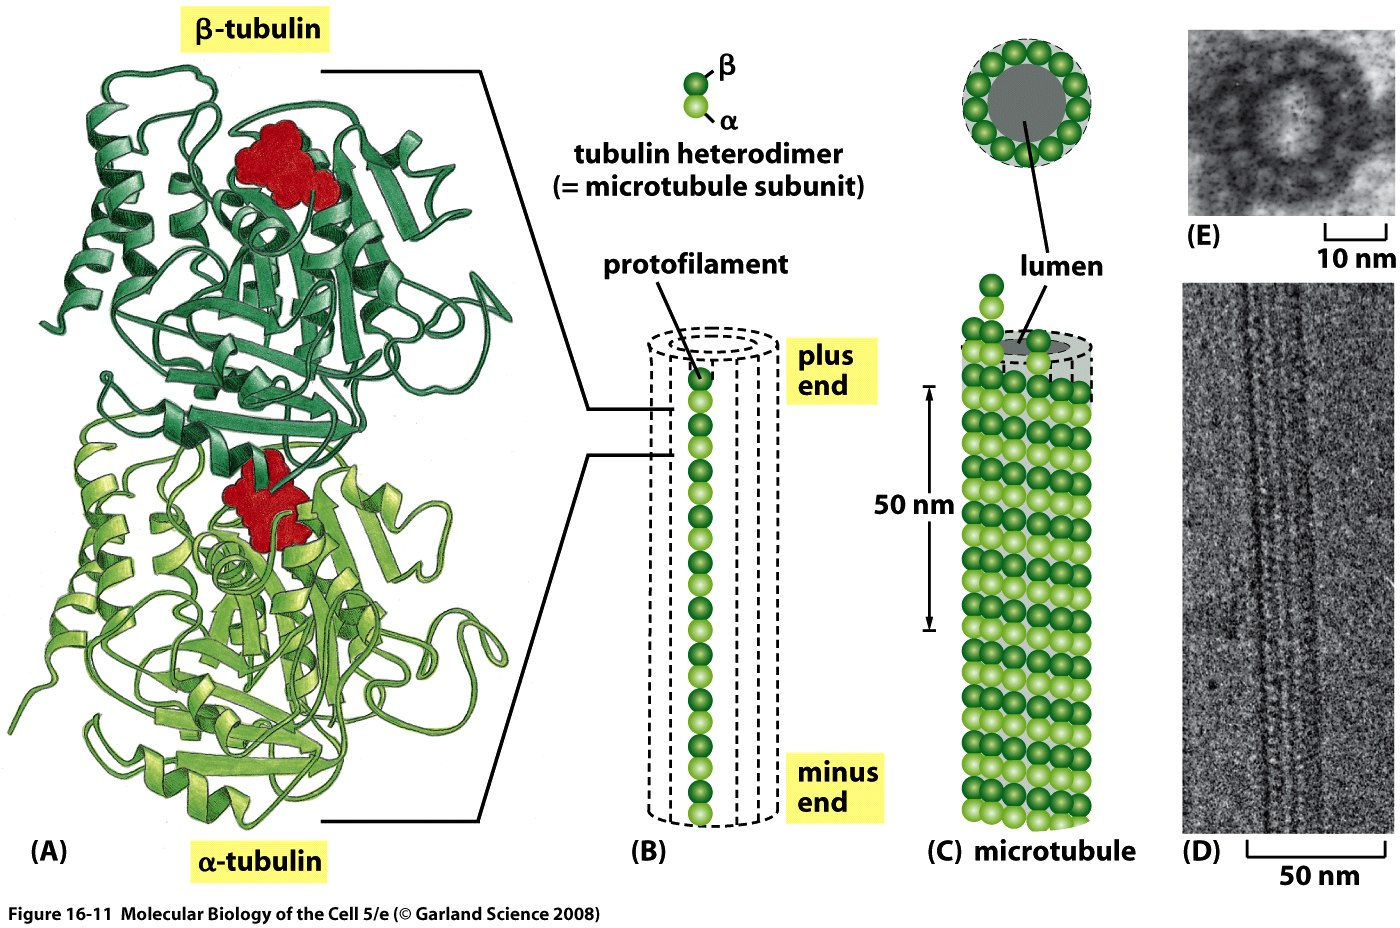
\includegraphics[width=0.700\linewidth]{microtubules-structure.jpg}
\caption{Structure of an heterodimer of tubuline and assembly into a microtubule.
Electron microscopy of a single microtubule filament. From {\hyperref[index-latex:alberts2008]{{[}Alberts, Johnson, Lewis,  et al.  2008{]}}}.
A) Structure of heterodimer of tubuline B)
Heterodimers can assemble forming polar filaments. C) Filaments can
assemble into  microtubules. D,E) Electron microscopy image of
microtubules.}\label{index-latex:fig-mt}\end{figure}

Intermediate filaments are of medium diameter in the order of around 10nm, in
between actin and microtubules filaments, hence their name.  Unlike microtubules
and actin filaments, intermediate filaments are composed by several sub-families
of proteins and are non-polar.

Intermediate filament have an important role in the mechanical properties of
cells due to the fact that they are particularly  resistant to stretching.

Unlike actin and microtubules, they are thought to be passive, with mechanical
properties mainly deriving from how multiple filaments are linked together
laterally.

Actin, is the third component of the cytoskeleton, the one on which  we will
focus on most of our efforts. Actin monomers, also called \emph{G-Actin} for globular actin can polymerise.
By polymerizing actin monomers (G-actin) into actin filaments (\emph{F-actin}), the
thinest of the three cytoskeletal components forms. Actin is produced in the
cell as a globular protein of \textasciitilde{}40 kDa (\hyperref[index-latex:fig-actin]{Fig  \ref*{index-latex:fig-actin}}) that once associated with ATP or ADP
polymerises into helicoidal filament with a diameter between 7 and 9nm. The
formed actin filaments are polar, where both extremities are respectively called the
plus (\emph{+}) or barbed end, and the minus (\emph{-}) or pointed end. The polarity of
the actin filament is of importance as this gives rise to a preferred direction
for most processes that can happen on the filaments.

The actin protein is highly conserved across species, and is know to directly
interact with hundreds of proteins {\hyperref[index-latex:dosremedios2003]{{[}DosRemedios, Chhabra, Kekic,  et al.  2003{]}}}.

Single undecorated filaments will behave  as
semi-flexible polymers at the scale of the cell with a persistence length in the order of 10 µm {\hyperref[index-latex:isambert1995]{{[}Isambert, Venier, Maggs,  et al.  1995{]}}}. When they
assemble into different structures and networks, or associate with other proteins
and molecules the resulting mechanical and dynamic properties can be highly variable.
\begin{figure}[htbp]
\centering
\capstart

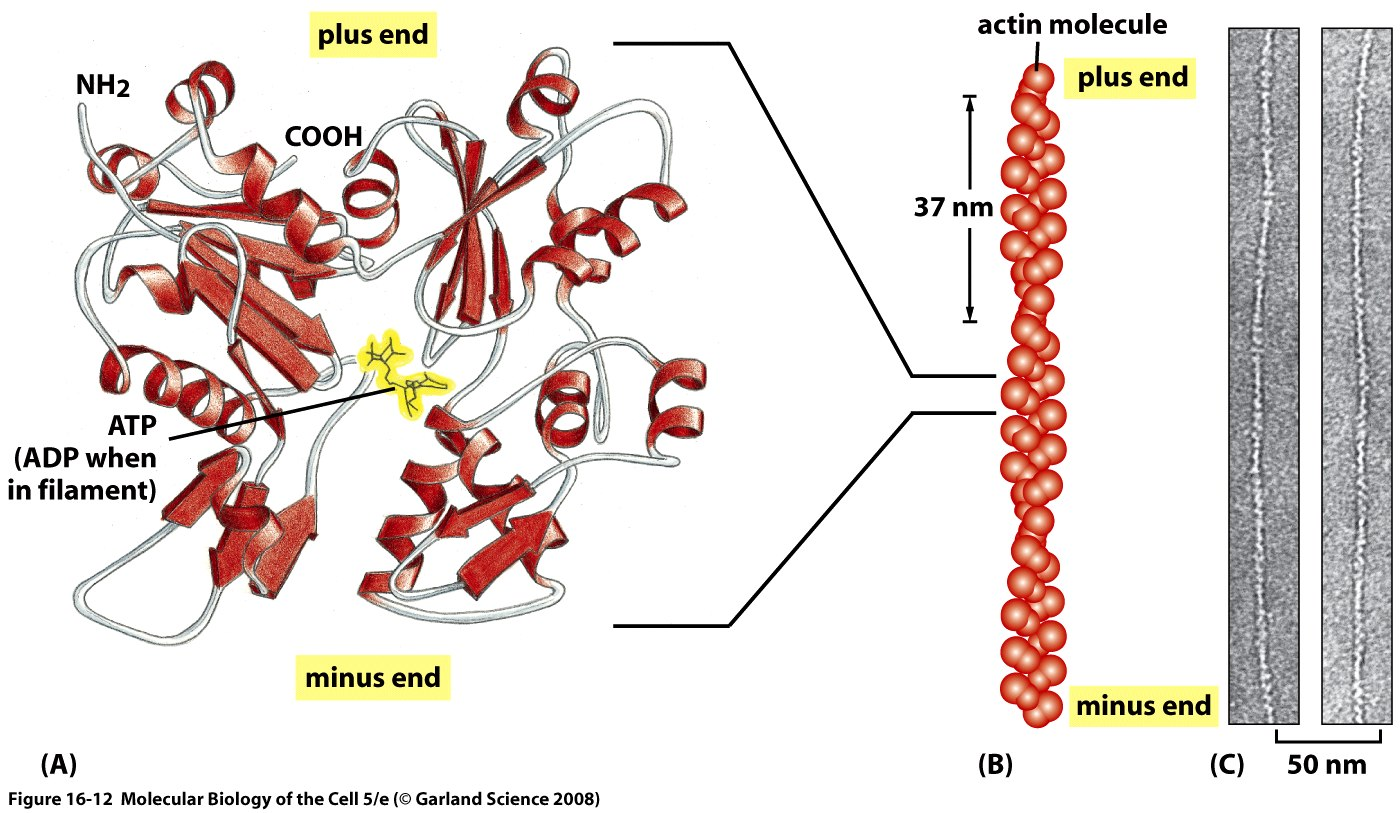
\includegraphics[width=0.700\linewidth]{actin-structure.jpg}
\caption{A) Structure of a single monomer of actin, and electron microscopy snapshot.
— from {\hyperref[index-latex:alberts2008]{{[}Alberts, Johnson, Lewis,  et al.  2008{]}}}.}\label{index-latex:fig-actin}\end{figure}


\subsubsection{Dynamics of actin polymerisation}
\label{index-latex:dynamics-of-actin-polymerisation}
The assembly mechanisms that allow to go from single monomers of actin (also
refer to as G-actin for globular actin) to actin filament (also refer as
F-actin) need to be well understood to explain the different network
structures created by actin filaments in the presence of other proteins.

The polymerisation of ATP/ADP actin monomers to form an actin filament need to
go through the step of forming an actin proto-filament which is constituted of
at least 3 actin monomers. This will most of the time be the kinetically
limiting step. Once proto-filaments are present in solution, single monomers
can be freely added or removed on both ends of the filament.  The process of
forming these proto-filaments is called nucleation and it is the rate limiting
factor to form actin filaments. To circumvent this
limitation experimentally one can use preformed actin filament seeds, or actin nucleators
to direct the polymerisation on the cell.

We need to distinguish between the dynamics of polymerisation and
depolymerisation on both ends of the filament. Indeed, it has been show that the
association and dissociation rates are differ between the pointed (-) and
barbed (+) end. The barbed end has  higher dynamics than its pointed
counterpart which is the reason for its (+) name. The dynamics of
polymerisation is higher both in he case of ATP and ADP, though the rate
constant of association and dissociation differ for both kind of filaments (\hyperref[index-latex:fig-actin-pollard]{Figure  \ref*{index-latex:fig-actin-pollard}})
\begin{figure}[htbp]
\centering
\capstart

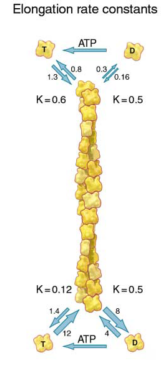
\includegraphics[width=0.250\linewidth]{elongation-rate-constant.png}
\caption{Association and dissociation rate of both ATP and ADP actin on pointed and
barbed end as measured in {\hyperref[index-latex:pollard2003]{{[}Pollard, Borisy,  2003{]}}}. The difference of
equilibrium constant between the barbed end (bottom) and pointed end (top) in the presence of ATP
allow filament treadmilling.}\label{index-latex:fig-actin-pollard}\end{figure}

The equations that drive the polymerisation can be written as follow
\phantomsection\label{index-latex:equation-roa1}\begin{gather}
\begin{split}\frac{dC_{barbed}}{dt} &= k_{+,{barbed}}.[GActin] - k_{-,{barbed}} \\
\frac{dC_{pointed}}{dt} &= k_{+,{pointed}}.[GActin] - k_{-,{pointed}} \\\end{split}\label{index-latex-roa1}
\end{gather}
Where \emph{barbed} and \emph{pointed} designate respectively the barbed and pointed end,
and \(k_+\) and \(k_-\) are the polymerisation and de-polymerisation
rate.  The concentration in barbed and pointed-end denoted by
\(C_{{barbed}/{pointed}}\). By assuming that the number of pointed ends is
equal to the number of barbed ends, one can derive the steady state which give
rise to the critical monomer concentration below which an actin filament cannot
grow: \([GActin]_c\).

The rate constants of elongation of actin have been determined and depend on
whether the monomer is bound to ADP or ATP {\hyperref[index-latex:pollard1986]{{[}Pollard,  1986{]}}}. We should
consider the fact that the  ATP bound to actin will hydrolyse to ADP-Pi before releasing
the inorganic phosphate. The hydrolysis and phosphate release rates also depend on whether the
monomer is part of a filament or in solution. The hydrolysis of ATP-bound
actin into ADP bound actin in the filament  leads to an imbalance of actin
(de)-polymerisation on both ends. The actin filaments preferably
grow from the barbed end and shrink preferably from the pointed end.

This will lead to a phenomenon known as treadmilling where a single actin
monomer bound to an ATP molecule, will be incorporated at the \emph{+} end of the
filament and progressively migrate toward the \emph{-} end, eventually hydrolysing its
ATP into ADP before detaching from the filament on the pointed end. During this
process the filament will grow / shrink until it reaches the stationary state
where its length would stay constant but the treadmilling continues.

Treadmilling requires an imbalance in the global rate constant on the barbed and
pointed end and an energy source, in the case of actin this is provided by the
hydrolysis of ATP into ADP+Pi before releasing the inorganic phosphate, without
which treadmilling would not occur.

Practically, this can be approximated by having only ATP monomers at the barbed
end of actin filaments while the pointed end is typically constituted only of
ADP monomers, thus the critical concentration is lower at the  pointed end
compared to the barbed end. The growth speed of the filament on both
ends depends on the monomer concentration in solution. In between the
critical concentration of both ends, there exists a concentration at which the
polymerisation on (+) exactly compensates the depolymerisation on (-).


\subsubsection{Actin network can be controlled by a host of actin binding proteins}
\label{index-latex:actin-network-can-be-controlled-by-a-host-of-actin-binding-proteins}
Despite the already complex process of actin polymerisation and the
number of parameters that we have already introduced, the formation of an actin
network is an even more complex process that involves many other components.
Especially, actin monomers and filaments can interact with a high number of
proteins that will affect the previously introduced dynamics.  We will present
some categories of such proteins in the following.


\paragraph{Formins}
\label{index-latex:formins}
\emph{Formins} are polymerase proteins that will increase the polymerisation rate
of actin filaments by dimerizing and binding to the barbed end. It has the
particularity of being processive, meaning that it will stay bound to the
barbed end while catalysing the addition of new monomers. The processivity of
formins also permits the control of the localization of actin polymerisation
where formin proteins are present, like the tip of filopodia {\hyperref[index-latex:faix2006]{{[}Faix, Rottner,  2006{]}}}
{\hyperref[index-latex:bornschlogl2013]{{[}Bornschlogl,  2013{]}}}. \emph{Formins} posses domains rich in proline, capable of
binding to profilin (\emph{FH1}) which allows formin to elongate F-Actin using actin
monomers bounds to profilin {\hyperref[index-latex:pruyne2002]{{[}Pruyne, Evangelista, Yang,  et al.  2002{]}}} {\hyperref[index-latex:pring2003a]{{[}Pring, Evangelista, Boone,  et al.  2003{]}}}.


\paragraph{Actin depolymerization and severing}
\label{index-latex:actin-depolymerization-and-severing}
Like polymerisation that can be enhanced by formins, depolymerization can also
be speed up. ADF/Cofilin is a protein which is able to increase the rate of
actin depolymerization. ADF/Cofilin can do so by increasing the off rate at
the pointed end {\hyperref[index-latex:carlier1997]{{[}Carlier, Laurent, Santolini,  et al.  1997{]}}}, or by actively severing the filament in
different points, thus disassembling the formed network {\hyperref[index-latex:mccullough2011]{{[}McCullough, Grintsevich, Chen,  et al.  2011{]}}}.

It should be noted that depolymerization can not only be  enhanced at the
pointed end, indeed formin that accelerate the polymerisation is also able to
speed-up the detachment of actin monomers from the barbed end.


\paragraph{Capping Protein}
\label{index-latex:capping-protein}
To regulate polymerisation, cells also have the possibility to reduce or stop
the polymerisation. To achieve this, some proteins will bind to the growing end
of actin filaments and prevent the addition of new monomers.  \emph{Capping Protein}
(CP) being one particular example that will specifically bind to the barbed end
of a growing filament and  prevent it from growing. Capping proteins are
necessary to prevent polymerisation of actin in undesired area
and are essential for the structure and mechanical properties of actin gel
{\hyperref[index-latex:kawska2012]{{[}Kawska, Carvalho, Manzi,  et al.  2012{]}}}. \emph{Gelsoline} is another example of Capping Protein, that
unlike CP can only attached to the barbed end of an actin filament after
severing it. Gelsoline is hence both a severing and a Capping Protein.


\paragraph{Cross-linkers}
\label{index-latex:cross-linkers}
We have seen that some proteins were able to attach to actin filaments. When
such a protein is able to attach to many filament at once, it can act as an
attachment point between the two filament, preventing them to move with respect
one to each other. Such proteins, are referred to as cross-linkers.

The amount of freedom in movement between the two filaments depends on the
cross-linker used. For example , \(\alpha\)-actinin will allow rotation of the two
filament at their anchoring point whereas cross-linkers like fascine will prefer
a parallel conformation of the filament and favor the formation of actin
bundles.

Cross-linkers are essential for the formation of elastic network as they allow
forces to be carried from one actin filament to the other. The quantity of
cross link of a network will often be a key parameter for the elastic properties.
The distance between the link points in the network (both cross links
and entanglement points) will give the typical network mesh-size which is used
to calculate the viscoelastic response of networks : {\hyperref[index-latex:morse1998a]{{[}Morse,  1998a{]}}}.


\paragraph{Stabilizing actin filaments}
\label{index-latex:stabilizing-actin-filaments}
As actin networks are dynamic constructs that are changing shape and properties
over time, it is convenient to be able to stabilize those networks. Tropomyosins
are proteins capable to bind on the side of actin filament to stabilize them.

The use of phalloidin, a toxin extracted from fungus (Amanita phalloides), binds
between F-actin subunits on the filament, and hence  prevents it from
de-polymerising.  Though, it is known that stabilizing actin filaments with
phalloidin will increase their stiffness as measure by the persistence length which can change the
mechanical properties of the formed actin network.


\paragraph{Profilin}
\label{index-latex:profilin}
Profilin is a protein that will bind to the barbed end of single monomers of
actin in solution.  By doing so it will first prevent the association of
monomers into dimers and trimmers, thus preventing the nucleation of actin
filament. It thus allows a better control of localisation of actin filament
both in vivo and in vitro in the presence of actin seeds of actin nucleator.

Profilin was for a long time believed to be only a sequestering protein
that inhibit polymerisation {\hyperref[index-latex:yarmola2009]{{[}Yarmola, Bubb,  2009{]}}}, though it has a more complex
behavior, and if it prevent polymerisation of actin filaments by the pointed
end, it can facilitate polymerisation. One of the cause of increase in
polymerisation speed by profilin is the fact it binds preferably to ADP-Actin
and increase the exchange rate of ADP into ATP.


\paragraph{Branching Agent}
\label{index-latex:branching-agent}
A type of network found of the leading edge of cells lamellipodia is dendritic
network. It is characterised by tree-like structure of actin filaments in which
thanks to the Arp2/3 complex branching agent a mother actin filament will form a
daughter filament on its side.

We have seen previously that crosslinkers are proteins capable of linking two
or more actin filaments together by binding on their side. Another mechanism
involving binding on the side on actin filament is responsible for a closely
related network, the branching mechanism.

The Arp2/3 complex is composed of seven subunits, two of which are highly
similar to actin, forming the Arp2 and Arp3 family for Actin Related Proteins,
giving the complex its name. Typically Arp2/3 will bind on the side of a pre-existing
actin filament, hence initiating the growth of a daughter filament with an angle of
70° to the mother filament. The newly created daughter filament pointed end
is terminated by the Arp2/3 complex that will stay attached to the mother
filament, thus increasing the number of available barbed end, without changing
the number of available pointed end. See Nature Review by Erin D. Goley and
Matthew D. Welch {\hyperref[index-latex:goley2006]{{[}Goley, Welch,  2006{]}}} for  a longer review about the Arp2/3
complex.

In cells, the Arp2/3 complex needs to be activated by a Nucleation Promoting
Factor (NFP).  Among them is the  WASp protein (Wiskott-Aldrich Syndrome
protein) and its neural homologue N-WASP which are from the same family as
SCAR/WAVE {\hyperref[index-latex:machesky1999]{{[}Machesky, Mullins, Higgs,  et al.  1999{]}}}.  All these activators of Arp2/3 have in common a
WCA motif. The wild type protein need to be activated in order to activate Arp2/3.
The activation is done by a change in conformation that exposes the active
region and provides the first actin monomer necessary for nucleation of the
daughter filament (\hyperref[index-latex:fig-pwa-deploy]{Figure  \ref*{index-latex:fig-pwa-deploy}}).  To circumvent the activation process of
these proteins, we use a reconstructed version of the protein that cut all
region before the poly-proline. This confer to pVCA the ability to be
permanently active. This region can also be replaced by streptavidin in order
to selectively bind pVCA to selected regions. Characterisation and more
detailed description of pVCA can be found in {\hyperref[index-latex:noguera2012]{{[}Noguera,  2012{]}}}.
\begin{figure}[htbp]
\centering
\capstart

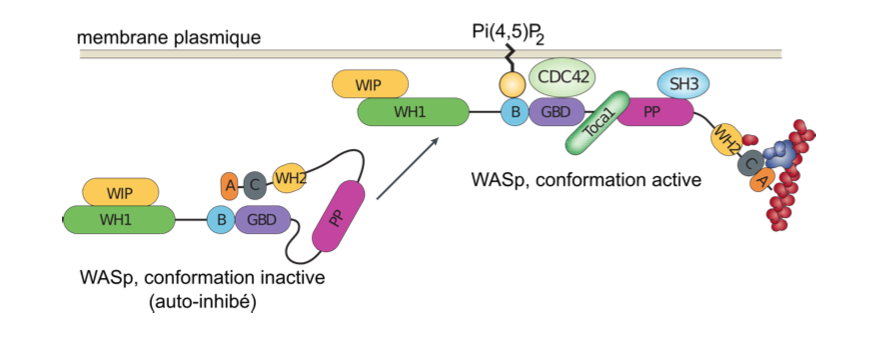
\includegraphics[width=0.600\linewidth]{pwa-deploy.png}
\caption{Organisation of Wasp domains. A change in conformation make the protein
active, which allow the activation of the Arp2/3 complex and the nucleation
of a daughter filament.  Adapted from {\hyperref[index-latex:goley2006]{{[}Goley, Welch,  2006{]}}}}\label{index-latex:fig-pwa-deploy}\end{figure}

Unlike Cells that are able to control the localisation of actin nucleation
processes thanks to activation of WASp and its homologue, the `in vitro' control
of localisation of actin polymerisation is directly done by the localisation of
pVCA.

The network formed by Arp2/3 is called a dendritic network, and is in
particular found at the leading edge of the cell in the lamellipodia. It is
such a network that is present in the bead system we will study hereafter.

As for crosslinkers, dendritic networks are able to carry forces across single
actin filaments by the intermediary of Arp2/3. Two dendritic network of Arp2/3
can also entangle and allow forces to be carried across them
{\hyperref[index-latex:kawska2012]{{[}Kawska, Carvalho, Manzi,  et al.  2012{]}}}.
\begin{figure}[htbp]
\centering
\capstart

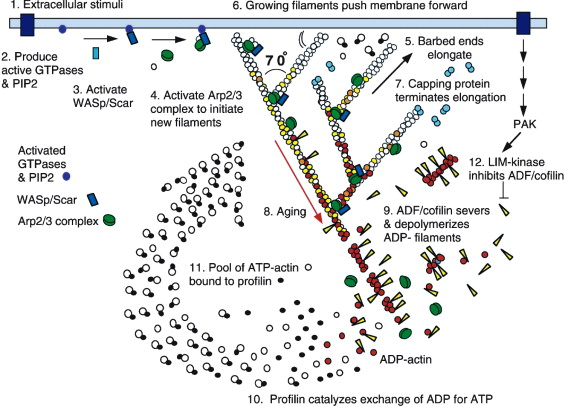
\includegraphics[width=0.700\linewidth]{pollard2003-actin-cycle.jpg}
\caption{Schematic recapitulating the formation of
a dendritic network at the leading edge of a cell were several of the
function of protein can be seen. An actin nucleation promoting factor
(Active WASp,  blue rectangle at the membrane) will activate Arp2/3 (green
blob) which will act both as nucleation factor and a branching agent. From
an activated Arp2/3 will grow an actin filament pointing towards the
membrane. Newly growing barbed ends, rich in ATP-actin (white circle) can
eventually be capped by Capping Protein (light-blue pairs of circle) which
will terminate their growth.  Aging monomers in actin filament will slowly
hydrolyse their ATP (yellow and red circle), eventually releasing the
inorganic phosphate before detaching from the pointed end.
Depolymerisation is helped by severing protein (sharp triangle) and Actin
Depolymerisation Factor (ADF). ADP-actin monomer will bind to profilin
(Black dots) increasing the turn over rate to ATP-actin which will be reused
by the leading edge of the cell. Adapted from {\hyperref[index-latex:pollard2000]{{[}Pollard, Blanchoin, Mullins,  2000{]}}}.}\label{index-latex:actin-cycle}\end{figure}

A schematic that recapitulate the interaction of actin with other protein and
the formation of a dendritic network at the leading edge of the cell is
presented on \hyperref[index-latex:actin-cycle]{figure  \ref*{index-latex:actin-cycle}}.


\paragraph{Molecular Motor}
\label{index-latex:molecular-motor}
A particular kind of protein that can bind to the cytoskeletal filaments are
molecular motors. Molecular motors are proteins that will consume energy
in the form of ATP, hydrolyse it to change conformation and produce forces.

The motors that move along actin filaments are part of the myosin superfamily, they
are both responsible for the transport of cargo along filaments, cell motility,
division, and muscle contraction. They acquire their name from their discovery
in 1864 by Willy Kühne who extracted the first myosin II extract from muscle
cell {\hyperref[index-latex:hartman2012]{{[}Hartman, Spudich,  2012{]}}}.

The myosin super family is divided into subfamilies numbered with roman literals.
As of today we count more than 30 families of myosin {\hyperref[index-latex:berridge2012a]{{[}Berridge,  2012{]}}}.
Muscle myosin is part of the myosin II family and is often referred to  as
conventional myosin for historical reason as being the first discovered.
Non-muscle  myosin are also referred to as unconventional myosin.

Myosin motors seem to be shared among the living domain, hinting for an
early emerging of myosin in the evolution. All the myosin motors move on actin
filaments toward the barbed end, with the exception of myosin VI which moves
towards the pointed end {\hyperref[index-latex:buss2008]{{[}Buss, KendrickJones,  2008{]}}}.

Different subfamily of myosin are used for different function in cells. Even in
subfamilies each type of myosin can have specific functions. For example,
conventional myosin found in muscle cells are use for large scale cell
contraction. In contrast, myosin V is known to transport cargo and is found to
be responsible for actin network dynamics and vesicle positioning
{\hyperref[index-latex:holubcova2013]{{[}Holubcova, Howard, Schuh,  2013{]}}}.


\subparagraph{Myosin II}
\label{index-latex:myosin-ii}\label{index-latex:myoii}
As stated before, the myosin II family both encompass conventional myosin as
well as Non-muscle myosin II (NMII). Both have a similar structure (\hyperref[index-latex:fig-myosin]{Fig  \ref*{index-latex:fig-myosin}}).

All myosin IIs are dimers constituted of two heavy chains and light chains. The
heavy chains are held together by a coil-coiled alpha helix referred to as the
tail. On the other side of the protein sequence is a globular head, which is
responsible for ATP hydrolysis and is able to convert the energy from the
hydrolysis into mechanical force. It is also the part that will bind to the
actin filaments. In between the tail and head is the neck domain that acts as a
lever to transmit the force generated by the head to the tail. The length of
the neck influences the length of the movement done by the cargo at each step of
the myosin as well as the size of the step the myosin can effect. The two light
chains are situated in the neck region and are responsible for the myosin
activity regulation.

Myosin II dimers can align and assemble by the tail region, forming myosin
minifilaments. These minifilaments are bipolar, having numbers of myosin head
with the same orientation at each extremity.

In the myosin II family, conventional myosin and NMII differentiate by the
size of the minifilaments they form. Muscle myosin will form minifilaments
aggregating around 200 dimers, where NMII minifilaments will be composed  only
of 10 to 20 minifilaments. The other characteristic of unconventional myosin
with muscle myosin is the mode of activation. Conventional myosin activity is
regulated by the amount of \(Ca^{2+}\) available, which frees the actin filaments to let the myosin motor bind. However, its
counterparts are typically activated by the phosphorilation of the Myosin Light Chain (MLC).

Another parameter that discriminates muscle from non-cell myosin is their duty
ratio.  The duty ratio is define as the ratio of the time the myosin stays
attached to an actin filament over the typical time of a contraction cycle.
By noting \(\tau_{on}\) and \(\tau_{off}\) the time the myosin head
spent attached/detached from  the filament, the duty-ratio or duty-cycle can
be noted :
\phantomsection\label{index-latex:equation-roa2}\begin{gather}
\begin{split}r = \frac{\tau_{on}}{\tau_{on}+\tau_{off}}\end{split}\label{index-latex-roa2}
\end{gather}
We will see in the following that the duty-ratio might have an important effect
on the processivity of the myosin.

It should be noted that as minifilaments can attach to actin filaments on both
ends, they can also act as a bridge that holds two points close to each other,
though having the properties of crosslinkers.


\subparagraph{Myosin V}
\label{index-latex:myosin-v}
Myosin V is an unconventional myosin. Unlike myosin II it does not aggregate
into minifilaments.  Though, myosin V has a similar structure to myosin II but
with a longer neck, this confers to myosin V the ability to realize longer
steps on actin filaments. Indeed, the myosin V step size is of 36nm, which is close to the
twisting length of actin filaments. This allows myosin V motors to walk along
actin filament without having to rotate around it with the helix they form. At the end the tail domain
myosin V posses another globular domain capable of binding to its cargo, and
the variability of this region is what mostly define the difference between the
different type of myosin V.

Myosin V also has a high duty-ratio, this leads to dimers having almost always
one of the two head of the myosin to be bound to actin. It grants to the myosin
V the ability to walk in a processive manner toward the barbed end of
the actin filaments, both head successively binding 36 nm in front of the other
head.
\begin{figure}[htbp]
\centering
\capstart

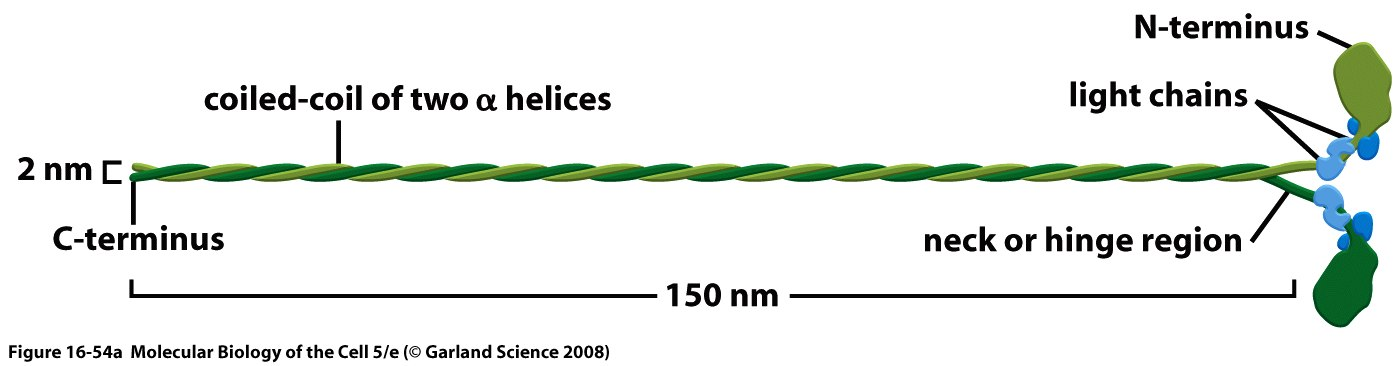
\includegraphics[width=0.700\linewidth]{figure-16-54a.jpg}
\caption{Schematic of a dimer of myosin motors with the example of Myosin II.
Each of the myosin monomer is colored in a
different shade of green. From Right to Left, the myosin head, with the N
terminal, is the part of the myosin that binds to the actin filaments. The
neck region with the light chain act as a lever arm. Finally the tail,
constituted with coiled-coil alpha-helix that aggregate to form minifilaments.
Adapted from {\hyperref[index-latex:alberts2008]{{[}Alberts, Johnson, Lewis,  et al.  2008{]}}}.}\label{index-latex:fig-myosin}\end{figure}


\subparagraph{Myosin cycle}
\label{index-latex:myosin-cycle}
We saw earlier that the duty ratio of myosin was the ratio of time the head of
the myosin spent attached to the actin filament. Indeed, myosin can generate
displacement through a cycle of ATP hydrolysis and attachment/detachment
described below for a Myosin II motor:

The cycle can be decomposed in 5 steps, last of which will be responsible for
the forced exerted on the myosin cargo.
\begin{itemize}
\item {} 
The myosin start in the `rigor' conformation where it is lightly bound to
the actin filament.

\item {} 
An ATP molecule binds to the myosin head inducing the detachment of the
myosin from the actin filament.

\item {} 
ATP molecule is hydrolysed into ADP+Pi, providing energy which is stored
into a conformational change of the myosin which effects a recovery
stroke.

\item {} 
Inorganic phosphate is released as the myosin head attaches to the actin
filament.

\item {} 
The actin-bound myosin change conformation, applying forces on it's
cargo. This step is known as the power-stroke and is responsible for most
of the applied forces or displacements of the myosin. During the
power-stroke the ADP bound to the myosin head is released, leading back
to first step of the cycle.

\end{itemize}

This principle is the same for all kinds of myosins. In the case of Myosin II
the duty-ratio is only of about 5\%, which leave Myosin II detached from the
actin filament most of the time. A single dimer cannot achieve
processivity.   The tail of myosin II can bundle itself with the tail of other
myosin II motors.  They from large bipolar thick filaments of hundreds of dimers.
As each myosin dimer attaches and detaches independently from the actin
network the effective attachment of of the filament increases with the number
of motors in the minifilaments. Indeed the probability of having at least one
motor attached increases with the number of motors. The constant attachment of
at least one myosin II head in minifilaments insure that the filament does not
displace with respect to the actin network when others myosin heads recover
from their power stroke and reattach, thus conferring processivity to myosin II
minifilaments.

The bipolar nature of myosin II minifilaments also allow them to act as force
dipoles, each  of the extremity pulling the surrounding actin network or
filament towards the center of the minifilaments. This is the mechanism at the
origin of muscle contraction and can allow to build-up tension in actin network.


\subsection{The actin cortex}
\label{index-latex:the-actin-cortex}
The actin cortex is a thin layer of between 200 to 500 nm that can be found
just underneath the plasma membrane of a cell (\hyperref[index-latex:fig-electro-cortex]{Fig  \ref*{index-latex:fig-electro-cortex}}) . The properties of the actin
cortex makes it a key component to diverse processes.  Its capacity to resit
to, and transmit forces is indispensable for locomotion of many cells by
allowing the retraction of the rear of the migrating cell and will be describe
in more detail in the next section. Its structure is also essential for the
cellular division as contractility is necessary to generate cortical tension
and achieve the separation of the two daughter cells.

The actin cortex is constituted of actin filaments that can be parallel or
orthogonal to the membrane as one can see using electron microscopy on cells
{\hyperref[index-latex:morone2006b]{{[}Morone, Fujiwara, Murase,  et al.  2006{]}}}.
\begin{figure}[htbp]
\centering
\capstart

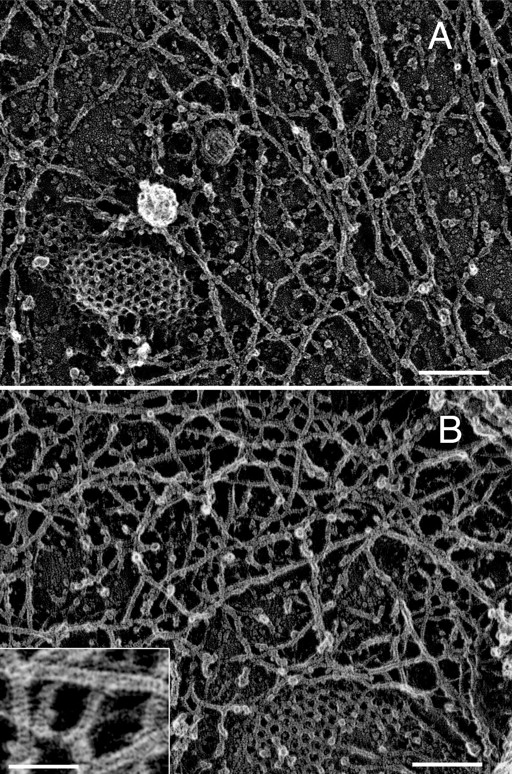
\includegraphics[width=0.700\linewidth]{Actin-Cortex-Moronne-2006.jpg}
\caption{Electron microscope view of the actin cortex in rat cell. The inset
show a periodicity of \textasciitilde{}5nm in filaments characteristic for actin.  Scale
bars are 100nm, inset 50 nm. Extracted from {\hyperref[index-latex:morone2006b]{{[}Morone, Fujiwara, Murase,  et al.  2006{]}}}.}\label{index-latex:fig-electro-cortex}\end{figure}

We saw through the bud scar of budding yeast that the full cytoskeleton could
retain memory of past events. It is also the case for simple actin networks as
show in {\hyperref[index-latex:parekh2005]{{[}Parekh, Chaudhuri, Theriot, Fletcher,  2005{]}}} who describe how actin-network growth can be
determined by network history, showing actin cortex could also act as a memory
for cell.


\subsection{Cell Motility}
\label{index-latex:cell-motility}
The way cells move highly depends on their environment and the cell type.
We can distinguish several strategies of movement, mainly categorised into
amoeboid and mesenchymal movement. The type of motility for certain
cells can be characteristic for malignant tissue, and plays a significant role in
the ability of the cells to invade nearby tissues.
\begin{figure}[htbp]
\centering
\capstart

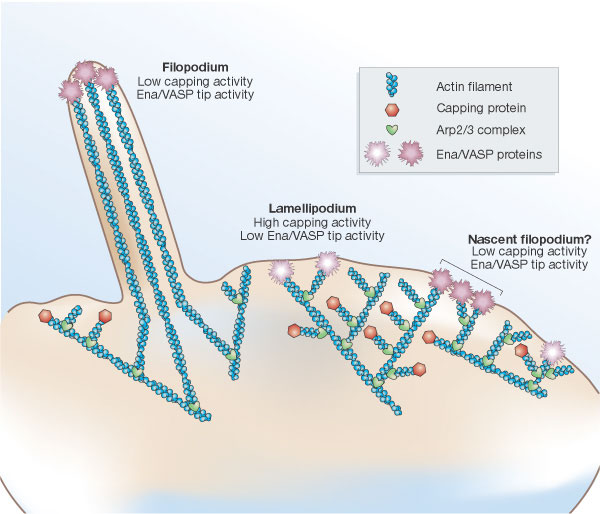
\includegraphics[width=0.600\linewidth]{Schafer2004.jpg}
\caption{Polymerisation at the leading edge of the cell. NPF situated on the
membrane of the cell localize the polymerisation. The lamellipodium will be
characterized by a dendritic network formed by Arp2/3. Parallel actin
structures can form a growing protrusion called filopodium.  Adapted form
{\hyperref[index-latex:schafer2004]{{[}Schafer,  2004{]}}}}\label{index-latex:fig-schafer}\end{figure}


\subsubsection{Lamellipodium based Motility}
\label{index-latex:lamellipodium-based-motility}
We can ave a first look into the mesenchymal mode of locomotion of cells, which is
also often referred to as crawling. To understand how a cell is able to crawl,
to move itself, we will in particular take the example of the lamellipodium.
The lamellipodium is a characteristic structure found in cells moving on a 2D substrate. By
its nature, motion using lamellipodia is one of the easiest to study using
microscopy which might explain why it is one of the best know process of cell
displacement. None the less, it does not diminish its importance in tissues
behavior as all epithelial cell can be considered as moving on a 2D substrate.
Beyond lamellipodia, further structures that are responsible for cell motion are
filopodia and pseudopodia. They mainly differ from lamellipodia by their shape
and the organisation of the actin structure inside (\hyperref[index-latex:fig-schafer]{Fig  \ref*{index-latex:fig-schafer}}). Lamellipodia-based motion
can move a cell up to a few micrometers per minute.

The action necessary to move in an mesenchymal way can be decomposed into three
steps. First the cell needs to grow a protrusion. Growing this protrusion is
typically governed by actin polymerisation just underneath the plasma membrane. The
lamellipodium is such a protrusion which is constituted by a 2D dendritic actin network
that polymerize at the leading edge. Second the cell's protrusion
need to attach to the surface. This is done through trans membrane proteins
that are bound to the actin cortex on the inside of the cell. The actin cortex
will act as a scaffold to transmit the force across the cellular to these
anchor points. The last part is the generation of traction in which the rest of the cell is pulled
toward the attached protrusion. The traction force is mediated through the
cytoskeleton and actin cortex while the contraction force themselves can origin
from actin network contraction and reorganisation due to myosin motors (\hyperref[index-latex:fig-lam-principle]{Fig  \ref*{index-latex:fig-lam-principle}}).
\begin{figure}[htbp]
\centering
\capstart

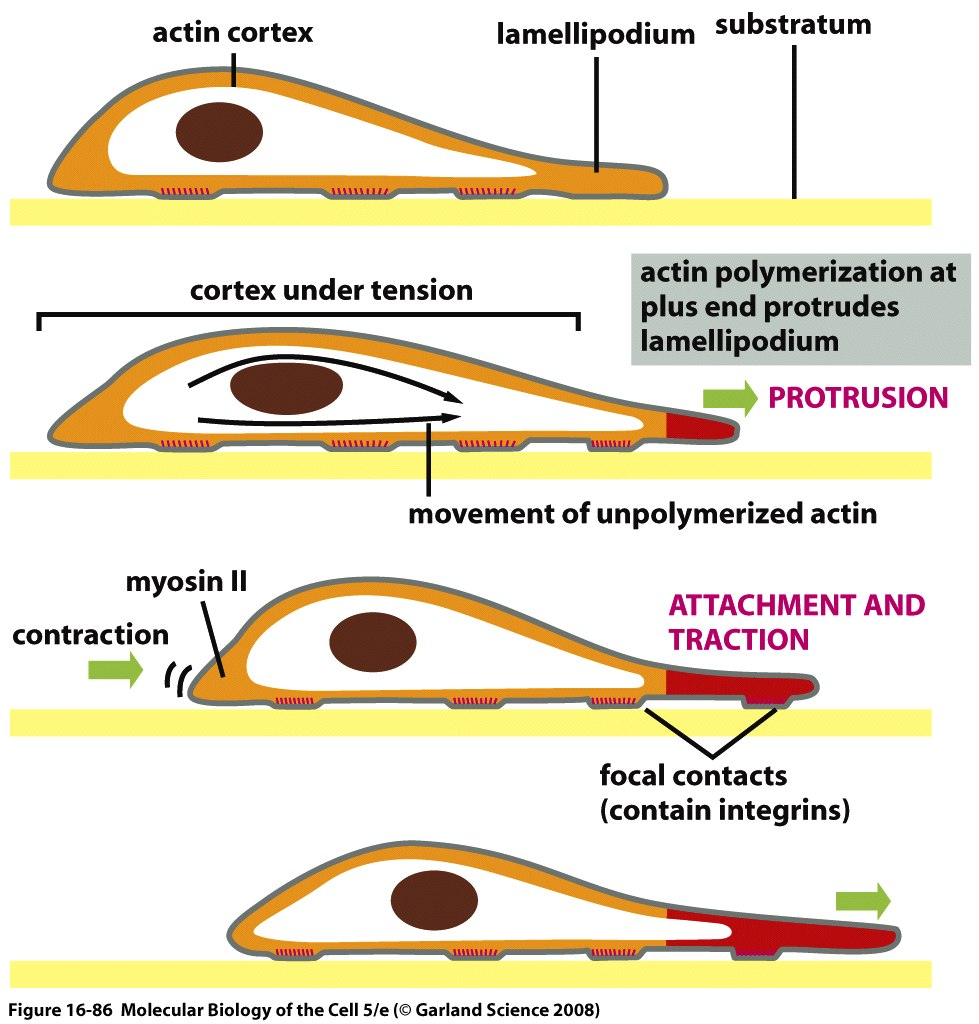
\includegraphics[width=0.900\linewidth]{figure-16-86.jpg}
\caption{Schematic of Lamellipodium base motility. The lamellipodium grows at the
leading edge of the cell and attach to a focal point. The actin cortex
under tension contract and is capable to pull the rear of the cell. Adapted
from {\hyperref[index-latex:alberts2008]{{[}Alberts, Johnson, Lewis,  et al.  2008{]}}}.}\label{index-latex:fig-lam-principle}\end{figure}


\subsubsection{Blebbing based Motility}
\label{index-latex:blebbing-based-motility}
The second mode of motility which is known as amoeboid is more characteristic
of 3D displacement of cells. In this mode, the cell will also form protrusions
but will not rely on adhesion to move its body. This motility rely on blebs,
that are blister-like protrusion that appear on the cell surface. A bleb
forms on the surface of cell when the membrane detach from the actin
cytoskeleton underneath it, or when the cortex ruptures (\hyperref[index-latex:fig-bleb]{Fig  \ref*{index-latex:fig-bleb}}). The small protrusions
are formed, quickly grow as they lack the force supporting layer that the actin
cortex provides. While growing, the bleb fills with cytosol. The actin
cortex can rapidly reform on the bleb slowing down its growth. In some cases,
the reformation of the actin cortex in the bleb and the rebuilding of the
tension inside the bleb by myosins mediated contraction is enough to reverse
the bleb. Though, the content of the cell can also drain itself into the bleb
as it grows and while the main body of the cell contract and empties, thus
moving the cell from its old position to a new one in the direction of the
initial growth of the bleb.

At their initial state, blebs are simple membrane protrusions filled with
cytosol and empty of organelles. The stop of their growth is due to the
spontaneous formation of an actin cortex on the inner side of the bare
membrane.

By their relative simplicity to the rest of the cells, blebs are the perfect
system to be reconstituted \emph{in vitro} in liposomes.
\begin{figure}[htbp]
\centering
\capstart

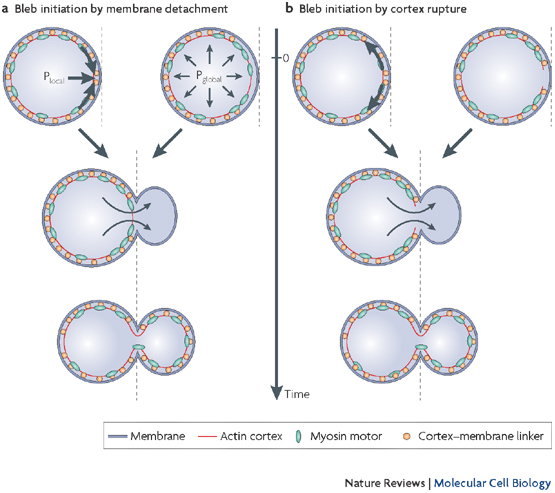
\includegraphics[width=0.400\linewidth]{Bleb-nature-paluch.jpg}
\caption{Formation of bleb can be done either by a) detachment of the membrane from
the cytoskeleton, or b) by a rupture of the cytoskeleton. In both cases the
inner pressure of the cell leads to the inflation of the membrane at the
point of rupture/detachment. The acto-myosin cortex will rapidly re-polymerize on
the inside of the bleb slowing down its growth until the expansion stops.
Extracted from {\hyperref[index-latex:charras2008]{{[}Charras, Paluch,  2008{]}}}}\label{index-latex:fig-bleb}\end{figure}


\subsection{Organelle Positioning}
\label{index-latex:organelle-positioning}\label{index-latex:id42}
We have seen previously that organelle positioning plays an important role in
cell function.  Several mechanisms involving actin are at the origin of
structure positioning in cells. The positioning of organelles by actin can have
a wide impact from being necessary for the correct cell division, to
allowing locust eyes to adapt in the dark by repositioning mitocondrion
{\hyperref[index-latex:sturmer1995]{{[}Sturmer, Baumann, Walz,  1995{]}}}.

We already know that the actin cortex is a necessary element in cell
motility. It also plays a determinant  role in organelle
positioning. It has been shown  {\hyperref[index-latex:chaigne2013a]{{[}Chaigne, Campillo, Gov,  et al.  2013{]}}} that the correct range
of elasticity of the actin cortex during oocyte division is needed for proper spindle
positioning. The correct spatial position of this spindle is necessary to
perform a viable division of the cell.

The actin cortex is not the only actin structure in the cell, beyond the thin and
dense layer just below the membrane lies a softer and sparser actin structure that has a
crucial role in organelle positioning.

During cell division, there are several stages that require actin structures.
As shown previously {\hyperref[index-latex:azoury2011]{{[}Azoury, Lee, Georget,  et al.  2011{]}}} the expulsion of polar body during
oocyte asymmetric division is  strongly dependent on the time evolution of a
sparse actin network that can be found in the cell. Actin structures are  also
required at a later stage to permit the correct capture of chromosomes by
microtubules and achieve correct haploid division.  {\hyperref[index-latex:schuh2008]{{[}Schuh, Ellenberg,  2008{]}}} also shows
that a similar sparse actin network contracted by myosins is necessary for
spindle migration.

Especially in oocyte that are typically large, the effect of gravity is not
negligible. The presence of a sparse ``actin scaffold'' is discussed in
{\hyperref[index-latex:feric2013]{{[}Feric, Brangwynne,  2013{]}}}, where it is found that an actin network is present to
balance the gravitational force.

In drosophila, nurses cell need to expel their content into oocytes. It has been
observed {\hyperref[index-latex:huelsmann2013]{{[}Huelsmann, Ylanne, Brown,  2013{]}}} that during this phase, the nurse cells' nucleus
is pushed away from the dumping canal by single actin filaments polymerising
from the membrane and forming a soft and sparse actin network.


\section{In vitro reconstituted actin networks}
\label{index-latex:in-vitro-reconstituted-actin-networks}
Living cells are complex organisms, for which each function requires a number
of interacting proteins and components. To understand the action of each
individual component it is necessary to isolate or modify their actions
independently.

In order to achieve the precise tuning of each component independently, two
approaches are envisageable. An approach referred to  as ``Top-Down'' where
starting from the full system — in our case the cell — we will modify or remove
single or multiple components and study the global change of behavior. This is a complex
process that might be difficult to interpret as biological systems have often
multiple pathways and feedback loops to regulate each of their processes. With the
large number of components that constitute a living cell, it is also
difficult to come up with a minimal system necessary to replicate certain behavior.

The other approach, also referred to as the bottom-up approach, requires to
reconstitute the system part by part until it replicates the expected
behavior. This is also a complex process, as there is a large number of potential component
that may be added to the reconstituted system. Often this vast complexity
leads to a wide range of testable parameters.
These controlled systems allow in principle for a deeper understanding of the governing
working mechanisms, and often permit access to a wider range of accessible
conditions and individual tweaking of components.

In our lab we are mainly interested in the bottom-up approach and the use of
biomimetic systems. We try to reconstitute biologically relevant behavior within
minimal systems,  constituted from pure protein components.

In particular in this manuscript we are interested in mimicking the motility process
by which the \emph{listeria} pathogen is able to hijack cellular mechanisms by recruiting proteins
responsible for actin polymerisation at the leading edge of the cell, and use
these to polymerize actin on the pathogen surface. This is what allows `listeria' to
propel itself fast enough (1.5 to 2 µm /min) {\hyperref[index-latex:dabiri1990]{{[}Dabiri, Sanger, Portnoy, Southwick,  1990{]}}} to be able to
penetrate the cell membrane to move from one cell to the other.

The bead motility system is a minimal \emph{in-vitro} system capable of replicating
the listeria motility.


\subsection{Bead motility assay}
\label{index-latex:bead-motility-assay}\label{index-latex:id50}
The \emph{Listeria} pathogen is a 1.5 to 5 micrometer cylindrical bacteria that
enter cells, hijacks its actin polymerisation machinery to propel itself and
infect neighbour cells. It does so by the recruitment of a single protein on its
surface : ActA, that activates the Arp2/3 complex. By the recruitment of Arp2/3 a
dense branched and entangle actin network grows that will eventually form a
comet behind the bacteria propelling it at the speed of actin comet
polymerisation. Listeria comets are composed of a wide range of protein, it has
been shown {\hyperref[index-latex:loisel1999]{{[}Loisel, Boujemaa, Pantaloni, Carlier,  1999{]}}} that the number of required components can
be highly reduced, still maintaining the motility features.

A simpler system replicating the listeria motility is the bead
motility assay, which consists of a micrometer-sized bead covered with a nucleation
promoting factor (NPF) that will activate Arp2/3 that is present in solution.  This NPF can
be ActA as in the case of listeria, but one can use other NPF like N-WASp or
pVCA. In the experiments presented in this work we use pVCA. The NPF covered
bead is mixed with a G-Actin solution. Capping Protein is added to prevent
polymerisation from happening away from the bead surface as well as the
components necessary for actin polymerisation (ATP, Salt..., see {\hyperref[index-latex:m-et-m]{\emph{Material and methods}}} (\autopageref*{index-latex:m-et-m}))

Due to the presence of Capping Protein in solution and NPF on the surface of
the bead, the polymerisation of actin will happen only on the surface on the
bead forming a thin and dense actin gel capable of sustaining stress depending
on the different protein concentrations. Unlike in the case of listeria which
seem to control on which of its sides the nucleation process happens, this is not
controlled in bead motility assays. Though, in the right condition
{\hyperref[index-latex:kawska2012]{{[}Kawska, Carvalho, Manzi,  et al.  2012{]}}} the dense actin gel formed on the bead surface can
accumulate stress induce by polymerisation of inner layer until symmetry
breaking occurs. The gels ruptures on one of the side of the bead, leading to
the formation of a comet on the opposite side (\hyperref[index-latex:fig-bead-motility]{Fig  \ref*{index-latex:fig-bead-motility}}).
\begin{figure}[htbp]
\centering
\capstart

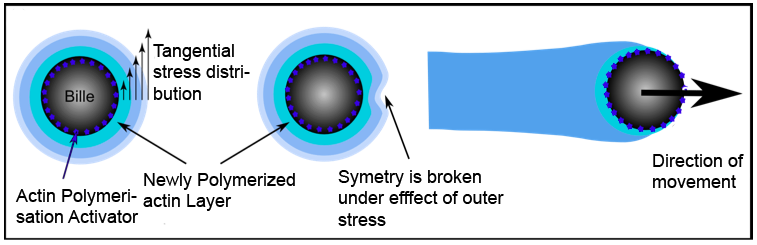
\includegraphics[width=0.600\linewidth]{Plastino-Sykes-2005.png}
\caption{Scheme of bead motility assay. The NPF (yellow stars) will localize the
actin polymerisation on the surface of the bead thus increasing stress on
the outer actin layer. At a sufficient level of stress, the outer layer
ruptures, leading to symmetry breaking, formation of a comet, and
propulsion of the bead. Adapted from {\hyperref[index-latex:plastino2005]{{[}Plastino, Sykes,  2005{]}}}}\label{index-latex:fig-bead-motility}\end{figure}

The further polymerisation of the actin network on the surface of the bead will
make the comet grow, propelling the bead forward. This is what makes the bead
system a biomimetic system replicating the listeria motion.

It should be noted that during the movement of this system, two phases can be
distinguished. In the first phase, the system present a spherical symmetry with
an homogeneous actin  network around the bead. The gel is growing from the
surface and is accumulating stress due to the polymerisation of inner layers.

If the gel had accumulated sufficient stress by polymerisation  the symmetry breaking event happens, and the system enters in
a second phase with the formation of a comet.

The condition that lead to symmetry breaking have been investigated in detail
{\hyperref[index-latex:kawska2012]{{[}Kawska, Carvalho, Manzi,  et al.  2012{]}}}. In the absence of Capping Protein, the actin polymerisation seems
not to be restricted enough near the surface of the bead, and the formed
network is not able to generate or sustain enough stress to achieve symmetry
breaking. At high Capping Protein concentration, the growth of the gel is heavily impaired,
thus preventing symmetry breaking. The concentration of Arp2/3 is also critical
as Arp2/3 forms branched networks, and these branched networks are primordial for the
ability to sustain stress.
\begin{figure}[htbp]
\centering
\capstart

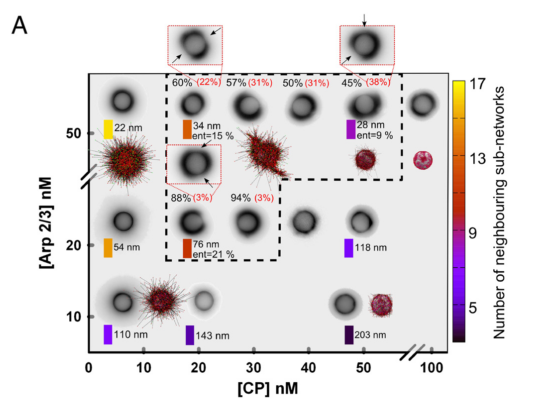
\includegraphics[width=0.700\linewidth]{symmetry-breaking-phase-diagram.png}
\caption{Phase diagram showing symmetry breaking in bead motility assay as a
function of concentration of Arp2/3 and Capping Protein. Symmetry breaking
only occurs inside the area delimited by the dashed line on 4.5 µm beads both
\emph{in vitro} and \emph{in silico}. Experiments are
displayed as inverted fluorescence image. Adapted from {\hyperref[index-latex:kawska2012]{{[}Kawska, Carvalho, Manzi,  et al.  2012{]}}}}\label{index-latex:phase-diag}\end{figure}

In the rest of this chapter we use the bead motility system, but only
consider it during the first phase, where the symmetry breaking has not yet
occurred, or in condition where it should not occur. In particular we will
investigate condition at 25 nM Arp2/3 and concentration of Capping Protein
varying from 0 to 50 nM. As shown in \hyperref[index-latex:phase-diag]{fig  \ref*{index-latex:phase-diag}} this range corresponds to
conditions where no symmetry breaking occurs, but also to conditions in which
symmetry breaking is expected.  It should be noted that unlike
other study that also characterize actin network growing on bead
{\hyperref[index-latex:pujol2012]{{[}Pujol, dRoure, Fermigier, Heuvingh,  2012{]}}}, our system is still dynamically polymerising and thus
changing with time.


\subsection{Liposomes}
\label{index-latex:liposomes}
Beads are used as model biomimetic system that replicates the polymerisation mechanism
happening on the leading edge of cells. Because of their composition and
rigidity, phenomenon observed on beads cannot necessarily reproduce all the interactions and
processes that take place on the cell membrane. Cells are finite compartments with a
limited amount of actin that act on the dynamics of polymerisation.  The fact
that cell size is in the order of the persistence length of actin filaments
also plays a role on the structure of actin networks. Indeed at these scales a
single filament can never reach the length at which it can be considers fully
flexible.

Liposomes are one of the biomimetic systems that are capable of capturing some
interactions between cell membranes. Liposomes are lipid bilayers that imprison
an aqueous compartment and exhibit many characteristics similar to cells.
The inside of liposomes can act as a biochemical reactor of limited size with
the lipid bilayer acting as a separation to the outside, like the cell
membrane. The composition of the lipid layer can be varied in order to reflect
the composition of cell membrane. In particular it is possible to attach
proteins to the liposome membrane. Finally, the size of the liposomes can be
varied, leading to actin networks of size and shape similar to those found in
cells.

It is possible to mimic the cellular actin cortex using liposomes, and especially
its contractility. A crosslinked actin network, can be formed and attached to
the outer leaflet of liposomes, and contractility can be trigged by injecting
molecular motors. The behavior of the system will depend on the attachment
between the reconstituted actin cortex and liposome membrane.  Weak attachment
lead to a favorable rupture of the actin cortex during the increase of tension,
implying a symmetry breaking as in the bead motility system.  In the case of strong
attachment, the liposome actin-cortex will accumulate tension until it has
enough force to crush the supporting lipid layer, thus collapsing the liposome
{\hyperref[index-latex:carvalho2013]{{[}Carvalho, Tsai, Lees,  et al.  2013{]}}},(\hyperref[index-latex:fig-peeling-scheme]{Fig  \ref*{index-latex:fig-peeling-scheme}}). This system also allows the observation
over time giving extra insight into the dynamics of the actin network (\hyperref[index-latex:fig-peeling-3d]{Fig  \ref*{index-latex:fig-peeling-3d}}).
\begin{figure}[htbp]
\centering
\capstart

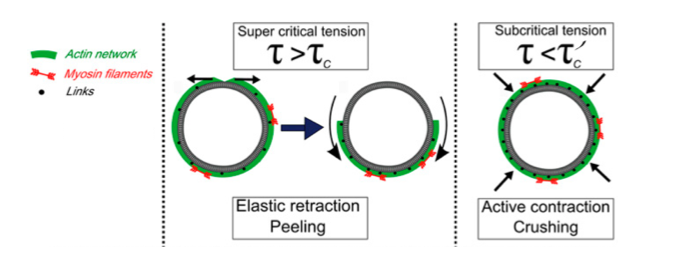
\includegraphics[width=0.800\linewidth]{joel-2-11.png}
\caption{Effect of reconstituted rigid actin cortex attachment to a liposome
membrane under constraints generated by myosin filaments. Under weak attachment
the actin network ruptures thus leading to a ``peeling'' of the actin cortex.
With stronger attachment the actin cortex can sustain higher stresses, until
the underlying liposome ruptures (``Crushing''). Adapted from
{\hyperref[index-latex:carvalho2013]{{[}Carvalho, Tsai, Lees,  et al.  2013{]}}}}\label{index-latex:fig-peeling-scheme}\end{figure}
\begin{figure}[htbp]
\centering
\capstart

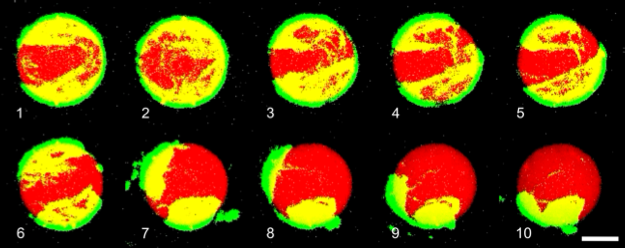
\includegraphics[width=0.900\linewidth]{joel-5-12.png}
\caption{3D reconstruction of an acto-myosin cortex (green actin) peeling off a
liposome (red) over time (1.4 second between frames). The actin cortex
contraction happened after the injection of Myosin II. Scale bar is 5 µm.
Experiments and reconstruction done by Joël Lemière.}\label{index-latex:fig-peeling-3d}\end{figure}


\section{Membrane Physics}
\label{index-latex:membrane-physics}
The cell's plasma membrane is a biological membrane that separates the cell from
its outside environment.  It consists of a lipid bilayer containing
a high numbers of proteins.  A lipid bilayer is formed by two layers of lipids and have a
thickness of a few nm. The classical theoretical description
of these bilayers had been done by W. Helfrich {\hyperref[index-latex:helfrich]{{[}Helfrich,  1973{]}}} in 1973 in a
model based on the elasticity and fluidity of lipid bilayers as well as the
self assembly properties of  lipids.

In the case of close lipid bilayer, the potential energy stored by the
deformation of a lipid bilayer by unit area can be  written as
\phantomsection\label{index-latex:equation-eqa1}\begin{gather}
\begin{split}H = H_{ext} + H_{curv}\end{split}\label{index-latex-eqa1}
\end{gather}
In which \(H_{ext}\) is due to the extension/compression of the membrane,
and \(H_{curv}\) is due to the local curvature of the membrane.

The density of energy cost to extend the membrane \(H_{ext}\) cab be written as a
function  of the elastic area compressibility modulus \(K_a\) and the
relative variation surface of the membrane \(A\) :
\phantomsection\label{index-latex:equation-eqa2}\begin{gather}
\begin{split}H_{ext} = \frac 1 2 K_a \left(\frac{\Delta A}{A}\right)^2\end{split}\label{index-latex-eqa2}
\end{gather}
\(K_a\) express how much energy is required to expand the surface of the
lipid bilayer and is due to the exposition of more hydrophobic surface to water
when expanding it. \(K_a\) is expressed in \(J.m^{-2}\), or \(N/m\)
and is close to twice the surface tension between the lipids and water.

For closed lipid bilayers, the total curvature energy can be expressed as the
sum of the curvature energy \(H_{curv}\) :
\phantomsection\label{index-latex:equation-eqa3}\begin{gather}
\begin{split}H_{cur} = \frac 1 2 \kappa (c_1 + c_2 -c_0)^2\end{split}\label{index-latex-eqa3}
\end{gather}
In which \(kappa\) is the bending modulus of the membrane and \(c_1,c_2\)
are the principal curvatures of the membrane. \(c_0\) is the spontaneous
curvature of the membrane, which is defined as the curvature the membrane would adopt when free of
external constraints.

An important parameter which is introduced in membrane mechanics is the  membrane tension
\(\sigma\) which is the stress associated with an increase in membrane surface.
The tension \(\sigma\) is linked to the energy required to expand the membrane \(H_{ext}\) by :
\phantomsection\label{index-latex:equation-eqa4}\begin{gather}
\begin{split}\sigma &= \frac {\partial H} {\partial \left(\frac{\Delta A}{A}\right)} \\\end{split}\label{index-latex-eqa4}
\end{gather}
i.e.
\phantomsection\label{index-latex:equation-eqa5}\begin{gather}
\begin{split}H_{ext} &= \sigma\left( \frac {\Delta A} A \right)\end{split}\label{index-latex-eqa5}
\end{gather}
In which
\phantomsection\label{index-latex:equation-eqa6a}\begin{gather}
\begin{split}\sigma =  K_a \left( \frac {\Delta A} A \right)\end{split}\label{index-latex-eqa6a}
\end{gather}
Membrane tension is a key parameter as it can be measured in cells, and is one
of the parameters responsible for cell sorting {\hyperref[index-latex:maitre2012]{{[}Maitre, Berthoumieux, Krens,  et al.  2012{]}}}. In particular
between cells, the tension of the couple (membrane+actin cortex) can be
determined by using the contact angle between cell which is the angle between
interfaces as defined in \hyperref[index-latex:fig-tension-cell]{figure  \ref*{index-latex:fig-tension-cell}}.
\begin{figure}[htbp]
\centering
\capstart

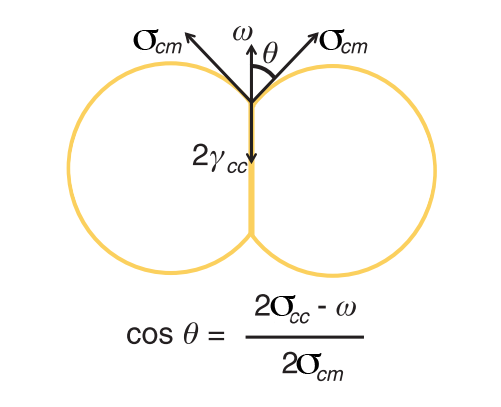
\includegraphics[width=0.400\linewidth]{Cell-Surface-tension.png}
\caption{Surface tension govern doublet shape,  adapted from {\hyperref[index-latex:maitre2012]{{[}Maitre, Berthoumieux, Krens,  et al.  2012{]}}}.
The equilibrium of forces on the contact line govern the angle of contact
\(2.\theta\). \(\omega\) corresponds to the adhesion tension between
the two cells, \(\sigma_{cm}\) correspond to the tension between
the cell and the medium, \(\sigma_{cc}\) correspond to the cortex
tension between the two cells.}\label{index-latex:fig-tension-cell}\end{figure}

In a later part, we use a reconstituted biomimetic system made of liposomes. The
injection of myosin motors changes the tension of the acto-myosin cortex
attached to a membrane. By determining the geometrical parameters of this
system, and in particular the evolution of the contact angle with time, we are
able to measure the variation of tension of the acto-myosin cortex due to contraction by
molecular motors.


\section{Actin networks as viscoelastic material}
\label{index-latex:viscoelastic}\label{index-latex:actin-networks-as-viscoelastic-material}
We have seen previously that while polymerising, G-actin assembles into F-actin
filaments. The stiffness of filaments can be measured by a characteristic number
called the persistence length (\(l_p\)). More precisely, the
persistence length characterizes the average loss of correlation between the
tangent along the considered polymer. With \(s\) the curvilinear abscissae along the polymer,
and \(\Theta_{(x,y)}\) the angle between the two tangent at two different abscissae (\hyperref[index-latex:fig-persistence-length]{Fig  \ref*{index-latex:fig-persistence-length}}):
\phantomsection\label{index-latex:equation-eqa6}\begin{gather}
\begin{split}\left<\Theta_{(s,s+l)}\right> = exp\left(\frac{-l}{l_p}\right)\end{split}\label{index-latex-eqa6}
\end{gather}
For actin filaments, the
persistence length is in the order of 10 µm {\hyperref[index-latex:isambert1995]{{[}Isambert, Venier, Maggs,  et al.  1995{]}}}. This means
that for scales much smaller, the actin filament can be considered as rigid.
This is the case in the cell cortex where the meshwork has a typical size smaller than 250 nm. In
the other extreme, at length scale much bigger than \(l_p\), filaments can
be considered as flexible. While in typical cells, the filament length is
rarely much bigger than the persistence length of actin, \emph{Xenopus} eggs can be
as big as 1 mm, so hundreds fold the actin persistence length.
Still for the majority of cells, the typical size we are interested in
is about the persistence length of an actin filament, making it neither purely
rigid nor completely flexible.
\begin{figure}[htbp]
\centering
\capstart

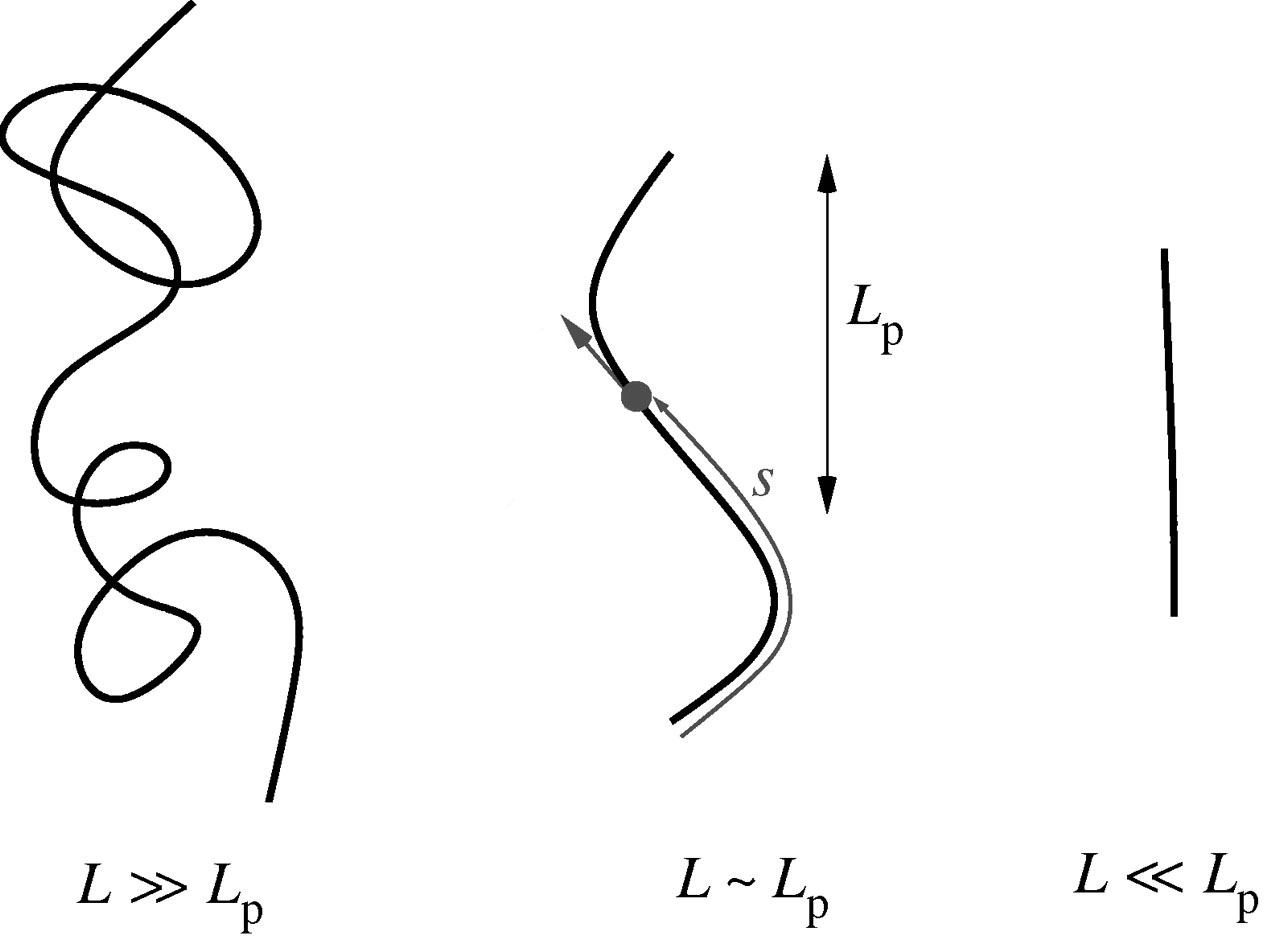
\includegraphics[width=0.600\linewidth]{F2_large.jpg}
\caption{Schematic of polymers with length respectively big compared to the persistence
length (A), in the order of the persistence length (B) and small compared
to persistence length (C), \(s\) as defined on (B) is the \emph{curvilinear
abscissae}, that is to say the distance between two points of the polymer
measured by ``following'' the polymer. Adapted from {\hyperref[index-latex:liverpool2006]{{[}Liverpool,  2006{]}}}}\label{index-latex:fig-persistence-length}\end{figure}

For the above reasons, actin solutions are often compared to semi-flexible
polymers, and models that predict the behavior of actin networks often take
foundation on polymers physics {\hyperref[index-latex:morse1998b]{{[}Morse,  1998b{]}}} {\hyperref[index-latex:morse1998a]{{[}Morse,  1998a{]}}}. Still, if
theses models rely on local microscopic parameters, experimental methods only
have access to bulk properties of the studied material, and it is from theses
properties, and through the models that we can deduce possible values for the
microscopic models {\hyperref[index-latex:mackintosh1995]{{[}MacKintosh, Kas, Janmey,  1995{]}}}.


\subsection{Elastics Modulus}
\label{index-latex:elastics-modulus}\label{index-latex:elastic-modulus}
The elastics moduli are probably the easiest to understand. They are
a characteristic of how a material will deform non-permanently under an applied
force. The stiffer something is the higher its elastics moduli will be. There
are two specific elastic moduli of interest in this
manuscript, \emph{Young's Modulus} and \emph{shear modulus}. The first one describes how a material will react to compression or extension, while the
second describes how a material resists  shearing. For isotropic and homogeneous
materials, the Young's modulus (E) and the shear models (G) are related
by the Poisson ratio (\(\nu\)):
\phantomsection\label{index-latex:equation-eqa7}\begin{gather}
\begin{split}G = \frac{E}{2(1+\nu)}\end{split}\label{index-latex-eqa7}
\end{gather}
Both G and E units are homogeneous to \(N/m^2\) or
\(Pa\).  It is instructive to have an idea of the order of magnitude of a
few usual materials. Aluminum will have an elastic modulus \(G_{Al}\simeq
70~GPa\) while rubber will be more in the order of \(G_{rubber}\simeq
0.1~GPa\). The elastic modulus of muscle cell is in the order of
\(G_{muscle} \sim 10~kPa\) and brain tissues around \(G_{brain} \sim
0.1~\text{to}~1~kPa\) {\hyperref[index-latex:engler2006]{{[}Engler, Sen, Sweeney, Discher,  2006{]}}}.

A  more formal definition of the Young's modulus, is the ratio between
the stress \(\sigma\) along the direction of the deformation and the relative deformation \(\epsilon\).
\phantomsection\label{index-latex:equation-eqa8}\begin{gather}
\begin{split}E &= \frac{\sigma}{\epsilon} \\
  & = \frac{   F/S }{   \Delta L / L_0        }\end{split}\label{index-latex-eqa8}
\end{gather}
In which \(F\) is the applied force, \(S\) is the cross section of the
material, \(\Delta L\) is the elongation and \(L_0\) is the initial
length of the considered material.  (\hyperref[index-latex:fym]{Figure  \ref*{index-latex:fym}} A):
\begin{figure}[htbp]
\centering
\capstart

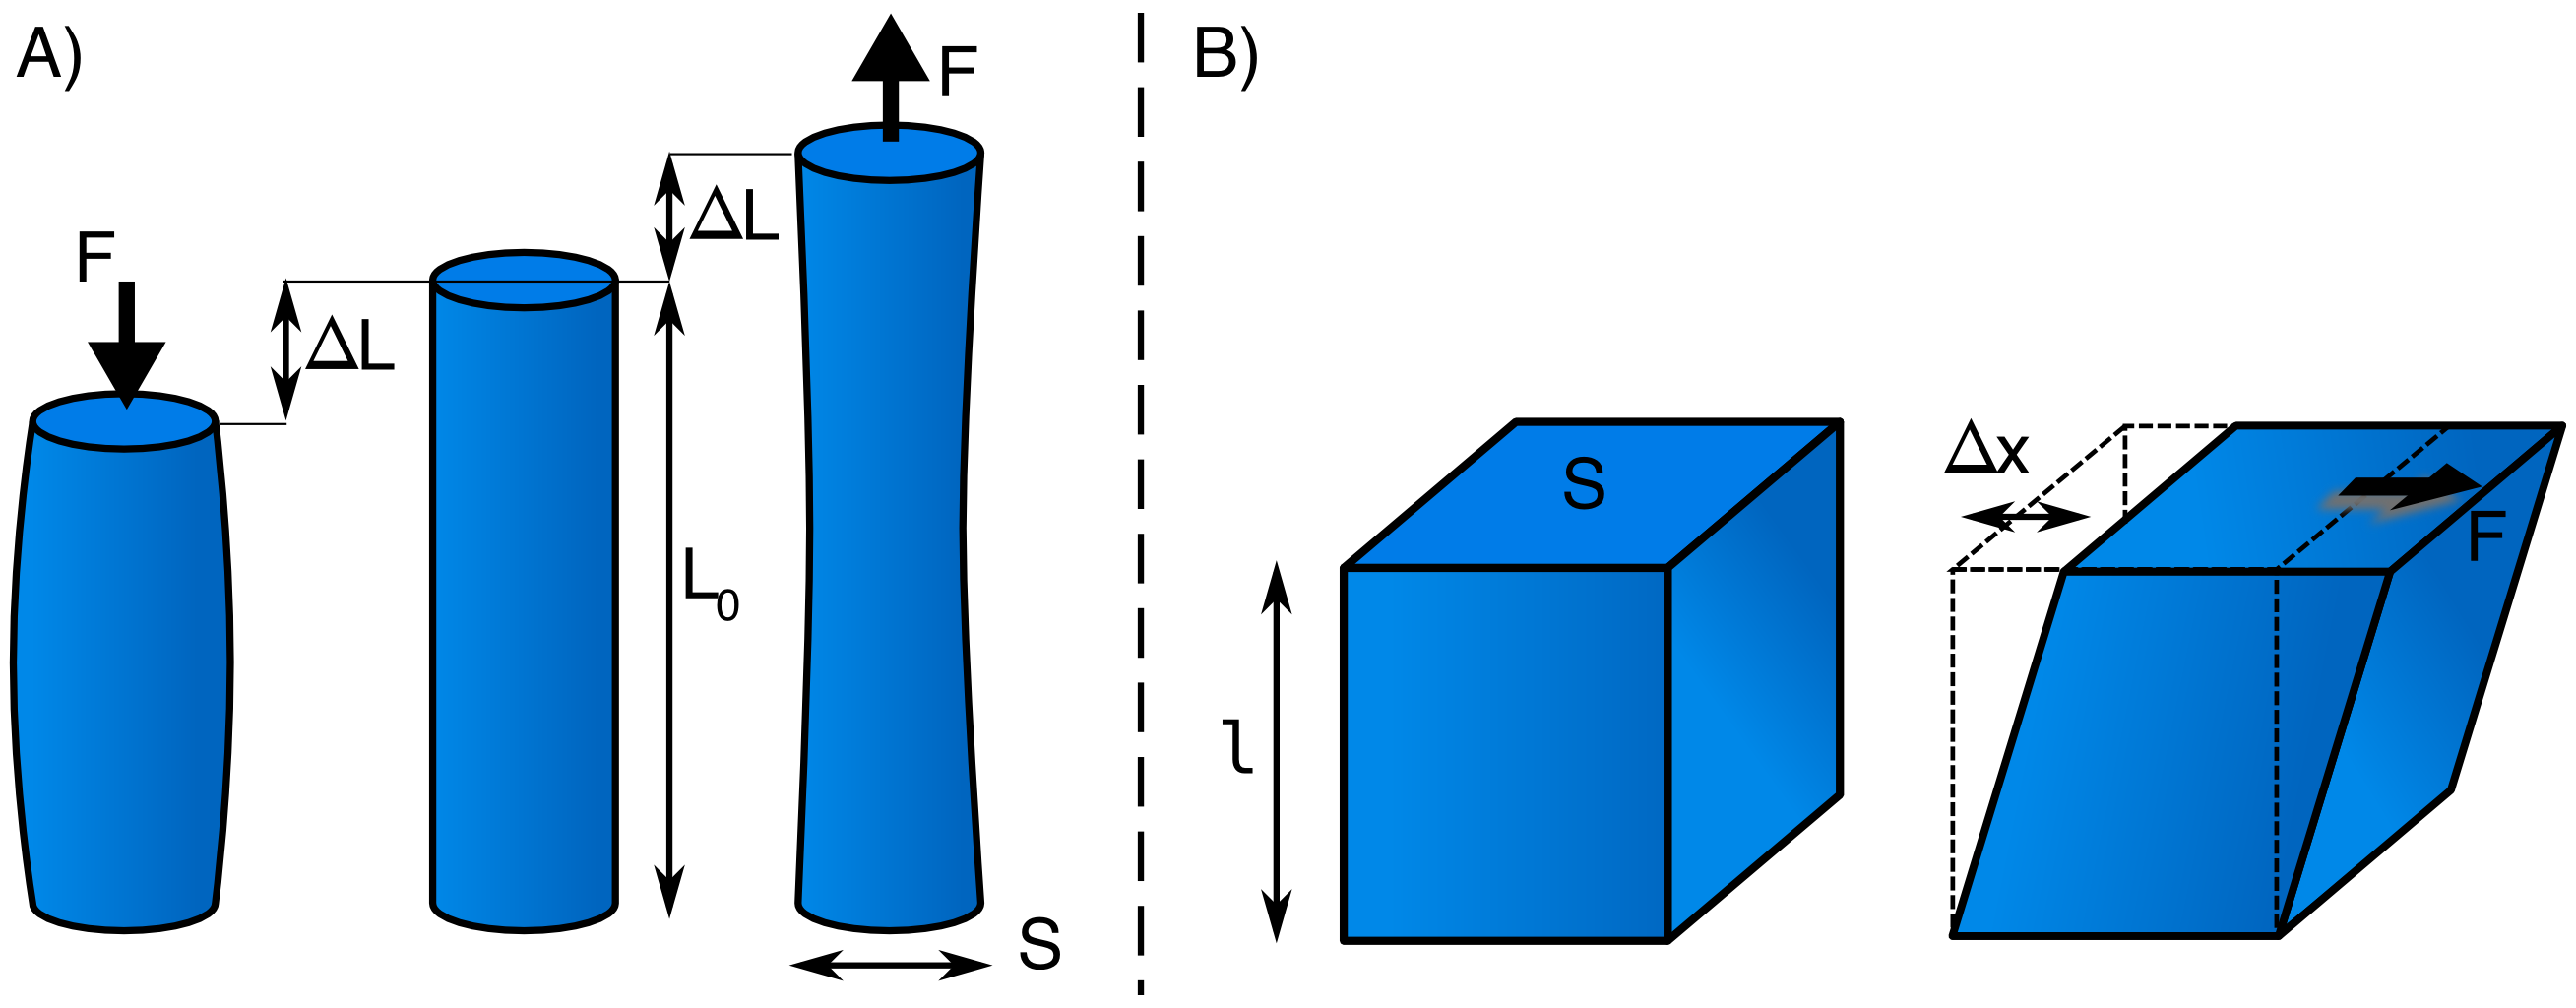
\includegraphics[width=0.800\linewidth]{youngm.png}
\caption{Schematic of the Young Modulus definition. F, force applied to sample, S
surface of cross section when uncompressed, \(L_0\), length when no load
applied. For both compression and extension, in the regime of small
deformation, the relative change of length is proportional to the applied
force. Here, the material can be seen to expand/contract in the direction
orthogonal to the direction of application of the force, in the case of an
incompressible material (\(\nu \neq 0.5\)) this can be seen as the
conservation of volume of the material.}\label{index-latex:fym}\end{figure}

The shear modulus is defined for a deformation parallel to the surface on which it is applied :
\phantomsection\label{index-latex:equation-eqa9}\begin{gather}
\begin{split}G &= \frac{\tau_{xy}}{\gamma_{xy}} \\
  & = \frac{   F/S }{   \Delta x / l        }\end{split}\label{index-latex-eqa9}
\end{gather}
In which \(\tau_{xy}\) is the shear stress, \(\gamma_{xy}\) is the shear strain, \(F\) is the applied force
on the cross section of the material \(S\). \(l\) is the thickness of the material and \(\Delta x\) is the
transverse displacement (\hyperref[index-latex:fym]{Fig  \ref*{index-latex:fym}} B).

Other characteristic numbers can also be defined, such as the bulk modulus. In the case of isotropic
elastic materials, only two of those parameter are required to completely define
the properties of the material.


\subsection{Poisson Ratio}
\label{index-latex:poisson-ratio}
We have seen that the shear modulus is linked to the Young modulus using
the Poisson ratio.  The Poisson ration is another characteristic of a material
that defines how much a material will compress/expand in the directions
orthogonal to its elongation.

The Poisson ratio is the negative ratio of transverse to axial strain :
\phantomsection\label{index-latex:equation-eqa10}\begin{gather}
\begin{split}\nu = - \frac{
    d \epsilon_{trans}
}{
    d \epsilon_{axial}
}\end{split}\label{index-latex-eqa10}
\end{gather}
In which \(\epsilon_{axial}\) is the relative deformation along one of the
axis of compression/elongation and \(\epsilon_{trans}\) correspond to the
relative deformation along an axis orthogonal to the axis of deformation.

Having volume conservation during compression or elongation require
a Poisson ratio of \emph{0.5}. Such values have been found in bulk measurements of
actin network at concentrations 21.5 µM of actin {\hyperref[index-latex:gardel2003]{{[}Gardel, Valentine, Crocker,  et al.  2003{]}}}. Materials with a Poisson ratio of \emph{0.5} are
said to be incompressible. A Poisson ratio lower \emph{0.5} correspond to material
expanding less than incompressible materials, some cell and tissues are known to
have Poisson ratio lower than 0.5 {\hyperref[index-latex:mahaffy2004]{{[}Mahaffy, Park, Gerde,  et al.  2004{]}}}. Another critical value
is 0, at which the material only expand or contract in the direction of the
main stress.

Materials with a Poisson ratio superior to 0.5 would show a bigger
deformation in the orthogonal direction than incompressible material, leading
to a global increase of volume if compressed.


\subsection{Viscosity}
\label{index-latex:viscosity}
Like elasticity, viscosity is something tangible we are used to work with in
everyday life. The more viscous a material is the more difficult it is to move
something in it at high speed. And indeed, viscosity is the pendant of the elastic
modulus but considering forces induced by the deformation rate instead of displacement.
\phantomsection\label{index-latex:equation-eqa12}\begin{gather}
\begin{split}\frac{F}{S} &= \tau_{xy} \\
            &= \eta \frac{\partial v}{\partial z}\end{split}\label{index-latex-eqa12}
\end{gather}
In which \(\tau_{xy}\) is the shear stress, \(F\) is the force exerted
on the surface \(S\). \(\eta\) is the viscosity, and is expressed in
\(Pa.s\), \(v\) is the deformation rate along the direction \(z\) .

At room temperature water has a viscosity of around 1 mPa.s, and honey of 10 Pa.s. The consideration of viscosity in problems will
often depend on the timescale and deformation rate. At short
timescale tissue often behaves elastic, whereas at long timescale the effect
of viscosity will be seen {\hyperref[index-latex:thoumine1997]{{[}Thoumine, Ott,  1997{]}}}. In actin networks, the effect of
viscosity at short time scale can be similar to elasticity {\hyperref[index-latex:gardel2003]{{[}Gardel, Valentine, Crocker,  et al.  2003{]}}}.


\subsection{Viscoelasticity}
\label{index-latex:viscoelasticity}
Typically, no material is purely elastic or purely viscous. While glaciers
seem purely solid at the time scale of a few days, observation on longer time
scale ranging from month to years show that ice is not only a
solid but can also flow. Of course ice in its solid form is not the only
material which is both solid and viscous. In order to describe such
behavior one can use the theory of viscoelastic materials.  A number of models have
been and are still developed to describe viscoelastic behavior. The
Kelvin-Voigt and Maxwell models are two of the simpler ones (\hyperref[index-latex:fig-mkv]{Fig  \ref*{index-latex:fig-mkv}}). A thought
experiment to understand each of these model is to put a spring and a dash pot
in parallel or series. Such model systems exhibit viscoelastic behavior.
\begin{figure}[htbp]
\centering
\capstart

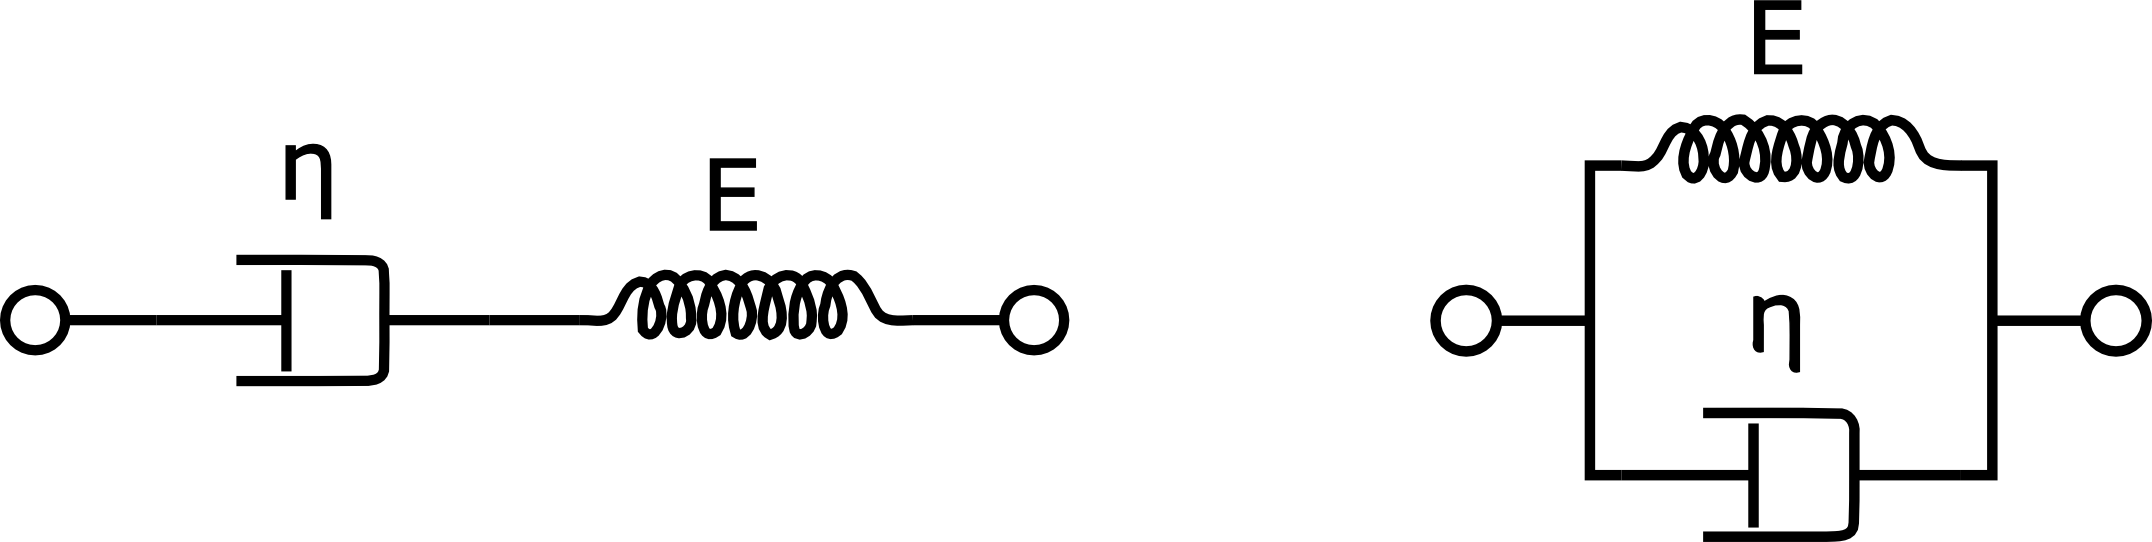
\includegraphics[width=0.700\linewidth]{MKV.png}
\caption{Maxwell model schematic on the left and Kelvin-Voigt model on the right.
Both are simple approaches to express the properties of a viscoelastic
solid. The response to a creep compliance will differ in both case. The Maxwell
model will mostly behave like a fluid with viscosity \(\eta\) after a
long time, where the Kelvin-Voigt model will mostly reflect the elastic
components at constant stress exerted. (Schematic in Public Domain, adapted
from Wikimedia).}\label{index-latex:fig-mkv}\end{figure}

The idea for more complex models is similar, where any material can be seen like an
(infinite) combination of springs (for elasticity), and dash-pots, (for viscosity).

Theory of viscoelastic materials explains the mechanical properties of a system by
using a single function which is the viscoelasticity of a material. This can
be done by describing \(E\) as a relaxation modulus depending on time.  In
the case of a linear system we can express the strain on the material at a given
time as a function of its history :
\phantomsection\label{index-latex:equation-strain}\begin{gather}
\begin{split}\sigma (t)  = \int_0^t E(t-\tau) \frac{du}{d\tau} d\tau\end{split}\label{index-latex-strain}
\end{gather}
In which \(\sigma(t)\) is the time dependent stress, and \(u(t)\) is
the known strain.

Using rheology, it is common to measure the properties of a material using a
sinusoidal strain of known amplitude \(u_0\) and frequency \(f =
\omega/ 2.\pi\) : \(u(t) = u_0.cos(\omega t)\), which also implies a
sinusoidal strain rate. Using the complex notation \(\dot u = u_0 i\omega
e^{i\omega t}\) in equation \eqref{index-latex-strain}, and operating the change of variable \(t-\tau \to t'\)  leads to :
\phantomsection\label{index-latex:equation-eqa13}\begin{gather}
\begin{split}\sigma(t) = u_0\int_0^\infty E(t') i\omega e^{i\omega(t-t')}dt'\end{split}\label{index-latex-eqa13}
\end{gather}
By factoring out the time dependent part, the rest can be rewritten as two integrals with respectively a real and imaginary prefactors :
\phantomsection\label{index-latex:equation-eqt}\begin{gather}
\begin{split}\sigma(t) = u_0e^{i\omega t}\times\left(
          \omega \int_0^\infty E(t')  sin(\omega t) dt'
          +
        i \omega \int_0^\infty E(t') cos(\omega t) dt'
\right)\end{split}\label{index-latex-eqt}
\end{gather}
The two integrals in brackets only depend on the pulsation \(\omega\) and the properties of the considered material.
They are both in factors of the complex strain \(u(t) = u_0 e^{i\omega t}\)
We thus define the storage modlus of the material as the real part of (\eqref{index-latex-eqt} in bracket) \(E'\) :
\phantomsection\label{index-latex:equation-eqa14}\begin{gather}
\begin{split}E'(\omega) =  \omega \int_0^\infty E(t')  sin(\omega t) dt'\end{split}\label{index-latex-eqa14}
\end{gather}
And the loss modulus as the imaginary part of (\eqref{index-latex-eqt} in bracket)
\phantomsection\label{index-latex:equation-eqa15}\begin{gather}
\begin{split}E"(\omega) =  \omega \int_0^\infty E(t')  cos(\omega t) dt'\end{split}\label{index-latex-eqa15}
\end{gather}
And define the complex frequency dependent Young's modulus as :
\phantomsection\label{index-latex:equation-eqa16}\begin{gather}
\begin{split}E^*(\omega) = E'(\omega) + i.E"(\omega)\end{split}\label{index-latex-eqa16}
\end{gather}
Thus we can write \eqref{index-latex-eqt} as :
\phantomsection\label{index-latex:equation-eqa17}\begin{gather}
\begin{split}\sigma(t) = E^*(\omega).u(t)\end{split}\label{index-latex-eqa17}
\end{gather}
In this representation of \(E^*(\omega)\), the real part will correspond to
the elastic response of the material (in-phase response
under oscillatory strain) and the imaginary part corresponds to the viscous response
of the system (out of phase under sinusoidal strain). The complete knowledge of
\(E^*(\omega)\) at all frequency completely characterizes the material.

Models for actin networks have been extensively studied as viscoelastic material
both theoretically {\hyperref[index-latex:morse1998a]{{[}Morse,  1998a{]}}}, {\hyperref[index-latex:kruse2005]{{[}Kruse, Joanny, Julicher,  et al.  2005{]}}} , and  experimentally
{\hyperref[index-latex:mizuno2007]{{[}Mizuno, Tardin, Schmidt, Mackintosh,  2007{]}}}.  Actin networks have also been shown to exhibit linear
characteristic behavior, but also and non-linear behaviour  in a certain concentration ranges has been observed {\hyperref[index-latex:yao2011]{{[}Yao, Becker, Broedersz,  et al.  2011{]}}}, {\hyperref[index-latex:gardel2003]{{[}Gardel, Valentine, Crocker,  et al.  2003{]}}}.

The actin networks we will study hereafter are in the condition where linear
behavior is expected, thus we will use the viscoelastic theory to interpret the
relation stress/strain observed in order to determine the mechanical properties
of the formed actin gels.


\section{Optical tweezer}
\label{index-latex:optical-tweezer}\label{index-latex:id77}
Optical tweezers, or optical traps are a technique that allows to trap objects
near the focal plane of a microscope at the focal point of a high power laser.
It is a versatile technique that allows to trap both fabricated objects and
part of living cell. Optical traps typically allow to apply forces up to a few tenth of
pico Newton.

To understand that light can trap an object, it is instructive to keep in mind
that despite having no mass, photons carry momentum, and as for any massive
object, changing the trajectory requires a force.  According to Newton's third
law, when applying a force via a photon on an object, the object will in turn
exert the opposite force on the photon, thus changing the trajectory of the
photon. If a photon changes trajectory in a material, the material has to apply a
force on the photon (\hyperref[index-latex:setup]{Fig  \ref*{index-latex:setup}}), meaning that the photon also applies a force on the
material. In particular, the higher the refractive index of a material, the
more light beams are deviated, and hence the more photons apply forces on
material.

In particular, it can be shown that objects with a higher refractive
index than the surrounding medium are attracted towards higher light intensities
(\hyperref[index-latex:setup]{Fig  \ref*{index-latex:setup}}).  In parallel laser beams, with a Gaussian intensity
profile, this will lead to the object being attracted towards the center of the
beam.

In addition to the lateral trapping, the laser focus leads to
another intensity gradient along the direction of propagation of the
beam, the intensity being at its maximum at the laser waist.

A laser coupled into a microscope objective then acts as a three dimensional
potential that traps particles similar to a tweezer. Usually the trapping in
parallel to the direction of the laser is only about half as strong if compared to the trapping in the
lateral direction.
\begin{figure}[htbp]
\centering
\capstart

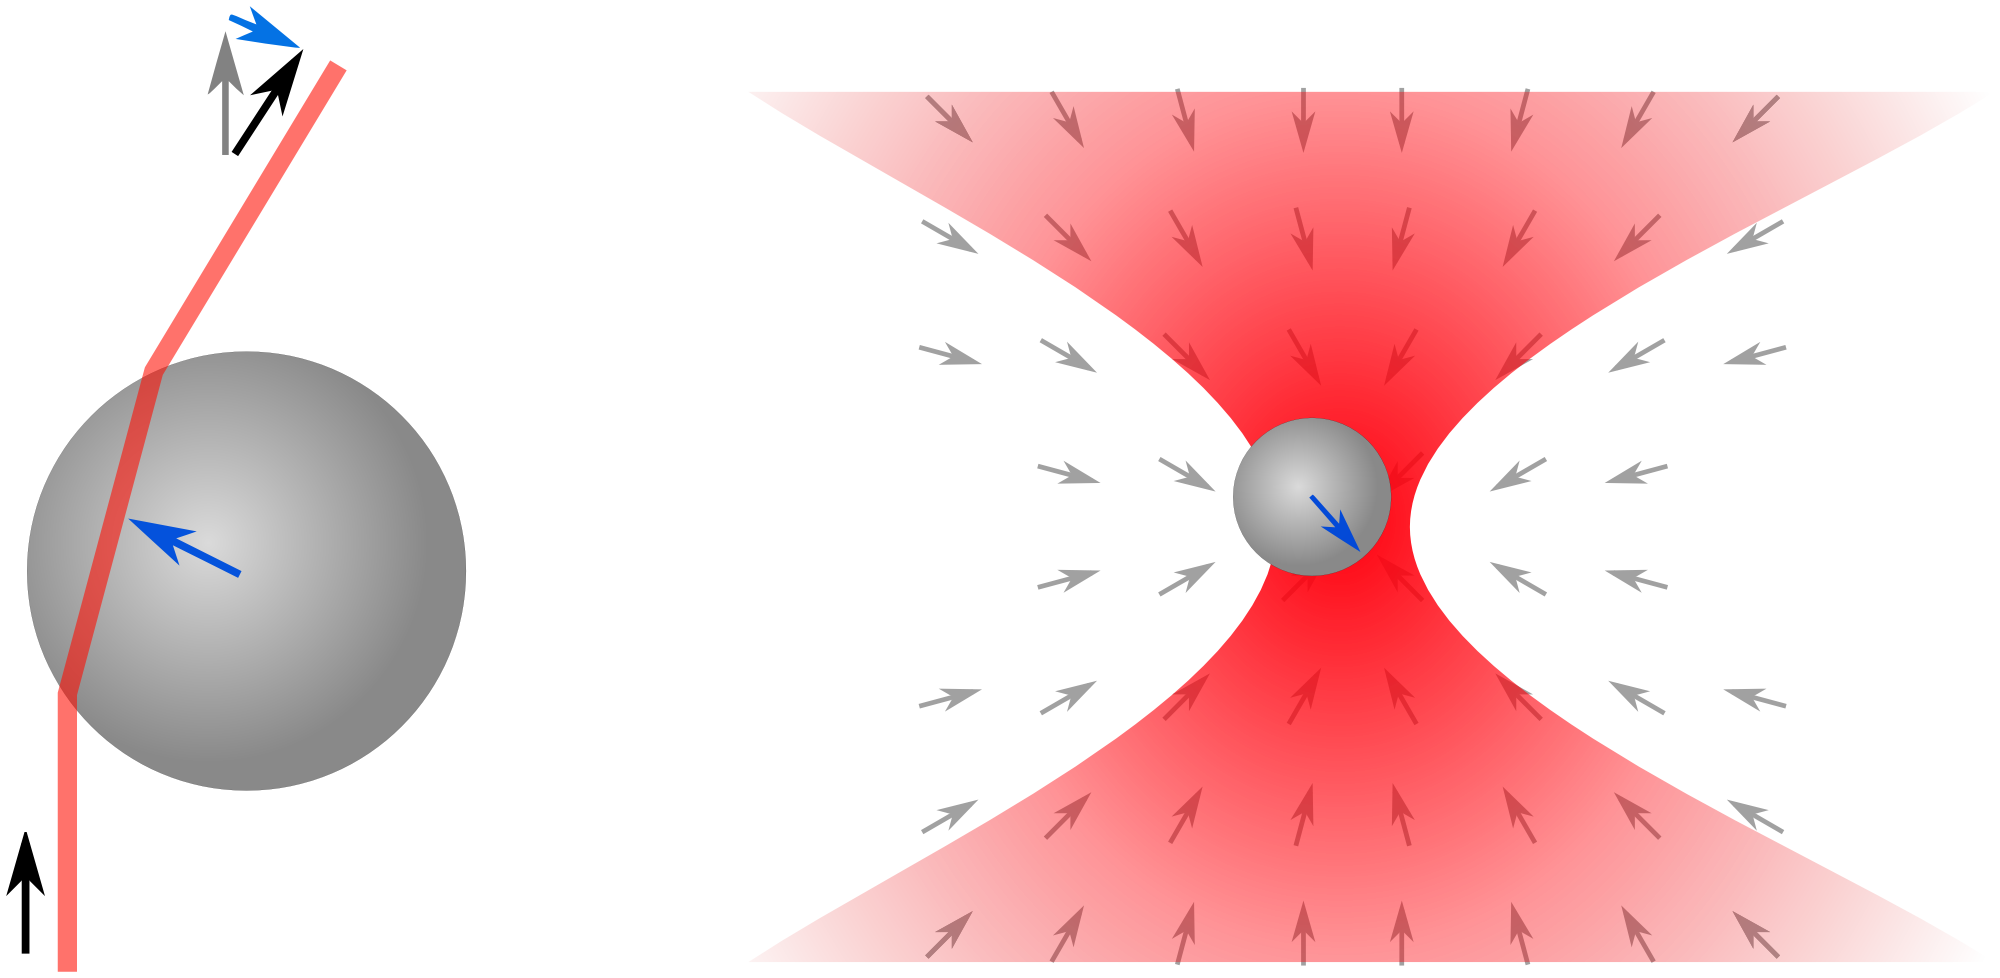
\includegraphics[width=0.700\linewidth]{ot1.png}
\caption{Light deflected by a transparent bead changes the momentum of light, so the
light is exerting a force on the bead. The bead will be attracted towards
the highest intensity.  For a focused laser beam, the bead will be attracted
near the focus of the laser.}\label{index-latex:setup}\end{figure}

One of the qualities of optical traps is that in principle, multiple traps can be
obtained. A simple method to generate two traps is to split the incoming light
into two orthogonally polarized independent beams.  Instead of sharing the
laser power between the different traps by using polarisation, one can use what
is known as multiplexing by time sharing. This is achieved by switching the laser rapidly
between different positions at a speed much faster than the diffusion of the particle. By this method
it is possible to virtually achieve multiple traps on the same
sample.

In this work we use a multiplexed system, where the rapid switching is achieved using Accousto Optic Deflectors
(aka AODs).  An AOD consists of a crystal in which a high frequency
sound-wave propagates perpendicular to the incoming laser beam. This sound-wave generates local changes in the
refractive index of the material which act as a diffraction grating. In
the right conditions, a laser passing through the crystal will
be deflected by this grating under the Bragg angle.

In practice, rapidly controlling the frequency and amplitude of the sound wave
in the crystal, allows direct adjustment of laser deflection and hence the
trap position.  Using AODs also has the advantage of controlling not only
of the number and position of multiple traps, but also the individual power
allocated to each trap and hence the stiffness of each trap.
\begin{figure}[htbp]
\centering
\capstart

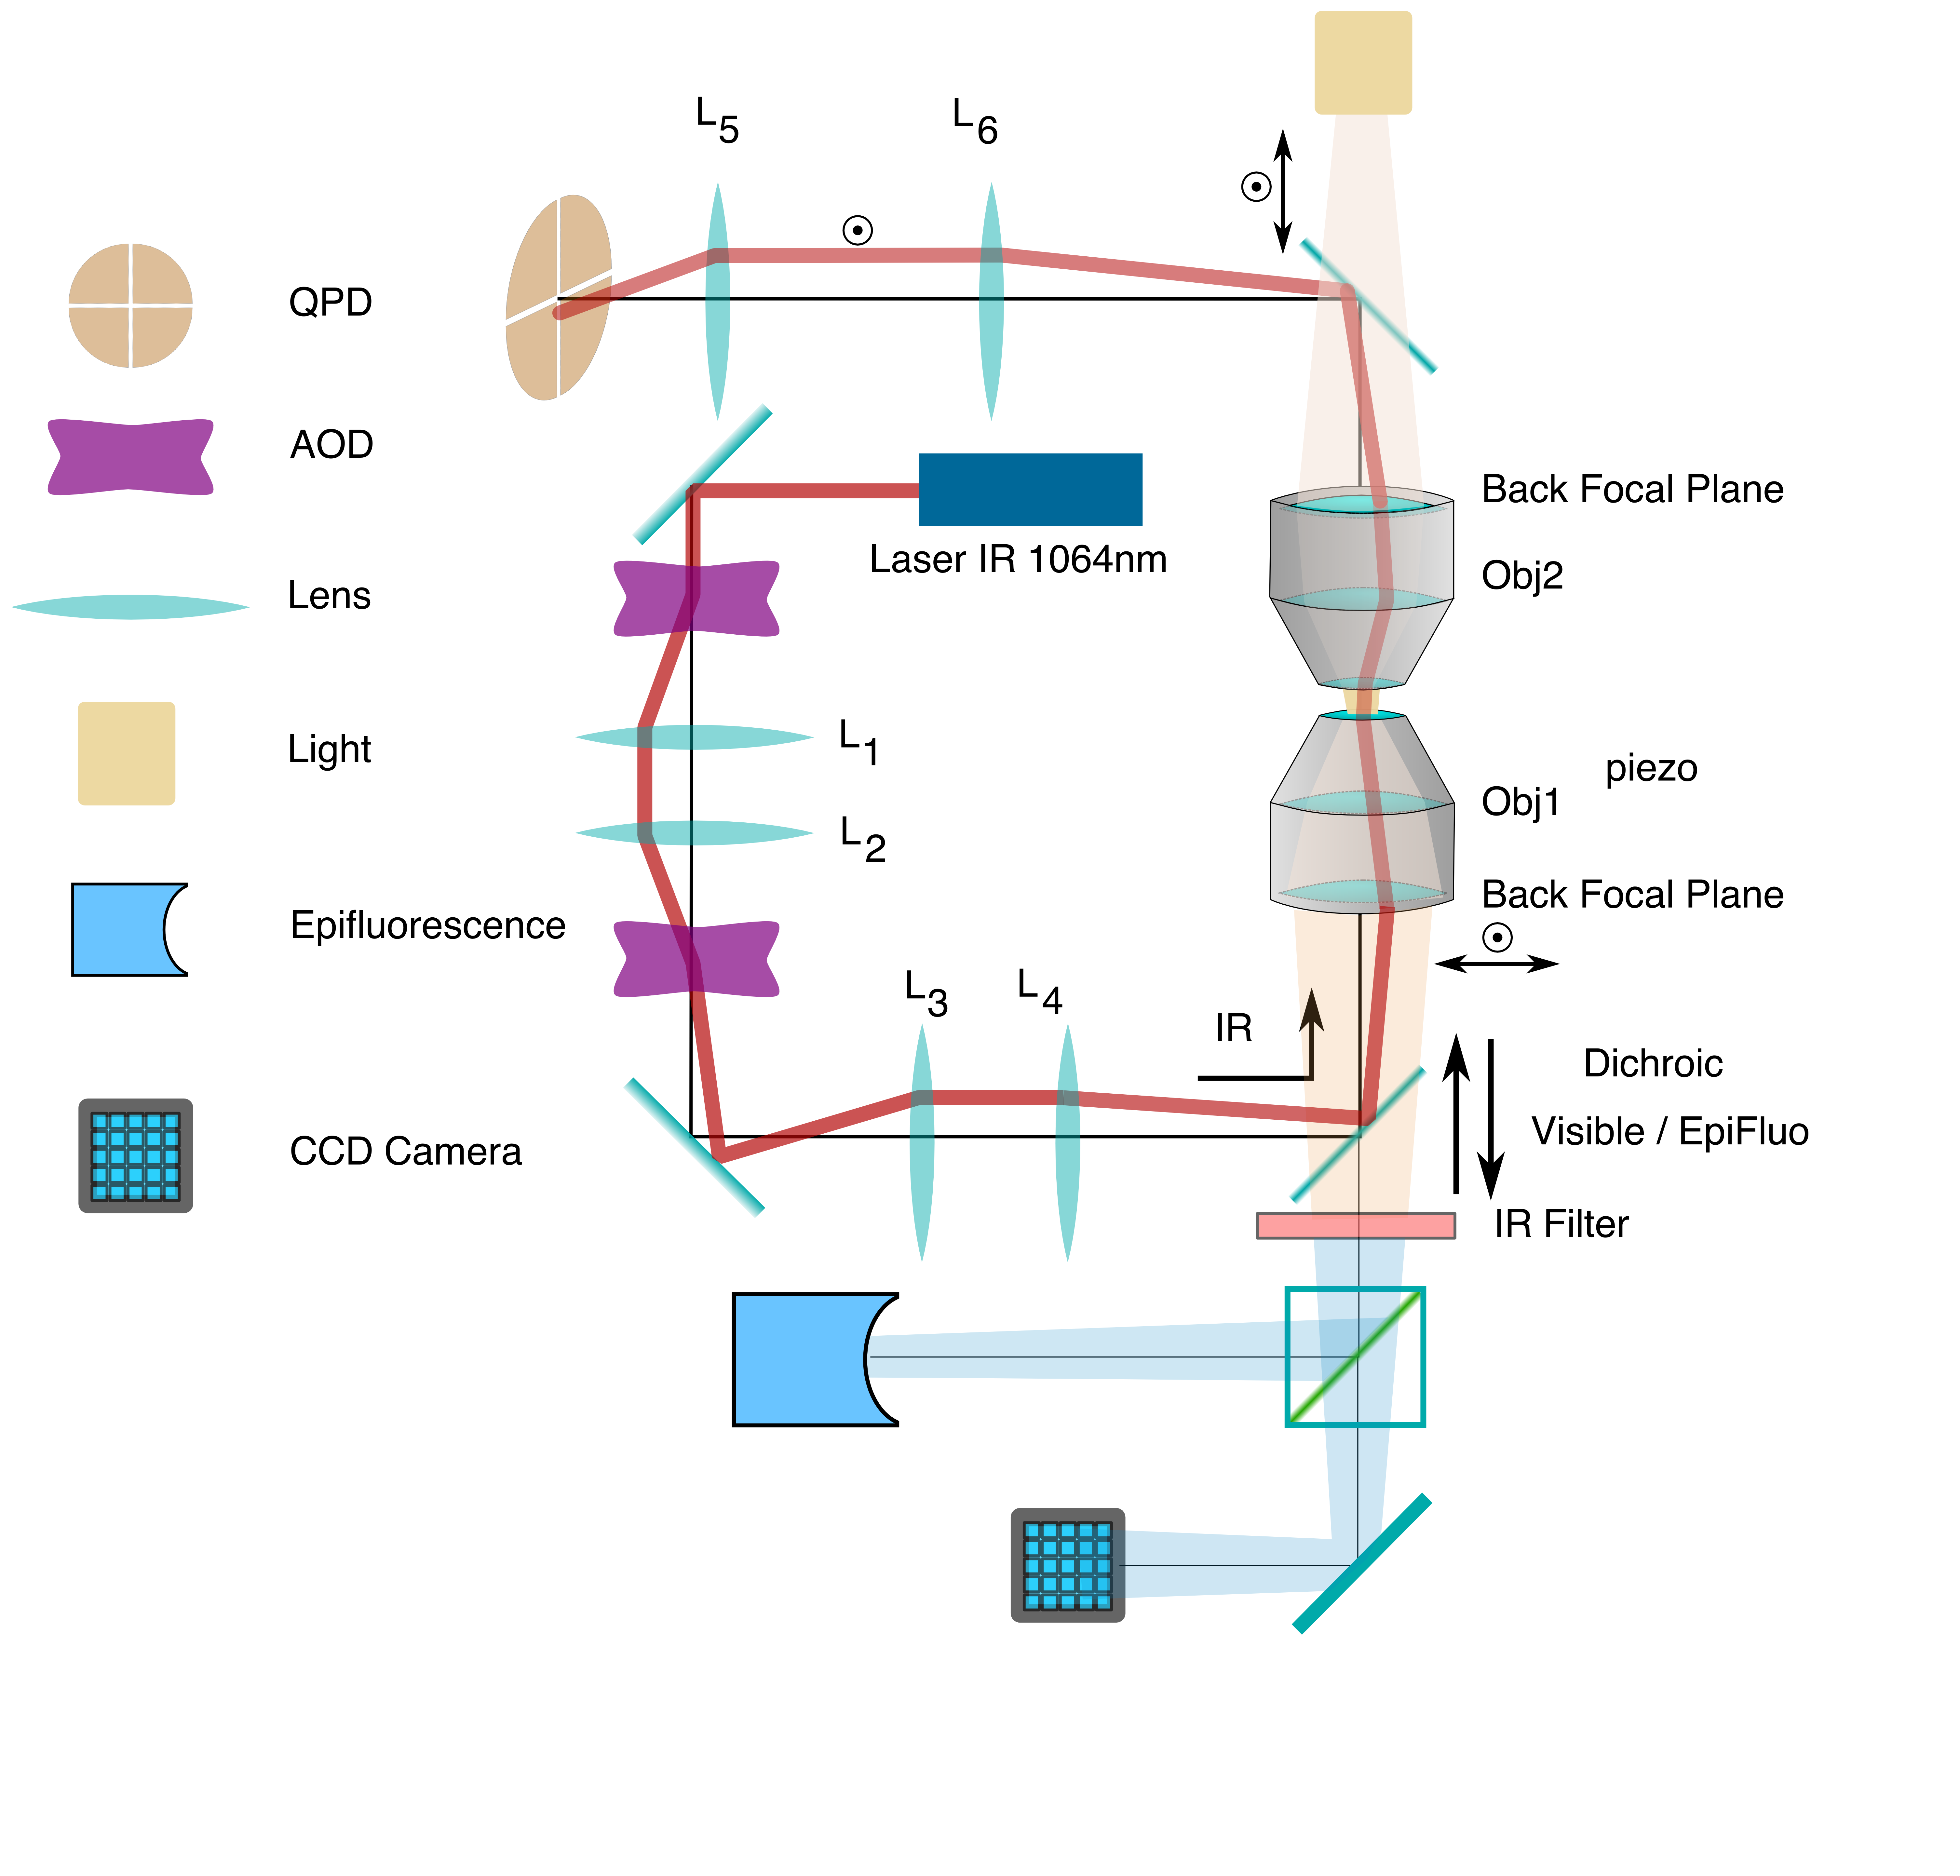
\includegraphics[width=0.900\linewidth]{setup-plus-1.png}
\caption{A schematic of  setup used. The following elements can be distinguished. An
1064nm laser is used for trapping. It first passes through two AODs that
move the position of the trap in the X  and Y direction.  The first couple
of lenses (L1,L2) between AODs assure that AODs are in conjugated planes.
The second pair of lens (L3,L4) image the AODs plane in back-focal plane
of the first objective.
Thus a change of angle of the light beam induce by the AOD
result in a  change of position of the trap.  The trapping light
is collected by a second objective, and illuminates a quadrant photodiode
(QPD) conjugated to the back focal plane of the collecting objective. By
construction QPD and AODs should be conjugated, so deviation of the light
beam induced by one of the AODs is not supposed to induce any change of
position of the laser spot on the QPD. Additional dichroics mirrors allow to
use bright field and epifluorescence simultaneously optical
tweezer.}\label{index-latex:ots}\end{figure}

A schematic of the optical setup that can be used to trap beads in the focal
plane on the microscope can be found in \hyperref[index-latex:ots]{figure  \ref*{index-latex:ots}}. The scheme also
contains the detection part of the setup that is used to measure the force
exerted on each bead, technique which is explained on following part.


\subsection{Determination of trapping forces and bead displacement}
\label{index-latex:determination-of-trapping-forces-and-bead-displacement}
In addition to allowing the objects to be hold in place, the use of a QDP
(Quadrant Photo Diode, a precise position detector) with optical traps
has the advantaged to acquire high frequency quantitative measurement of
the displacement and force exerted on an object.  Indeed, when the trapped
particle is not in the trap center, the laser applies a force on the object.
Reciprocally, the object applies the opposite force on the light beam, thus
deflecting the light beam.  Using optics and lenses correctly placed on the
Fourier plane of the sample, it is hence possible to translate this change of
orientation of the light  beam into a displacement of a light spot onto a photo
detector with hight sensitivity to applied forces.

Through careful calibration of the trap, that give the force/displacement
relationship, {\hyperref[index-latex:jahnel2011]{{[}Jahnel, Behrndt, Jannasch,  et al.  2011{]}}}, {\hyperref[index-latex:vermeulen2006]{{[}Vermeulen, vMameren, Stienen,  et al.  2006{]}}}, one can then also
recover the displacement of the sample inside the optical trap.

Using optical tweezer to not only hold a particle in position, but also to get
quantitative measurement of its displacement and the force exerted require to
calibrated each probe particle. Polystyrene beads are common artificial probes
used to achieve such a goal.

The use of polystyrene bead has multiple advantages. First, one
can obtain mono-dispersed beads leading to reproducible and predictable trap
stiffness. Secondly, theory can predict the shape of
the potential felt by such a bead in a Gaussian beam {\hyperref[index-latex:nieminen2007]{{[}Nieminen, Knoner, Heckenberg, RubinszteinDunlop,  2007{]}}}.

The third advantage is that beads can be functionalized, allowing specific
interaction to be controlled, both \emph{in vitro} and \emph{in vivo}. Of course, the
calibration is essential for the correct measurement of mechanical property of
different system, and the choice of the bead diameter have impact both on
biological side and in the physics of the measurement.
\phantomsection\label{index-latex:part2}

\chapter{Materials and Methods}
\label{index-latex:part2}\label{index-latex::doc}\label{index-latex:m-et-m}\label{index-latex:materials-and-methods}

\section{Buffers}
\label{index-latex:buffers}

\subsection{G-Buffer}
\label{index-latex:g-buffer}
G-Buffer is used to conserve actin in the monomeric form. Actin is diluted in
G-Buffer and kept on ice for at least 12 hours before further use. G-buffer is
aliquoted and stored at -20°C. For weekly use or is thawed and conserved on ice for up to a week. G-buffer is never
refrozen. pH is adjusted between 7 and 8.

Composition of G-Buffer:
\begin{itemize}
\item {} 
0.2 mM \(CaCl_2\)

\item {} 
0.5 mM DTT (Dithiothreitol, or (2S,3S)-1,4-bis(sulfanyl)butane-2,3-diol)

\item {} 
2.0 mM Tris (tris(hydroxymethyl)aminomethane or 2-Amino-2-hydroxymethyl-propan)

\item {} 
0.2 µM ATP (Adenosine triphosphate)

\end{itemize}


\subsection{Polymerisation Buffer}
\label{index-latex:polymerisation-buffer}
Polymerisation buffer or X-Buffer is used for polymerisation of actin gels on
beads  as well as bead dilution and cleaning buffer.  It is aliquoted and conserved at
-20°C. During experiments it is stored on ice for up to a week. X-Buffer is never
refrozen.

Composition of X-Buffer :
\begin{itemize}
\item {} 
10 mM Hepes (2-{[}4-(2-hydroxyethyl)piperazin-1-yl{]}ethanesulfonic acid)

\item {} 
0.1 M \(KCl\)

\item {} 
1 mM \(MgCl_2\)

\item {} 
1 mM ATP (Adenosine triphosphate)

\item {} 
0.1 mM \(CaCl_2\)

\end{itemize}


\subsection{X-Buffer with BSA}
\label{index-latex:x-buffer-with-bsa}
Same as X-Buffer with the addition of 1\% BSA (10 mg/ml). BSA is used to prevent
non specific adsorption. X-BSA buffer is used  in place of X-Buffer for
the conservation of the probe beads.


\subsection{ATP-Mix Buffer}
\label{index-latex:atp-mix-buffer}\label{index-latex:id1}
ATP-Mix buffer or simply \emph{Mix} contains the ATP necessary for actin
polymerisation. It is aliquoted and stored at -20°C. Kept on ice for weekly use. pH is adjusted between 7.5 and 8.0.
\begin{itemize}
\item {} 
12.0 mM ATP,

\item {} 
20,0 mM DDT

\item {} 
0.88 mM Dabco

\item {} 
24.0 mM \(MgCl_2\)

\end{itemize}


\section{Protein preparation}
\label{index-latex:protein-preparation}

\subsection{pWA (also called pVCA)}
\label{index-latex:pwa-also-called-pvca}
pWA is use as a nucleation promoting factor. It is expressed from Human pVCA
(verprolin homology central and acidic domain) and expressed into Rosetta
2(DE3) pLysS (Novagen) Cell.  Purified pWA is aliquoted and conserved at -80°C, never
refrozen, and conserved on ice for daily use.


\subsection{Actin}
\label{index-latex:actin}
Actin and biotinylated actin are purchased from Cytoskeleton (Denver, CO, USA), and stored at -80°C.
Fluorescent Alexa-488 actin is obtained from Molecular Probes, stored at -80°C, and prepared according to manufacturer recommendation.

Actin is stored in aliquots of 5µL at a concentration of \textasciitilde{}238 µM, and
fluorescent actin in aliquots of 3µL with a concentration of \textasciitilde{}106 µM.

G-actin with 20\% fluorescently labeled actin monomers is prepared the day before
the experiment by mixing 1 aliquot of actin with 1 aliquot of fluorescently
labeled actin and diluting the mix with G-Buffer until desired the concentration is reached.


\subsection{Profilin}
\label{index-latex:profilin}
Human profilin is expressed by competent cells and purified in our laboratory as
described in {\hyperref[index-latex:carvalho2013a]{{[}Carvalho, Lemiere, Faqir,  et al.  2013{]}}}.  Profilin is conserved at 4°C for a few month and
keep on ice for daily use.


\subsection{Arp2/3}
\label{index-latex:arp2-3}
Bovine Arp2/3 complex  from Bovine is purchased from Cytoskeleton prepared as recommended by the manufacturer, aliquoted at 1µM
and conserved at -80°C.  Aliquots are never refrozen and stored on ice for
weekly used.


\subsection{Capping protein}
\label{index-latex:capping-protein}
Mouse capping protein (CP; a1/b2) is purified as previously described in {\hyperref[index-latex:soeno1998]{{[}Soeno, Abe, Kimura,  et al.  1998{]}}}. CP was a gift from Laurent Blanchoin.


\subsection{Myosin II}
\label{index-latex:myosin-ii}
Myosin II is purified from rabbit skeletal muscle, and fluorescent myosin II is
prepared as previously described in {\hyperref[index-latex:soaresesilva2011]{{[}SoareseSilva, Depken, Stuhrmann,  et al.  2011{]}}}. Functionality of
Myosin II is confirmed by motility assays. Gliding speed shows an average of 4.5
+ 1.5 µm/s (N = 27).

The working buffer for Myosin contains
\begin{itemize}
\item {} 
25 mM imidazole

\item {} 
50 mM \(KCl\)

\item {} 
70 mM sucrose

\item {} 
1mM Tris

\item {} 
2 mM \(MgCl_2\)

\item {} 
1 mM ATP

\item {} 
0.1 mM DTT

\item {} 
0.02 mg/ml \(\beta\)-casein,

\end{itemize}

then adjusted to a pH  of 7.4.
In the working buffer myosin II
forms minifilaments of approximately 0.7 µm length which correspond to about 100
motors.


\section{Lipids, reagent and proteins}
\label{index-latex:lipids-reagent-and-proteins}
Chemicals are purchased from Sigma Aldricht (St-Louis, Mo, USA) unless stated otherwise.
EPC (l-\(\alpha\)-phosphatidylcholine) and \emph{1,2-distearoyl-sn-glycero-3-phosphoethanolamine-N-{[}biotinyl polyethylene glycol 2000{]}}
(biotinylated lipids), \emph{1,2-dioleoyl-sn-glycero-3-phosphocholine} are purchased from Avanti polar lipids (Alabaster, USA).
Monomeric actin containing 10\% or 20\% of labeled Alexa-488
actin and 0.25 \% of biotinylated actin is diluted in G-Buffer


\section{Doublet preparation}
\label{index-latex:electroformation}\label{index-latex:doublet-preparation}
Cell-sized liposomes are formed by electro formation {\hyperref[index-latex:angelova1986]{{[}Angelova, Dimitrov,  1986{]}}}.
20 µL mix of EPC lipids and PEG-biotin lipids (present at 0.1 \%, mol ) with a
concentration of 2.5 mg/ml in chloroform/methanol 5:3 are deposited on glass
plates coated with  ITO. Glass is then dried with  nitrogen; placed
under vacuum for 2 hours.

A chamber is formed using the ITO plates with their conductive sides facing
inside, then filled with sucrose buffer (200mM sucrose, 2mM Tris adjusted at pH
7.4). Chamber is sealed with with hematocrit paste (Vitrex medical, Denmark).

An alternate current voltage of 1V at 10 Hz is applied between the ITO-coated
surfaces for 75minutes to form liposomes.

The same preparation is done a second time by adding 0.9µm sulphorhodamin to
the sucrose buffer in order to mark liposomes inside buffer fluorescently.

The two solution are mixed in order to have the inside buffer of half the
liposome marked in red and being able to distinguish the interfaced in some of
the formed doublets.

Formed liposomes are incubated 15 minutes with 160 nM streptavidin in order to
coat them with streptavidin. Liposomes coated with streptavidin tend to
aggregates.  The solution containing doublets is then diluted 30 times. Waiting
15 minutes increase the ratio doublets/single liposome by still avoiding
aggregates of more liposome.

A bulk solution of 40 µM actin monomers — 10\% fluo and 0.25\% biotinylated — is
diluted 40 times in working buffer (25 mM imidazole, 50 mM KCl, 70 mM sucrose,
1mM Tris, 2 mM \(MgCl_2\), 1 mM ATP, 0.1 mM DTT, 0.02 mg/ml \(\beta\)-casein, adjusted at a
pH 7.4) and polymerized for one hour. The adjunction of 1 µm of phalloidin
after 1 hour prevent further depolymerisation

Actin filaments are
diluted to 0.1 µM (10x), mixed with streptavidin-coated doublets of
liposomes, and incubated for 15 min. The mix is diluted 5 times to reduce fluorescent background form actin monomers in solution.


\section{Bead Preparation}
\label{index-latex:id6}\label{index-latex:bead-preparation}
Carboxylated polystyrene beads (Polysciences, Philadelphia, PA) of 4.34 \(\pm\) 0.239
\(\mu\)m (Standard deviation) diameter were used as actin-bead and probe-beads.

Beads are stored at 4°C.

Before coating by BSA (probe bead) or pWA (actin-bead), bead solution is
cleaned by centrifugation at 5000 rpm, 2min. Supernatant is removed, and pellet
is resuspended in X-Buffer. This procedure is repeated twice.


\subsection{Actin-Bead Preparation}
\label{index-latex:actin-bead-preparation}
Cleaned polystyrene beads are incubated for 20 min at 20°C under agitation with
2 \(\mu\)M pVCA. Centrifuged at 5000rpm 2min, supernatant is removed and pellet
diluted 4 times in X-buffer. The beads are stored on ice for the day.


\subsection{Probe Bead Preparation}
\label{index-latex:probe-bead-preparation}
Cleaned polystyrene beads are incubated under agitation with 10 mg/ml BSA at
room temperature for 30 minutes. Passivated beads are then centrifuged,
separated from supernatant, and the pellet is resuspended in X-BSA buffer and
stored at 4°C for weekly use.


\section{Force indentation experiments}
\label{index-latex:id7}\label{index-latex:force-indentation-experiments}

\subsection{Preparation of sample}
\label{index-latex:preparation-of-sample}
Equal amount of each actin and probe beads are placed in the polymerization
mix consisting of :
\begin{itemize}
\item {} 
2µL BSA at 10\%

\item {} 
3µL of ATP-Mix Buffer

\item {} 
1.5 µL Profilin (114µM)

\item {} 
1 µL beads (50\% actin-bead 50\% probe bead)

\item {} 
0.5 µL Arp2/3 (22,3 µM)

\item {} 
between 0 and 2 µL CP (0.5 µM)

\item {} 
Completed to 15 µL using X-Buffer.

\end{itemize}

5 µL of G-Actin (20\% fluorescent) is then added to the previous mix. This
moment parks the time \emph{t=0} for the experiment and recording. The experimental chamber is
build by 2 coverslips that are separated by VaLaP. VaLaP is a mix of vaseline (33\%)
Lanoline (33\%) and Parafine(33\%) in equal mass proportion. The chamber is prepared by gently depositing 20 µL of
the final beads mix at the center of the lower coverslip and 4 drops of VaLaP
are deposited at the position where the corner of the upper (18x18mm) coverslip
will rest. The VaLaP acts as a spacer and prevents the sample to be squashed.  The
upper coverslip is then placed on top of the sample and the chamber is sealed
using VaLaP.


\subsection{QPD positioning and calibration of microscope}
\label{index-latex:laser-calibration}\label{index-latex:qpd-positioning-and-calibration-of-microscope}
The prepared sample is placed on the microscope and a drop of water is
deposited on top of the upper coverslip to assure immersion of the light
collecting objective. The collecting objective and the quadrant photodiode are
place on top of the sample ({\hyperref[index-latex:optical-tweezer]{\emph{Optical tweezer}}} (\autopageref*{index-latex:optical-tweezer})).

The trapping laser is then aligned with the photodiode while verifying that no
object is trapped during the process. The conjugation of the back focal plane
of the objective with the AODs and the QPD is optimized by adjusting the
distance of both objectives with respect to the sample.

A trapping laser is positioned near the center of the microscope field of view
using the custom written LabView program (\hyperref[index-latex:fig-frontend]{Fig  \ref*{index-latex:fig-frontend}}). The QPD is adjusted in X and Y direction to
\(\Delta X  = \Delta Y = 0V\). This is done while no object trapped in
the  laser focus.


\subsection{Initial bead trapping}
\label{index-latex:initial-bead-trapping}
Two maximum strength trap (\textasciitilde{}50mW/trap) are created near the center of the
microscope field of view, separated by 15 to 20 µm. The sample plane is the then moved in
the Z-direction by displacing the 3D piezo controlled sample stage to position the traps
near the middle plane of the chamber. Temporarily removing the Infra Red filter
from the microscope allows to see the reflection of the trapping lasers on the
upper and lower coverslip and to determine the localisation of the middle plane
of the observation chamber.
\begin{figure}[htbp]
\centering
\capstart

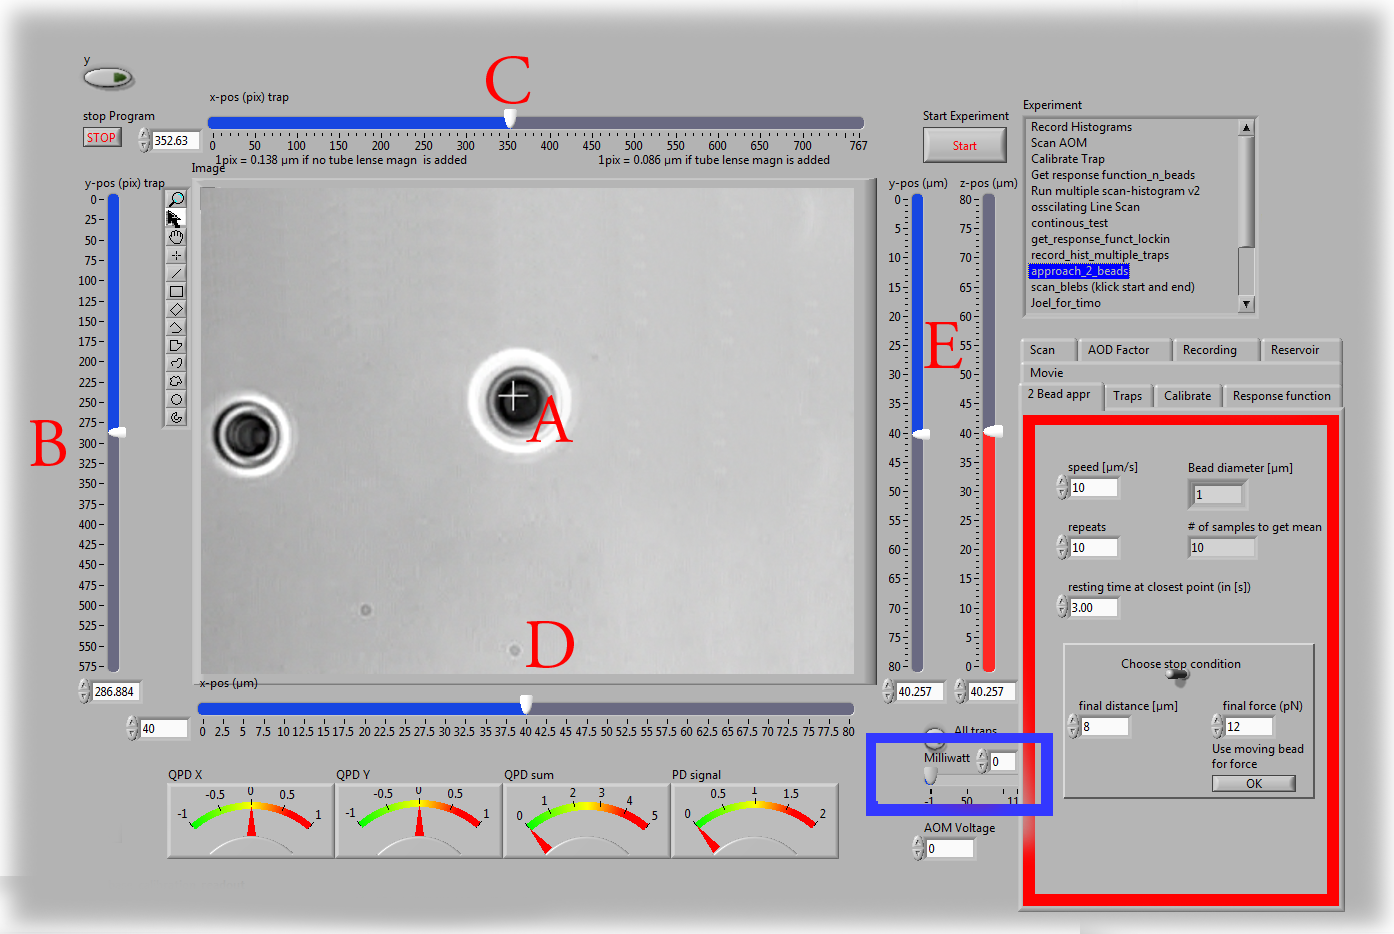
\includegraphics[width=0.900\linewidth]{frontend.png}
\caption{Software interface responsible for controlling the optical tweezer.  Sample
image showing 2 polystyrene beads and a single trap (A, white cross) holding one bead.
Cursors (B,C) are available to displace the optical trap(s).  Cursors can
control the position of the stage is X (D), Y (E, blue) and Z (E,red).
The blue rectangle highlights the slider that allows to control the trap power.  The red
rectangle highlights the area where the different parameters of the experiment
can be set (approach speed, resting time at closest point). 3 indicators at
the bottom of the screen indicate the voltage on the QPD.}\label{index-latex:fig-frontend}\end{figure}

The operator then captures one probe-bead and one actin-bead in each of the
traps.  Both types of beads can be recognized using fluorescent microscopy, as
actin-beads are promptly cover with a fluorescent actin
which  can clearly be distinguished from the probe bead that remains dark.
In the case where two identical beads are trapped one of the two traps can selectively
be disabled or decreased in stiffness, letting the bead escape from  the trap,
and the procedure can be repeated.

The operator will then move the two traps roughly one micrometer in each
direction to check that the two beads are effectively trapped in the tweezer and
that no external forces act on the beads.

For practical reasons, the traps are aligned along one of the principles axis
of the AOD before starting the indentation experiments.


\subsection{Indentations}
\label{index-latex:indentations}
The operator sets the parameters of the experiment in the software:
\begin{itemize}
\item {} 
Average bead radius,

\item {} 
Approach/Retraction Speed.

\item {} 
Resting Time

\item {} 
Laser Power

\end{itemize}

For each pair of actin/probe bead, the initial minimum approach distance of the
traps is set to 5 to 8 µm before a single indentation cycle is done. If the
maximum measured force between the two beads is not higher than 8 to 10 pN, the
minimum approach distance is reduced by 0.25 to 1 µm and the procedure
repeated. Once the maximum force measured is in the 10-15pN range the right
distance is found and up to 10 automatic force-indentation experiments are
performed (\hyperref[index-latex:bead-move]{Fig  \ref*{index-latex:bead-move}}) . Before each indentation the software automatically does a ``scan'' of
each bead to ensure correct calibration. An indentation cycle has the
following step:
\begin{itemize}
\item {} 
Probe trap is approaching the actin-bead at constant speed until the minimal approach distance has been reached.

\item {} 
At the minimal distance the traps remain stationary for the predefined (typical 3 seconds) resting time.

\item {} 
Probe trap returns to its initial position at constant speed.

\item {} 
Cycle is repeated as many times as set.

\end{itemize}

During this cycle the deflection of the laser induced by the probe-bead and
actin-bead are recored by the QPD.

After an indentation cycle is finished the experimenter can try to perform the
indentation on the actin-bead from another direction, or release the actin-bead
proceeding to a new one.

In the case where the indented actin network shows signs of inhomogeneity or
symmetry breaking, the experiments are stopped and not taken into account for
further analysis.

The date and time of each indentation cycle is recorded to extract the time of
polymerisation for each sample.
\begin{figure}[htbp]
\centering
\capstart

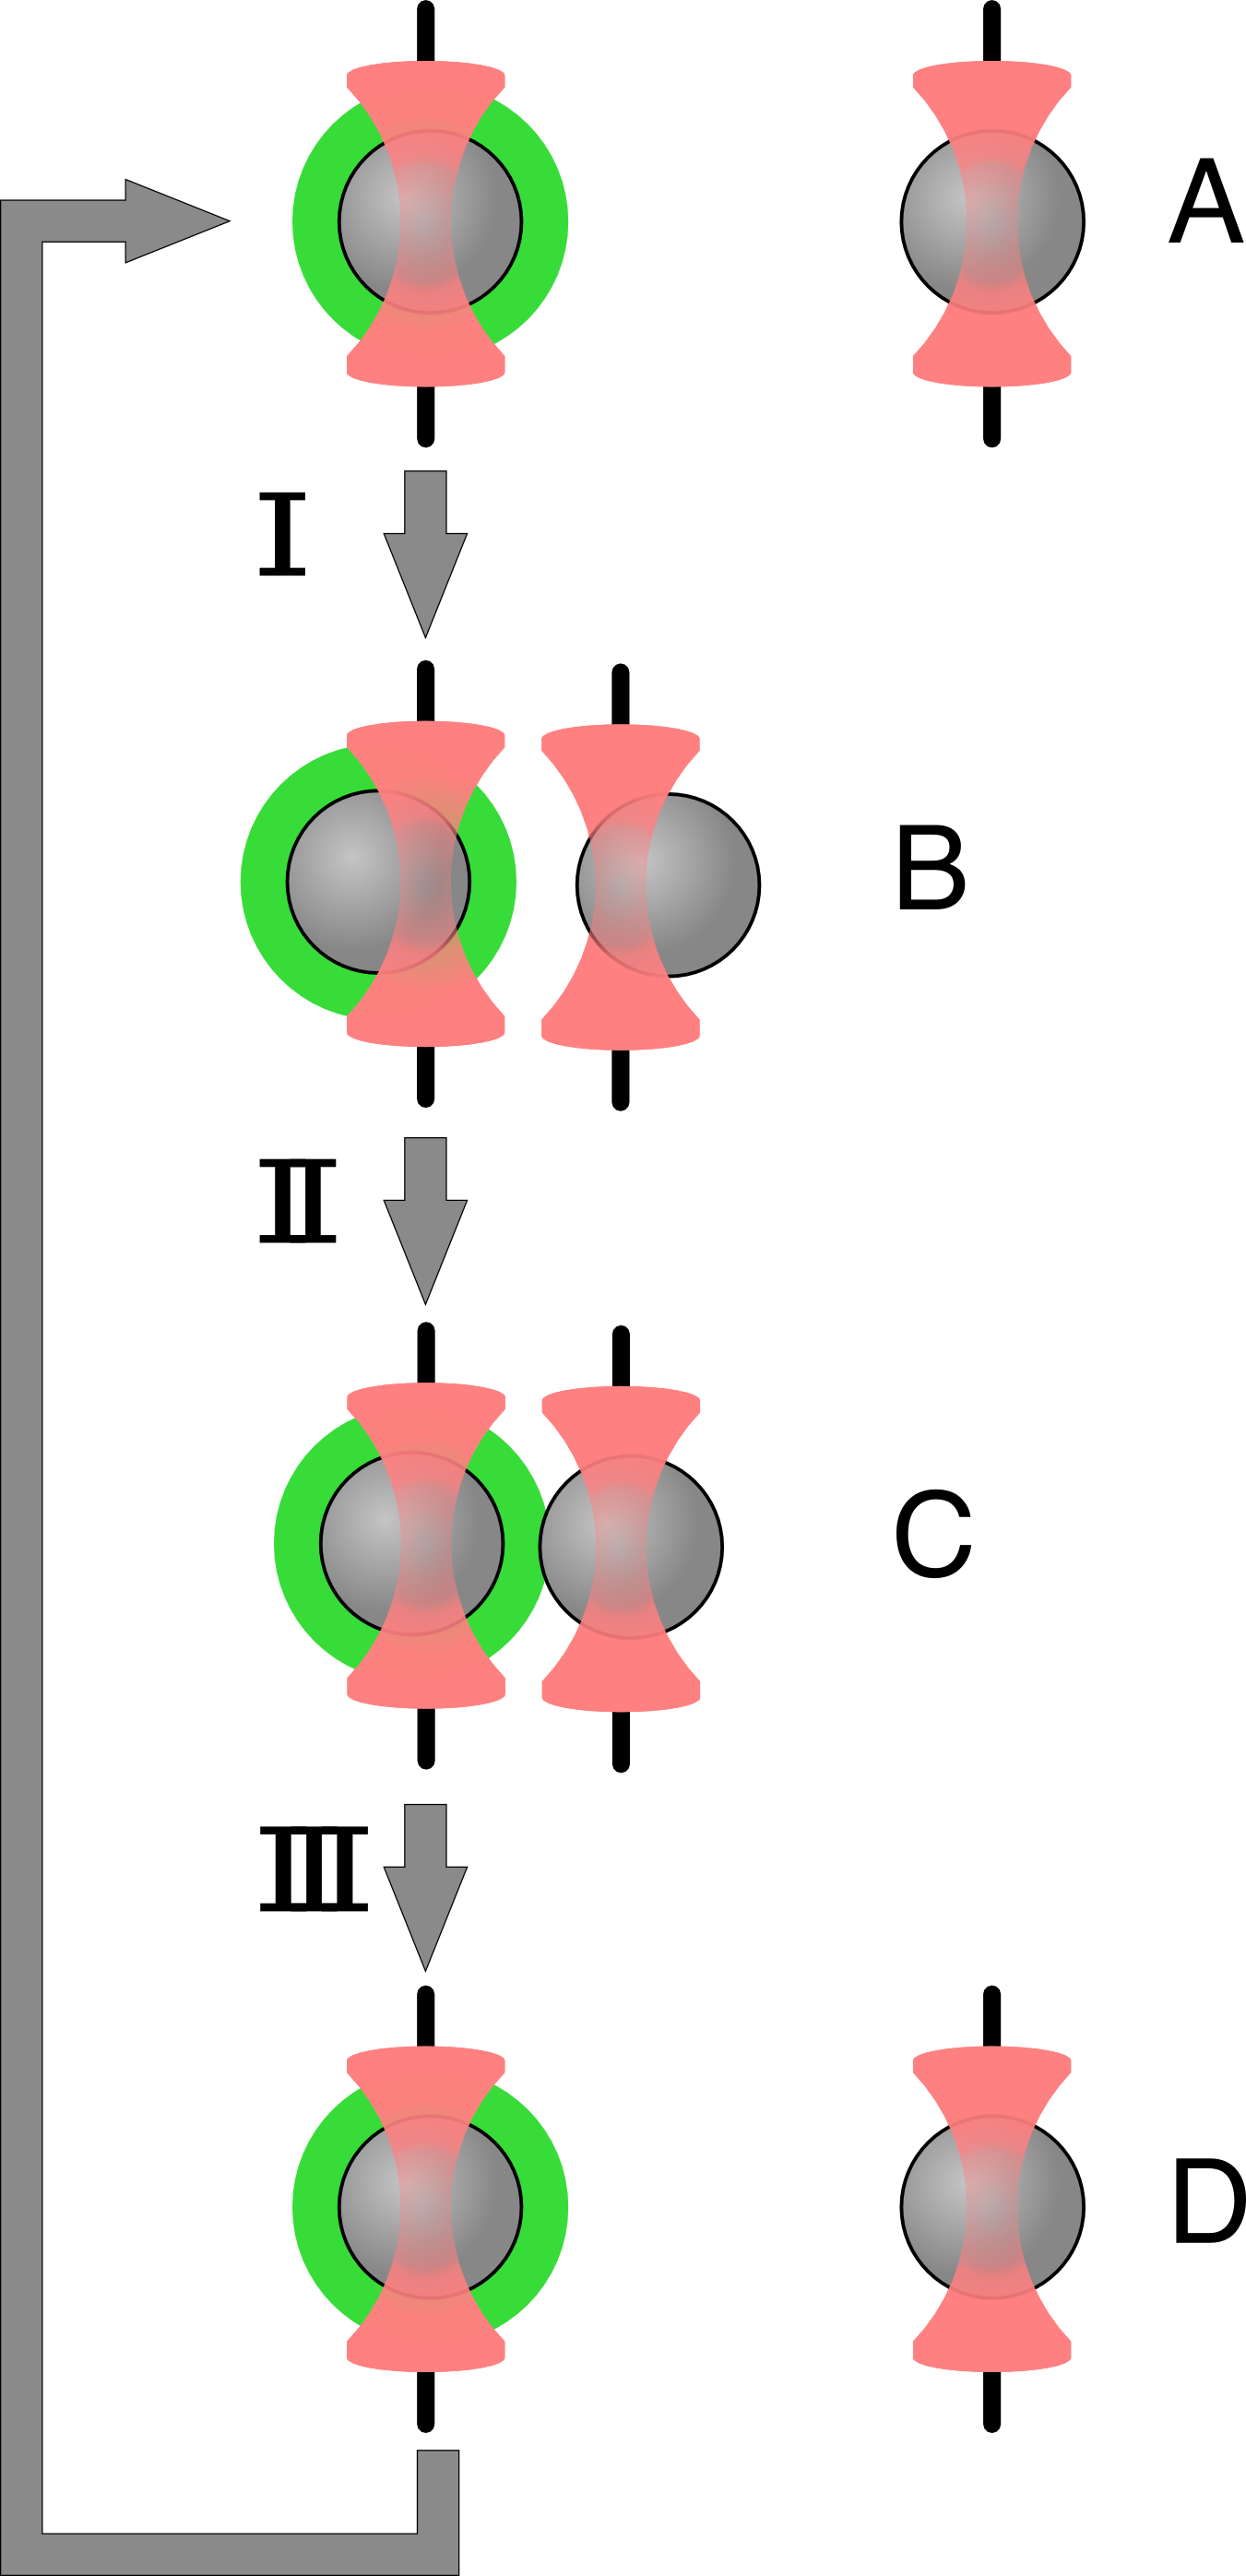
\includegraphics[width=0.500\linewidth]{beed_move.png}
\caption{Schematic of indentation experiment. On the left is the actin-bead, covered
with actin, in the static trap, on the right the probe-bead in the mobile
trap. At the beginning of the experiment (A) the probe bead is situated far from
the actin-bead. During the approach phase (I) the moving trap approaches
the static trap at 10µm/sec until it reaches the minimal approach
distance (B). The moving trap stays at the minimal approach distance for
3sec (II), which constitute the relaxation phase.C) The actin gel are
relaxed, the distance between bead is smaller than on B. III) the moving
trap retract at 10 µm/sec back to its initial position.}\label{index-latex:bead-move}\end{figure}


\section{Time Shared Optical Traps}
\label{index-latex:time-shared-optical-traps}\label{index-latex:time-shared-ot}
The optical trap is build on an inverted microscope (Olympus, IX71) equipped with
a fluorescence (200W mercury lamp, Osram, Munich, Germany). The sample is observed
through a Olympus 60X water immersion objective (Olympus) with numerical aperture NA=1.2, that also
serves at entry point for the laser of the optical tweezer.  The light source is
an infrared fiber laser (\(\lambda=1064nm\), YLP-1-1064, IPG,
Germany). X, Y positioning and stiffness of the trapping force are controlled
by 2 Acousto Optic Deflectors (AODs, AA-Optoelectronics, France) that are placed  in the conjugated plane of
the back focal plane of the objective.
Multiple traps can be achieved by switching the laser between
multiple positions within a switching time in the order of 5 µs, and resting
on each position 20µs or more.

Light refracted by the trapped sample is collected by a 40X (N.A:0.9, Olympus)
water immersion objective and imaged on a quadrant photodiode (QPD) conjugated
with the back focal plane of the light collection objective. Signals from the
QPD (\(\Delta X, \Delta Y\) and \(\Sigma\)) are sampled at 500kHz, by a Digital
To Analogic Aquisition card (NI PCIe-6363, National Instruments, Austin,
Texas), controlled using a custom written Labview software (National Instruments)
coupled with Matlab (Mathworks, Natick, MA). Raw signals are preprocessed by binning all
voltage measured during the time the laser rest (typically 20µs) at one position. Finally
the mean and standard deviation for each trap visit is stored for further processing.

The trap stiffness is inferred from bead radius, laser power, number of present
traps and control experiment data. In control experiments the trap stiffness is
calibrated using the power spectral density method, and was determined
to be as high as 80 pN/µm at full laser power (119mW) for a single trap.
In the case of multiplexing two traps as used in this work, both traps were calibrated before
the experiment.
Coarse positioning of the sample is done through a pair of micrometer precision
screws capable of translating the microscope stage in X and Y.  Finer
positioning in X,Y and Z direction are done with the help of a 3D piezo stage with an
accessible range of 80 µm in each direction and a sub-micrometer accuracy.


\section{Oocyte}
\label{index-latex:oocyte}

\subsection{Oocyte obtention}
\label{index-latex:oocyte-obtention}
Oocyte culture, collection and micro injection where done at College de France by Maria Almonacid.

Oocytes were collected from 11 to 15 week old mice (WT), fmn2-/- as previously
described in {\hyperref[index-latex:holubcova2013]{{[}Holubcova, Howard, Schuh,  2013{]}}} and maintained in Prophase I in M2+BSA
supplemented with  1µM Milrinone. Oocyte are then injected with cRNA  using a
micro-injector Eppendorf FemtoJet. Imaging was carried out at \(37^\circ{}C\).


\chapter{Mechanical properties of a far reaching actin cloud}
\label{index-latex::doc}\label{index-latex:mechanical-properties-of-a-far-reaching-actin-cloud}

\section{Introduction}
\label{index-latex:introduction}
We have seen that the actin cytoskeleton plays a major role in
cellular mechanics. It is necessary for force generation, and a
key component for cell motility. It has also be extensively studied both in
cells and biomimetic systems.

Actin can form a variety of networks in cells, ranging from dense branched
networks at the leading edge of the lamellipodia to bundled parallel structures
forming the filopodia.  Reconstruction of the actin network has been achieved in
biomimetic systems using purified components {\hyperref[index-latex:plastino2005]{{[}Plastino, Sykes,  2005{]}}},
{\hyperref[index-latex:loisel1999]{{[}Loisel, Boujemaa, Pantaloni, Carlier,  1999{]}}}, {\hyperref[index-latex:bernheim-groswasser2002]{{[}BernheimGroswasser, Wiesner, Golsteyn,  et al.  2002{]}}},  {\hyperref[index-latex:pontani2009]{{[}Pontani, vdGucht, Salbreux,  et al.  2009{]}}}, and
many properties of these network have been measured.

It has been determined that the actin cortex provides mechanical support for the
plasma membrane and that it extends over a few hundreds of nanometers. Many
cellular processes hint for actin structures connected to this cortex to be
key elements in organelle and chromosome positioning.

In this part of the manuscript we investigate how a sparse actin structure can
emanate from the actin cortex, and we explore its properties. Using the
{\hyperref[index-latex:bead-motility-assay]{\emph{bead-motility}}} (\autopageref*{index-latex:bead-motility-assay}) biomimetic system to reconstitute
the actin cortex and its dendritic structure, we show that a sparse network of
actin filaments emanating from the cortex has a mechanical effect sufficient to
displace objects on the size of cells organelles at distances up to tens of micrometers
away from the actin cortex.

The branched structure of the actin cortex underneath the plasma membrane of
cells hints for a structure governed by Arp2/3. How Arp2/3 and CP can be used
to form a biomimetic actin cortex has been widely studied. In
{\hyperref[index-latex:kawska2012]{{[}Kawska, Carvalho, Manzi,  et al.  2012{]}}}, both \emph{in vitro} measurements on reconstituted actin cortices
on beads as well as simulations investigate the effect of cross-linking and
Capping Protein on the formed actin gel. It can be seen both experimentally and in
simulation that a network of filaments escape from what is defined as the actin
cortex (\hyperref[index-latex:fig-bead-tirf]{Fig  \ref*{index-latex:fig-bead-tirf}}). The effect of these long filaments is not taken into account in the
\emph{in-silico} system where the analysis is restricted to filaments shorter than 10
µm. Only the effect of dense entangled actin networks generated from primers
randomly placed  on the bead surface participate in the increase of tension and
contribute to symmetry breaking.
\begin{figure}[htbp]
\centering
\capstart

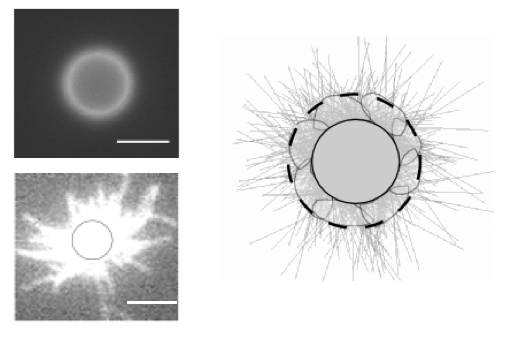
\includegraphics[width=0.700\linewidth]{Bead-tirf-fluo-sim.png}
\caption{Upper Left : Fluorescence image of an actin bead with a growing actin
cortex. Escaping filaments form the actin cloud that can only hardly  be
seen in fluorescence. Scale bar is 2 µm. Lower Left: Total Internal Reflexion (TIRF) image
of actin polymerising on an actin bead. Escaping filaments are directly
visible. The gray circle represents the size of the bead.  Right :
Representation of the actin growth simulation with delimitation between the
entangled branched actin network and escaping filaments.  Adapted from
{\hyperref[index-latex:kawska2012]{{[}Kawska, Carvalho, Manzi,  et al.  2012{]}}}.}\label{index-latex:fig-bead-tirf}\end{figure}

The limit of the dense network visible in epifluorescence is defined in
{\hyperref[index-latex:kawska2012]{{[}Kawska, Carvalho, Manzi,  et al.  2012{]}}} by the position of the half-maximum fluorescent intensity (\hyperref[index-latex:fig-intensity-profile]{Fig  \ref*{index-latex:fig-intensity-profile}}).
The properties of these networks are measured by {\hyperref[index-latex:pujol2012]{{[}Pujol, dRoure, Fermigier, Heuvingh,  2012{]}}} using
magnetic beads and actin stabilized with phalloidin. Though they do not
investigate the sparse and softer actin network that originate from the visible
part.

Using {\hyperref[index-latex:time-shared-ot]{\emph{time-shared optical tweezer}}} (\autopageref*{index-latex:time-shared-ot}) we are able to probe
the mechanics of this soft actin structure at time scale shorter than the
characteristic time of actin polymerisation and forces in the pN range. We show
that beyond the dense dendritic network mimicking the actin cortex which as
been measured to have an {\hyperref[index-latex:elastic-modulus]{\emph{elastic modulus}}} (\autopageref*{index-latex:elastic-modulus}) in the order of
kPa {\hyperref[index-latex:pujol2012]{{[}Pujol, dRoure, Fermigier, Heuvingh,  2012{]}}} the soft actin cloud is much softer with
a stiffness in the Pa regime.  This might explain why such a
structure has not previously been seen by less sensitive techniques than optical
tweezers. The size of this actin cloud and its ability to sustain forces
suggest that in cells the actin cortex is not sharply delimited and that
structures escaping from it may have a role in organelle positioning.

The questions we address in this part of the manuscript are :  How does the far
extends the soft part of the gel? What are its precise mechanical properties?  How does it change
over time?  Is the actin cloud elastic or viscous?
\begin{figure}[htbp]
\centering
\capstart

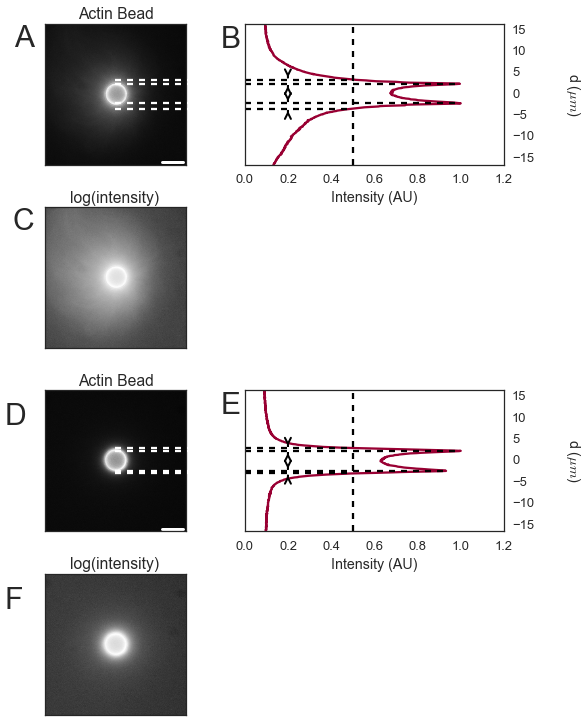
\includegraphics[width=0.800\linewidth]{intensity_profile_xnM_Arp_xnM_CP_xmin.png}
\caption{A) Epifluorescence image of polystyrene bead with a growing actin gel in
presence of 25 nM of Arp2/3 and 25 nM of Capping Protein. Scale bar is 5
µm.  B) Normalized intensity profile of fluorescence image with thickness
of the gel shown with dashed line as defined in {\hyperref[index-latex:kawska2012]{{[}Kawska, Carvalho, Manzi,  et al.  2012{]}}} :
Distance between maximum intensity and half-maximum intensity.  C)
Epifluorescence image of log(intensity). D,E,F) Same as A,B,C, in absence
of Capping Protein}\label{index-latex:fig-intensity-profile}\end{figure}


\section{Actin-Bead System}
\label{index-latex:actin-bead-system}
To reproduce the actin cortex and study the mechanics of actin structures
emanating from it {\hyperref[index-latex:bead-preparation]{\emph{we prepare polystyrene beads}}} (\autopageref*{index-latex:bead-preparation}) of 4.3
µm diameter coated with a nucleation promoting factor. Theses beads are placed
in the {\hyperref[index-latex:atp-mix-buffer]{\emph{ATP mix buffer}}} (\autopageref*{index-latex:atp-mix-buffer}) in presence of 25nm of Arp2/3
complex, 4µm of monomeric actin (20\% fluorescently labeled) 12 µM profilin and
a variable amount of Capping Protein. {\hyperref[index-latex:m-et-m]{\emph{see Material and Methods}}} (\autopageref*{index-latex:m-et-m}).
These beads are referred to as actin-beads.

These condition are chosen in order to grow a dense network on the surface of
actin-bead as in {\hyperref[index-latex:kawska2012]{{[}Kawska, Carvalho, Manzi,  et al.  2012{]}}}. We place ourself at 25nM ATP and a varying
amount of Capping Protein concentration in order to cover condition where the
dense gel that forms on the actin-bead is able to accumulate sufficient stress
to lead to symmetry breaking (CP between 15  and 35 nM, see part {\hyperref[index-latex:bead-motility-assay]{\emph{Bead Motility Assay}}} (\autopageref*{index-latex:bead-motility-assay})). We also investigate
conditions where the amount of Capping Protein is too low (\textless{} 15nM) or too high
(\textgreater{}35 nM) to permit symmetry breaking.

We select a bead diameter of 4.3 µm in order to get a characteristic symmetry
breaking time of 20 to 40 minutes.
A smaller bead radius imply a
faster increase of stress and a shorter symmetry breaking time.
The choice of 4.3µm provides sufficient time to proceed with the
experiments before symmetry breaking occurs.

All measurements were made on an actively growing actin network which
was not stabilized and before symmetry breaking
occur for Capping Protein concentration in the range 15 to 35 nM {\hyperref[index-latex:kawska2012]{{[}Kawska, Carvalho, Manzi,  et al.  2012{]}}}.


\section{Probe Bead System}
\label{index-latex:probe-bead-system}
Beside the actin-bead, the experiment requires a polystyrene bead passivated
with BSA. These beads are referred to as probe-beads.  The size of the
probe-bead was chosen to be the same as the actin-bead, which ensure optical
trapping of both beads in the same observation plane. In the case of beads with
different diameters, the axial forces on the beads are different. This axial
displacement of the two beads during the indentation process leads to a
component along the z-axis which  eventually pushes one bead out of the trap.


\section{Experimental description}
\label{index-latex:experimental-description}
To probe the actin network we trap an actin-bead with a growing actin-network
and a probe-bead using time-shared {\hyperref[index-latex:time-shared-ot]{\emph{optical trap}}} (\autopageref*{index-latex:time-shared-ot}),  and
measure the forces on the actin-bead using a QPD placed in the back focal plane of
the condenser ({\hyperref[index-latex:m-et-m]{\emph{material and methods}}} (\autopageref*{index-latex:m-et-m})).

To avoid systematic errors of force measurements on the moving trap, all force
recordings used for analysis are made on the static bead, which is in our case the actin bead.

The indentation is a three step process (\hyperref[index-latex:figindent-time]{Fig  \ref*{index-latex:figindent-time}}):
\begin{itemize}
\item {} 
Approach phase at constant velocity 10µm/sec unless specified otherwise

\item {} 
Relaxation phase of 3 second during which both traps remain static

\item {} 
Retraction phase in which the probe trap move towards its initial position at 10µm/sec.

\end{itemize}


\subsection{Approach Phase}
\label{index-latex:approach-phase}
During the approach phase, the probe-trap approaches the actin-trap at constant speed (10 µm/s), as shown in
\hyperref[index-latex:figindent-time]{figure  \ref*{index-latex:figindent-time}} for times \(t < t_1\). During this approach the actin bead
will repel the probe bead due to the actin network growing on it. The force felt
by the actin bead will progressively increase during the probe bead approach,
eventually reaching the maximum as the probe-trap reaches its closest position
to the actin trap. Note that during this process
the force between the beads pushes  the beads out of the respective trap center.
The displacement of the beads in the trap remains small compared to the
distance between the two beads. Hence in the following we consider that the probe-bead speed is equivalent to the trap approach speed of 10µm/sec.


\subsection{Relaxation Phase}
\label{index-latex:relaxation-phase}
After the approach , the trap remain static for a 3 seconds relaxation phase
. The relaxation phase start at \(t_1\) and
finish at \(t_3\) as shown on \hyperref[index-latex:figindent-time]{figure  \ref*{index-latex:figindent-time}}. The duration of the relaxation phase is sufficient to allow the partial
relaxation of the actin cloud  but remain sufficiently short compared to
the actin polymerisation speed hence the polymerisation is not expected to
change the properties of the network during indentation cycle as well as
during repetitive indentation (\hyperref[index-latex:reproc]{Figure  \ref*{index-latex:reproc}})

While the actin network relaxes, the forces between the two beads will slowly
decrease thus leading to the beads getting closer to their trap center and
closer to each other. The decrease in distance during the relaxation phase is
small compared to the distance between beads. The decrease of force as well as
the minimal change in distance between the two bead can be seen on \hyperref[index-latex:figindent-time]{Fig  \ref*{index-latex:figindent-time}}
in the middle part.
\begin{figure}[htbp]
\centering
\capstart

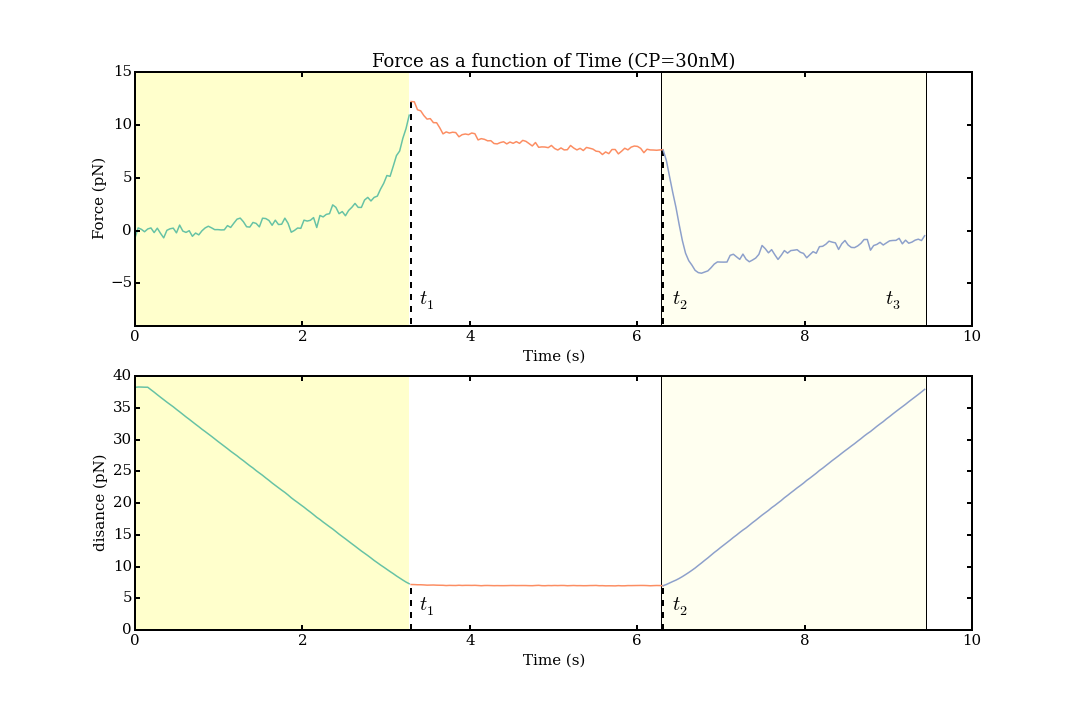
\includegraphics[width=0.700\linewidth]{force_time.png}
\caption{Upper graph : Force as a function of time on the actin-beads.  Lower graph
: distance between beads (distance between traps + displacement of beads
from the trap center) as a function of time. First part of each graph
(green curve, yellow back) represents the approach phase. Middle part
(orange on white) corresponds to the relaxation phase, and right part (blue on pale
yellow) is the retraction.  Shown data is a subsample of around 1 of every
1000 points acquired. We can see on the second graph that the bead
displacement on their respective trap is small compared to the
displacement of the trap and justify the approximation of a probe bead
speed equal to the probe trap speed.}\label{index-latex:figindent-time}\end{figure}


\subsection{Retraction part}
\label{index-latex:retraction-part}
After the three seconds of the retraction phase, the probe trap returns to it's
initial position at 10 µm/s (\(t > t_2\)). During this phase, the force
exerted between the two beads decreases, becomes negative, reaches a minimum, and
eventually returns to zero as the probe bead recover its initial
position (shown on \hyperref[index-latex:figindent-time]{Figure  \ref*{index-latex:figindent-time}} right part). Negative forces
represent forces that tends to push the two beads towards each other.


\subsection{Reconstitution of Force-distance-curve}
\label{index-latex:reconstitution-of-force-distance-curve}
From the position of he trap with time and the signal measured by the QPD the
position of bead in the trap as well as the force exerted on each bead can be
calculated. We can then recover the distance between bead centers as a function
of time.  The force-distance curve representing the force exerted by the
probe bead on the actin bead as a function of the distance can be computed and is
show in \hyperref[index-latex:force-distance]{figure  \ref*{index-latex:force-distance}} where we can still distinguish the three
phase of the indentation cycle, also marked by the color of the data.
\begin{figure}[htbp]
\centering
\capstart

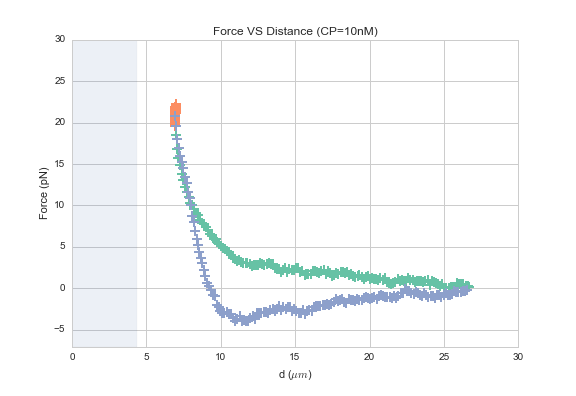
\includegraphics[width=0.800\linewidth]{force-distance.png}
\caption{Force exerted on the actin bead as a function of the distance between the
two bead centers. Color and data are the same as in \hyperref[index-latex:figindent-time]{Fig  \ref*{index-latex:figindent-time}}.
The probe bead starts from the far right, and gets closer
while the force increases (green upper part of the curve), reaches a
maximum, and enters the relaxation phase (orange part) where the force
between the probe and actin bead decrease, while the distance  also
slightly decreases. During the retraction part (blue) the force rapidly
decreases and  reaches negative values while the bead returns to its initial
position. Shown data is a subsample of 1 every 1000 points of acquired
data. Shaded region represent areas where the two polystyrene beads would
interpenetrates.}\label{index-latex:force-distance}\end{figure}


\subsection{Repetitive indent}
\label{index-latex:repetitive-indent}
To check for reproducibility and non-plastic deformation of the network after
indentation, the indentation cycle can be repeated several times at a few seconds
interval. As the network is constantly growing during the measurement, this
repeat also allows to check for possible change of network properties due to actin
polymerisation. The force distance plot is shown in \hyperref[index-latex:reproc]{Figure  \ref*{index-latex:reproc}} \hyperref[index-latex:reproc-time]{,  \ref*{index-latex:reproc-time}}.
\begin{figure}[htbp]
\centering
\capstart

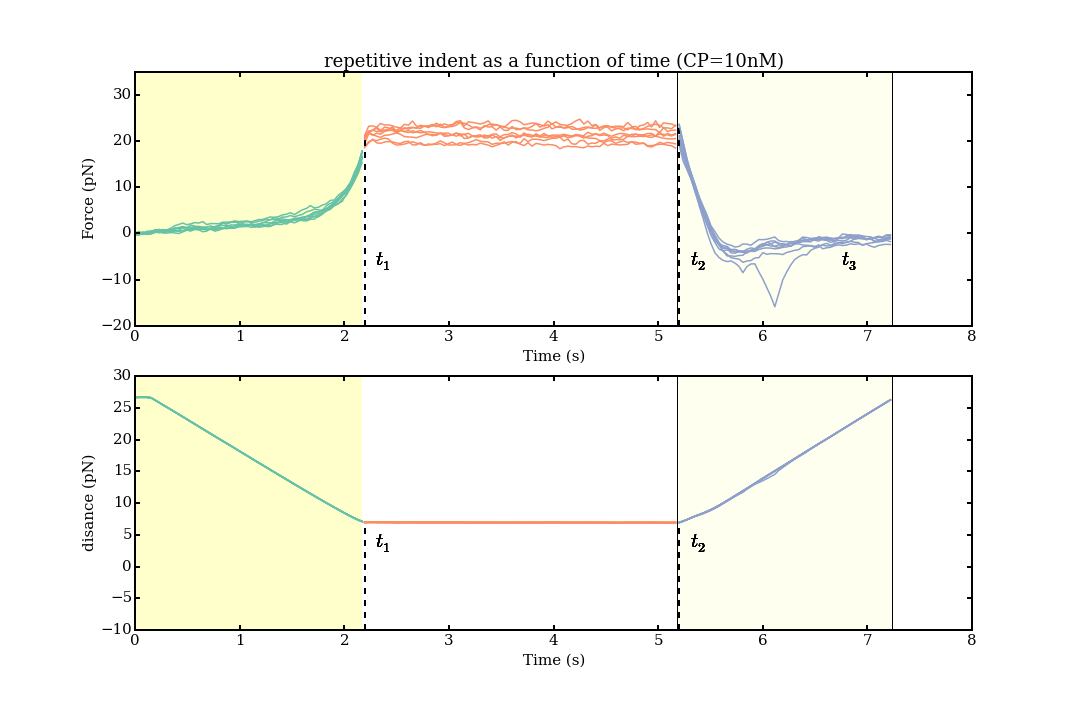
\includegraphics[width=1.000\linewidth]{reproc-time.png}
\caption{Upper graph : Force exerted on actin bead as a function of time for ten
repetitive indents. In one of the cycles a sticking event can be seen in the
retraction phase 6 seconds after the beginning of the cycle. Lower graph:
Distance as a function of time for  ten repetitive indents. The ten curves
can only hardly be distinguished from one another, which shows the
reproducibility of indentation curves.}\label{index-latex:reproc-time}\end{figure}
\begin{figure}[htbp]
\centering
\capstart

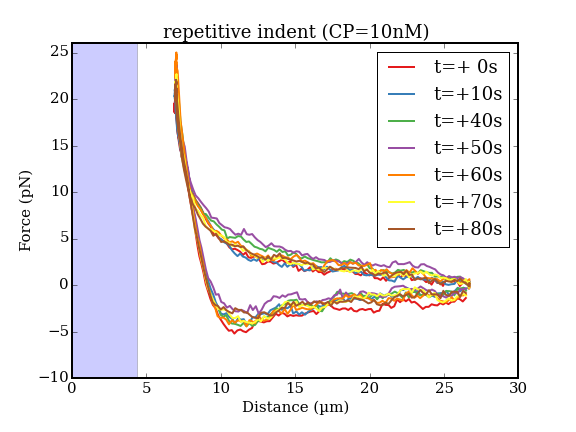
\includegraphics[width=0.800\linewidth]{reproc.png}
\caption{Figure showing the reproducibility of indentation process on a bead with
25nM Arp2/3 and 10nM CP Subset of data from \hyperref[index-latex:reproc-time]{Fig  \ref*{index-latex:reproc-time}} shown
with different color to represent the evolution of the indentation curve
over time.  Time is relative to first indentation. Shaded area represent
zone where the two beads would interpenetrates.}\label{index-latex:reproc}\end{figure}


\subsection{Effect of approach speed}
\label{index-latex:effect-of-approach-speed}
{\hyperref[index-latex:gardel2003]{{[}Gardel, Valentine, Crocker,  et al.  2003{]}}} suggest that for frequencies higher than 0.1 Hz, force due to
the viscous behavior  of actin network can be in the same order as the elastic
component. To test if such an relaxation effect is important we measured the effect of the
approach speed on the force measurements. \hyperref[index-latex:many-speed]{Fig  \ref*{index-latex:many-speed}} presents the
indentation speed affect the measurement by varying the approach speed from 10
to 30 µm/s on the same actin bead.
\begin{figure}[htbp]
\centering
\capstart

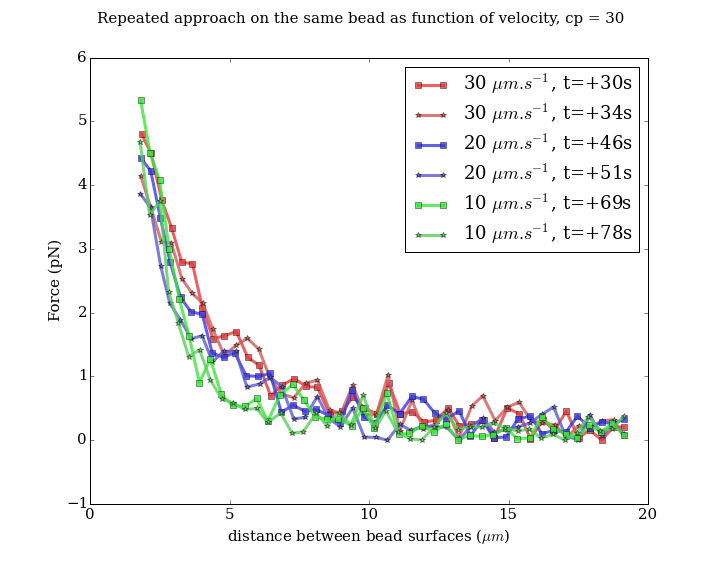
\includegraphics[width=0.600\linewidth]{many_speed.png}
\caption{Approach phase of repetitive indents at multiple speed on the same
actin-bead. The approach phase in the different conditions are similar,
hinting for a negligible effect of the viscosity  in the actin cloud at the
speed considered.}\label{index-latex:many-speed}\end{figure}


\section{Experimental observations}
\label{index-latex:experimental-observations}
Using the bead system, we are able to reconstruct actin cortices \emph{in vitro} and
to investigate the mechanical properties inaccessible to other microscopy
techniques like TIRF. Beyond the visible actin cortex we can detect the
presence of an actin structure that has mechanical effects starting at
distances of \(> 10\mu{}m\), hence far beyond the thickness of the actin cortex (\textasciitilde{}1µm).
\hyperref[index-latex:cloud-repelling]{Figure  \ref*{index-latex:cloud-repelling}} presents a video showing qualitatively that the actin cloud growing
on actin beads is able to repel free floating probe beads before they reach the
visible reconstituted cortex.

To quantify the distance at which the probe beads are first affected by the actin-cloud
we measure the experimental noise by looking at the fluctuations of the trapped probe bead.

During the indentation we defined \(d_0\) as the distance at which the
average force felt by the probe bead is higher than the experimental noise.
Typically the standard deviation is 2pN.

The repartition of \(d_0\) with the concentration of Capping Protein is
plotted in \hyperref[index-latex:d0-violin]{figure  \ref*{index-latex:d0-violin}}.
\begin{figure}[htbp]
\centering
\capstart

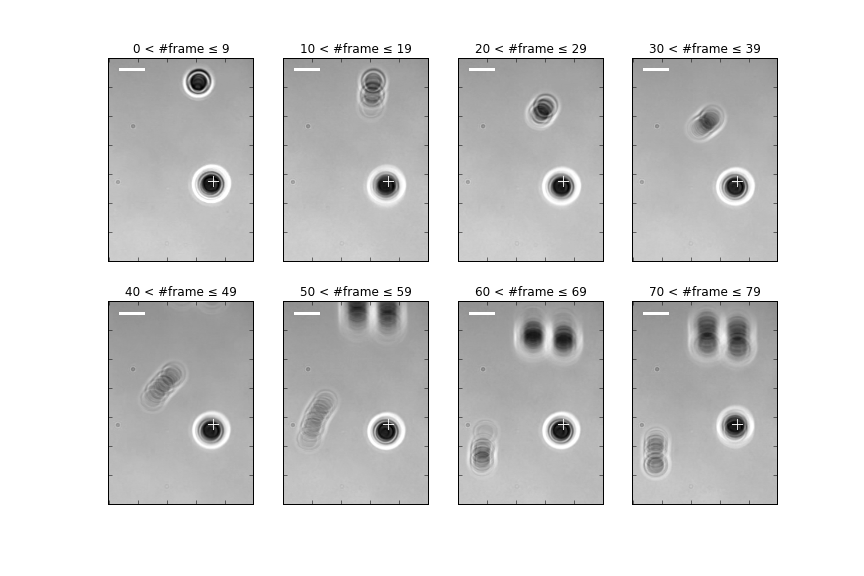
\includegraphics[width=0.850\linewidth]{cloud-repelling.png}
\caption{Chronophotography representing the displacement a trapped actin bead in a
solution with probe bead. During this experiment, the actin bead is kept
static in the optical trap (marked by the cross) while the stage is moved.
Scale bar is 5 micrometers. Total movie duration is 21 seconds.}\label{index-latex:cloud-repelling}\end{figure}
\begin{figure}[htbp]
\centering
\capstart

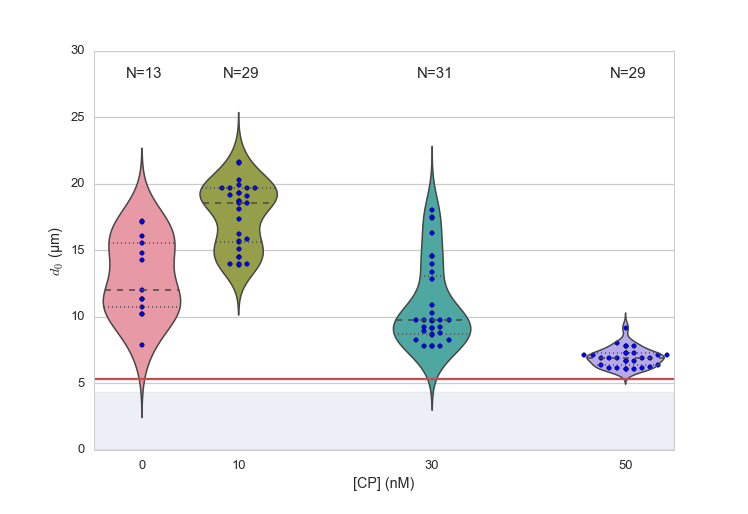
\includegraphics[width=0.650\linewidth]{d0_violin.png}
\caption{Repartition of the bead-center distance at which the actin cloud exert a
force higher than the noise (\(d_0\)) on the probe bead, as a function of
Capping Protein. Shaded region represent the position of the bead surface
(4.34 µm) and the red line represent the bead surface+1µm (upper bound for
the in vitro
Capping Protein concentration. The shaded region represents the position of
the bead surface (4.34 µm) and the red line represents the bead surface+1µm
(upper bound for the in vitro
reformed actin cortex measured in {\hyperref[index-latex:kawska2012]{{[}Kawska, Carvalho, Manzi,  et al.  2012{]}}}). We see in this graph that for symmetry breaking
conditions (CP 10 nM and 30 nM) the distance at which the actin cloud starts to apply
forces on the probe bead is large compare to the thickness of the actin
cortex. The distance at which the probe bead is able to detect the presence
of the actin cloud decreases when increasing the concentration of Capping
Protein that restricts  actin filament growth. The condition in the absence
of Capping Protein are a particular case as no dense actin network forms
on the surface of the actin bead.}\label{index-latex:d0-violin}\end{figure}


\subsection{Approach phase modeling}
\label{index-latex:approach-phase-modeling}
To extract mechanical properties using the three phases of the experiment we
decided to model each part (approach, relaxation and retraction) independently.
In particular, we fit force-distance curve of the approach phase using a power
law with 3 fit parameters \(\alpha, \beta, \delta\):
\phantomsection\label{index-latex:equation-eqa31}\begin{gather}
\begin{split}F(d) = \beta \times \left(d-\delta\right)^\alpha\end{split}\label{index-latex-eqa31}
\end{gather}
In which \(F\) represent the force exerted on the probe bead, and \(d\)
is the distance between bead centers. The powerlaw exponent \(\alpha\) is
expected to be negative as the force decreases with the distance \(d\), and
characterizes how fast the force increase as the two
beads approaches each other. The prefactor \(\beta\) acts as a scaling factor of the
force. The offset parameter \(\delta\) shifts the curve on the distance
axis. This phenomenological model has the particularity that the force on the probe bead tends to
\(+\infty\) when the distance \(d\) get  to \(\delta\). The force
is undefined for values of \(d< \delta\). Hence, the offset distance \(\delta\)
practically describe the distance at which the optical trap is not able to
indent the network anymore.

In the case of a hard sphere the value of \(\alpha\) would tend towards
\(-\infty\) leading to a infinite force increase at the contact between the
two hard-spheres of same diameter and a value of \(\delta\) equal to the
diameter of the hard sphere.  In this case \(F(d>\delta)=0\) and
\(F(d<\delta)=\infty\)

The optical tweezer we use can apply forces up to 20pN, and the beads we use
have a diameter of 4.34µm , hence we determine a cross-sectional surface of surface of roughly \(14.7\mu{}m^2\). Before
escaping the trap, the probe bead can move up to 1µm from its
trap center. To estimate the maximal stiffness that can be measured, we approximate that we can
provide a clear measure of deformation in the order of 1/10 of µm,  this
leads to a maximum detectable Young's modulus of :
\phantomsection\label{index-latex:equation-eqa32a}\begin{gather}
\begin{split}E_{max} &\sim \frac{F_{max}L_{0,max}}{A_0.\Delta L} \\
        &\sim \frac{50.10^{-12} \times 1.10^{-5} }{  (\pi\times 2.17\times 10^{-6})^2 \times 1.10^{-7}              }\\
        & \sim 300 Pa\end{split}\label{index-latex-eqa32a}
\end{gather}
Any material with a stiffness much higher than 300 Pa can be considered as
infinitely rigid.

The elasticity of dense actin gels around polystyrene beads has been measured
in {\hyperref[index-latex:pujol2012]{{[}Pujol, dRoure, Fermigier, Heuvingh,  2012{]}}} and found to be in the order of kPa.  Therefore the
optical tweezers are not able to probe the mechanics of the dense gel on the
surface of the bead. The value of \(\delta\)  is expected to be \(> 4.34 \mu{}m\) as it include partially the dense actin gel.

The model can be fitted independently on each experimental
approach phase. An example of such a fit is shown in
\hyperref[index-latex:force-distance-fit]{figure  \ref*{index-latex:force-distance-fit}} and the quality of fit can be measure by the
coefficient \(R^2\) which has a media value of \emph{0.97}
across all fits.
\begin{figure}[htbp]
\centering
\capstart

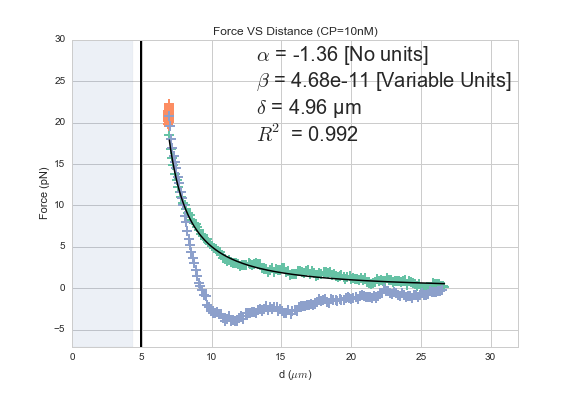
\includegraphics[width=1.000\linewidth]{force-distance-fit.png}
\caption{Power law model fitted on the approach phase data for one experiment in the
presence of {[}CP{]}=10nM, with the particular values found for the fit
parameters.  The vertical line represent the point at which the model
diverges and the force goes to infinity, that is to say \(\delta\). The
shaded region corresponds to the distance at which the two beads would
interpenetrates. Relaxation (orange) and retraction (blue) data are not fitted.}\label{index-latex:force-distance-fit}\end{figure}

The approach phase data can be corrected for the distance offset \(\delta\)
and plot in a log-log scale allowing for a better appreciation of the fit
result (\hyperref[index-latex:force-distance-log-log]{Fig  \ref*{index-latex:force-distance-log-log}}). The corrected distance is noted with  \emph{c} indices \(d_c = d-
\delta\). In the model the force tends to infinity at \(d_c = 0\).
\begin{figure}[htbp]
\centering
\capstart

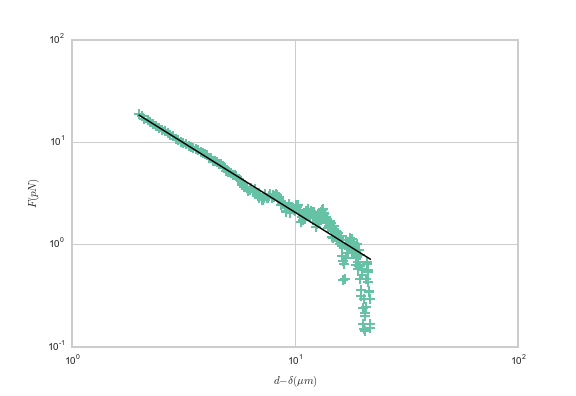
\includegraphics[width=0.800\linewidth]{force-distance-fit-loglog.png}
\caption{Force on the actin bead  during the approach phase as a function of bead distance
minus distance offset \(\delta\) plotted on a log-log scale. Black line
represents the power law model with  correction of the offset distance. Same
data as \hyperref[index-latex:force-distance]{Fig  \ref*{index-latex:force-distance}} but showing only approach phase.}\label{index-latex:force-distance-log-log}\end{figure}

In our experiments, the polystyrene beads have an average diameter of 4.34 µm,
thus we expect \(\delta\) to be higher than the bead diameter since the beads cannot interpenetrates.  Data with
\(\delta\) values lower than 4.34 µm (21 out of 127) are considered as
unphysical and were removed from further analysis.

As expected we find negative values for \(\alpha\). Surprisingly the value
of alpha does not vary significantly when comparing experiments with different
amount of Capping Protein and stay close to -1, with a mean value of -1.10, and
a standard deviation of 0.38. The distribution of the power law exponent can be
seen on \hyperref[index-latex:power-law-exponent]{figure  \ref*{index-latex:power-law-exponent}}
\begin{figure}[htbp]
\centering
\capstart

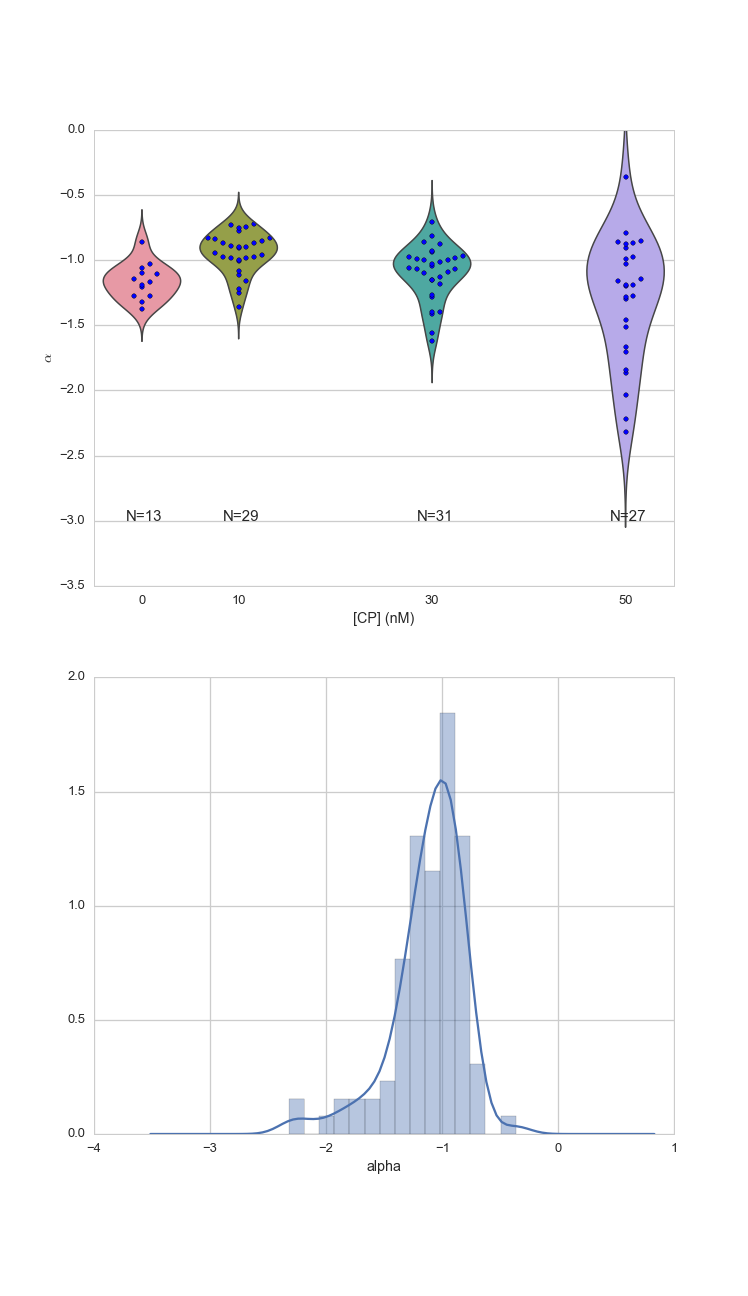
\includegraphics[width=0.600\linewidth]{alpha_violin.png}
\caption{Right : Violin plot showing the repartition of power law exponents with the
concentration of Capping Protein. Left: distribution of power law exponent
\(\alpha\) regardless of the concentration in Capping Protein. Value of
exponent lies close to \emph{-1}.}\label{index-latex:power-law-exponent}\end{figure}

Due to the scale invariance of the inverse power law found above,  all the
approach phases data can be rescaled into a single master-curve (\hyperref[index-latex:fig-rescale-powerlaw]{Fig  \ref*{index-latex:fig-rescale-powerlaw}}). This is done
by dividing the force by the maximum force \(F_{max}\) reached during the
approach and rescaling the distance by the minimum approach distance from which
\(\delta\) is subtracted.
\begin{figure}[htbp]
\centering
\capstart

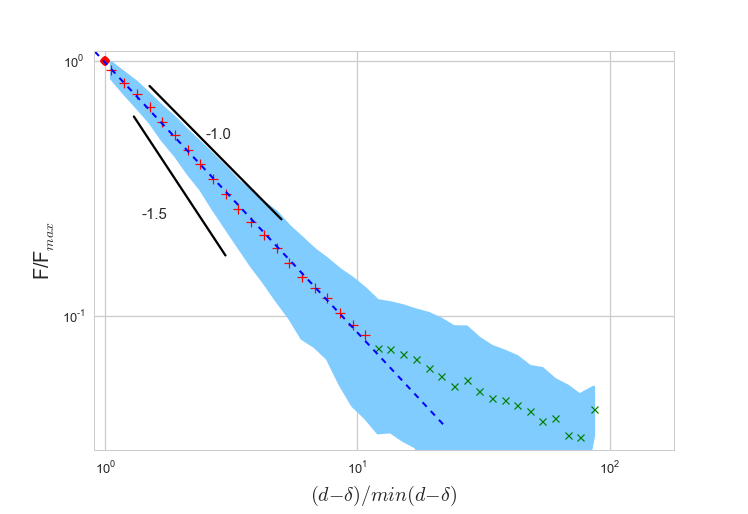
\includegraphics[width=0.700\linewidth]{rescaled_powerlaw.png}
\caption{Representation of rescale approach data on a log-log scale.  Red and green
crosses correspond to average values. Blue area corresponds to average +/-
standard deviation for each average bin. Red dot in the upper right corner
corresponds to the point (1,1) with respect to which all data has been
rescaled.}{\small 
Blue dashed line shows a powerlaw fit of the average data for
\(d_c/d_{c,min} < 10\) (red cross), fitted slope is \(-1.06\) .
As an eye guide, slope of \emph{-1} and \emph{-1.5} have been represented.
}\label{index-latex:fig-rescale-powerlaw}\end{figure}

The rescaled data confirm an average power law exponent of \(\sim -1\), the
breakdown of the average exponent beyond \(d_c/d_{c,min}=10\) can be
explained by the statistical effect of having less data for long distance.


\subsection{Variation of parameters with Capping Protein}
\label{index-latex:variation-of-parameters-with-capping-protein}
At the chosen concentration of Arp2/3 the bead system can show symmetry
breaking in the correct range of concentration of Capping Protein of 10 to 30
µM. In absence of Capping Protein the dense dendritic network does not form on
the surface {\hyperref[index-latex:kawska2012]{{[}Kawska, Carvalho, Manzi,  et al.  2012{]}}}. At low Capping Protein concentrations (\(<10 \mu{}M\)) it seem not to be able to generate enough stress to
rupture, and at too high concentration (\textgreater{}35nM) the visible gel is thin and do
not break symmetry either. We then investigated the variation of each of the
fit parameters for concentrating of Capping Protein ranging from 0 to 50 nM.

We have already seen previously that the powerlaw exponent factor \(\alpha\)
didn't vary with the amount of Capping Protein in solution (\hyperref[index-latex:power-law-exponent]{Fig  \ref*{index-latex:power-law-exponent}}).
The two other parameters investigated are the prefactor
\(\beta\). For the same value of \(\alpha\) and \(\delta\), the
higher \(\beta\) is the stronger the interaction between the two beads for
the same distance \(d_c\). We can see on \hyperref[index-latex:beta-violin]{figure  \ref*{index-latex:beta-violin}} that the
average value for the prefactor decreases with increasing Capping Protein
concentration.
\begin{figure}[htbp]
\centering
\capstart

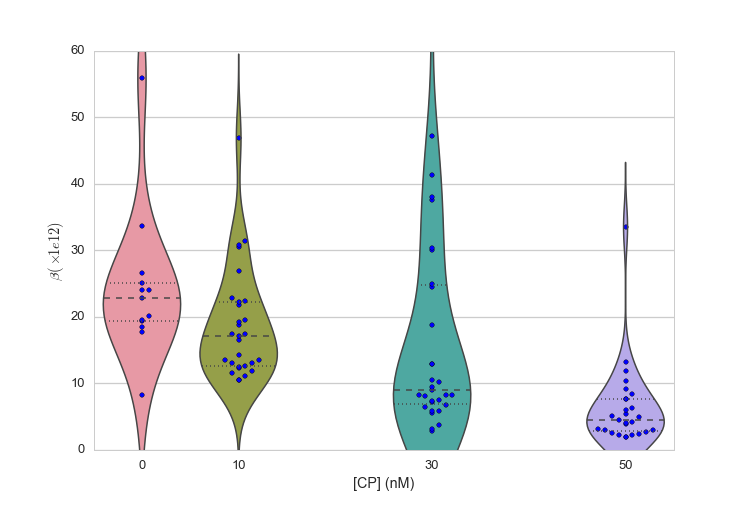
\includegraphics[width=0.800\linewidth]{beta_violin.png}
\caption{Violin plot showing the repartition of the prefactor with the quantity of
Capping Protein. Decrease of prefactor with increasing amount of Capping
Protein indicates a lower force between the probe bead and the actin bead
for the same corrected distance between bead centers.}\label{index-latex:beta-violin}\end{figure}

The last parameter of our model is \(\delta\), the distance at which the force
diverges.   It can be seen in \hyperref[index-latex:delta-violin]{Figure  \ref*{index-latex:delta-violin}} that with the exception
of zero Capping Protein, the distance at which the model diverges gets
closer to the diameter of the polystyrene bead as the concentration of Capping
Proteins in the medium increases. It is interesting to see that the distance offset
\(\delta\) is very close from the bead diameter in the absence of Capping Protein, when no
biomimetic actin cortices forms.
\begin{figure}[htbp]
\centering
\capstart

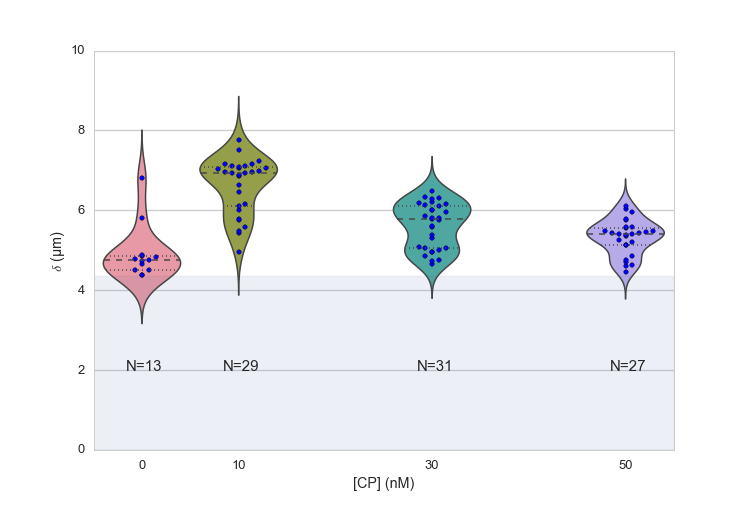
\includegraphics[width=0.800\linewidth]{delta_violin.png}
\caption{Violin plot showing the variation of the offset distance \(\delta\)
with the Capping Protein concentration. The shaded area represents the
non-physical region which would correspond to a diverging force beyond the
contact of the two polystyrene beads. Experimental data with \(\delta\)
value in this regions have been excluded from further analysis.}\label{index-latex:delta-violin}\end{figure}


\subsection{Determination of Young's Modulus}
\label{index-latex:determination-of-young-s-modulus}
To determine the mechanical properties of the gel between the actin and the
probe bead, we model it as a purely elastic material. The viscous effects are
neglected in the approach part as the approach at different speed show no
clear effect on the approach curves (\hyperref[index-latex:many-speed]{Figure  \ref*{index-latex:many-speed}}). We consider
the compression of the material between the two beads. The surface of the
compressed material is approximated by the projected surfaces of the bead along the
direction of compression (\(\pi R^2\)).  The thickness of the compressed
material is taken as being the distance between bead centers corrected by the
distance offset \(\delta\) as any material below delta can be considered as
infinitively rigid for the optical tweezer.

The stress exerted onto the material projected onto the bead surface or radius
\(R\) can be written :
\phantomsection\label{index-latex:equation-eqa32}\begin{gather}
\begin{split}\sigma = \frac{F}{\pi R^2}\end{split}\label{index-latex-eqa32}
\end{gather}
For small deformation the local strain of the material \(u\) can be written
as a function of the corrected bead position \(d_c\) and the considered location
along the axis between the two bead center \(x\) :
\phantomsection\label{index-latex:equation-eqa33}\begin{gather}
\begin{split}u(x)= \frac{d_c-x}{d_c}\end{split}\label{index-latex-eqa33}
\end{gather}
We can express the local differential strain around the position \(d_c\) of the
bead : \(\partial u = -\partial x/ \partial d_c\) in which the minus sign
reflect the choice of the coordinate system: a decrease in \(x\) with a
positive Young's modulus \(E\) should lead to an increase of the exerted force.
The locally felt Young's modulus
at the distance \(d_c\) is then
\phantomsection\label{index-latex:eq-e}\phantomsection\label{index-latex:equation-eqa34}\begin{gather}
\begin{split}E(d_c) = \left.\frac{\partial\sigma}{\partial u}\right|_{d_c}\end{split}\label{index-latex-eqa34}
\end{gather}
By injecting the expression of \(u\) and \(\sigma\) this lead to :
\phantomsection\label{index-latex:equation-eqa35}\begin{gather}
\begin{split}E(d_c) &= -\frac{d_c}{\pi R^2}\times \Big(\frac{dF}{dx}\Big) \Big|_{x=d_c}\\
     &= E_0 d_c^\alpha\end{split}\label{index-latex-eqa35}
\end{gather}
In which the value of \(E_0\) can be expressed as function of the power law exponent \(\alpha\) and the prefactor \(\beta\) :
\phantomsection\label{index-latex:equation-eqa36}\begin{gather}
\begin{split}E_0 = - \frac{\alpha\beta}{\pi R^2}\end{split}\label{index-latex-eqa36}
\end{gather}
Experimentally, the probed Young's modulus corresponds to the average mechanical
properties of the actin cloud between the surface of the actin bead and the
surface of the probe bead and do not reflect the variation of the mechanical
properties of the uncompressed actin cloud with position.
Physically \(E_0\) correspond to the Young's modulus as a corrected distance of \(d_c = 1 \mu{}m\)
(See \hyperref[index-latex:ev]{Fig  \ref*{index-latex:ev}})
The geometry of the
system and the fluorescence signal suggest a decrease of the density of the
actin cloud with the distance from the actin-bead center. All values
reported later represent estimation of elasticity of an effective Young's
modulus. The value of this effective Young's modulus are 3 orders of magnitude
smaller than the known elasticity of dendritic gels formed on beads that has been measured to be in the
order of kPa {\hyperref[index-latex:marcy2004]{{[}Marcy, Prost, Carlier, Sykes,  2004{]}}}.

This difference in elasticity might explain why the mechanical actions of this actin cloud as not been
seen before in other measurement like micro-pipette aspiration,
micro needle deformation or Atomic Force Microscopy indentation that have
sensitivities in the order of nN while the forces exerted by this actin cloud
are in the order of pN.

Nonetheless, {\hyperref[index-latex:gardel2003]{{[}Gardel, Valentine, Crocker,  et al.  2003{]}}} show that such low moduli can be obtain using
sparse entangle actin network, and confirm the idea that the actin-cloud seen
with the optical-tweezer indent experiments has a fundamentally different
structure than the dense dendritic network on the actin
bead surface.
\begin{figure}[htbp]
\centering
\capstart

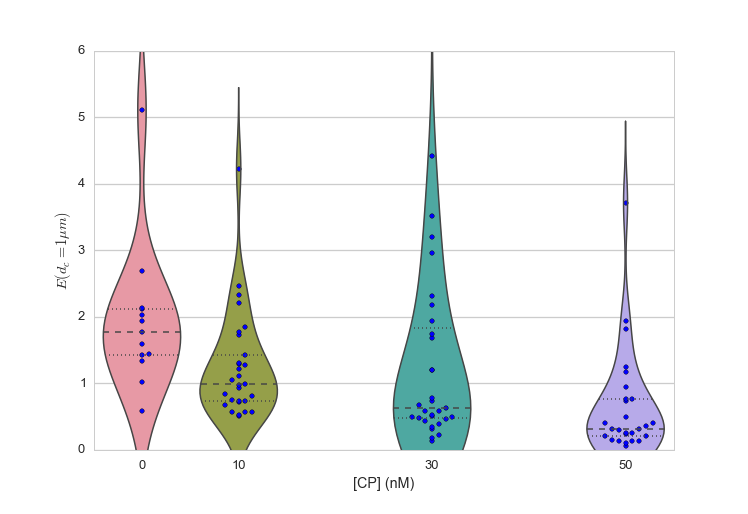
\includegraphics[width=0.800\linewidth]{E0_violin.png}
\caption{Young's Modulus prefactor as a function of Capping Protein show a decrease of
average Young's modulus with an increase of Capping Protein concentration.}\label{index-latex:ev}\end{figure}


\subsection{Mechanical properties}
\label{index-latex:mechanical-properties}
To investigate the mechanical properties of the network that should arise from
a \(\alpha = -1\) power law, we model the deformation of the actin cloud by
the theory of semi-flexible entangled polymer networks ({\hyperref[index-latex:isambert1996]{{[}Isambert, Maggs,  1996{]}}},
{\hyperref[index-latex:mackintosh1995]{{[}MacKintosh, Kas, Janmey,  1995{]}}}, {\hyperref[index-latex:morse1998a]{{[}Morse,  1998a{]}}}).

The Young's modulus of semi-flexible filaments in a 3D environment can be
expressed as a function of filament contour length density \(\rho\) and the
entanglement length \(L_e\) as {\hyperref[index-latex:morse1998b]{{[}Morse,  1998b{]}}}:
\phantomsection\label{index-latex:equation-eqa37}\begin{gather}
\begin{split}E= \frac{2.(1+\nu).7.k_BT \rho}{5L_e}\end{split}\label{index-latex-eqa37}
\end{gather}
In which \(\nu\) is the Poisson ratio that allows the conversion from shear to
elastic modulus. Previous studies have investigated the non-linear stiffening of
such actin network for large deformation {\hyperref[index-latex:semmrich2008]{{[}Semmrich, Larsen, Bausch,  2008{]}}} and found that in
our condition, the linear description of theses networks holds to describe the
actin-cloud.

Similar to {\hyperref[index-latex:morse1998a]{{[}Morse,  1998a{]}}} we express the entanglement length as a
function of persistence length and filament density: \(L_e\approx L_p^{1/5} \rho^{-2/5}\). We can
reduce the expression of the Young's modulus to a function of the following
parameters :
\begin{itemize}
\item {} 
The Poisson Ratio \(\nu\),

\item {} 
The persistence length of actin filaments \(L_p\)

\item {} 
The mesh size of the network \(\xi_0^2 = \rho_0\)

\item {} 
The ``size'' of the cloud, for which we use the distance at which the force
is first significant \(d_0\)

\end{itemize}

We need also to consider that for a general compressible material, the
only variable that changes during compression is the density \(\rho\)
which can be expressed as a function of the corrected distance \(\rho \to
\rho(d_c)\)

Thus leading to :
\phantomsection\label{index-latex:equation-eqa}\begin{gather}
\begin{split}E(d_c)=\frac{ (1+\nu).14.k_BT}{5L_p^{1/5}}\times \rho(d_c)^{7/5}\end{split}\label{index-latex-eqa}
\end{gather}
The scaling exponent of \(E\) in equation \eqref{index-latex-eqa} with \(d_c\) should match the exponent
of the experimentally found power law \(\alpha\). Thus the density can be
expressed in the following form :
\phantomsection\label{index-latex:equation-eq-rho}\begin{gather}
\begin{split}\rho(d_c)=\rho_0(d_c/d_0)^{5/7\times\alpha}\end{split}\label{index-latex-eq-rho}
\end{gather}
By the definition of \(\rho\) in {\hyperref[index-latex:morse1998a]{{[}Morse,  1998a{]}}} which is
the filament contour length per unit volume, we can determine the
mesh-size \(\xi_0\) of the undeformed network:
\phantomsection\label{index-latex:equation-eqa38}\begin{gather}
\begin{split}\xi_0 = 1/\sqrt\rho_0\end{split}\label{index-latex-eqa38}
\end{gather}
By comparing this to the phenomenological fit we can express the elastic
modulus as a function of the distance and the mesh size, as a function of the
fit parameters and characteristic scales of the system.
\phantomsection\label{index-latex:equation-eqb}\begin{gather}
\begin{split}E(d_c)     &=  \frac{(1+\nu).14.k_BT}{5L_p^{1/5}\xi_0^{14/5} \left.d_0\right.^{\alpha}}\times \left.d_c\right.^{\alpha}.\\
                &=  E_0' \times \left.d_c\right.^{\alpha}\end{split}\label{index-latex-eqb}
\end{gather}
In which \(E_0'\) can be identified as \(E_0\) in \eqref{index-latex-eqa} to extract the
closed form solution for the mesh size \(\xi_0\) :
\phantomsection\label{index-latex:equation-eqa39}\begin{gather}
\begin{split}\xi_0=\left(-\frac{({2-\frac{5}{7}\alpha)}.k_BT\pi R^2}{5\alpha \beta L_p^{\frac{1}{5}}\left.d_0\right.^{\alpha}}\right)^{\frac{5}{14}}\end{split}\label{index-latex-eqa39}
\end{gather}
The found mesh size is in the order of 0.3 to 0.4 µm which is consistent with previous findings
:\emph{Morse1998b}. The variation of the
mesh size can be seen on \hyperref[index-latex:xi-violin]{figure  \ref*{index-latex:xi-violin}} and does not seem to have a
correlation with the concentration of Capping Protein.
\begin{figure}[htbp]
\centering
\capstart

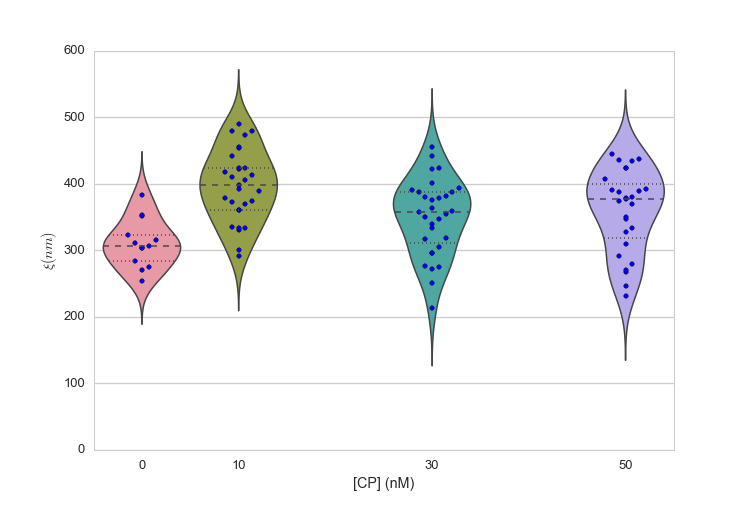
\includegraphics[width=0.800\linewidth]{xi_violin.png}
\caption{Meshsize vs Capping plot.}\label{index-latex:xi-violin}\end{figure}

We explore the correlation between the mesh size and \(\delta\) by plotting  the mesh size again the distance offset \(\delta\) (\hyperref[index-latex:dxcf]{Fig  \ref*{index-latex:dxcf}}).
\hyperref[index-latex:dxf]{Figure  \ref*{index-latex:dxf}} shows the relation between the mesh size and the offset
distance \(\delta\) independently for each concentration of Capping Protein.
\begin{figure}[htbp]
\centering
\capstart

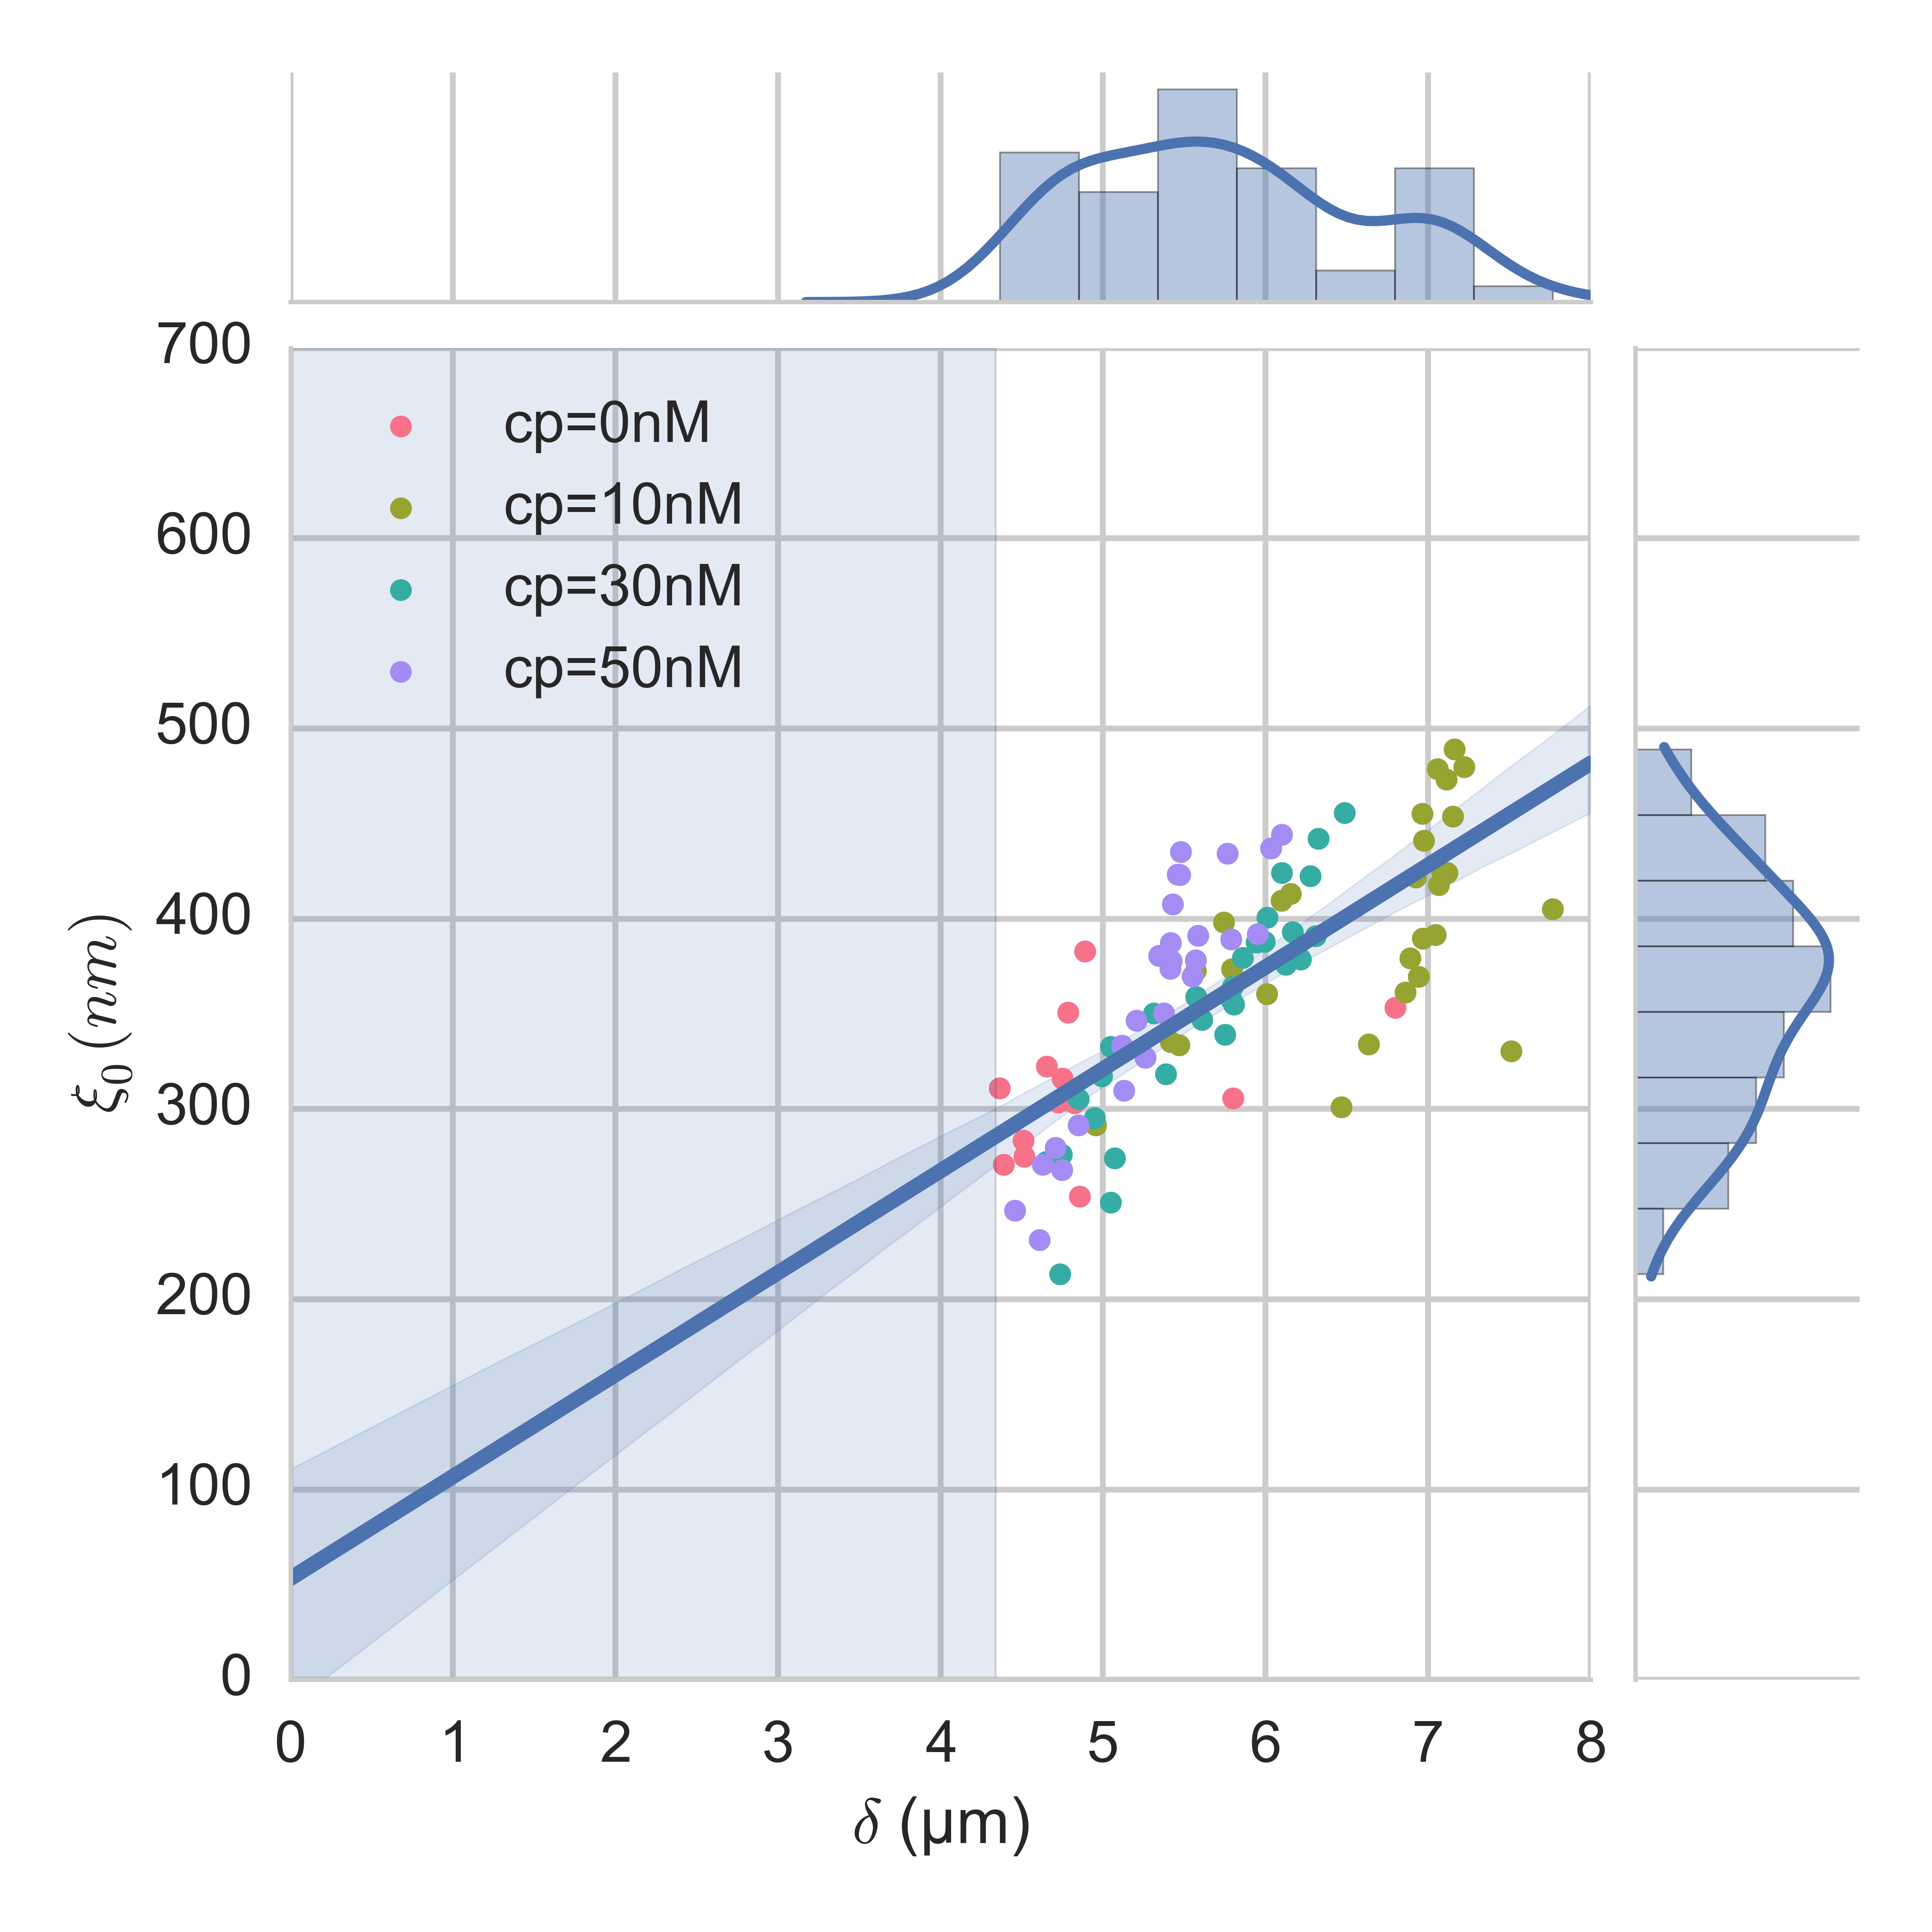
\includegraphics[width=1.000\linewidth]{delta-xi-corr.png}
\caption{Correlation of the meshsize \(\xi_0\) with the distance offset \(\delta\),
with marginal distribution as histogram on the side and on the top.  Shaded
regions represent confidence interval at 95\%.}\label{index-latex:dxcf}\end{figure}
\begin{figure}[htbp]
\centering
\capstart

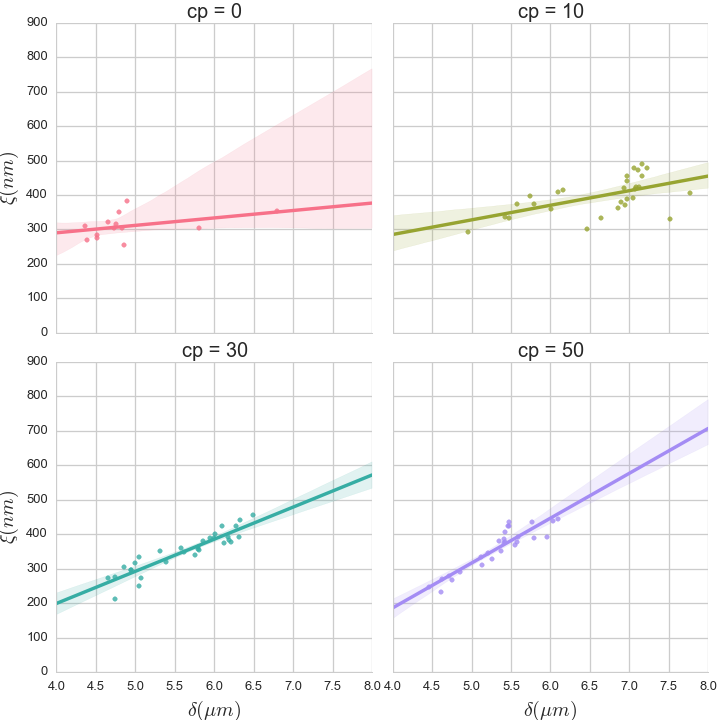
\includegraphics[width=1.000\linewidth]{delta-xi-facets.png}
\caption{Same figure as \hyperref[index-latex:dxcf]{Fig  \ref*{index-latex:dxcf}} for each concentration of Capping Protein,
with linear regression and confidence intervals at 95\%.}\label{index-latex:dxf}\end{figure}

From \eqref{index-latex-eqa} and \eqref{index-latex-eqb} by identifying the prefactor it is also possible
to extract the Poisson ratio (\(\nu\)) of the compressed material :
\phantomsection\label{index-latex:equation-nu=f(alpha)}\begin{gather}
\begin{split}\nu =\frac 1 2 \times \left( \frac 5 7.\alpha +1\right)\end{split}\label{index-latex-nu=f(alpha)}
\end{gather}
The Poisson ratio depends only on the powerlaw exponent and thus varies little
with the amount of Capping Protein concentration.  We found value of the
Poisson ratio that are between 0.1 and 0.2 corresponding to compressible
foam-like materials that do not expand highly in the direction orthogonal to
the compression axis. Previous study of bulk actin network find a Poisson
ration of 0.5 (incompressible material) for actin concentration of 21.5 µM.  We
suspect that the low actin concentration used in our experiments (4µM) is the
reason for the low Poisson Poisson Ratio. Also the local structure of filaments
emanating from the  bead may explain the large compressibility of our actin
cloud.


\subsection{Interpretation}
\label{index-latex:interpretation}
The results of our data analysis lead to the interpretation that
a dense actin gel of elasticity close to \textasciitilde{}1kPa is polymerized
on the surface of the actin bead. This stiff gel
cannot be indented by the optical tweezer. Beyond this dense gel a soft
actin cloud with an effective elastic modulus of 1 Pa and below is
present and extends on distances that are several times bigger than the thickness
of the reconstituted actin cortex (\hyperref[index-latex:fig-interpretation]{Fig  \ref*{index-latex:fig-interpretation}}). The
structure of this actin cloud is expected to be quite different from the
dendritic gel and be mostly constituted of loosely entangle actin filaments.

In this model, the offset distance \(\delta\) correspond to the limit of the dense
dendritic actin network mimicking the actin cortex that grows on actin beads.
The high elastic modulus of this gel makes it impenetrable by the small forces generated by the optical tweezer we use. The
value of \(\delta\) we found are coherent with the measured thickness \(e
\simeq \delta - 2.R_{bead}\) of the  biomimetic actin cortex as measured by
epifluorescence in {\hyperref[index-latex:kawska2012]{{[}Kawska, Carvalho, Manzi,  et al.  2012{]}}} and found to be in the range of 1 to 2 µm. The decrease
of \(\delta\) with Capping Protein is also coherent with the decrease of gel
thickness.

The filaments composing the actin cloud emanate directly from the actin
cortex in which the nucleation of actin polymerisation started at the surface
of the bead. Eventually, a few filaments can escape from the network and are
capped by the Capping Protein only when the growing extremity is already several
micrometers from the bead surface.
\begin{figure}[htbp]
\centering
\capstart

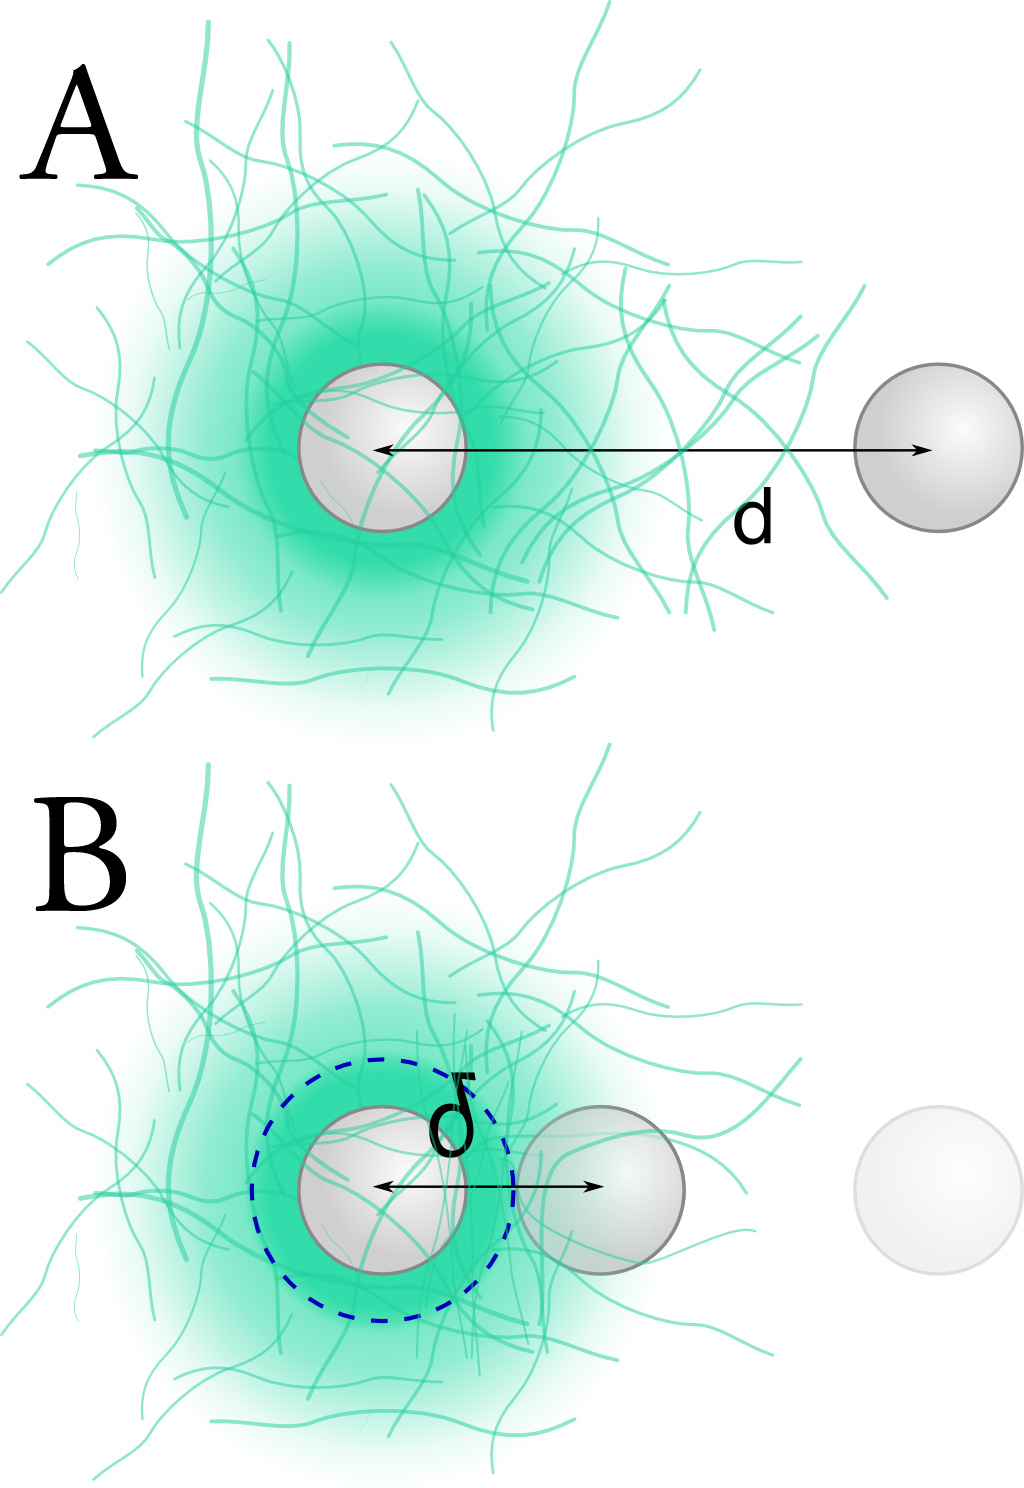
\includegraphics[width=0.900\linewidth]{interp-delta.png}
\caption{A ) Schematic of an actin cloud. Left:  The actin bead triggers actin
polymerisation. Right Probe Bead. On the surface of the actin bead a dense
and dendritic network forms a biomimetic actin cortex with an elastic
modulus close to the kPa (Dark Green). From this actin cortex emanates a
softer actin structure : The actin cloud . The actin cloud is a loosely
entangled network formed by the filaments escaping from the bead's actin
cortex and extending over several micrometers. The actin cloud has an average
elastic modulus which is several order of magnitude softer than the actin
cortex. B ) From the point of view of the probe bead in optical tweezer, the
system (actin-bead+actin cortex) behave as a hard-sphere of radius
\(\delta-R\)}\label{index-latex:fig-interpretation}\end{figure}

The thickness of the actin cortex \(e\) as measured in {\hyperref[index-latex:kawska2012]{{[}Kawska, Carvalho, Manzi,  et al.  2012{]}}}
increases with time during the polymerisation of actin. We can predict that the
offset distance \(\delta\) should increase with time, except in the absence of
Capping Protein where no actin cortices form. This can be verified on
\hyperref[index-latex:time-delta-corr]{figure  \ref*{index-latex:time-delta-corr}} that shows the evolution of \(\delta\) as a function
of polymerisation time.
\begin{figure}[htbp]
\centering
\capstart

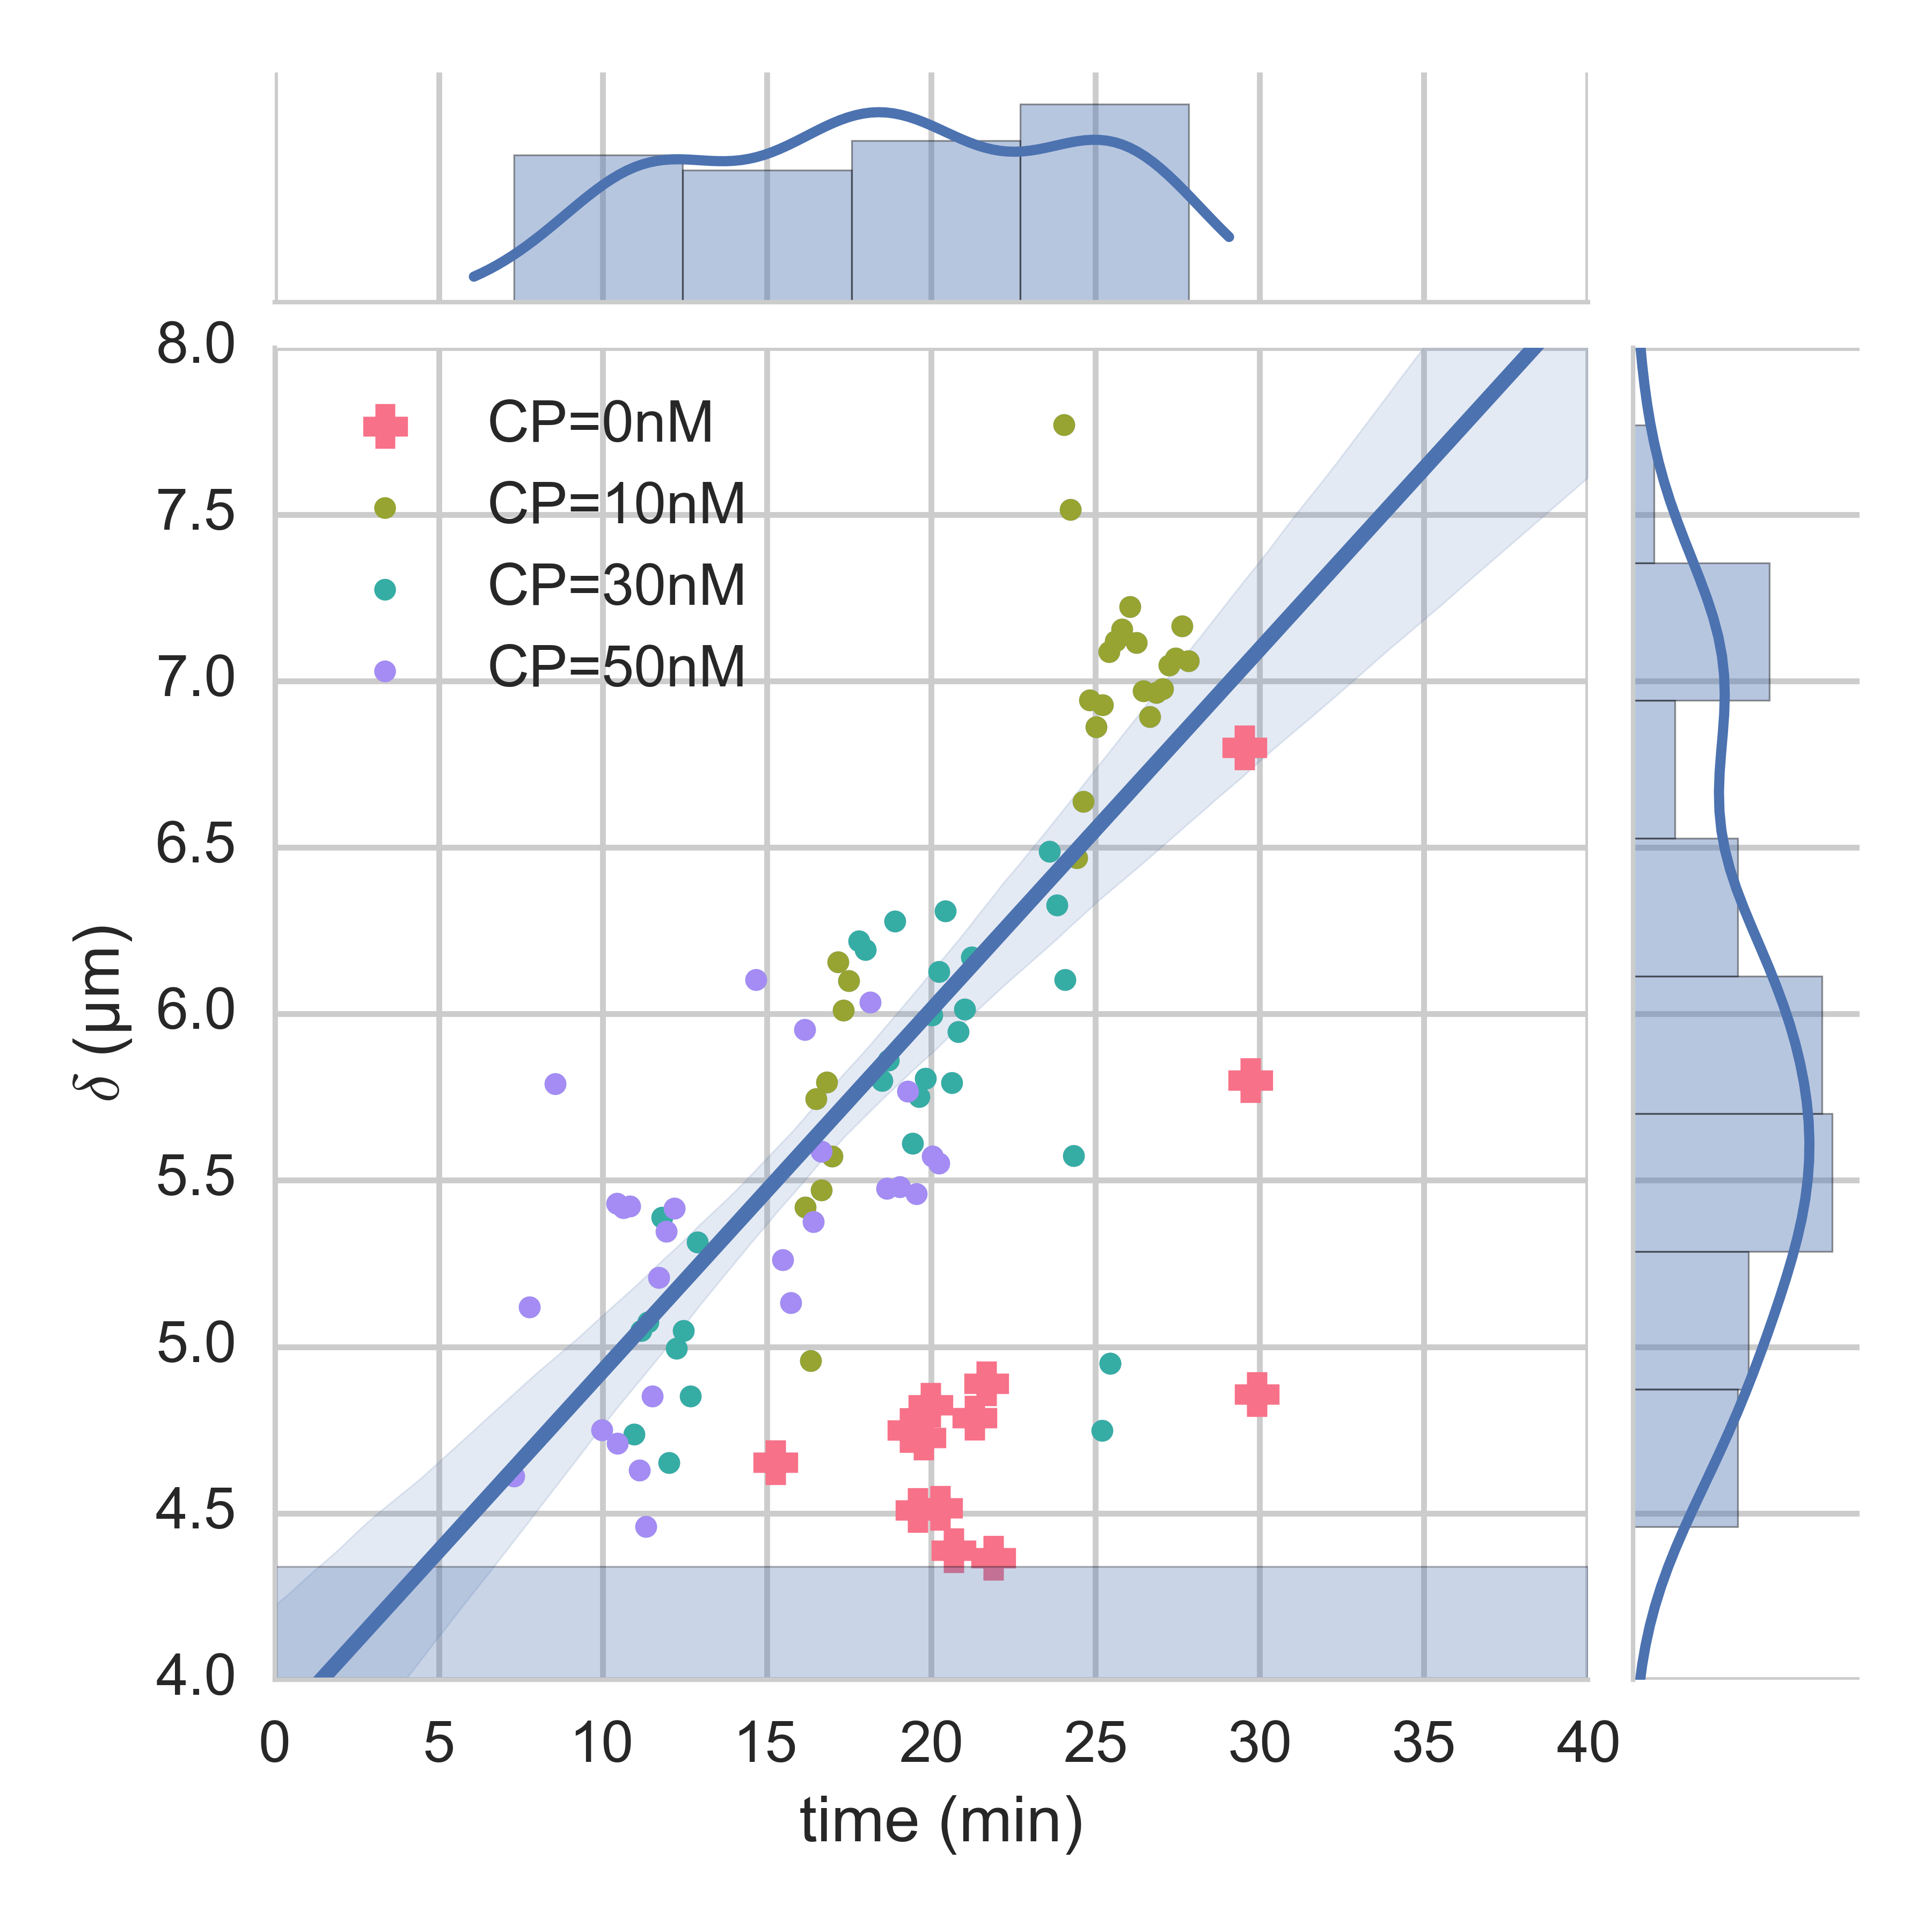
\includegraphics[width=0.900\linewidth]{time-delta-corr.png}
\caption{Distance offset \(\delta\) as a function of time (min) since mix of actin, ATP
and beads. Linear fit with confidence interval at 95\% (light shaded area)
and bead surface (dark shaded area). Samples taken in the absence of Capping
Protein are not taken into account in the regression (Pink +). The increase
of \(\delta\) with time is coherent with the measured increase of the gel
thickness \(e\) as measured in {\hyperref[index-latex:kawska2012]{{[}Kawska, Carvalho, Manzi,  et al.  2012{]}}}}\label{index-latex:time-delta-corr}\end{figure}


\section{Relaxation phase}
\label{index-latex:id29}
The approach phase of the indentation cycle has been modeled with a purely
elastic mode. However, the force distance plot shows a significant dissipation
marked by an hysteresis \hyperref[index-latex:force-distance]{Fig  \ref*{index-latex:force-distance}}. The repetitive indent cycle giving the same
force-distance curves (\hyperref[index-latex:reproc]{Fig  \ref*{index-latex:reproc}}) allow to exclude a plastic deformation.
We can hence reject the hypothesis of ruptures of the
actin meshwork or breakage near the entanglement points.

The theory of entangled filaments networks that allowed us to understand the link between the phenomenological
model and the mechanical properties of the network also proposes a relation to
explain the relaxation of the network.

In this model {\hyperref[index-latex:morse1998a]{{[}Morse,  1998a{]}}}, the visco elastic modulus  \(E\) is a function of time
and can be written as \(E(t) = E\times \chi(t)\) with
\phantomsection\label{index-latex:equation-chi}\begin{gather}
\begin{split}\chi(t)=\sum_{n, odd} \frac{8}{n^2 \pi^2}exp\left(- \frac{n^2\pi^2 t}{ \tau_{rep}} \right)\end{split}\label{index-latex-chi}
\end{gather}
In which \(\tau_{rep} = \frac{l_f^2}{D_{rep}}\) is a single fit parameter
that depends on diffusion constant for filament reptation \(D_{rep}\) and the
filaments length \(l_f\). In this form, \(\chi\) is a sum of
exponential decays with well defined characteristic timescales and amplitudes
that decrease as \(1/n^2\). To fit this model to the data of the
relaxation phase, we can limit ourselves to the first 40 terms of the sum as
any of the subsequents terms represent timescales we cannot reach with our
experimental resolution.

It should be noted that the value of \(\chi(t=0)\) is 1 and should be
treated particularly in order to insure continuity of the force applied on the
actin-bead in the model.

Using this sum of exponential decays is coherent with the common findings of
power-laws found in the frequency-dependant shear modulus of both \emph{in vivo} and \emph{in vitro} actin
networks as well as the relaxation behavior found in cells.

In order to determine \(\tau_{rep}\), the Young's modulus determined in the
approach phase is used and the model is fitted against the relaxation data.  A
result of such a fit can be seen on \hyperref[index-latex:fit-3-phases]{figure  \ref*{index-latex:fit-3-phases}}. The value of
\(\tau_{rep}\) are highly variable and the fit can be difficult when the relaxation is
slow or in the order of the measured noise. Variation of \(\tau_{rep}\) with the
concentration in Capping Protein can be seen on \hyperref[index-latex:tau-violin]{figure  \ref*{index-latex:tau-violin}}, and
one example of fit on the \hyperref[index-latex:fit-3-phases]{figure  \ref*{index-latex:fit-3-phases}}
\begin{figure}[htbp]
\centering
\capstart

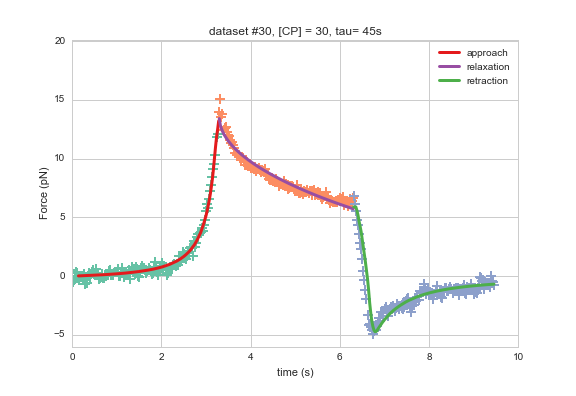
\includegraphics[width=0.800\linewidth]{3phases.png}
\caption{Force as a function of time as well as fit for the 3 phases, approach,
relaxation and retraction.}\label{index-latex:fit-3-phases}\end{figure}
\begin{figure}[htbp]
\centering
\capstart

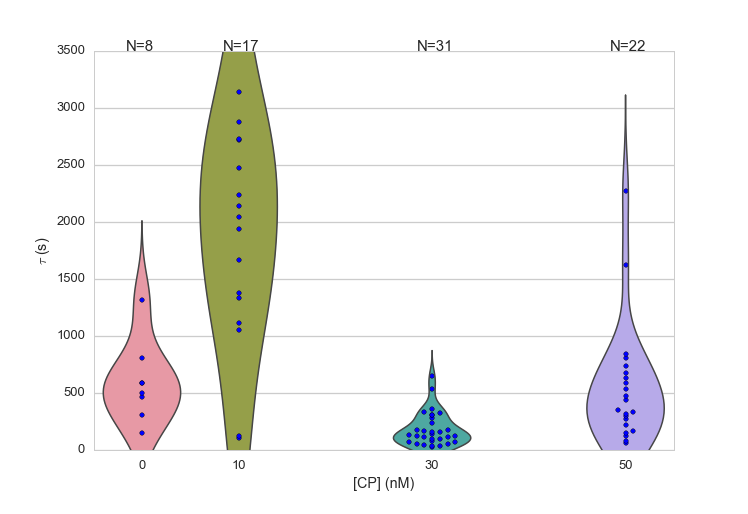
\includegraphics[width=0.800\linewidth]{tau_violin.png}
\caption{Violin plot showing the repartition of \(\tau_{rep}\) as a function of capping
protein. Outlier (\(\tau_{rep}\) negative or greater than tens of minutes removed)}\label{index-latex:tau-violin}\end{figure}

We can see here that the polymer model introduced in {\hyperref[index-latex:morse1998a]{{[}Morse,  1998a{]}}} allows
to completely fit the succession of approach and relaxation phases.  To check if
the fit parameters give realistic value, we can estimate the diffusion constant
for filament reptation \(D_{rep}\).
\phantomsection\label{index-latex:equation-eqa3-10}\begin{gather}
\begin{split}D_{rep} &= \frac{k_bT}{\gamma l_f} \\\end{split}\label{index-latex-eqa3-10}
\end{gather}
In which \(\gamma\approx {2\pi\eta_s}/{ln(\xi_0/d_f)}\) is the friction
coefficient per unit length. \(\gamma\) depends on the solvent viscosity
\(\eta_s\), the mesh-size \(\xi_0\) and the filament diameter
\(d_f\) (\(~7nm\) for actin).  We use \(\eta_s=10^{-3} Pa\times s\)
for water and a mesh size in the order of 400nm as determined from the approach phase
(\hyperref[index-latex:tau-violin]{Fig  \ref*{index-latex:tau-violin}}). Using \(\tau_{rep}\) given by the fit, this lead to filaments
length ranging from 3 to 8 µm, which is consistent with TIRF experiments and simulation as done in {\hyperref[index-latex:kawska2012]{{[}Kawska, Carvalho, Manzi,  et al.  2012{]}}}.


\subsection{Retraction Phase}
\label{index-latex:retraction-phase}
During the retraction phase the force decreases, becomes negative after a
retraction of 3 to 4 µm, and show a slow  return to 0 at large distance.
Sticking events can be seen when the force becomes abruptly negative before
relaxing as fast. \hyperref[index-latex:sticking-event]{Figure  \ref*{index-latex:sticking-event}} shows such a sticking even
happening during an indentation cycle.
\begin{figure}[htbp]
\centering
\capstart

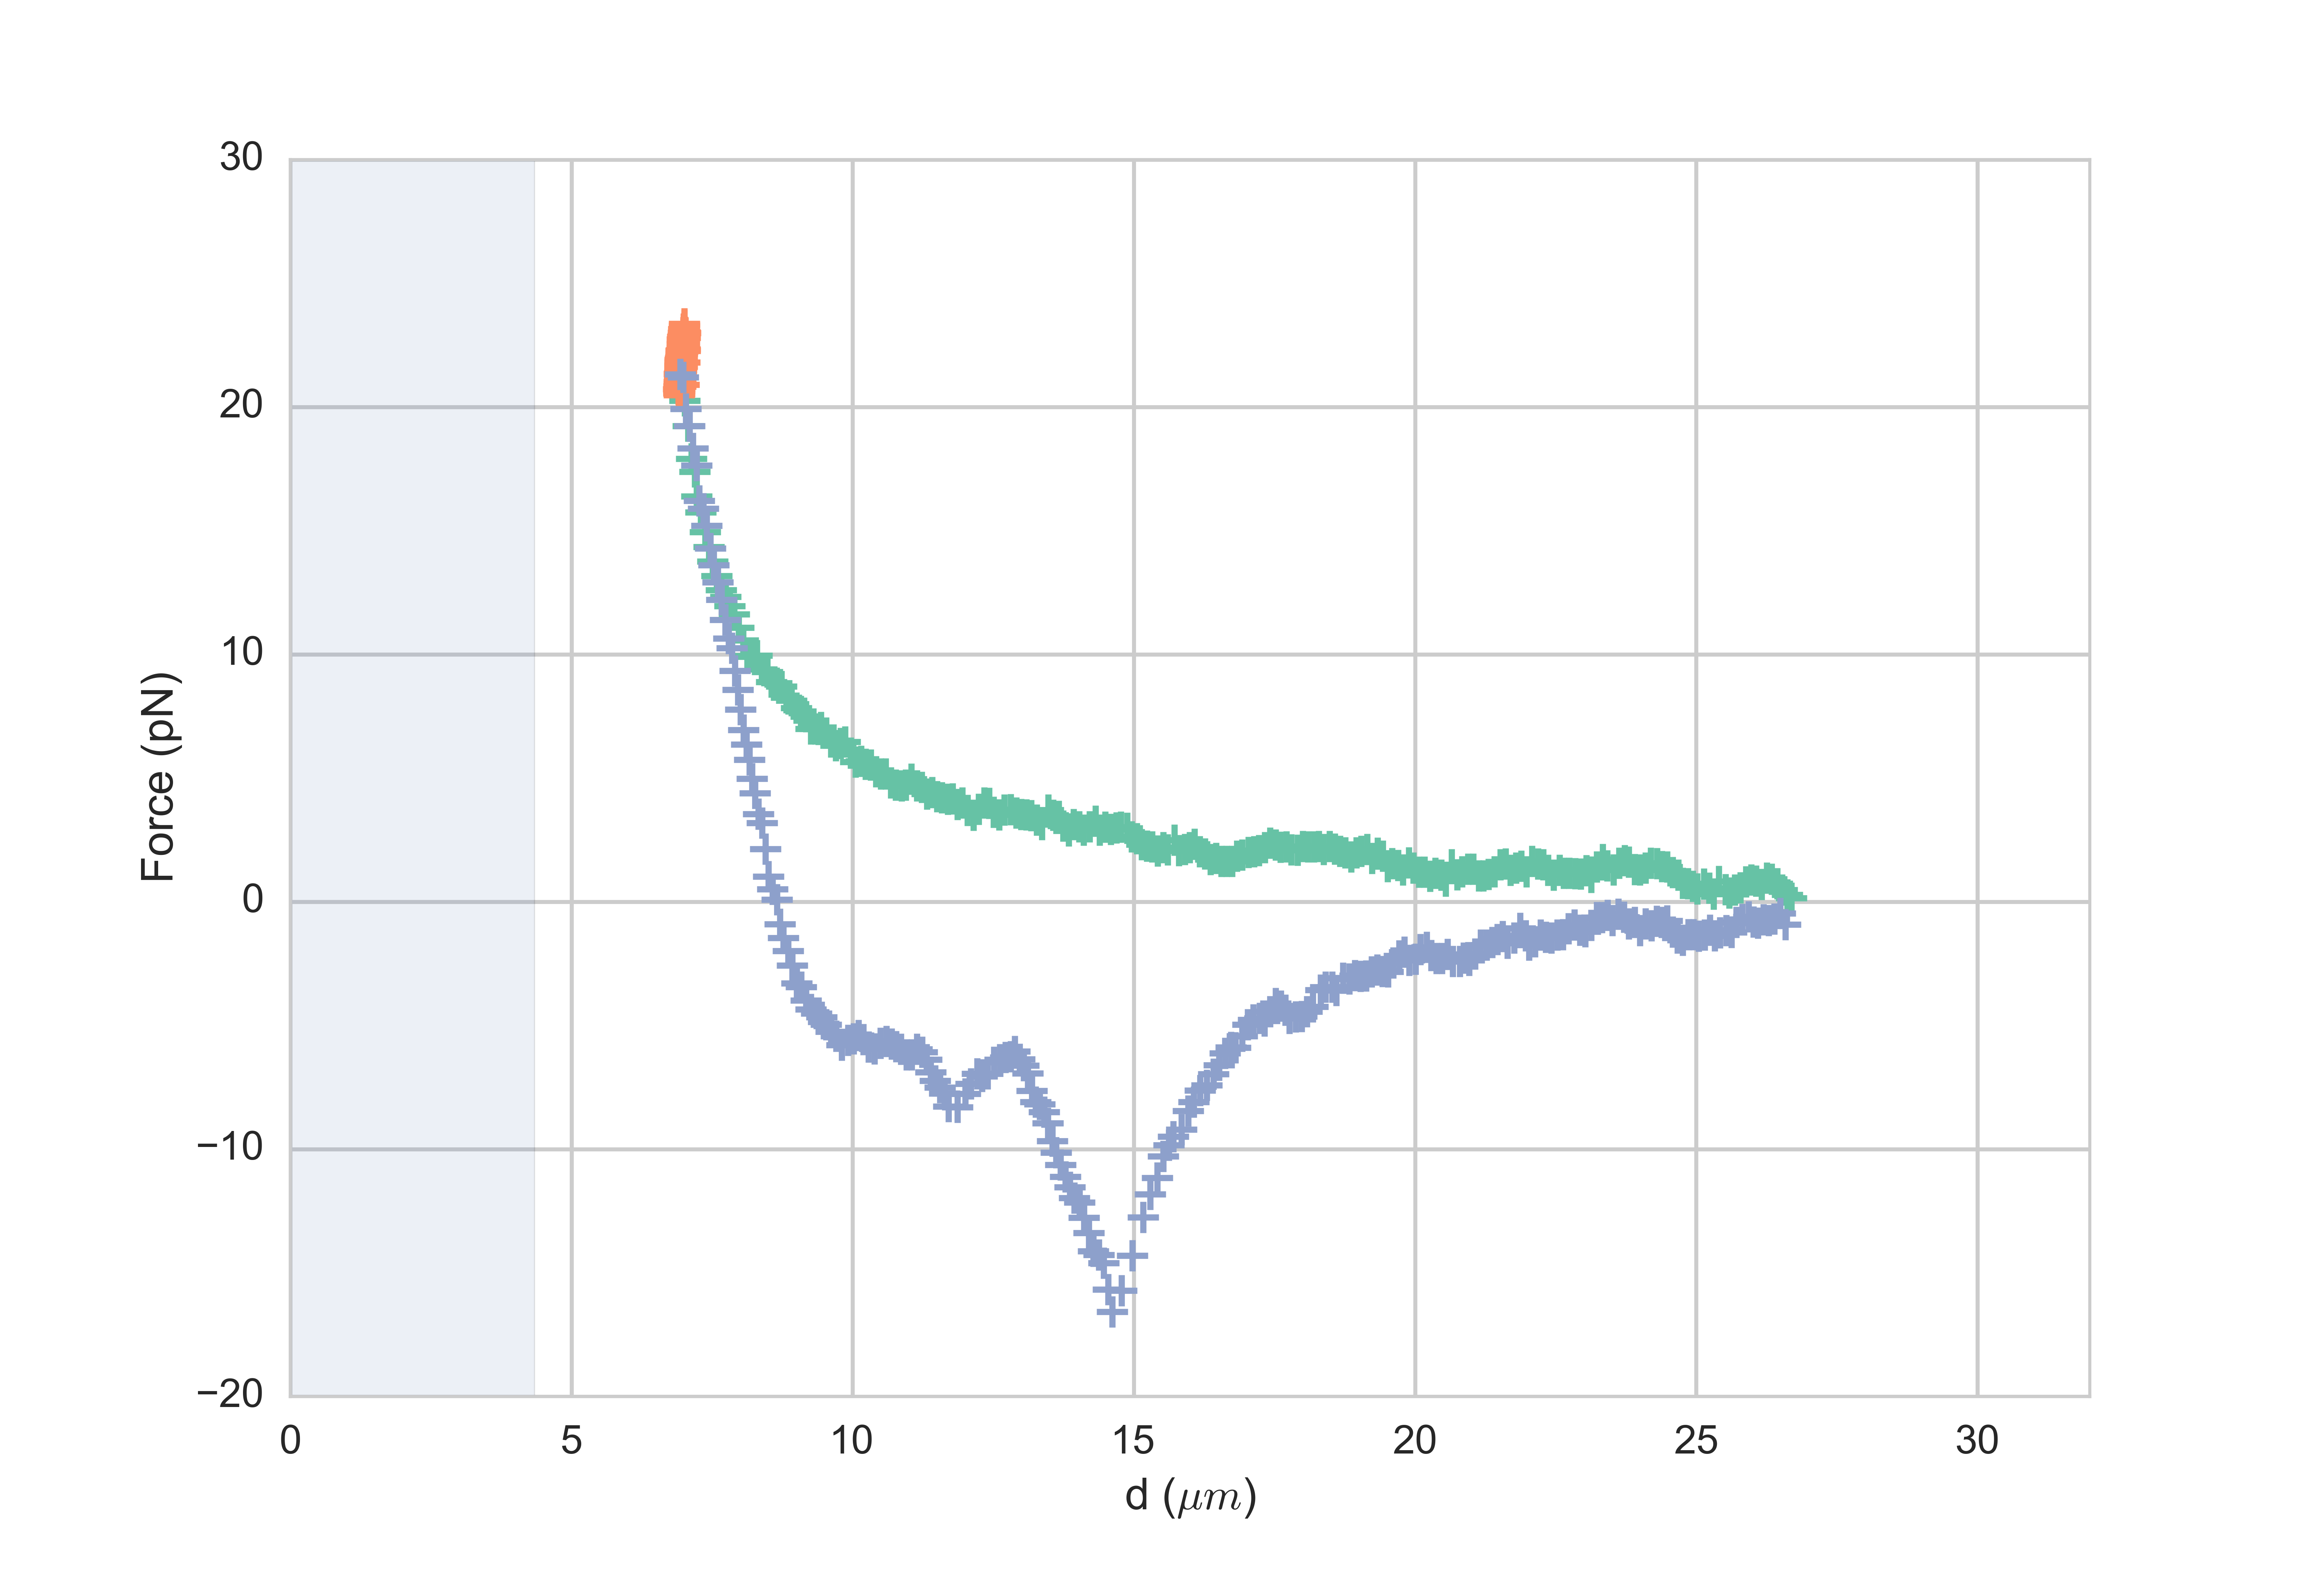
\includegraphics[width=0.800\linewidth]{sticking-event.png}
\caption{A sticking event at \(d=15\mu{}m\) where the force can be seen decreasing rapidly
up to -18 pN before quickly returning to its normal value. A second smaller
sticking even is present at \(d=12\mu{}m\) Sticking even appear roughly 20\% of
the experiments.}\label{index-latex:sticking-event}\end{figure}

We assume that the sticking events are characteristic to non-specific interaction
between the probe bead and the actin cloud.  In the case when no sticking event
is present, we assume partial closing of the actin cloud beyond the
probe bead during the relaxation phase and model the retraction curve as a
transition between the damped-approach curve and a penetration of the probe
bead through the closing actin cloud.

During the approach phase the force exerted on the actin-bead is
\(F(d)=\beta(d-\delta)^\alpha\). During the relaxation phase the force
decrease from \(F(t_1)\) to \(F(t_2)\) with the relation :
\phantomsection\label{index-latex:equation-eqa311}\begin{gather}
\begin{split}\frac{F(t_2)}{F(t_1)} = \chi(t_2-t_1)\end{split}\label{index-latex-eqa311}
\end{gather}
We can write that the force exerted on the actin-bead during the retraction can
be written as a sum of the force felt during the approach, damped during the
relaxation (\(F_{da}\)), plus a force due to the closing of the actin
network behind the bead \(F_{closing}\).
\phantomsection\label{index-latex:equation-eqa312}\begin{gather}
\begin{split}F_{ret}(d) &= F_{da}(d) + F_{closing}(d)\\
F_{ret}(d) &= \chi(t_2-t_1).\beta(d-\delta)^\alpha+ F_{closing}(d)\end{split}\label{index-latex-eqa312}
\end{gather}
\(F_{closing}\) is computed using the fit parameter \(\alpha\), \(\beta\), \(\delta\) and \(\tau_{rep}\) (\hyperref[index-latex:retract-powerlaw]{Fig  \ref*{index-latex:retract-powerlaw}}).

On a double logarithmic scale and at long distance \(F_{closing}\) also seem to
follow a power law (\(F_{plaw}\)), when no sticking events are present.
\begin{figure}[htbp]
\centering
\capstart

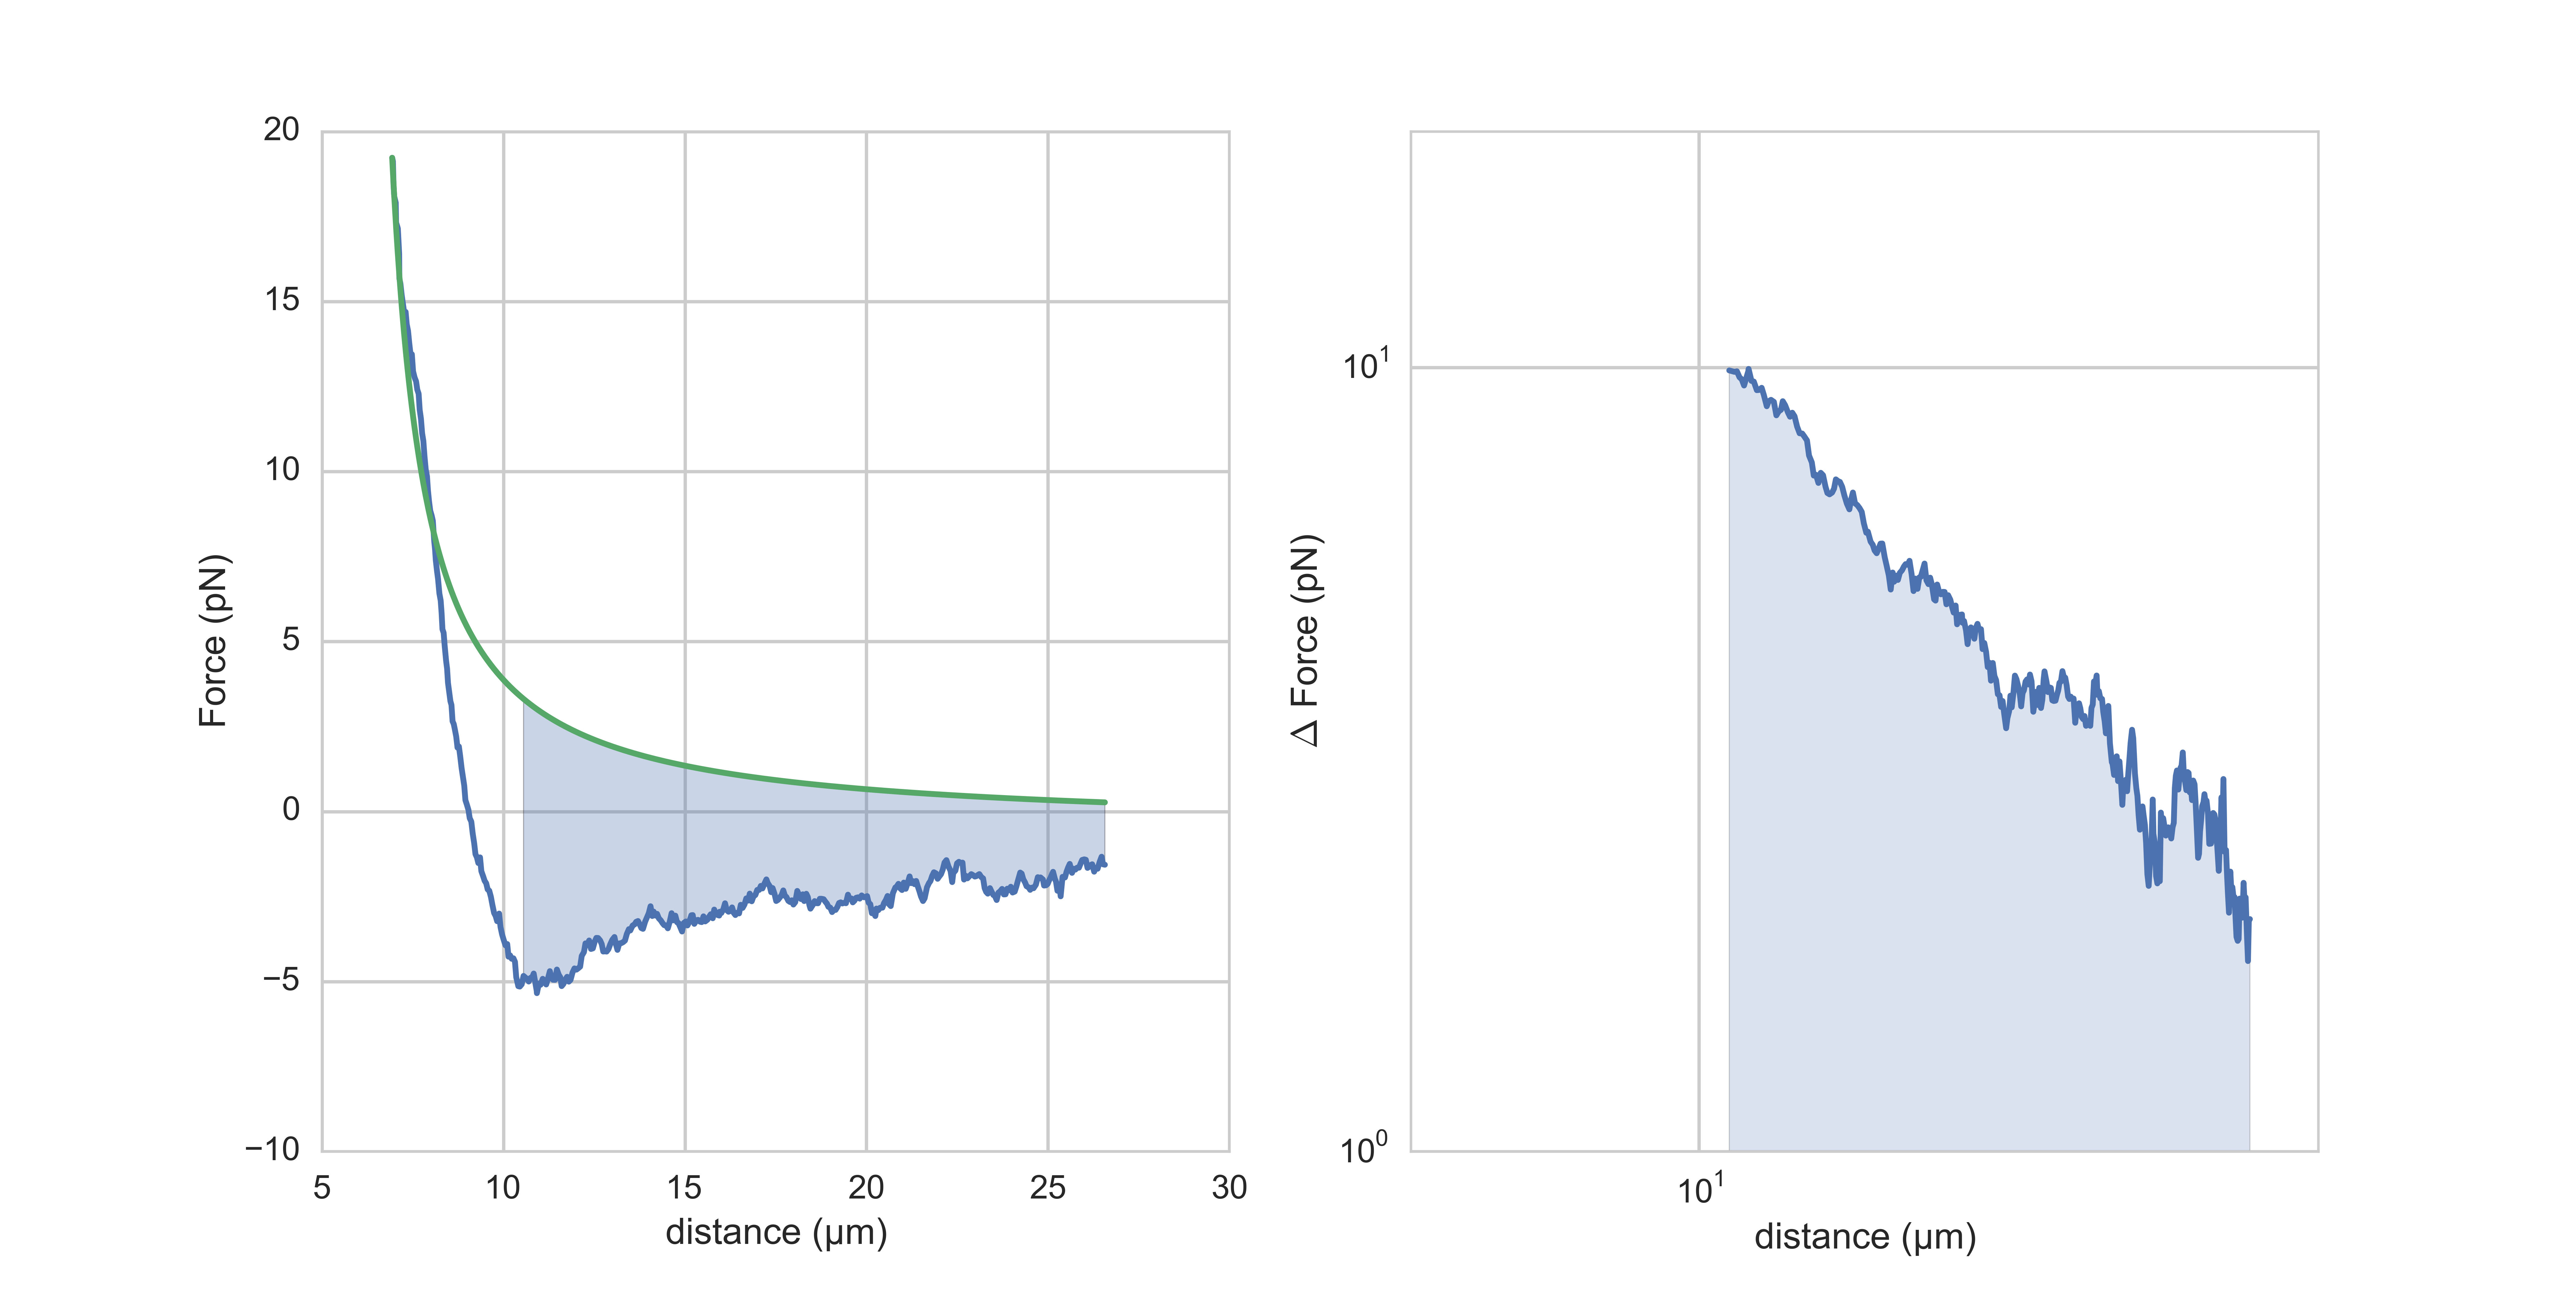
\includegraphics[width=1.000\linewidth]{retract-powerlaw.png}
\caption{Left : Retraction phase with approach phase fit damped by
\(\chi(t_2-t1)\) in green. Blue area under the curve is plotted on a
log-log scale on the right, follow a powerlaw.}\label{index-latex:retract-powerlaw}\end{figure}

\(F_{ret}(d)\) seems though to follow the force felt during the approach phase, damped by \(\chi(t)\) (\(F_{da}\)) for \(d
\simeq{D_{bead}}\) and \(F_{da}+F_{plaw}\) for \(d > 10\mu{}m\).  The
typical size of the bead being \(D_{bead}\) we expect the transition from
one regime to the other to be done on a length scale of \(D_{bead}\) Thus
we use a smoothing function which is a convolution between the projected bead
area and a linear ramp function which can be seen on \hyperref[index-latex:interp]{figure  \ref*{index-latex:interp}}
\begin{figure}[htbp]
\centering
\capstart

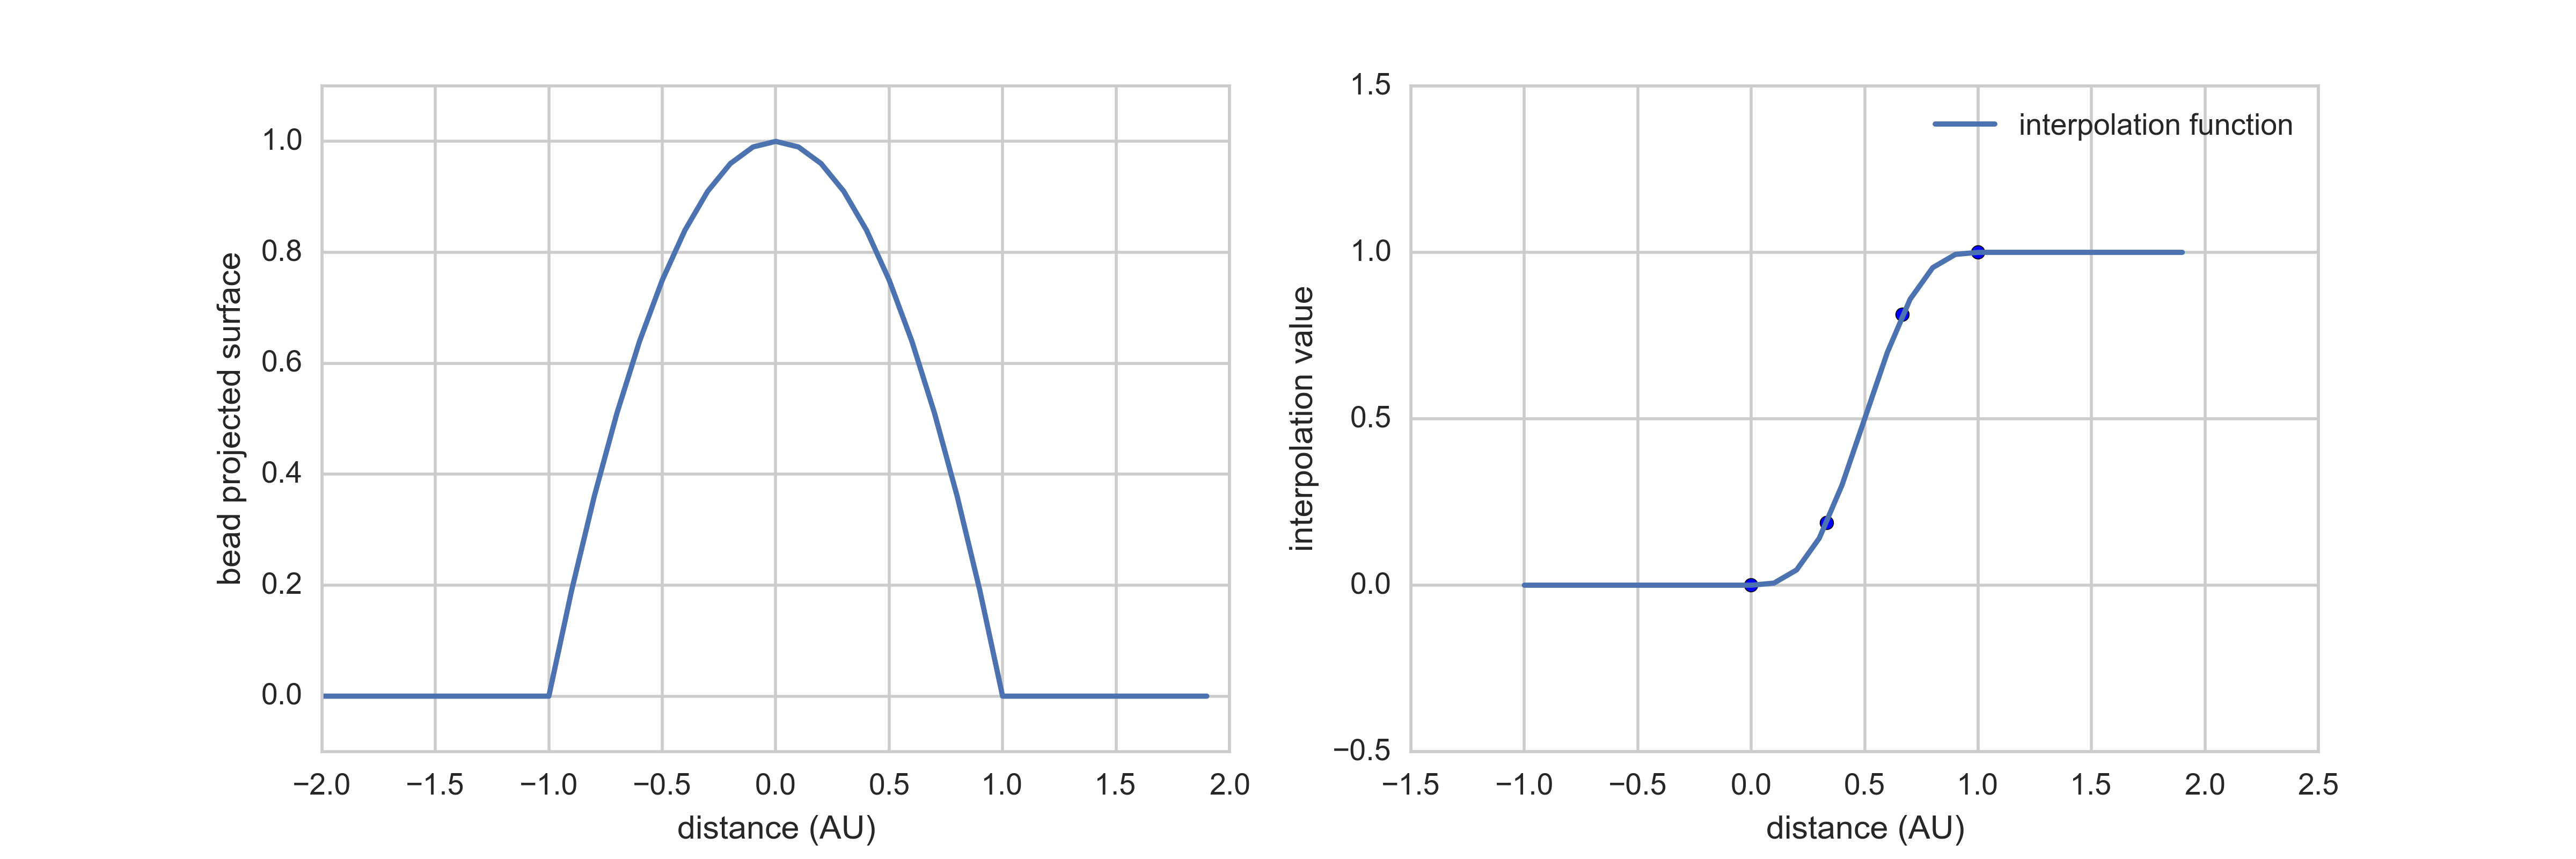
\includegraphics[width=0.900\linewidth]{interpolation.png}
\caption{Interpolation function used to smooth the transition from \(F_{da}\) to
\(F_{da}+F_{plaw}\)}\label{index-latex:interp}\end{figure}

The complete retraction force can be seen on \hyperref[index-latex:fit-3-phases]{figure  \ref*{index-latex:fit-3-phases}} and is equal to
\phantomsection\label{index-latex:equation-eqa314}\begin{gather}
\begin{split}F_{ret}(d) &= F_{da}(d)\times(1-S(d)) + F_{plad}(d)\times S(d)\\\end{split}\label{index-latex-eqa314}
\end{gather}
Where \(S(d)\) is the interpolation function for a bead of 4.34 µm
diameter. We can see that the model represents correctly the retraction and especially
the position and value of the minimum of the retraction function without
fitting parameters when we use the diameter of the probe bead as a typical scale
for the transition when changing direction.


\section{Discussion}
\label{index-latex:discussion}
The actin cytoskeleton plays an important role in many cellular functions.  The
actin cortex, just beneath the cell membrane is not only a crucial structure
for cell motility and the mechanical properties of the cell, it is also an essential
component in cell division and the positioning of the spindle.
Other actin structures, that spawn from the nucleus to the cell membrane are
responsible for cell organelle positioning like in plants where the nucleus is found
towards the anticlinal wall of the cell {\hyperref[index-latex:iwabuchi2010]{{[}Iwabuchi, Takagi,  2010{]}}}, or during
nurse cell maturation where the nucleus is pushed away from the dumping channel:cite:\emph{Huelsmann2013}. The mechanical link from the
outside of the cells to the nucleus using actin bundles has already been show previously
{\hyperref[index-latex:jaalouk2009]{{[}Jaalouk, Lammerding,  2009{]}}}. We show here that these actin structure should not be the
only one taken into account to explain organelles positioning.

Our experiments show the existence of a sparse and stiff actin cloud emanating
from a biomimetically reconstituted actin cortex.  This actin cloud is capable
of staining forces of tens of pico Newtons, enough to hold organelles in place. Using polymer physics
we are able to model the behavior of such an actin cloud and
measure many of its mechanical properties. It provides an
actin scaffold capable of deforming non-plastically. At time scale of few
seconds if behaves mostly elastically with an elastic module of a few Pascal.
The Poisson ratio of the actin cloud varies from 0.1 to 0.2 hinting for a
sparse structure of loosely entangle filaments forming a meshwork with a
typical mesh size of 300 to 400 nm.

The filaments at the origin of this loosely entangled network would emanate from
the dense actin cortex that can be seen and simulated on actin-beads
{\hyperref[index-latex:kawska2012]{{[}Kawska, Carvalho, Manzi,  et al.  2012{]}}} and the evolution of parameters of this actin cloud are
coherent with the preceding studies on biomimetically reconstituted actin
cortices. Recently, the role of actin networks with similar properties as the
actin cloud have been described in cells such as \emph{Xenopus} Oocyte
{\hyperref[index-latex:feric2013]{{[}Feric, Brangwynne,  2013{]}}}. Poisson ratios of actin networks have been
measured in bulk to be higher {\hyperref[index-latex:gardel2003]{{[}Gardel, Valentine, Crocker,  et al.  2003{]}}} but are not inconsistent with our measurement at lower actin concentration.

The actin cloud provides a novel structure that should be studied further to
understand the positioning of organelles in cells and to study which role this sparse
actin structure plays in the formation of other actin networks inside cells.

In particular microrheology experiments could be performed on the growing actin
cloud in order to further characterize the frequency dependence of the mechanical
properties  of the actin cloud. The effect of cross linking and network
branching is crucial for the occurrence of symmetry breaking on bead systems, and
would likely play a role in the structure of the actin cloud. A confined
geometry and direct polymerisation on membrane, or the effect of myosin motors
might allow to alter the properties of the actin cloud.

All these could be cellular mechanisms to use the actin cloud in order
to efficiently form structures needed for its function.
Further studies of the actin cloud on biomimetic or \emph{in vivo} system are
challenging, but would lead to a better understanding of the mechanics of the
cells and its control.

A Paper based on this study has been accepted for publication in Biophysical
Journal and is added for information as appendix of this manuscript.


\chapter{Cortical tension measured on liposome doublets}
\label{index-latex:lib-doub}\label{index-latex:cortical-tension-measured-on-liposome-doublets}\label{index-latex::doc}

\section{Introduction}
\label{index-latex:introduction}
We have seen that in cells the actin cytoskeleton is a key component to form
structures like the actin cortex that serve to transmit forces and gives
mechanical rigidity to cells. In order to drive shape changes, cells regulate the
mechanical properties of the sub-micrometer thick actin cortex that is found
beneath the membrane {\hyperref[index-latex:clark2013]{{[}Clark, Dierkes, Paluch,  2013{]}}}. The dynamics of the actin cortex
drives cell shape changes {\hyperref[index-latex:salbreux2012b]{{[}Salbreux, Charras, Paluch,  2012{]}}} and the presence of the
molecular motor myosin II plays a fundamental role for the tension of the
acto-myosin cortex {\hyperref[index-latex:tinevez2009]{{[}Tinevez, Schulze, Salbreux,  et al.  2009{]}}}. Cortical tension can be measured on
cells to vary between 50 and 4000 pN/µm depending the activity of actin and
myosin.  These changes of the cortical tension are also affected by cell-cell
adhesions {\hyperref[index-latex:maitre2012]{{[}Maitre, Berthoumieux, Krens,  et al.  2012{]}}} which have been shown to play a main role in cell
sorting.

Recently, such acto-myosin cortices have been reconstructed on cell-sized
liposomes {\hyperref[index-latex:carvalho2013a]{{[}Carvalho, Lemiere, Faqir,  et al.  2013{]}}} which showed that the attachment of the actin
cortex to the membrane plays a crucial role in the behavior and contractility
of the acto-myosin network.

In the present study, I collaborated with Kévin Carvalho and Joël Lemière to
further extend the previously developed system {\hyperref[index-latex:carvalho2013a]{{[}Carvalho, Lemiere, Faqir,  et al.  2013{]}}} with the
aim to monitor the cortical tension changes in a biomimetic actin cortex formed
on liposomes. My principal contribution was the analysis of the 3D data that
was acquired using Spinning Disk Microscopy. For the analysis I developed a
novel method to get an precise and unbiased measure of the geometrical
parameter.

To determine the role of cortical tension in cells, recent work used cell
doublets {\hyperref[index-latex:maitre2012]{{[}Maitre, Berthoumieux, Krens,  et al.  2012{]}}}.  Here we form similar doublets from liposomes
around which we polymerize an actin cortex \emph{in vitro} (\hyperref[index-latex:fig1a]{Fig  \ref*{index-latex:fig1a}}). The
shape changes of these liposome doublets allow the time dependent monitoring of
cortical tension in a non-invasive way.  In this project we hence develop a
method for the precise acquisition of doublet deformation in order to determine
accurately the increase of tension induced by the injection of myosin motor on
the preformed actin cortex.


\section{Experimental description}
\label{index-latex:experimental-description}

\subsection{Formation of liposomes doublets}
\label{index-latex:formation-of-liposomes-doublets}
Liposomes are obtain by electro-formation (see {\hyperref[index-latex:electroformation]{\emph{Material and methods}}} (\autopageref*{index-latex:electroformation})) from a mix of EPC and PEG-biotin lipids. The presence of
streptavidin in the working buffer allow liposomes to naturally stick together
to form doublets after 15 minutes (\hyperref[index-latex:fig1a]{Fig  \ref*{index-latex:fig1a}}).
\begin{figure}[htbp]
\centering
\capstart

\includegraphics[width=0.500\linewidth]{Fig_01-A.png}
\caption{Cell-sized liposome doublets. Doublets are indicated by white arrows in
the field of view of a phase contrast microscope.}\label{index-latex:fig1a}\end{figure}


\subsection{Formation of actin cortex on doublets}
\label{index-latex:formation-of-actin-cortex-on-doublets}
Formation of the actin network on doublets is done similar as described
recently {\hyperref[index-latex:carvalho2013a]{{[}Carvalho, Lemiere, Faqir,  et al.  2013{]}}}.  Briefly, actin filaments including
biotinylated monomers are stabilized by phalloidin and linked to PEG-Biotin
lipids (see {\hyperref[index-latex:m-et-m]{\emph{materials and methods}}} (\autopageref*{index-latex:m-et-m}))  via streptavidin that is
present in the solution (\hyperref[index-latex:fig1b]{Fig  \ref*{index-latex:fig1b}}).  Besides linking the actin to the
membrane, it also cross-links the filaments.  Such a network has already been
characterized recently {\hyperref[index-latex:carvalho2013a]{{[}Carvalho, Lemiere, Faqir,  et al.  2013{]}}}.  Note that as the actin filaments
are only added after the formation of the doublets, the interface between the
two liposomes composing the doublets remains free of F-actin (\hyperref[index-latex:fig1c]{Fig  \ref*{index-latex:fig1c}}, \hyperref[index-latex:fds]{ \ref*{index-latex:fds}}). As the actin added is fluorescent, the absence of actin
at the liposome interface can be checked by epifluorescence as it appears dark
compared to the rest of the doublet(\hyperref[index-latex:fig1c]{Fig  \ref*{index-latex:fig1c}}).
\begin{figure}[htbp]
\centering
\capstart

\includegraphics[width=0.700\linewidth]{doublets-schema.png}
\caption{Formation of doublets: 1) In the presence of streptavidin, single liposome
(A) aggregate into doublets. (B) The addition of biotinylated actin
filaments stabilized with phalloidin (2) forms liposome doublets covered
with a micrometer-sized actin network (C). The interface between the two
liposome is a double lipid bilayer free of actin filaments.}\label{index-latex:fds}\end{figure}
\begin{figure}[htbp]
\centering
\capstart

\includegraphics[width=0.500\linewidth]{Fig_01-B.png}
\caption{Schematic of the stabilized actin cortex at the membrane (proteins not to scale).}\label{index-latex:fig1b}\end{figure}


\subsection{Visualisation of the interface}
\label{index-latex:visualisation-of-the-interface}\begin{figure}[htbp]
\centering
\capstart

\includegraphics[width=0.500\linewidth]{Fig_01-C.png}
\caption{i) Flow-chamber designed for buffer exchange. Doublets
are visualized in the middle horizontal channel of the H shape chamber to
avoid movement during the buffer exchange. Spinning disk images of the
doublet before i) or after iii) myosin II injection. One liposome contains the fluorophore
SRB (red) to visualize the interface of the doublet. The actin cortex is
labeled in green. Scale bar 5µm.}\label{index-latex:fig1c}\end{figure}

To visualise the interface between the liposomes, and to avoid the use of fluorescent
lipids that may affect the membrane mechanics {\hyperref[index-latex:sandre1999]{{[}Sandre, Moreaux, BrochardWyart,  1999{]}}} the inside
buffer of approximately half the liposomes are labeled with 0.9 µM
of sulphorhodamin B (SRB)
eventually leading to half of the doublets containing a single fluorescent liposome (\hyperref[index-latex:fig1c]{Fig  \ref*{index-latex:fig1c}} i and iii).


\subsection{Geometrical parameters}
\label{index-latex:geometrical-parameters}
To study the doublet geometry we model each liposome as well as the interface
between them as two spherical caps with their respective center and radius, as
sketched in \hyperref[index-latex:fig-notations-doublets]{figure  \ref*{index-latex:fig-notations-doublets}}.
\begin{figure}[htbp]
\centering
\capstart

\includegraphics[width=0.500\linewidth]{notations-doublets.png}
\caption{Notation of parameters for the doublet model: \(R_1\), \(R_2\), \(R_i\) are respectively the
radius of the liposome 1, the liposome 2 and the interface. \(d\) is the
distance between the liposome centers. \(\theta_1\) and \(\theta_2\) are the angles between
the tangents of the liposome surface and the tangent to the interface at the
contact line. The total contact angle \(\theta\) is the sum of \(\theta_1\) and \(\theta_2\).}\label{index-latex:fig-notations-doublets}\end{figure}

The center position in 3D (X,Y,Z) and the radius (R) of the three spherical caps
completely determine the doublet geometry, though it is interesting to look at other
parameters of the doublets which are :
\begin{itemize}
\item {} 
the total volume of the liposome doublets \emph{V}

\item {} 
the contact angle between the two liposomes

\item {} 
Each of the ``half''-contact angles which are the angle between the
interface and each of the liposomes \(\theta_1,\theta_2\)

\item {} 
The distance between the liposome centers.

\end{itemize}


\section{Experimental Observations}
\label{index-latex:experimental-observations}

\subsection{Effect of myosin-II injection}
\label{index-latex:effect-of-myosin-ii-injection}
We image the liposomes doublets in an open chamber either in phase contrast
and epifluorescence, or spinning disk microscopy in the red (sulphorhodamin)
and green (actin) channel.

Muscle Myosin II that forms {\hyperref[index-latex:myoii]{\emph{bipolars filaments}}} (\autopageref*{index-latex:myoii}) is carefully injected into
the chamber, and leads within minutes to a shape change (\hyperref[index-latex:doublets-contraction]{Fig  \ref*{index-latex:doublets-contraction}})
of the doublets due to the contraction of the actin cortex.
\begin{figure}[htbp]
\centering
\capstart

\includegraphics[width=0.300\linewidth]{doublet-contract.png}
\caption{Doublets contraction showing green channel (actin): (A) doublet before
myosin II injection. (B) doublet during contraction due to myosin II. Time=0 corresponds to myosin II injection.
Scalebar is 5 µm}\label{index-latex:doublets-contraction}\end{figure}

The distance between the liposome centers decreases as the total angle \(\theta
= \theta_1+\theta_2\) increases. The contact angle and other parameters of the
doublets are obtained by fitting spherical caps onto the 2D epifluorescence
images or on the 3D confocal stack as {\hyperref[index-latex:full3dfit]{\emph{described later}}} (\autopageref*{index-latex:full3dfit}).  In the absence of myosin, the
contact angle \(\theta\) is measured to be \(\theta = 64 \pm 16 ^{\circ}\) (n=18) whereas in
the presence of myosin II (200 nM) we find a value of \(\theta = 86 \pm 21
^{\circ}\) (n=5). Measurements of the contact angle after myosin II injection are done before the cortex
ruptures as characterized in {\hyperref[index-latex:carvalho2013a]{{[}Carvalho, Lemiere, Faqir,  et al.  2013{]}}}.


\subsection{Relation between the angles and tension}
\label{index-latex:relation-between-the-angles-and-tension}
Each liposome has its respective tension \(\tau_1\), and \(\tau_2\).  In the absence
of the biomimetic acto-myosin cortex these tensions correspond only to the
tension of the liposome membrane. The interface between the two liposomes is
formed by two lipid bilayers, and the inter-facial tension is composed of two contributions:
The tension of the lipid bilayer, noted \(\tau_i\), and the
adhesion energy per surface unit \(W\) due to the biotin-streptavidin-biotin link
between the two lipid bilayers. The total tension at the interface can thus be
written \(\tau_t = \tau_i -W\) {\hyperref[index-latex:maitre2012]{{[}Maitre, Berthoumieux, Krens,  et al.  2012{]}}}.

As the movement of the contact line during the contraction is slow (order of
µm/min) compared to pressure equilibration across the doublet, we can consider
the contact line between the liposomes and the interface to be at equilibrium.
Hence, we can apply Young's equation:
\phantomsection\label{index-latex:equation-eqa401}\begin{gather}
\begin{split}\sum_{k \in interfaces} \tau_k. \vec t_k  = \vec 0 \\
\tau_i \vec t_i + \tau_1 \vec t_1 + \tau_2 \vec t_2 + = \vec 0\end{split}\label{index-latex-eqa401}
\end{gather}
In which \(t_k\) are the vectors tangent to the interface at the point of
contact, as described in \hyperref[index-latex:fig-yd]{figure  \ref*{index-latex:fig-yd}}
\begin{figure}[htbp]
\centering
\capstart

\includegraphics[width=0.600\linewidth]{yd.png}
\caption{Equilibrium of the contact line. Each interfaces pull on the line with a
force proportional to its tension. As the contact line is at equilibrium
the some of the force compensate which allow to get a relation between the
tensions and the contact angles.}\label{index-latex:fig-yd}\end{figure}

This allows
to relate the tension of each of the lipid layers and the angle
between them at each instance of the contraction. We can in particular project
the result of this equation onto the direction of the contact surface
tangent (dotted line on \hyperref[index-latex:fig-yd]{figure  \ref*{index-latex:fig-yd}}):
\phantomsection\label{index-latex:equation-young-tangent}\begin{gather}
\begin{split}\tau_i - W = \tau_1.cos(\theta_1) + \tau_2.cos(\theta_2)\end{split}\label{index-latex-young-tangent}
\end{gather}
And on the direction perpendicular to it :
\phantomsection\label{index-latex:equation-young-perpendicular}\begin{gather}
\begin{split} \tau_1.sin(\theta_1) = \tau_2.sin(\theta_2)\end{split}\label{index-latex-young-perpendicular}
\end{gather}
These equations link the tension to the contact angle both before, during and
after the contraction and hence remain correct during the experiment. In the following we will mark the values
before the contraction phase by
the suffix \emph{0}. Thus, for example \(\tau_{i,0}\) refers to the
tension of the interface before the addition of myosin, and \(\tau_i\) refers to the
tension of the interface at any instant of the contraction.


\subsection{Contact angle dispersion}
\label{index-latex:contact-angle-dispersion}
The value of the contact angle \(\theta\) varies across different doublets both before
and after the  addition of myosin II. This reflects initial variations of tension in
\(\tau_{i,0}\), \(\tau_{1,0}\), and \(\tau_{2,0}\) from doublet to doublet. Such variations could be
due to a difference in the liposome tension acquired during the different preparations, but also due to a
variation of adhesion energy between doublets, or alternatively an effect of tension build-up
during the formation of the actin shell. As the dispersion in contact angle is
in the same order as the increase in angle upon addition of myosin, a
statistical analysis of the contact angle before and during contraction is
problematic. Thus to avoid this effect of dispersion, we follow the evolution of
\(\theta\) each individual doublet during time.


\subsection{Tension of actin-shell}
\label{index-latex:tension-of-actin-shell}
In order to investigate the increase of tension due to the acto-myosin network
on liposomes, we first characterise the increase that is only due to the addition of the actin-shell in
the absence of myosin. By destroying the F-actin via photo-bleaching (\hyperref[index-latex:fig2a]{Fig  \ref*{index-latex:fig2a}}) we compare the shape of the
same doublets in the presence and absence of the actin-shell. It should be noted that it is established that the
actin filaments are destroyed by bleaching as this process frees oxygen radicals that denature the actin monomers. Hence, the bleaching process
actually destroys the actin cortex ({\hyperref[index-latex:vandergucht2005]{{[}vdGucht, Paluch, Plastino, Sykes,  2005{]}}}).
This investigation showed that the total contact
angle changes by \(3.4 \pm 2.0 ^{\circ}\) (n=7) after disruption (\hyperref[index-latex:fig2b]{Fig  \ref*{index-latex:fig2b}}) of the actin network.
Thus we conclude that the change of tension due of the actin-shell is small and negligible
compared to the change in tension we see with myosin.
\begin{figure}[htbp]
\centering
\capstart

\includegraphics[width=0.500\linewidth]{Fig_02-A.png}
\caption{Image of an individual doublet coated with fluorescent F-actin before i) ii) and
after iii) iv) actin cortex disruption. The actin cortex is visualized by
epifluorescence ii) iv) and the doublet by phase contrast i) iii). Scale
bar 5µm.}\label{index-latex:fig2a}\end{figure}
\begin{figure}[htbp]
\centering
\capstart

\includegraphics[width=0.500\linewidth]{Fig_02-B.png}
\caption{Measurement of the contact angle between the two liposomes forming the
doublet before (black) and after (white) disruption of the stabilized actin
cortex as a function of their volume.}\label{index-latex:fig2b}\end{figure}


\section{3D observation}
\label{index-latex:d-observation}\label{index-latex:d-obs}
Three dimensional imaging of the doublets is necessary to get the correct
contact angle. This requirement comes from the fact that in simple 2D epifluorescence
images, the focal plane would have to correspond to the equatorial plane of the doubles for correct analysis. If
this is not the case, the fit will produce a systematic underestimation of the contact angle.
This is especially the case when doublets are of different radii as typically found in our
experiments, where the liposomes composing the doublets have an ratio of \(R_1 / R_2\) between 1.15 and 1.82.
\begin{figure}[htbp]
\centering
\capstart

\includegraphics[width=0.900\linewidth]{light_table.png}
\caption{Confocal stack of an liposome doublet actin channel, 3D reconstruction in
\hyperref[index-latex:fig3a]{figure  \ref*{index-latex:fig3a}}. Note that there is no actin at the interface between
the liposomes (Frames \#11-\#14). The distance between each image is \(\Delta z=0.85\) µm.}\label{index-latex:confocal-stack}\end{figure}
\begin{figure}[htbp]
\centering
\capstart

\includegraphics[width=0.500\linewidth]{Fig_03-A.png}
\caption{3D reconstruction of a doublet surrounded by actin. The absence of actin on
the interface can be seen more easily on \hyperref[index-latex:confocal-stack]{figure  \ref*{index-latex:confocal-stack}}.}\label{index-latex:fig3a}\end{figure}

Time resolved 3D Spinning disk stacks (\hyperref[index-latex:confocal-stack]{Fig  \ref*{index-latex:confocal-stack}} with 3D reconstruction
\hyperref[index-latex:fig3a]{Fig  \ref*{index-latex:fig3a}}) are recorded with a time resolution of less than 5 seconds per stack for an accurate determination of the different
parameters of the doublet over time. The analysis reveals the contact angle \(\theta\) (\hyperref[index-latex:fig3b]{Fig  \ref*{index-latex:fig3b}}) , the
volume of the doublet \(V\) (\hyperref[index-latex:fig3d]{Fig  \ref*{index-latex:fig3d}}) and the distance between liposome
centers \(d\) (\hyperref[index-latex:fig3c]{Fig  \ref*{index-latex:fig3c}}). All theses parameters are obtain by
fitting spherical 3D caps on the 3D stack as explained {\hyperref[index-latex:full3dfit]{\emph{later}}} (\autopageref*{index-latex:full3dfit}).
\begin{figure}[htbp]
\centering
\capstart

\includegraphics[width=0.500\linewidth]{Fig_03-B.png}
\caption{Evolution of the contact angle compared to its initial value as a function of
time.  Each doublet is represented by a different colors. The color code corresponds to the doublet
shown in figure \hyperref[index-latex:fig3c]{ \ref*{index-latex:fig3c}}, \hyperref[index-latex:fig3d]{ \ref*{index-latex:fig3d}}
and \hyperref[index-latex:fig3e]{ \ref*{index-latex:fig3e}}. A special case is shown in the blue dashed line,
where the actin cortex on the doublet ruptured, and the cortex is peeled off.
The analysis of this case showed that the contact angle after rupture recovers its initial value.}\label{index-latex:fig3b}\end{figure}
\begin{figure}[htbp]
\centering
\capstart

\includegraphics[width=0.500\linewidth]{Fig_03-C.png}
\caption{Evolution of the distance between liposome centers as a function of time.
Same color code for same doublets as in figure \hyperref[index-latex:fig3b]{ \ref*{index-latex:fig3b}}, \hyperref[index-latex:fig3d]{ \ref*{index-latex:fig3d}}
and \hyperref[index-latex:fig3e]{ \ref*{index-latex:fig3e}}. Again the doublet with the ruptured cortex recovers its initial parameter values.}\label{index-latex:fig3c}\end{figure}
\begin{figure}[htbp]
\centering
\capstart

\includegraphics[width=0.500\linewidth]{Fig_03-D.png}
\caption{Evolution of the volume ratio over time.
Same color code for same doublets as in figure \hyperref[index-latex:fig3b]{ \ref*{index-latex:fig3b}}, \hyperref[index-latex:fig3c]{ \ref*{index-latex:fig3c}}
and \hyperref[index-latex:fig3e]{ \ref*{index-latex:fig3e}}.}\label{index-latex:fig3d}\end{figure}

During contraction triggered by myosin, we observe that the contact angle
\(\theta\) increases while the distance between liposome centers \(d\) decreases.
During this process the volume remains constant within the error of 10\%.  These
results are consistent with the measure of contact angle in freely adhering cell
doublet experiments done previously {\hyperref[index-latex:maitre2012]{{[}Maitre, Berthoumieux, Krens,  et al.  2012{]}}}.


\section{Discussion}
\label{index-latex:discussion}

\subsection{Cortical tension is homogeneous for single doublet}
\label{index-latex:cortical-tension-is-homogeneous-for-single-doublet}
Combining equation \eqref{index-latex-young-perpendicular} with the finding that \(\theta_1 = \theta_2 = \theta
/2\) allows to infer the equality of tension on both side of the doublet during all the
experiments. We can hence write \(\tau_1 = \tau_2 = \tau\). This result is
consistent with the fact that actin is distributed continuously all around the
liposome doublet. Hence, myosin II minifilaments pull on a continuous shell. In
these conditions equation \eqref{index-latex-young-tangent} simplifies to :
\phantomsection\label{index-latex:equation-eq3}\begin{gather}
\begin{split}\tau_i - W = 2.\tau(t).cos(\theta(t)/2)\end{split}\label{index-latex-eq3}
\end{gather}
Where \(\tau(t)\) and \(\theta(t)\) are the tension and the angle at
the time t after myosin injection. Assuming that
\(\tau_i-W\) may depend on a variability of the initial adhesion between
liposomes. Since myosin does not operate at the interface between liposome as
this is free from actin, it is reasonable to consider the tension and
adhesion energy constant for a given doublets over time
\(\tau_i-W = \tau_{i,0}-W_0\).
Therefore we obtain an expression of the tension \(\tau(t)\) during the acto myosin contraction that reads :
\phantomsection\label{index-latex:equation-eqtime}\begin{gather}
\begin{split}\tau(t) &= \frac{ \tau_i - W }{2.cos(\theta/2)}\\
        &= \frac{ cst           }{2.cos(\theta/2)}\end{split}\label{index-latex-eqtime}
\end{gather}
Hence we can evaluate the tension relative to its initial value over time :
\phantomsection\label{index-latex:equation-eqa402a}\begin{gather}
\begin{split}\frac{ \tau(t) }{\tau_0} = \frac{cos(\theta_0/2)}{cos(\theta(t)/2)}\end{split}\label{index-latex-eqa402a}
\end{gather}

\subsection{Relative increase in cortical tension}
\label{index-latex:relative-increase-in-cortical-tension}
Interaction of myosin II filaments with a biomimetic actin cortex induces
tension build up. The cortical tension, normalized to its initial value,
increases and reaches a plateau where \(\tau(t) = \tau_{peeling}\)
(\hyperref[index-latex:fig3e]{Fig  \ref*{index-latex:fig3e}}) with the same trend as \(\theta\).  Note that if the acto-myosin shell
breaks and peels, the doublet recovers its initial shape (see dashed blue line
for \(d\) and \(\theta\) on  \hyperref[index-latex:fig3b]{Fig  \ref*{index-latex:fig3b}}, \hyperref[index-latex:fig3c]{ \ref*{index-latex:fig3c}}, \hyperref[index-latex:fig3d]{ \ref*{index-latex:fig3d}} ). The average relative tension is found to
be \(\tau_{peeling}/\tau_0 = 1.56 \pm 0.56\) (n=5) in 3D and
\(\tau_{peeling}/\tau_0  = 1.25 \pm 0.15\) (n=5) in epifluorescence, in
agreement with discussed expected underestimation of the contact angle in epifluorescence measurements.
\begin{figure}[htbp]
\centering
\capstart

\includegraphics[width=0.500\linewidth]{Fig_03-E.png}
\caption{Increase of the tension ratio between the tension \(\tau(t)\) at time
\(t\) and the initial one \(\tau_0\).
Same color code for same doublets as in figure \hyperref[index-latex:fig3b]{ \ref*{index-latex:fig3b}}, \hyperref[index-latex:fig3c]{ \ref*{index-latex:fig3c}}
and \hyperref[index-latex:fig3d]{ \ref*{index-latex:fig3d}}. The actin cortex rupture in the blue dashed line also presents the highest relative tension increase.}\label{index-latex:fig3e}\end{figure}


\subsection{Cortical tension increase in doublets and in cells}
\label{index-latex:cortical-tension-increase-in-doublets-and-in-cells}
In cells, cortical tension can be as low as 50 pN/µm in fibroblast progenitor
cells {\hyperref[index-latex:krieg2008]{{[}Krieg, ArboledaEstudillo, Puech,  et al.  2008{]}}} and can go up to 4000 pN/µm for
dictyostelium {\hyperref[index-latex:schwarz2000]{{[}Schwarz, Neuhaus, Kistler,  et al.  2000{]}}}. Surprisingly, when myosin activity is
affected, either by drugs or by genetic manipulation, the cortical tension only
decreases by a factor of about 2. Cells are also observed to round up during
division  in which an  increase of tension by a factor of two
is sufficient {\hyperref[index-latex:stewart2011]{{[}Stewart, Helenius, Toyoda,  et al.  2011{]}}}, {\hyperref[index-latex:kunda2008]{{[}Kunda, Pelling, Liu, Baum,  2008{]}}} .
Our \emph{in vitro} reconstruction is able to reproduce similar
changes of cortical tension as we observe a cortical tension increase by a factor of up to 2.4.


\subsection{Different contributions for cortical tension}
\label{index-latex:different-contributions-for-cortical-tension}
Cortical tension is the sum of the membrane tension and the tension due to the
acto myosin cortex. We question how the membrane contributes to cortical tension
and in our assay we show that it may account for approximately 50\% of the cortical tension in some cases.
In suspended fibroblast cells, membrane tension is estimated to be 10\% of the
cortical tension {\hyperref[index-latex:tinevez2009]{{[}Tinevez, Schulze, Salbreux,  et al.  2009{]}}}. When polymerisation of actin is
stimulated, the cortical tension is multiplied by a factor of 5 showing a
strong dependence also with actin dynamics {\hyperref[index-latex:tinevez2009]{{[}Tinevez, Schulze, Salbreux,  et al.  2009{]}}}. Hence he
residual tension in cells might be due to actin dynamics which is absent in our
experiments. How actin contribute to cortical tension is still an open question
that needs to be addressed in the cell geometry.  Whereas actin polymerisation
outside a liposome has been shown to generate inward pressure,
how this can be translated to tension  in a different geometry is
not yet clear. \emph{In vitro} assays are on their way to mimic actin dynamics in
cells {\hyperref[index-latex:abushah2014]{{[}AbuShah, Keren,  2014{]}}} and will allow to unveil the mechanisms of tension build up by
actin dynamics, which is the remaining module that needs to be understood. The
effect of myosin and of the membrane being clarified in this study.


\subsection{Conclusion}
\label{index-latex:conclusion}
We provide a biomimetic reconstitution of the tension build up by acto-myosin
contractility using liposome doublets. Cortical tension changes are visualized
\emph{in situ} over time by analyzing doublet shape changes. This method allows us
to directly quantify the relative increase in tension due to myosin, separately
from the one due to actin dynamics. Understanding the contraction of composite systems
that are rebuilt brick by brick to finally model a living cell will hopefully lead the way towards for a reconstitution
of complex systems like tissues.


\section{3D fitting}
\label{index-latex:full3dfit}\label{index-latex:d-fitting}
Obtaining the geometrical parameter of doublets remains challenging as in
classical phase contrast and epifluorescence microscopy the acquired images
only capture a single focal plane of the doublets. This makes the analysis
difficult as the observation plane should be the
equatorial plane of the doublet.

In order to achieve good precision in the measurements of the contact angle we
decided to use confocal microscopy and acquire evenly spaced z-stacks. From
theses stacks the 3D structure of a doublet was reconstituted. Using the 3D
structure of the doublets allows to recover the geometrical parameters and
the contact angle.

To determine the geometrical parameters of the doublets
we modeled the doublets as two intersecting spheres, determined the expected 3D
images and adjusted the parameters of the model to resemble the obtained
experimental data.

I was responsible for developing a fast and precise method to reliably and
automatically recover the geometrical parameters of the liposome doublets
based in the image stacks acquired using spinning disk microscopy. In the following part I will develop the principle of this
method and the result on liposomes doublets.


\subsection{First step: Fitting a single liposome}
\label{index-latex:first-step-fitting-a-single-liposome}
In this part we show the principle that allow us to determine the 8
geometrical parameter that characterise a doublet: 2 centers (X,Y,Z) and 2 radii
(\(R_1\) and \(R_2\)).

As the principle for finding the geometrical parameter does not differ with the
number of dimensions, the presented methods can be applied even in higher dimensions (e.g. deformed
ellipsoid liposome, or multi channel imaging). Furthermore, the principles remain the same also in a
space with less dimensions, so we will restrict our discussion to a single liposome
in a 2D plane (X,Y position of centers and R, radius) hence reducing the parameters to be determined to six instead of eight.

Experimentally, liposomes are observed using fluorescently labeled actin that
forms an homogeneous micrometer sized actin shell. In the observation plane,
the liposome is a bright ring of given thickness (we will refer to this as the
\emph{expected signal}) , on top of this image is the experimental noise where the
principal noise sources are identified to be the presence of fluorescent actin monomers in the
buffer solution and electronic noise from the CCD camera. Eventually, the noise
in the outside buffer due to monomeric actin can be higher than inside which is
free of actin.

The signal from a liposome and the addition of noise can be replicated
numerically as seen on  \hyperref[index-latex:fig-2d-sim]{figure  \ref*{index-latex:fig-2d-sim}}.
\begin{figure}[htbp]
\centering
\capstart

\includegraphics{modl-2D-doublet.png}
\caption{Left : A simulation of liposome fluorescent image consisting of an uniform shell or membrane
(\emph{expected signal}).  Middle: Same Image Adding Gaussian noise. This simulates
one plane of a confocal Z-stack.  Right: Simulation of liposome with
fluorescently labeled actin shell in a fluorescent external buffer and non
fluorescent inside buffer.}\label{index-latex:fig-2d-sim}\end{figure}

The \emph{expected signal} can be modeled numerically using several parameters of
the system (center and radius of liposome, point spread function of microscope,
...).

To find the correct parameters for the doublets we will numerically correlate
the acquired data with the numerical model and search for the correlation
that correspond best to the real image. The correlation between the model and the images
data can be written.
\phantomsection\label{index-latex:equation-eqa402}\begin{gather}
\begin{split}r_{xy}=\frac{\sum\limits_{i=1}^n (x_i-\bar{x})(y_i-\bar{y})}{(n-1) s_x s_y}\end{split}\label{index-latex-eqa402}
\end{gather}
In which \(x_i\) are luminosity values of each of the \(n\) pixels in
the acquired data, \(y_i\) are the luminosity of the pixels in the model
\(\bar{x},\bar{y}\) correspond to average values over the images,
\(s_x\) and \(s_y\) are the standard deviation of the luminosity
values.

As the monomeric fluorescently labeled actin and the electronic noise are dominant
in the acquired images, we can assume a uniform noise on top of the \emph{expected signal}. The correlation between the model and the noise is in average
uniform.
\phantomsection\label{index-latex:equation-eqa403}\begin{gather}
\begin{split}r_{noise,model(params)} = cst\end{split}\label{index-latex-eqa403}
\end{gather}
And the correlation between the \emph{expected signal} and the model is expected to be
maximal for the parameters of the model that  equal the real geometrical
parameters of the doublets.
\phantomsection\label{index-latex:equation-eqa404}\begin{gather}
\begin{split}{arg\,max}_p\left(r_{data,model(p)}\right)= {arg\,max}_p \left(r_{expectedSignal,model(p)}\right)\end{split}\label{index-latex-eqa404}
\end{gather}
In which \({arg\,max}_p\) stands for the
argument of the maximum, that is to say, the set of points of the given
argument for which the given function reaches its maximum value. Thus searching
for parameter values that maximize the correlation between the model and
the data implies finding the geometrical parameters we are interested in.

We can test the ability to do this numerically by generating data, adding noise
to it and trying to recover the parameters of the \emph{expected signal}.

By looking at the value of the correlation between the generated data and the model
as a function of model parameters, we can check that the correlation
values are maximal when the model center value correspond to the \emph{expected signal}
center value (Fig \ref{index-latex:corr-fun-1}), and when the radius of the model liposome
has the same radius in the model correspond to the radius in the generated data (Fig \ref{index-latex:corr-fun-2}).
\begin{figure}[htbp]
\centering
\capstart

\includegraphics[width=0.500\linewidth]{double-c-_100-by-100-rc-40_0-noise-0_5-delta-4_0_.png}
\caption{Value of the correlation as a function (arbitrary units) of two of the fit
parameters. The radius of the liposome in the model is taken as
equal to the value of the \emph{expected signal}, and the position of the center is
varied in the X and Y direction. The value of the correlation is maximal for
the position of the center in the model that equals the center of the \emph{expected signal}.  We
can see local maxima on the 3D representation that are well below the value
of the global maximum. The peak at the global maxima is sharp, hinting that
the search of the maxima need relatively good initial
parameters (lower than \textasciitilde{}1/10 of liposome radius). The sharpness of the peak
point that corresponds to the best fit parameters on experimental data should be
robust.}\label{index-latex:corr-fun-1}\end{figure}
\begin{figure}[htbp]
\centering
\capstart

\includegraphics[width=0.600\linewidth]{c-R-_100-by-100-RC-40_0-noise-0_5-delta-4_0_.png}
\caption{Same as \hyperref[index-latex:corr-fun-1]{figure  \ref*{index-latex:corr-fun-1}}  with Y position of the center taken
as equal to the expected signal, variating X position of the model and
radius of the liposome. The graph shows the same properties as before.}\label{index-latex:corr-fun-2}\end{figure}

Using minimisation techniques we can search the parameter space of the model and
maximise the correlation between the model and the experimental data. We then
recover the geometrical parameters of the liposomes. This can be done by
efficiently computing the value of the correlation within a few hundreds of
points and which gives access to the liposomes' geometrical parameters, here position
and radius.


\subsection{Fitting a doublet}
\label{index-latex:fitting-a-doublet}
The determination of the contact angle on epifluorescence images or phase contrast
images often results in an underestimation as the imaging plane is not necessarily one of the doublets
equatorial planes. Moreover, most determination of the contact angle on phase
contrast and epifluorescence images are done manually {\hyperref[index-latex:maitre2012]{{[}Maitre, Berthoumieux, Krens,  et al.  2012{]}}} and
are subject to experimenter bias as the experimenter draws the tangent lines at the
contact point between the liposomes. Thus we decided to develop fitting routines for the acquired
3D confocal stacks. In our case we avoid the usage of
fluorescent lipids that could artificially change the tension of the membrane.

As sketched in \hyperref[index-latex:fds]{figure  \ref*{index-latex:fds}}, the doublets are covered with a
thin micrometer-thick layer of fluorescent actin filaments, which we
image by confocal spinning disk microscopy. As the actin-layer is attached to the membrane
and the contact angle is defined as the angle between the lipid bilayer, imaging the actin-layer corresponds
to the angle between the inner surfaces of the two actin networks present on each liposome.

Thus in order to determine the geometrical parameters of the doublets we need
to also model the actin shell. As the liposomes in contact are two spherical
caps the uniform actin layer will also form two spherical caps with a given
thickness. The total image is thus the union of two spherical caps blurred by
the point spread function of the microscope. This can be seen on \hyperref[index-latex:mproj1]{figure  \ref*{index-latex:mproj1}}.  We can see on this image that the doublet is here lying on the
chamber surface. We checked in this case that the contact surface between the
chamber and the doublet did not change during experiments.
\begin{figure}[htbp]
\centering
\capstart

\includegraphics[width=0.800\linewidth]{max_proj_340A.png}
\caption{Maximum projection along X,Y and Z of recorded stacks, green channel represents actin.
One can see that the liposome doublets are lying on the surface of the
observation chamber (arrows).}\label{index-latex:mproj1}\end{figure}

As the contraction of the doublets is rapid, and the recorded 3D stacks contain a
large number of frames. Hence it is crucial to be able to compute the model and the
correlation in a reasonable time (less than an hour per images). To
achieve this besides calculating the model as efficiently as possible one can
replace the exact calculation of two spherical cap and the point spread
function of the microscope by the union and subtraction of pre calculated spheres followed by a 3D
numerical Gaussian blur (\hyperref[index-latex:fig-mdl]{Fig  \ref*{index-latex:fig-mdl}}).
\begin{figure}[htbp]
\centering
\capstart

\includegraphics[width=0.600\linewidth]{3dblur.png}
\caption{Principe of numerically approximating the two spherical caps as intersection of two spheres,
followed by a 3D numerical Gaussian blur. The
numerical speed-up compared to the exact calculation of the fluorescent density allows
to make fits on doublets in minutes instead of hours.}\label{index-latex:fig-mdl}\end{figure}

However, the use of such numerical techniques is not without artifacts.  In the case of
discreet Z-stack that are not sufficiently spaced, the different radii in the
fluorescent rings within subsequent stacks can lead to a ``ring-artifact'' (\hyperref[index-latex:ring-artifact]{Fig  \ref*{index-latex:ring-artifact}}) when using numerical Gaussian blur. In the case of a too
pronounced ``ring-artifact'' a ``ghost'' spheres can appear around each liposome
which can cause the fitting process of the doublets to fall into a local
maximum of correlation, thus leading to wrong value of the geometrical
parameters.
\begin{figure}[htbp]
\centering
\capstart

\includegraphics[width=0.700\linewidth]{ring_artifact.png}
\caption{Left : One plane of the numerical model with an exaggerated ring artifact due
to an under sampling of the model in the Z-direction, stacks from ``Far'' Z
leak onto the current Z-plane and form a ring.  Right : Same plane of the
model with enough sampling plane in the Z-direction do not show the ring
artifact. In this case we use a sampling equal to the number of slice than
the recorded data. (X,Y in arbitrary units)}\label{index-latex:ring-artifact}\end{figure}

In our case we have a sufficient number of planes per stack so that the numerical model
with the same sample size as the data do not show the ring artefact and have
smooth transition near the position of the spherical cap. Though the ring
artifact can be eliminated by oversampling/interpolating the model before the
numerical Gaussian blur and under sampling afterwards to arrive at the correct number of
pixels.

The size of the
Gaussian blur can also be adjusted to be higher which will act as a regularisation
function for the value of the correlation between the model and the acquired
data (see \hyperref[index-latex:max-proj-model]{Fig  \ref*{index-latex:max-proj-model}}), thus smoothing or eliminating local maxima,
but reducing the precision in the position of the maxima.
\begin{figure}[htbp]
\centering
\capstart

\includegraphics[width=0.500\linewidth]{max_proj_model.png}
\caption{Maximum projection along X,Y and Z of numerical model, the ``ring'' effect
can still slightly be seen near the pole of each liposome, but is not
sufficient for the fit to be stuck in a local minimum.}\label{index-latex:max-proj-model}\end{figure}

The value of the correlation between the model and the experimentally recorded
data can be maximised using already available functions, in particular we used
the Nelder–Mead simplex algorithm as implemented in \emph{scipy.optimise} python library. This
gives us the 8 parameters of the doublets. Result of the fits are show in
\hyperref[index-latex:fig-fit-t0]{figure  \ref*{index-latex:fig-fit-t0}}.
\begin{figure}[htbp]
\centering
\capstart

\includegraphics[width=0.500\linewidth]{Doublet-402-A-Fit-t-0.png}
\caption{Maximum projection of confocal images in the X,Y and Z projection as well
as the result of the fits shown as equatorial circles for the three
direction of projection.}\label{index-latex:fig-fit-t0}\end{figure}

Using the fast Cython code ({\hyperref[index-latex:seljebotn2009]{{[}Seljebotn,  2009{]}}}) also allowed to also speed
up fitting to a reasonable time: one Z-stack of 3 millions pixels can be fitted
in about 40 seconds. Thus allowing the fitting of a full 3D movie of a doublets
contraction to be done in less than an hour for 30 to 40 frames.

To ensure robustness of the fits to doublet center displacement during
acquisition, the initial parameter of the fit where chosen manually for each
first frame of each sequences. The final fit parameters of each frame are reused
as initial fit parameter for the subsequent frame.

In order to test robustness of the fit, the initial fit parameters where randomly
modified by an amount of +/- 1µm, and we checked that the final parameters did
not vary.

For a couple of parameters, the values of the correlation function can be plotted
to check for the regularity of the function and the absence of local maxima. \hyperref[index-latex:gof2d]{Figure  \ref*{index-latex:gof2d}} and \hyperref[index-latex:gof3d]{figure  \ref*{index-latex:gof3d}} show the resulting correlation values.
\begin{figure}[htbp]
\centering
\capstart

\includegraphics[width=0.600\linewidth]{gof-2d-doublets.png}
\caption{Correlation of the model and the data as a function of the center position
of one of the model spherical caps along the X axis and the radius of this
same spherical cap. Vertical axis in arbitrary unit.}\label{index-latex:gof2d}\end{figure}
\begin{figure}[htbp]
\centering
\capstart

\includegraphics[width=0.600\linewidth]{gof-3d-doublets.png}
\caption{3D representation of the data in \hyperref[index-latex:gof2d]{figure  \ref*{index-latex:gof2d}}, the shape of the
function is the same as the simulation done with the \emph{expected signal} in
\hyperref[index-latex:corr-fun-1]{figure  \ref*{index-latex:corr-fun-1}} \hyperref[index-latex:corr-fun-2]{and  \ref*{index-latex:corr-fun-2}}}\label{index-latex:gof3d}\end{figure}

The correctness of the fit is also checked visually to prevent errors in the
procedure.  The fit was found to be alway accurate and coherent with manual
measurements of the contact angle.  When the red channel was also present and liposomes
contained sulphorhodamin B, fits where additionally visually checked by using maximum
projection of the red channel.  (see \hyperref[index-latex:srhod]{Fig  \ref*{index-latex:srhod}}).
\begin{figure}[htbp]
\centering
\capstart

\includegraphics[width=0.800\linewidth]{srhod_superimpose.png}
\caption{Maximum projection of the red channel (\emph{sulphorhodamin}) and the fitted
parameter for the doublet.}\label{index-latex:srhod}\end{figure}


\subsection{Discussion}
\label{index-latex:id24}
In this part we show that by modeling the liposome doublet and using
fluorescently labeled actin we are able to develop a technique that
automatically and robustly determine the geometrical properties of the liposome
doublets.

We note that the red fluorescent dye present in the inside buffer of the
liposome could be used conjointly to the green channel in order to improve the
quality of the fit, though this would require the extra parameters of the
interface radius. As the computation time needed to fit the doublets increase
rapidly with the number of parameter, this solution was found to be
impractical.  Moreover, the curvature of the interface being relatively small
and the difference between the curved interface and a flat plane being close to
the optical resolution, hence the fits risk to become unstable.  The use of
fluorescently labeled lipids for the liposome membrane also suffers from the
same issues of extra parameter if one want to recover the position of the
interface.


\subsection{Conclusion}
\label{index-latex:id25}
We developed a robust and automated method to determine the geometrical
parameters of liposome doublets. This allows to determine robustly the
geometrical parameters of liposome doublets without
experimenter measurement bias due to the selection of the illumination plane,
resolution of optics and luminosity scale.

We have seen that liposome doublets with reconstituted acto-myosin cortices are
a biomimetic system that allows to measure the changes in cortical tension with
time. 3D fitting helped to quantify the tension by obtaining the corresponding contact angles.

Observing the contraction of multiple liposomes doublets simultaneously and the
ability to automatically determine the geometrical parameters allows more
sample to be collected. Faster and more reliable data acquisition on actin
network contractions will allow for a better understanding of the effect of actin
network \emph{in vitro} which also pave the way to reconstitution of more complex system.


\chapter{Active cytoplasm movement in mouse oocytes}
\label{index-latex:active-cytoplasm-movement-in-mouse-oocytes}\label{index-latex::doc}

\section{Introduction}
\label{index-latex:introduction}
Mouse oocyte are big spherical cells with a diameter of about 80 µm.  Previous work has shown
that the spindle positioning during meiotic cell division in oocytes depends
on an actin meshwork that is present in the cell's cytoplasm {\hyperref[index-latex:schuh2008]{{[}Schuh, Ellenberg,  2008{]}}}.  This
actin meshwork is regulated by formin that is localized to endogenous vesicles.
Additionally, these vesicles recruit the myosin-Vb motor protein, that are know do drive the active movement
of the vesicles in the cytoplasm {\hyperref[index-latex:holubcova2013]{{[}Holubcova, Howard, Schuh,  2013{]}}}. In a collaborative project with the group of Marie-Hélène Verlhac
and her Postdoc Maria Almonacid at the Collège de France, I designed a way to measure
cytoplasmic activity in mouse oocyte.

In \hyperref[index-latex:oocytewt]{figure  \ref*{index-latex:oocytewt}} a typical mouse
oocyte is presented where the nucleus can be seen to be positioned at the center of the cell.
Current questions in this system relate to the mechanical processes during meiosis such as the chromosome migration,
the asymmetric cell division and the positioning of organelles by the dynamic remodelling of the actin network.
While our team did active and passive microrheology measurements on the timescales or 10 seconds, I developed a
method that is suitable for longer timescales in the order of minutes, that are more relevant for the process of meiosis.
\begin{figure}[htbp]
\centering
\capstart

\includegraphics[width=0.600\linewidth]{oocyte-wild-type.png}
\caption{Bright field image of a mouse oocyte before meiosis (scale bar is 20 µm).
The cell diameter is about 80µm. The nucleus is positioned at the center of
the oocyte during meiosis I by the help of the actin network. The
positioning is a crucial factor for the normal division of the oocyte. The
oocytes are a good reference system as they provide a clean spherical
symmetry and due to their size give a good spatial differences between the
cortex and the cytosol which helps in measuring spatial variations of
mechanical properties and vesicle movement.  Image Credit to Maria
Almonacid, Collège de France.}\label{index-latex:oocytewt}\end{figure}


\section{Oocytes}
\label{index-latex:oocytes}
The cytosolic actin meshwork in oocytes is controlled by the activity of formins (Fmn2) that
nucleate actin polymerisation and by the activity of the vesicle bound molecular motor protein myosin Vb that
controls the dynamic movement of the
vesicles in the actin meshwork. Hence it is of interest to study oocytes that have formin and myosin Vb deficits.
In particular, we focused on three types: 1) Wild types oocyte, 2) oocytes prepared from Formin 2 invalidated female
(Fnm2-/-) that lack the
actin meshwork and 3) oocytes injected with the RNA coding for the dominant-negative tail of Myosin
Vb (\hyperref[index-latex:fig3oo]{Fig  \ref*{index-latex:fig3oo}}), thus replacing the active myosin Vb on the vesicles.
\begin{figure}[htbp]
\centering
\capstart

\includegraphics[width=1.000\linewidth]{3-oocytes.png}
\caption{Bright field image microscopy of the 3 kinds of oocytes (Credit to Maria
Almonacid, Collège de France). WT) Image of Wild Type Oocyte, Scale bar is
20µm. Fmn2-/-) Oocytes extracted from females with invalidated Formin 2,
theses oocytes lack the actin meshwork. MyosinVb Tails) Oocyte injected
with the RNA coding for Myosin Vb dominant negative tails. These cells have a less active vesicle
population. The white square gives an example of the region that is used for the analysis presented in this chapter.}\label{index-latex:fig3oo}\end{figure}


\section{Measure of activity}
\label{index-latex:measure-of-activity}
The diffusive like motion of actin positive vesicles that can be observed during oocyte meiosis is
reduced in Fmn2-/- and MyosinVb-tails oocytes when compared to the wild type.
While the use of particle tracking algorithms to measure vesicle motion in oocyte is possible, it remains a
complex process especially as the vesicles may move outside the focal
plane of the microscope. As a simple approach to measure the vesicle activity we decided to
investigate the temporal variations of the bright field images in mouse oocytes.

We can compute the time dependent difference between predefined region of interest (ROI) in an image
series to see how fast the bright field images change. Then we compare
the result between wild type, Formin Knockout and MyosinVb dominant negative tails (\hyperref[index-latex:decay-all]{Fig  \ref*{index-latex:decay-all}}).
\begin{figure}[htbp]
\centering
\capstart

\includegraphics[width=0.800\linewidth]{decay-all.png}
\caption{Bright field images of 3 types of mouse oocyte : Wild type in first column,
Formin knockout in second, Myosin Tail dominant negative in the third. Row 1
to 3 represent the region of interest of \hyperref[index-latex:fig3oo]{figure  \ref*{index-latex:fig3oo}} (20 µm side)
for each kind of oocyte. Row 1 show region of interest at t=0s, row 2 at
t=1min and row 3 at t=10min. The color-coded difference between images at
t=0s and 60s are shown on row 4, and between t=0s and 10min row 6. Blue
indicate that the later image is brighter that the original one and red
indicate that it is darker. For wild type oocyte, the difference of images
reaches rapidly its maximum value (Image J and M similar), Whereas for
Fmn2-/- and MyoVb the difference between images separated by 60 seconds
(K,L) is much smaller than after 10 minutes (N,O) which can be seen as the
(K) is whiter than (N) and (L) is whiter than (O). The change in cytoplasm
is thus much faster in WT oocyte (\(< min\)) while it takes
significantly longer in Fmn2-/- and MyosinVb oocytes.}\label{index-latex:decay-all}\end{figure}

To get a quantitative measurement of the speed at which the difference of the
images changes, we can compute the autocorrelation of bright field images
thought time. The correlation of two images \(A\) and \(B\) of same
dimension is defined as :
\phantomsection\label{index-latex:equation-eqa501}\begin{gather}
\begin{split}r_{AB}=\frac{\sum\limits_{i=1}^n (A_i-\bar{A})(B_i-\bar{B})}{(n-1) s_A s_B}\end{split}\label{index-latex-eqa501}
\end{gather}
In which \(A_i\) and \(B_i\) are luminosity values of each of the
\(n\) pixels of the images,  \(\bar{A},\bar{B}\) correspond to average
luminosity values over the images, \(s_A\) and \(s_B\) are the standard
deviations of the luminosity values. The correlation will give us a single
value that characterise the similarity of the images. A correlation of
\(1\) mean the images are identical, a correlation of \emph{0}, mean that the
images have nothing in common, a negative value of correlation mean that the
second image is globally dark where the first one is bright and bright when the
first one is dark. We can thus obtain a measurement of similarity of images
over time, that should start at \(1\) for \(\Delta t=0s\) between
images. We expect it to decrease until it eventually reaches zero.

We can compare the decrease of correlation over time depending on the type of
oocyte. In order to extract a single value that represents the activity, we can
phenomenologically fit the correlation as a decaying exponential with an offset
:
\phantomsection\label{index-latex:equation-edecay}\begin{gather}
\begin{split}r(t) = (1-off).e^{(-t/\tau)}+off\end{split}\label{index-latex-edecay}
\end{gather}
In which \(t\) is time, and \(\tau\) is a characteristic time
representing the correlation decay. The offset  \(off\) represent the value
of the correlation at infinite time to take into account artifacts in the chosen
region of interest, and defects in the image that will not decorrelate over
time.

\hyperref[index-latex:fig-exp-decay]{Figure  \ref*{index-latex:fig-exp-decay}} gives typical examples of the result of the
measured autocorrelation over time, and a single exponential decay fit.
\begin{figure}[htbp]
\centering
\capstart

\includegraphics[width=0.650\linewidth]{corrtime.png}
\caption{Decreasing autocorrelation of images intensity (solid line) over time, with
exponential decay fit (dotted lines) as in \eqref{index-latex-edecay}. The characteristic decay time of the fit
\(\tau\) in the legend. We can see in the plot that the
correlation of the images decrease much faster in wild type oocyte (red
curves, \(\tau \sim minute\)) in compared to Fmn2-/- (blue lines
\(\tau > hour\)) that lack the actin meshwork, or to dominant negative myosin Vb
tails (green \(\tau > hour\)). While the fit quality is not impressively good, the
overall change in the timescales is well captured.}\label{index-latex:fig-exp-decay}\end{figure}

The results show that the values of the characteristic time increases when
the actin network is disrupted in Fnm2-/- cells or when the source of its dynamics is removed by inactivating
Myosin Vb. We can then use the inverse of \(\tau\) as an indicator of
activity.

Once we have define the activity of a region of the cytoplasm of the cell, we
can repeat the measurement on different areas of the cytoplasm. This allows to
reproduce a map of the activity in the cell as a function of the position (\hyperref[index-latex:fig-activity-map]{Fig  \ref*{index-latex:fig-activity-map}}).
\begin{figure}[htbp]
\centering
\capstart

\includegraphics[width=0.950\linewidth]{CellAct-WT.png}
\caption{Activity for different region of  10 by 10 pixels of a wild type oocyte.
Value of \(1/\tau\) plotted as color square overlaying the
analysed bright field image. Scale
bar is 20 µm. We can see that the activity is near the nucleus is lower
(blue) than in the middle of the cytoplasm.}\label{index-latex:fig-activity-map}\end{figure}

The measure of the correlation characteristic decay time can also be done on a
time sliding widows. This allows for the determination of activity of a
particular area of the cytoplasm with time.


\section{Conclusion}
\label{index-latex:conclusion}
In this part we developed a method that allows to determine the cytoplasmic
activity in oocytes by a noninvasive image analysis. This method also allows
to measure the spatial and temporal variation of this cytoplasmic
activity. A further advantage of this method is its flexibility regarding the timescales
that are probed reaching from the second up to hours, noting that this is similar to the
timescales relevant for oocyte maturation. Measurements on timescales of minutes are also
complementary to techniques like active optical tweezer based micro-rheology that have difficulties in probing
timescale beyond tens of seconds due to thermal drift and cell movement, but
reach on the other hand much shorter timescales of below ms.

The proposed technique is currently actively applied by Marie-Hélène Verlhac and Maria Almonacid at the Collège de France.
It is used to measure the activity
of actin networks in oocyte and determine their effect on the meiosis of mouse
oocyte and the organelle positioning.


\chapter{Conclusion}
\label{index-latex::doc}\label{index-latex:conclusion}
During my  PhD I have  investigated the  mechanics of different  actin networks
found in living and biomimetic cells.

In  the first  part, the  reconstitution of  biomimetic cortices  on
polystyrene beads allowed to study the actin filaments that emanate from a thin
reconstituted cortex. We determine that the mechanical effect of theses actin
filaments can be already perceived 10 to 15 µm from  the bead surface, well
beyond the surface of the reconstituted actin cortex (\textasciitilde{}1µm).  We coin these
extending filaments ``actin cloud'', which appears to be mostly elastic  at the
time scale of tens of second, and have  a elasticity of a  few Pascals at the
most, which is several  orders of magnitude smaller than the  actin gel visible
on the surface  of the beads which has been  measured to  provide elastic
moduli of  kPa. Nonetheless,  this actin cloud appears  to be able to
sustain forces sufficient to  move organelles an seem coherent with several
observation made \emph{in-vivo} in cells.

We also  studied the change in  mechanical properties of this  actin cloud
under variable  biochemical conditions,  and in  particular as  a function  of
Capping Protein concentration. Using established polymer  physics models, we
are able to derive information about  the  structure  of the  network,  like
mesh-size  and filaments  length. We  show  that the  evolution of  the  model
parameters  with the  concentration of  Capping  Protein are  coherent  with
previously  observed phenomena: The  distance offset \(\delta\)  in our
model corresponds  to the measured gel thickness by the position of the half
fluorescence maximum.

Our  description  thus extends  the  current  knowledge of  reconstituted
actin cortices. It  shows a transition  zone beyond  the typically studied
dense gels forming  on the  membrane.  In  this transition  we  find  soft
structures  with different  properties than  found in  the cortex.  These
properties  have direct impact on the cells mechanics and  could be directly
involved in the positioning of  organelles in  cells. This  work was  recently
accepted  for publication  in Biophysical Journal, with Matthias Bussonnier as
the lead author.

The mechanical properties  of cells and the  actin cortex is not  only driven
by the dynamics of actin polymerisation. The  effect of molecular motors is
crucial to understand the well known change  in acto-myosin cortex tension that
has been shown to contribute to cell-cell adhesion and cell sorting.

In a  second project of  my PhD  I focused  on the measurement  of
cortical tension changes.  In order  to address  the evolution  of cortical
tension over time, we developed  a new biomimetic system composed of  liposome
doublets. Time resolved 3D imaging  allowed the tracking of the key geometrical
parameters over time to measure  the relative increase of the cortex tension
after the addition of myosin motors to a preformed actin cortex. I focused on
the development of an automated method to measure the  geometrical parameters
of liposomes doublets to obtain  accurate  and  robust  measurement of  contact
angle  independent  from experimenter  bias. This  non-invasive measurement  is
a  step towards  a better understanding of  the effect of myosin  motors on the
cortical  tension in cells and its potential consequences on cell motility.

The mechanics and  dynamics of the actin  network is decisive for  cells. In
the case of  mouse oocytes during meiosis,  the actin meshwork is  necessary
for the correct positioning of different structure of the cells like the
mitotic spindle and  the nucleus.  Without  a  correct actin  network,  or
without the  network dynamics driven by  myosin, the oocyte meiosis is severely
hindered, leading to non viable cells.

The third part of my PhD was done  on these oocytes. In a collaboration with
the group of Marie-Helene Verlhac at Collège de  France, we used image analysis
as a complementary technique to  determine the evolution of  cytoplasmic
activity. In particular we measured the time  dependent autocorrelation of
bright field image series to determine how fast the cytosol arrangement
changes, which is dependent of the overall organelle movement. We investigated
the characteristic decay time of the  autocorrelation function under  different
types of oocytes.  Our results show that  the overall activity  strongly
depends on  the presence of  the actin network and  the molecular motor myosin
Vb. The method developed  also allows to determine  the temporal  and  spatial
change  in activity  in  the mouse  oocyte cytosol. It  thus provides a simple
method that can extract  changes in network dynamics  of  living cells.  This
will  allow  a  better understanding  of  the different phenomenon  at the
origin  of organelle  positioning in cells  and the role of actin networks.


\chapter{Appendix}
\label{index-latex:appendix}\label{index-latex::doc}

\section{Mechanical detection of a long range actin network emanating from a biomimetic cortex Preprint}
\label{index-latex:mechanical-detection-of-a-long-range-actin-network-emanating-from-a-biomimetic-cortex-preprint}
Preprint of paper on the actin cloud accepted for publication in biophysical
journal under the reference \emph{2014BIOPHYSJ303916R} and entitled \emph{Mechanical
detection of a long range actin network emanating from a biomimetic cortex}.
\includepdf[page={1-13}]{actin_cloud_bpj_final_submission.pdf}
\includepdf[page={1-6}]{supplemental.pdf}

\section{Cell-sized liposome doublets reveal active cortical tension build up Draft}
\label{index-latex:cell-sized-liposome-doublets-reveal-active-cortical-tension-build-up-draft}
The part on liposomes doublets used to measure the increase of cortical tension
on biomimetic cortices is subject of a draft :
\includepdf[page={1-20}]
{14_07_15CellSized_Liposome_doublet_reveal_cortical_tension_Manuscript_TB_JL.pdf}


This version of the manuscript is based on the source files repository version
2c56772d9fcc3259a13d2616808439f4e89dac76, available on \href{http://github.com/carreau/phd-dissertation/}{github}\footnote{http://github.com/carreau/phd-dissertation/}
, and \href{https://bitbucket.org/Carreau/dissertation}{bitbucket}\footnote{https://bitbucket.org/Carreau/dissertation}. It is also available \href{http://matthiasphd.herokuapp.com/html}{online}\footnote{http://matthiasphd.herokuapp.com/html} as HTML and epub.

\begin{thebibliography}{Nieminen, Knoner, Heckenberg, RubinszteinDunlop,  2007}
\bibitem[Alberts, Johnson, Lewis,  et al.  2008]{Alberts, Johnson, Lewis,  et al.  2008}{\phantomsection\label{index-latex:alberts2008} 
B Alberts, A Johnson, J Lewis, M Raff, K Roberts, and P And Walter. \emph{Molecular Biology of the Cell}. volume 54. Garland, 2008. \href{http://discovery.ucl.ac.uk/109973/}{URL: http://discovery.ucl.ac.uk/109973/}\footnote{http://discovery.ucl.ac.uk/109973/}.
}
\bibitem[Angelova, Dimitrov,  1986]{Angelova, Dimitrov,  1986}{\phantomsection\label{index-latex:angelova1986} 
Miglena I. Angelova and Dimiter S. Dimitrov. Liposome electroformation. \emph{Faraday Discussions of the Chemical Society}, 81:303, 1986. \href{http://xlink.rsc.org/?DOI=dc9868100303}{URL: http://xlink.rsc.org/?DOI=dc9868100303}\footnote{http://xlink.rsc.org/?DOI=dc9868100303}, \href{http://dx.doi.org/10.1039/dc9868100303}{doi:10.1039/dc9868100303}\footnote{http://dx.doi.org/10.1039/dc9868100303}.
}
\bibitem[Azoury, Lee, Georget,  et al.  2011]{Azoury, Lee, Georget,  et al.  2011}{\phantomsection\label{index-latex:azoury2011} 
Jessica Azoury, Karen Wingman Lee, Virginie Georget, Pascale Hikal, and Marie-Hélène Verlhac. Symmetry breaking in mouse oocytes requires transient F-actin meshwork destabilization.. \emph{Development (Cambridge, England)}, 138(14):2903–8, July 2011. \href{http://dev.biologists.org/content/138/14/2903.long}{URL: http://dev.biologists.org/content/138/14/2903.long}\footnote{http://dev.biologists.org/content/138/14/2903.long}, \href{http://dx.doi.org/10.1242/dev.060269}{doi:10.1242/dev.060269}\footnote{http://dx.doi.org/10.1242/dev.060269}.
}
\bibitem[BernheimGroswasser, Wiesner, Golsteyn,  et al.  2002]{BernheimGroswasser, Wiesner, Golsteyn,  et al.  2002}{\phantomsection\label{index-latex:bernheim-groswasser2002} 
Anne Bernheim-Groswasser, Sebastian Wiesner, Roy M. Golsteyn, Marie-France Carlier, and Cecile Sykes. The dynamics of actin-based motility depend on surface parameters. \emph{Nature}, 417(6886):308–311, May 2002. \href{http://dx.doi.org/10.1038/417308a http://www.nature.com/nature/journal/v417/n6886/full/417308a.html}{URL: http://dx.doi.org/10.1038/417308a http://www.nature.com/nature/journal/v417/n6886/full/417308a.html}\footnote{http://dx.doi.org/10.1038/417308a http://www.nature.com/nature/journal/v417/n6886/full/417308a.html}, \href{http://dx.doi.org/10.1038/417308a}{doi:10.1038/417308a}\footnote{http://dx.doi.org/10.1038/417308a}.
}
\bibitem[Berridge,  2012]{Berridge,  2012}{\phantomsection\label{index-latex:berridge2012a} 
Michael J. Berridge. Cell Signalling Biology: Module 4 - Sensors and Effectors. 2012. \href{http://dx.doi.org/10.1042/csb0001004}{doi:10.1042/csb0001004}\footnote{http://dx.doi.org/10.1042/csb0001004}.
}
\bibitem[Bornschlogl,  2013]{Bornschlogl,  2013}{\phantomsection\label{index-latex:bornschlogl2013} 
Thomas Bornschlögl. How filopodia pull: what we know about the mechanics and dynamics of filopodia.. \emph{Cytoskeleton (Hoboken, N.J.)}, 70(10):590–603, October 2013. \href{http://www.ncbi.nlm.nih.gov/pubmed/23959922}{URL: http://www.ncbi.nlm.nih.gov/pubmed/23959922}\footnote{http://www.ncbi.nlm.nih.gov/pubmed/23959922}, \href{http://dx.doi.org/10.1002/cm.21130}{doi:10.1002/cm.21130}\footnote{http://dx.doi.org/10.1002/cm.21130}.
}
\bibitem[Buss, KendrickJones,  2008]{Buss, KendrickJones,  2008}{\phantomsection\label{index-latex:buss2008} 
Folma Buss and John Kendrick-Jones. How are the cellular functions of myosin VI regulated within the cell?. \emph{Biochemical and biophysical research communications}, 369(1):165–175, April 2008. \href{http://www.sciencedirect.com/science/article/pii/S0006291X07025508}{URL: http://www.sciencedirect.com/science/article/pii/S0006291X07025508}\footnote{http://www.sciencedirect.com/science/article/pii/S0006291X07025508}, \href{http://dx.doi.org/10.1016/j.bbrc.2007.11.150}{doi:10.1016/j.bbrc.2007.11.150}\footnote{http://dx.doi.org/10.1016/j.bbrc.2007.11.150}.
}
\bibitem[Carlier, Laurent, Santolini,  et al.  1997]{Carlier, Laurent, Santolini,  et al.  1997}{\phantomsection\label{index-latex:carlier1997} 
M F Carlier, V Laurent, J Santolini, R Melki, D Didry, G X Xia, Y Hong, N H Chua, and D Pantaloni. Actin depolymerizing factor (ADF/cofilin) enhances the rate of filament turnover: implication in actin-based motility.. \emph{The Journal of cell biology}, 136(6):1307–22, March 1997. \href{http://www.pubmedcentral.nih.gov/articlerender.fcgi?artid=2132522\&tool=pmcentrez\&rendertype=abstract}{URL: http://www.pubmedcentral.nih.gov/articlerender.fcgi?artid=2132522\&tool=pmcentrez\&rendertype=abstract}\footnote{http://www.pubmedcentral.nih.gov/articlerender.fcgi?artid=2132522\&tool=pmcentrez\&rendertype=abstract}.
}
\bibitem[Carvalho, Lemiere, Faqir,  et al.  2013]{Carvalho, Lemiere, Faqir,  et al.  2013}{\phantomsection\label{index-latex:carvalho2013a} 
Kevin Carvalho, Joël Lemière, Fahima Faqir, John Manzi, Laurent Blanchoin, Julie Plastino, Timo Betz, and Cécile Sykes. Actin polymerization or myosin contraction: two ways to build up cortical tension for symmetry breaking.. \emph{Philosophical transactions of the Royal Society of London. Series B, Biological sciences}, 368(1629):20130005, January 2013. \href{http://www.ncbi.nlm.nih.gov/pubmed/24062578}{URL: http://www.ncbi.nlm.nih.gov/pubmed/24062578}\footnote{http://www.ncbi.nlm.nih.gov/pubmed/24062578}, \href{http://dx.doi.org/10.1098/rstb.2013.0005}{doi:10.1098/rstb.2013.0005}\footnote{http://dx.doi.org/10.1098/rstb.2013.0005}.
}
\bibitem[Carvalho, Tsai, Lees,  et al.  2013]{Carvalho, Tsai, Lees,  et al.  2013}{\phantomsection\label{index-latex:carvalho2013} 
Kevin Carvalho, Feng-Ching Tsai, Edouard Lees, Raphaël Voituriez, Gijsje H Koenderink, and Cecile Sykes. Cell-sized liposomes reveal how actomyosin cortical tension drives shape change.. \emph{Proceedings of the National Academy of Sciences of the United States of America}, 110(41):16456–61, October 2013. \href{http://www.pnas.org/content/110/41/16456 http://www.pubmedcentral.nih.gov/articlerender.fcgi?artid=3799374\&tool=pmcentrez\&rendertype=abstract}{URL: http://www.pnas.org/content/110/41/16456 http://www.pubmedcentral.nih.gov/articlerender.fcgi?artid=3799374\&tool=pmcentrez\&rendertype=abstract}\footnote{http://www.pnas.org/content/110/41/16456 http://www.pubmedcentral.nih.gov/articlerender.fcgi?artid=3799374\&tool=pmcentrez\&rendertype=abstract}, \href{http://dx.doi.org/10.1073/pnas.1221524110}{doi:10.1073/pnas.1221524110}\footnote{http://dx.doi.org/10.1073/pnas.1221524110}.
}
\bibitem[Chaigne, Campillo, Gov,  et al.  2013]{Chaigne, Campillo, Gov,  et al.  2013}{\phantomsection\label{index-latex:chaigne2013a} 
Agathe Chaigne, Clément Campillo, Nir S Gov, Raphaël Voituriez, Jessica Azoury, Claudia Umaña-Diaz, Maria Almonacid, Isabelle Queguiner, Pierre Nassoy, Cécile Sykes, Marie-Hélène Verlhac, and Marie-Emilie Terret. A soft cortex is essential for asymmetric spindle positioning in mouse oocytes.. \emph{Nature cell biology}, 15(8):958–66, August 2013. \href{http://dx.doi.org/10.1038/ncb2799 http://www.ncbi.nlm.nih.gov/pubmed/23851486}{URL: http://dx.doi.org/10.1038/ncb2799 http://www.ncbi.nlm.nih.gov/pubmed/23851486}\footnote{http://dx.doi.org/10.1038/ncb2799 http://www.ncbi.nlm.nih.gov/pubmed/23851486}, \href{http://dx.doi.org/10.1038/ncb2799}{doi:10.1038/ncb2799}\footnote{http://dx.doi.org/10.1038/ncb2799}.
}
\bibitem[Charras, Paluch,  2008]{Charras, Paluch,  2008}{\phantomsection\label{index-latex:charras2008} 
Guillaume Charras and Ewa Paluch. Blebs lead the way: how to migrate without lamellipodia.. \emph{Nature reviews. Molecular cell biology}, 9(9):730–6, September 2008. \href{http://dx.doi.org/10.1038/nrm2453 http://www.ncbi.nlm.nih.gov/pubmed/18628785}{URL: http://dx.doi.org/10.1038/nrm2453 http://www.ncbi.nlm.nih.gov/pubmed/18628785}\footnote{http://dx.doi.org/10.1038/nrm2453 http://www.ncbi.nlm.nih.gov/pubmed/18628785}, \href{http://dx.doi.org/10.1038/nrm2453}{doi:10.1038/nrm2453}\footnote{http://dx.doi.org/10.1038/nrm2453}.
}
\bibitem[Clark, Dierkes, Paluch,  2013]{Clark, Dierkes, Paluch,  2013}{\phantomsection\label{index-latex:clark2013} 
Andrew G. Clark, Kai Dierkes, and Ewa K. Paluch. Monitoring actin cortex thickness in live cells.. \emph{Biophysical journal}, 105(3):570–80, August 2013. \href{http://www.ncbi.nlm.nih.gov/pubmed/23931305}{URL: http://www.ncbi.nlm.nih.gov/pubmed/23931305}\footnote{http://www.ncbi.nlm.nih.gov/pubmed/23931305}, \href{http://dx.doi.org/10.1016/j.bpj.2013.05.057}{doi:10.1016/j.bpj.2013.05.057}\footnote{http://dx.doi.org/10.1016/j.bpj.2013.05.057}.
}
\bibitem[Dabiri, Sanger, Portnoy, Southwick,  1990]{Dabiri, Sanger, Portnoy, Southwick,  1990}{\phantomsection\label{index-latex:dabiri1990} 
G A Dabiri, J M Sanger, D A Portnoy, and F S Southwick. Listeria monocytogenes moves rapidly through the host-cell cytoplasm by inducing directional actin assembly.. \emph{Proceedings of the National Academy of Sciences of the United States of America}, 87(16):6068–72, August 1990. \href{http://www.pubmedcentral.nih.gov/articlerender.fcgi?artid=54473\&tool=pmcentrez\&rendertype=abstract}{URL: http://www.pubmedcentral.nih.gov/articlerender.fcgi?artid=54473\&tool=pmcentrez\&rendertype=abstract}\footnote{http://www.pubmedcentral.nih.gov/articlerender.fcgi?artid=54473\&tool=pmcentrez\&rendertype=abstract}, \href{http://dx.doi.org/10.1073/pnas.87.16.6068}{doi:10.1073/pnas.87.16.6068}\footnote{http://dx.doi.org/10.1073/pnas.87.16.6068}.
}
\bibitem[Engler, Sen, Sweeney, Discher,  2006]{Engler, Sen, Sweeney, Discher,  2006}{\phantomsection\label{index-latex:engler2006} 
Adam J. Engler, Shamik Sen, H. Lee Sweeney, and Dennis E. Discher. Matrix elasticity directs stem cell lineage specification.. \emph{Cell}, 126(4):677–89, August 2006. \href{http://www.ncbi.nlm.nih.gov/pubmed/16923388}{URL: http://www.ncbi.nlm.nih.gov/pubmed/16923388}\footnote{http://www.ncbi.nlm.nih.gov/pubmed/16923388}, \href{http://dx.doi.org/10.1016/j.cell.2006.06.044}{doi:10.1016/j.cell.2006.06.044}\footnote{http://dx.doi.org/10.1016/j.cell.2006.06.044}.
}
\bibitem[Faix, Rottner,  2006]{Faix, Rottner,  2006}{\phantomsection\label{index-latex:faix2006} 
Jan Faix and Klemens Rottner. The making of filopodia.. \emph{Current opinion in cell biology}, 18(1):18–25, February 2006. \href{http://www.sciencedirect.com/science/article/pii/S095506740500178X}{URL: http://www.sciencedirect.com/science/article/pii/S095506740500178X}\footnote{http://www.sciencedirect.com/science/article/pii/S095506740500178X}, \href{http://dx.doi.org/10.1016/j.ceb.2005.11.002}{doi:10.1016/j.ceb.2005.11.002}\footnote{http://dx.doi.org/10.1016/j.ceb.2005.11.002}.
}
\bibitem[Feric, Brangwynne,  2013]{Feric, Brangwynne,  2013}{\phantomsection\label{index-latex:feric2013} 
Marina Feric and Clifford P Brangwynne. A nuclear F-actin scaffold stabilizes ribonucleoprotein droplets against gravity in large cells. \emph{Nature Cell Biology}, 15:1253–1259, 2013. \href{http://dx.doi.org/10.1038/ncb2830}{URL: http://dx.doi.org/10.1038/ncb2830}\footnote{http://dx.doi.org/10.1038/ncb2830}, \href{http://dx.doi.org/10.1038/ncb2830}{doi:10.1038/ncb2830}\footnote{http://dx.doi.org/10.1038/ncb2830}.
}
\bibitem[Fletcher, Mullins,  2010]{Fletcher, Mullins,  2010}{\phantomsection\label{index-latex:fletcher2010} 
Daniel A Fletcher and R Dyche Mullins. Cell mechanics and the cytoskeleton.. \emph{Nature}, 463(7280):485–92, January 2010. \href{http://dx.doi.org/10.1038/nature08908}{URL: http://dx.doi.org/10.1038/nature08908}\footnote{http://dx.doi.org/10.1038/nature08908}, \href{http://dx.doi.org/10.1038/nature08908}{doi:10.1038/nature08908}\footnote{http://dx.doi.org/10.1038/nature08908}.
}
\bibitem[Gardel, Valentine, Crocker,  et al.  2003]{Gardel, Valentine, Crocker,  et al.  2003}{\phantomsection\label{index-latex:gardel2003} 
M. L Gardel, M. T Valentine, J. C Crocker, A. R Bausch, and D. A Weitz. Microrheology of entangled F-actin solutions.. \emph{Physical review letters}, 91(15):158302, October 2003. \href{http://www.ncbi.nlm.nih.gov/pubmed/14611506 http://link.aps.org/doi/10.1103/PhysRevLett.91.158302}{URL: http://www.ncbi.nlm.nih.gov/pubmed/14611506 http://link.aps.org/doi/10.1103/PhysRevLett.91.158302}\footnote{http://www.ncbi.nlm.nih.gov/pubmed/14611506 http://link.aps.org/doi/10.1103/PhysRevLett.91.158302}, \href{http://dx.doi.org/10.1103/PhysRevLett.91.158302}{doi:10.1103/PhysRevLett.91.158302}\footnote{http://dx.doi.org/10.1103/PhysRevLett.91.158302}.
}
\bibitem[Goley, Welch,  2006]{Goley, Welch,  2006}{\phantomsection\label{index-latex:goley2006} 
Erin D Goley and Matthew D Welch. The ARP2/3 complex: an actin nucleator comes of age.. \emph{Nature reviews. Molecular cell biology}, 7(10):713–26, October 2006. \href{http://dx.doi.org/10.1038/nrm2026}{URL: http://dx.doi.org/10.1038/nrm2026}\footnote{http://dx.doi.org/10.1038/nrm2026}, \href{http://dx.doi.org/10.1038/nrm2026}{doi:10.1038/nrm2026}\footnote{http://dx.doi.org/10.1038/nrm2026}.
}
\bibitem[Hartman, Spudich,  2012]{Hartman, Spudich,  2012}{\phantomsection\label{index-latex:hartman2012} 
M. A. Hartman and J. A. Spudich. The myosin superfamily at a glance. \emph{Journal of Cell Science}, 125(7):1627–1632, May 2012. \href{http://jcs.biologists.org/content/125/7/1627.full http://jcs.biologists.org/cgi/doi/10.1242/jcs.094300}{URL: http://jcs.biologists.org/content/125/7/1627.full http://jcs.biologists.org/cgi/doi/10.1242/jcs.094300}\footnote{http://jcs.biologists.org/content/125/7/1627.full http://jcs.biologists.org/cgi/doi/10.1242/jcs.094300}, \href{http://dx.doi.org/10.1242/jcs.094300}{doi:10.1242/jcs.094300}\footnote{http://dx.doi.org/10.1242/jcs.094300}.
}
\bibitem[Helfrich,  1973]{Helfrich,  1973}{\phantomsection\label{index-latex:helfrich} 
W Helfrich. Elastic properties of lipid bilayers: theory and possible experiments.. \emph{Zeitschrift für Naturforschung. Teil C: Biochemie, Biophysik, Biologie, Virologie}, 28(11):693–703, 1973. \href{http://www.ncbi.nlm.nih.gov/pubmed/4273690}{URL: http://www.ncbi.nlm.nih.gov/pubmed/4273690}\footnote{http://www.ncbi.nlm.nih.gov/pubmed/4273690}.
}
\bibitem[Holubcova, Howard, Schuh,  2013]{Holubcova, Howard, Schuh,  2013}{\phantomsection\label{index-latex:holubcova2013} 
Zuzana Holubcová, Gillian Howard, and Melina Schuh. Vesicles modulate an actin network for asymmetric spindle positioning.. \emph{Nature cell biology}, 15(8):937–47, August 2013. \href{http://www.pubmedcentral.nih.gov/articlerender.fcgi?artid=3797517\&tool=pmcentrez\&rendertype=abstract}{URL: http://www.pubmedcentral.nih.gov/articlerender.fcgi?artid=3797517\&tool=pmcentrez\&rendertype=abstract}\footnote{http://www.pubmedcentral.nih.gov/articlerender.fcgi?artid=3797517\&tool=pmcentrez\&rendertype=abstract}, \href{http://dx.doi.org/10.1038/ncb2802}{doi:10.1038/ncb2802}\footnote{http://dx.doi.org/10.1038/ncb2802}.
}
\bibitem[Huelsmann, Ylanne, Brown,  2013]{Huelsmann, Ylanne, Brown,  2013}{\phantomsection\label{index-latex:huelsmann2013} 
Sven Huelsmann, Jari Ylänne, and Nicholas H Brown. Filopodia-like actin cables position nuclei in association with perinuclear actin in Drosophila nurse cells.. \emph{Developmental cell}, 26(6):604–15, September 2013. \href{http://www.pubmedcentral.nih.gov/articlerender.fcgi?artid=3791400\&tool=pmcentrez\&rendertype=abstract}{URL: http://www.pubmedcentral.nih.gov/articlerender.fcgi?artid=3791400\&tool=pmcentrez\&rendertype=abstract}\footnote{http://www.pubmedcentral.nih.gov/articlerender.fcgi?artid=3791400\&tool=pmcentrez\&rendertype=abstract}, \href{http://dx.doi.org/10.1016/j.devcel.2013.08.014}{doi:10.1016/j.devcel.2013.08.014}\footnote{http://dx.doi.org/10.1016/j.devcel.2013.08.014}.
}
\bibitem[Isambert, Maggs,  1996]{Isambert, Maggs,  1996}{\phantomsection\label{index-latex:isambert1996} 
H. Isambert and A. C. Maggs. Dynamics and Rheology of Actin Solutions. \emph{Macromolecules}, 29(3):1036–1040, January 1996. \href{http://dx.doi.org/10.1021/ma946418x http://pubs.acs.org/doi/abs/10.1021/ma946418x http://pubs.acs.org/doi/full/10.1021/ma946418x http://pubs.acs.org/doi/pdf/10.1021/ma946418x}{URL: http://dx.doi.org/10.1021/ma946418x http://pubs.acs.org/doi/abs/10.1021/ma946418x http://pubs.acs.org/doi/full/10.1021/ma946418x http://pubs.acs.org/doi/pdf/10.1021/ma946418x}\footnote{http://dx.doi.org/10.1021/ma946418x http://pubs.acs.org/doi/abs/10.1021/ma946418x http://pubs.acs.org/doi/full/10.1021/ma946418x http://pubs.acs.org/doi/pdf/10.1021/ma946418x}, \href{http://dx.doi.org/10.1021/ma946418x}{doi:10.1021/ma946418x}\footnote{http://dx.doi.org/10.1021/ma946418x}.
}
\bibitem[Isambert, Venier, Maggs,  et al.  1995]{Isambert, Venier, Maggs,  et al.  1995}{\phantomsection\label{index-latex:isambert1995} 
H. Isambert, P. Venier, A. Maggs, A. Fattoum, R. Kassab, D. Pantaloni, and M. Carlier. Flexibility of actin filaments derived from thermal fluctuations. Effect of bound nucleotide, phalloidin, and muscle regulatory proteins. \emph{Journal of Biological Chemistry}, 270(19):11437–11444, May 1995. \href{http://www.jbc.org/content/270/19/11437.short}{URL: http://www.jbc.org/content/270/19/11437.short}\footnote{http://www.jbc.org/content/270/19/11437.short}, \href{http://dx.doi.org/10.1074/jbc.270.19.11437}{doi:10.1074/jbc.270.19.11437}\footnote{http://dx.doi.org/10.1074/jbc.270.19.11437}.
}
\bibitem[Iwabuchi, Takagi,  2010]{Iwabuchi, Takagi,  2010}{\phantomsection\label{index-latex:iwabuchi2010} 
Kosei Iwabuchi and Shingo Takagi. Actin-based mechanisms for light-dependent intracellular positioning of nuclei and chloroplasts in Arabidopsis.. \emph{Plant signaling \& behavior}, 5(8):1010–3, August 2010. \href{http://www.plantphysiol.org/content/152/3/1309}{URL: http://www.plantphysiol.org/content/152/3/1309}\footnote{http://www.plantphysiol.org/content/152/3/1309}, \href{http://dx.doi.org/10.1104/pp.109.149526}{doi:10.1104/pp.109.149526}\footnote{http://dx.doi.org/10.1104/pp.109.149526}.
}
\bibitem[Jaalouk, Lammerding,  2009]{Jaalouk, Lammerding,  2009}{\phantomsection\label{index-latex:jaalouk2009} 
Diana E Jaalouk and Jan Lammerding. Mechanotransduction gone awry.. \emph{Nature reviews. Molecular cell biology}, 10(1):63–73, January 2009. \href{http://www.pubmedcentral.nih.gov/articlerender.fcgi?artid=2668954\&tool=pmcentrez\&rendertype=abstract}{URL: http://www.pubmedcentral.nih.gov/articlerender.fcgi?artid=2668954\&tool=pmcentrez\&rendertype=abstract}\footnote{http://www.pubmedcentral.nih.gov/articlerender.fcgi?artid=2668954\&tool=pmcentrez\&rendertype=abstract}, \href{http://dx.doi.org/10.1038/nrm2597}{doi:10.1038/nrm2597}\footnote{http://dx.doi.org/10.1038/nrm2597}.
}
\bibitem[Jahnel, Behrndt, Jannasch,  et al.  2011]{Jahnel, Behrndt, Jannasch,  et al.  2011}{\phantomsection\label{index-latex:jahnel2011} 
Marcus Jahnel, Martin Behrndt, Anita Jannasch, Erik Schäffer, and Stephan W. Grill. Measuring the complete force field of an optical trap. \emph{Optics Letters}, 36(7):1260–1262, April 2011. \href{http://ol.osa.org/abstract.cfm?URI=ol-36-7-1260 http://www.opticsinfobase.org/ol/abstract.cfm?URI=ol-36-7-1260}{URL: http://ol.osa.org/abstract.cfm?URI=ol-36-7-1260 http://www.opticsinfobase.org/ol/abstract.cfm?URI=ol-36-7-1260}\footnote{http://ol.osa.org/abstract.cfm?URI=ol-36-7-1260 http://www.opticsinfobase.org/ol/abstract.cfm?URI=ol-36-7-1260}, \href{http://dx.doi.org/10.1364/OL.36.001260}{doi:10.1364/OL.36.001260}\footnote{http://dx.doi.org/10.1364/OL.36.001260}.
}
\bibitem[Kawska, Carvalho, Manzi,  et al.  2012]{Kawska, Carvalho, Manzi,  et al.  2012}{\phantomsection\label{index-latex:kawska2012} 
Agnieszka Kawska, Kévin Carvalho, John Manzi, Rajaa Boujemaa-Paterski, Laurent Blanchoin, Jean-Louis Martiel, and Cécile Sykes. How actin network dynamics control the onset of actin-based motility.. \emph{Proceedings of the National Academy of Sciences of the United States of America}, 109(36):14440–5, September 2012. \href{http://www.pnas.org/content/109/36/14440.short}{URL: http://www.pnas.org/content/109/36/14440.short}\footnote{http://www.pnas.org/content/109/36/14440.short}, \href{http://dx.doi.org/10.1073/pnas.1117096109}{doi:10.1073/pnas.1117096109}\footnote{http://dx.doi.org/10.1073/pnas.1117096109}.
}
\bibitem[Krieg, ArboledaEstudillo, Puech,  et al.  2008]{Krieg, ArboledaEstudillo, Puech,  et al.  2008}{\phantomsection\label{index-latex:krieg2008} 
M Krieg, Y Arboleda-Estudillo, P-H Puech, J Käfer, F Graner, D J Müller, and C-P Heisenberg. Tensile forces govern germ-layer organization in zebrafish.. \emph{Nature cell biology}, 10(4):429–36, April 2008. \href{http://dx.doi.org/10.1038/ncb1705}{URL: http://dx.doi.org/10.1038/ncb1705}\footnote{http://dx.doi.org/10.1038/ncb1705}, \href{http://dx.doi.org/10.1038/ncb1705}{doi:10.1038/ncb1705}\footnote{http://dx.doi.org/10.1038/ncb1705}.
}
\bibitem[Kruse, Joanny, Julicher,  et al.  2005]{Kruse, Joanny, Julicher,  et al.  2005}{\phantomsection\label{index-latex:kruse2005} 
Karsten Kruse, J F Joanny, Frank Jülicher, J Prost, and K Sekimoto. Generic theory of active polar gels: a paradigm for cytoskeletal dynamics.. \emph{The European physical journal. E, Soft matter}, 16(1):5–16, January 2005. \href{http://link.springer.com/article/10.1140/epje/e2005-00002-5 http://www.ncbi.nlm.nih.gov/pubmed/15688136}{URL: http://link.springer.com/article/10.1140/epje/e2005-00002-5 http://www.ncbi.nlm.nih.gov/pubmed/15688136}\footnote{http://link.springer.com/article/10.1140/epje/e2005-00002-5 http://www.ncbi.nlm.nih.gov/pubmed/15688136}, \href{http://dx.doi.org/10.1140/epje/e2005-00002-5}{doi:10.1140/epje/e2005-00002-5}\footnote{http://dx.doi.org/10.1140/epje/e2005-00002-5}.
}
\bibitem[Kunda, Pelling, Liu, Baum,  2008]{Kunda, Pelling, Liu, Baum,  2008}{\phantomsection\label{index-latex:kunda2008} 
Patricia Kunda, Andrew E Pelling, Tao Liu, and Buzz Baum. Moesin controls cortical rigidity, cell rounding, and spindle morphogenesis during mitosis.. \emph{Current biology : CB}, 18(2):91–101, January 2008. \href{http://www.ncbi.nlm.nih.gov/pubmed/18207738}{URL: http://www.ncbi.nlm.nih.gov/pubmed/18207738}\footnote{http://www.ncbi.nlm.nih.gov/pubmed/18207738}, \href{http://dx.doi.org/10.1016/j.cub.2007.12.051}{doi:10.1016/j.cub.2007.12.051}\footnote{http://dx.doi.org/10.1016/j.cub.2007.12.051}.
}
\bibitem[Liverpool,  2006]{Liverpool,  2006}{\phantomsection\label{index-latex:liverpool2006} 
Tanniemola B Liverpool. Active gels: where polymer physics meets cytoskeletal dynamics.. \emph{Philosophical transactions. Series A, Mathematical, physical, and engineering sciences}, 364(1849):3335–55, December 2006. \href{http://www.ncbi.nlm.nih.gov/pubmed/17090463}{URL: http://www.ncbi.nlm.nih.gov/pubmed/17090463}\footnote{http://www.ncbi.nlm.nih.gov/pubmed/17090463}, \href{http://dx.doi.org/10.1098/rsta.2006.1897}{doi:10.1098/rsta.2006.1897}\footnote{http://dx.doi.org/10.1098/rsta.2006.1897}.
}
\bibitem[Loisel, Boujemaa, Pantaloni, Carlier,  1999]{Loisel, Boujemaa, Pantaloni, Carlier,  1999}{\phantomsection\label{index-latex:loisel1999} 
T P Loisel, R Boujemaa, D Pantaloni, and M F Carlier. Reconstitution of actin-based motility of Listeria and Shigella using pure proteins.. \emph{Nature}, 401(6753):613–6, October 1999. \href{http://www.ncbi.nlm.nih.gov/pubmed/10524632}{URL: http://www.ncbi.nlm.nih.gov/pubmed/10524632}\footnote{http://www.ncbi.nlm.nih.gov/pubmed/10524632}, \href{http://dx.doi.org/10.1038/44183}{doi:10.1038/44183}\footnote{http://dx.doi.org/10.1038/44183}.
}
\bibitem[Lenart, Bacher, Daigle,  et al.  2005]{Lenart, Bacher, Daigle,  et al.  2005}{\phantomsection\label{index-latex:lenart2005} 
Péter Lénárt, Christian P Bacher, Nathalie Daigle, Arthur R Hand, Roland Eils, Mark Terasaki, and Jan Ellenberg. A contractile nuclear actin network drives chromosome congression in oocytes.. \emph{Nature}, 436:812–818, 2005. \href{http://dx.doi.org/10.1038/nature03810}{doi:10.1038/nature03810}\footnote{http://dx.doi.org/10.1038/nature03810}.
}
\bibitem[Machesky, Mullins, Higgs,  et al.  1999]{Machesky, Mullins, Higgs,  et al.  1999}{\phantomsection\label{index-latex:machesky1999} 
L. M. Machesky, R. D. Mullins, H. N. Higgs, D. A. Kaiser, L. Blanchoin, R. C. May, M. E. Hall, and T. D. Pollard. Scar, a WASp-related protein, activates nucleation of actin filaments by the Arp2/3 complex. \emph{Proceedings of the National Academy of Sciences}, 96(7):3739–3744, March 1999. \href{http://www.pnas.org/content/96/7/3739.full}{URL: http://www.pnas.org/content/96/7/3739.full}\footnote{http://www.pnas.org/content/96/7/3739.full}, \href{http://dx.doi.org/10.1073/pnas.96.7.3739}{doi:10.1073/pnas.96.7.3739}\footnote{http://dx.doi.org/10.1073/pnas.96.7.3739}.
}
\bibitem[MacKintosh, Kas, Janmey,  1995]{MacKintosh, Kas, Janmey,  1995}{\phantomsection\label{index-latex:mackintosh1995} 
F. MacKintosh, J. Käs, and P. Janmey. Elasticity of Semiflexible Biopolymer Networks. \emph{Physical Review Letters}, 75(24):4425–4428, December 1995. \href{http://link.aps.org/doi/10.1103/PhysRevLett.75.4425}{URL: http://link.aps.org/doi/10.1103/PhysRevLett.75.4425}\footnote{http://link.aps.org/doi/10.1103/PhysRevLett.75.4425}, \href{http://dx.doi.org/10.1103/PhysRevLett.75.4425}{doi:10.1103/PhysRevLett.75.4425}\footnote{http://dx.doi.org/10.1103/PhysRevLett.75.4425}.
}
\bibitem[Mahaffy, Park, Gerde,  et al.  2004]{Mahaffy, Park, Gerde,  et al.  2004}{\phantomsection\label{index-latex:mahaffy2004} 
R E Mahaffy, S Park, E Gerde, J Käs, and C K Shih. Quantitative analysis of the viscoelastic properties of thin regions of fibroblasts using atomic force microscopy.. \emph{Biophysical journal}, 86(3):1777–93, March 2004. \href{http://www.pubmedcentral.nih.gov/articlerender.fcgi?artid=1304012\&tool=pmcentrez\&rendertype=abstract}{URL: http://www.pubmedcentral.nih.gov/articlerender.fcgi?artid=1304012\&tool=pmcentrez\&rendertype=abstract}\footnote{http://www.pubmedcentral.nih.gov/articlerender.fcgi?artid=1304012\&tool=pmcentrez\&rendertype=abstract}, \href{http://dx.doi.org/10.1016/S0006-3495(04)74245-9}{doi:10.1016/S0006-3495(04)74245-9}\footnote{http://dx.doi.org/10.1016/S0006-3495(04)74245-9}.
}
\bibitem[Maitre, Berthoumieux, Krens,  et al.  2012]{Maitre, Berthoumieux, Krens,  et al.  2012}{\phantomsection\label{index-latex:maitre2012} 
Jean-Léon Maitre, Hélène Berthoumieux, Simon Frederik Gabriel Krens, Guillaume Salbreux, Frank Jülicher, Ewa Paluch, and Carl-Philipp Heisenberg. Adhesion functions in cell sorting by mechanically coupling the cortices of adhering cells.. \emph{Science (New York, N.Y.)}, 338(6104):253–6, October 2012. \href{http://www.sciencemag.org.rproxy.sc.univ-paris-diderot.fr/content/338/6104/253.long http://www.ncbi.nlm.nih.gov/pubmed/22923438 http://www.sciencemag.org/content/338/6104/253 http://www.sciencemag.org/content/338/6104/253.abstract}{URL: http://www.sciencemag.org.rproxy.sc.univ-paris-diderot.fr/content/338/6104/253.long http://www.ncbi.nlm.nih.gov/pubmed/22923438 http://www.sciencemag.org/content/338/6104/253 http://www.sciencemag.org/content/338/6104/253.abstract}\footnote{http://www.sciencemag.org.rproxy.sc.univ-paris-diderot.fr/content/338/6104/253.long http://www.ncbi.nlm.nih.gov/pubmed/22923438 http://www.sciencemag.org/content/338/6104/253 http://www.sciencemag.org/content/338/6104/253.abstract}, \href{http://dx.doi.org/10.1126/science.1225399}{doi:10.1126/science.1225399}\footnote{http://dx.doi.org/10.1126/science.1225399}.
}
\bibitem[Marcy, Prost, Carlier, Sykes,  2004]{Marcy, Prost, Carlier, Sykes,  2004}{\phantomsection\label{index-latex:marcy2004} 
Yann Marcy, Jacques Prost, Marie-France Carlier, and Cécile Sykes. Forces generated during actin-based propulsion: a direct measurement by micromanipulation.. \emph{Proceedings of the National Academy of Sciences of the United States of America}, 101(16):5992–7, April 2004. \href{http://www.pnas.org/content/101/16/5992.abstract http://www.pnas.org/content/101/16/5992.full http://www.pnas.org/content/101/16/5992.full.pdf}{URL: http://www.pnas.org/content/101/16/5992.abstract http://www.pnas.org/content/101/16/5992.full http://www.pnas.org/content/101/16/5992.full.pdf}\footnote{http://www.pnas.org/content/101/16/5992.abstract http://www.pnas.org/content/101/16/5992.full http://www.pnas.org/content/101/16/5992.full.pdf}, \href{http://dx.doi.org/10.1073/pnas.0307704101}{doi:10.1073/pnas.0307704101}\footnote{http://dx.doi.org/10.1073/pnas.0307704101}.
}
\bibitem[McCullough, Grintsevich, Chen,  et al.  2011]{McCullough, Grintsevich, Chen,  et al.  2011}{\phantomsection\label{index-latex:mccullough2011} 
Brannon R. McCullough, Elena E. Grintsevich, Christine K. Chen, Hyeran Kang, Alan L. Hutchison, Arnon Henn, Wenxiang Cao, Cristian Suarez, Jean Louis Martiel, Laurent Blanchoin, Emil Reisler, and Enrique M. De La Cruz. Cofilin-linked changes in actin filament flexibility promote severing. \emph{Biophysical Journal}, 101:151–159, 2011. \href{http://dx.doi.org/10.1016/j.bpj.2011.05.049}{doi:10.1016/j.bpj.2011.05.049}\footnote{http://dx.doi.org/10.1016/j.bpj.2011.05.049}.
}
\bibitem[Mizuno, Tardin, Schmidt, Mackintosh,  2007]{Mizuno, Tardin, Schmidt, Mackintosh,  2007}{\phantomsection\label{index-latex:mizuno2007} 
Daisuke Mizuno, Catherine Tardin, C. F. Schmidt, and F C Mackintosh. Nonequilibrium mechanics of active cytoskeletal networks.. \emph{Science (New York, N.Y.)}, 315(5810):370–3, January 2007. \href{http://www.sciencemag.org/content/315/5810/370.abstract http://www.sciencemag.org/content/315/5810/370.short http://www.ncbi.nlm.nih.gov/pubmed/17234946}{URL: http://www.sciencemag.org/content/315/5810/370.abstract http://www.sciencemag.org/content/315/5810/370.short http://www.ncbi.nlm.nih.gov/pubmed/17234946}\footnote{http://www.sciencemag.org/content/315/5810/370.abstract http://www.sciencemag.org/content/315/5810/370.short http://www.ncbi.nlm.nih.gov/pubmed/17234946}, \href{http://dx.doi.org/10.1126/science.1134404}{doi:10.1126/science.1134404}\footnote{http://dx.doi.org/10.1126/science.1134404}.
}
\bibitem[Morone, Fujiwara, Murase,  et al.  2006]{Morone, Fujiwara, Murase,  et al.  2006}{\phantomsection\label{index-latex:morone2006b} 
Nobuhiro Morone, Takahiro Fujiwara, Kotono Murase, Rinshi S Kasai, Hiroshi Ike, Shigeki Yuasa, Jiro Usukura, and Akihiro Kusumi. Three-dimensional reconstruction of the membrane skeleton at the plasma membrane interface by electron tomography.. \emph{The Journal of cell biology}, 174(6):851–62, September 2006. \href{http://www.pubmedcentral.nih.gov/articlerender.fcgi?artid=2064339\&tool=pmcentrez\&rendertype=abstract http://jcb.rupress.org/content/174/6/851.long}{URL: http://www.pubmedcentral.nih.gov/articlerender.fcgi?artid=2064339\&tool=pmcentrez\&rendertype=abstract http://jcb.rupress.org/content/174/6/851.long}\footnote{http://www.pubmedcentral.nih.gov/articlerender.fcgi?artid=2064339\&tool=pmcentrez\&rendertype=abstract http://jcb.rupress.org/content/174/6/851.long}, \href{http://dx.doi.org/10.1083/jcb.200606007}{doi:10.1083/jcb.200606007}\footnote{http://dx.doi.org/10.1083/jcb.200606007}.
}
\bibitem[Morse,  1998a]{Morse,  1998a}{\phantomsection\label{index-latex:morse1998a} 
David C Morse. Viscoelasticity of concentrated isotropic solutions of semiflexible polymers. 2. Linear response. \emph{Macromolecules}, 9297(98):7044–7067, 1998. \href{http://pubs.acs.org/doi/abs/10.1021/ma980304u}{URL: http://pubs.acs.org/doi/abs/10.1021/ma980304u}\footnote{http://pubs.acs.org/doi/abs/10.1021/ma980304u}.
}
\bibitem[Morse,  1998b]{Morse,  1998b}{\phantomsection\label{index-latex:morse1998b} 
David C. Morse. Viscoelasticity of Concentrated Isotropic Solutions of Semiflexible Polymers. 1. Model and Stress Tensor. \emph{Macromolecules}, 31(20):7030–7043, October 1998. \href{http://pubs.acs.org/doi/abs/10.1021/ma9803032 http://dx.doi.org/10.1021/ma9803032}{URL: http://pubs.acs.org/doi/abs/10.1021/ma9803032 http://dx.doi.org/10.1021/ma9803032}\footnote{http://pubs.acs.org/doi/abs/10.1021/ma9803032 http://dx.doi.org/10.1021/ma9803032}, \href{http://dx.doi.org/10.1021/ma9803032}{doi:10.1021/ma9803032}\footnote{http://dx.doi.org/10.1021/ma9803032}.
}
\bibitem[Nieminen, Knoner, Heckenberg, RubinszteinDunlop,  2007]{Nieminen, Knoner, Heckenberg, RubinszteinDunlop,  2007}{\phantomsection\label{index-latex:nieminen2007} 
Timo A Nieminen, Gregor Knöner, Norman R Heckenberg, and Halina Rubinsztein-Dunlop. Physics of optical tweezers.. \emph{Methods in cell biology}, 82:207–36, January 2007. \href{http://www.sciencedirect.com/science/article/pii/S0091679X06820066}{URL: http://www.sciencedirect.com/science/article/pii/S0091679X06820066}\footnote{http://www.sciencedirect.com/science/article/pii/S0091679X06820066}, \href{http://dx.doi.org/10.1016/S0091-679X(06)82006-6}{doi:10.1016/S0091-679X(06)82006-6}\footnote{http://dx.doi.org/10.1016/S0091-679X(06)82006-6}.
}
\bibitem[Noguera,  2012]{Noguera,  2012}{\phantomsection\label{index-latex:noguera2012} 
Philippe Noguera. \emph{Etude du rôle de la protéine VASP dans la dynamique et la mécanique des réseaux d'actine avec un système biomimétique de la motilité cellulaire}. PhD thesis, Paris 7, September 2012. \href{http://tel.archives-ouvertes.fr/tel-00834288}{URL: http://tel.archives-ouvertes.fr/tel-00834288}\footnote{http://tel.archives-ouvertes.fr/tel-00834288}.
}
\bibitem[Parekh, Chaudhuri, Theriot, Fletcher,  2005]{Parekh, Chaudhuri, Theriot, Fletcher,  2005}{\phantomsection\label{index-latex:parekh2005} 
Sapun H Parekh, Ovijit Chaudhuri, Julie A Theriot, and Daniel A Fletcher. Loading history determines the velocity of actin-network growth.. \emph{Nature cell biology}, 7(12):1219–23, December 2005. \href{http://www.nature.com.gate1.inist.fr/ncb/journal/v7/n12/full/ncb1336.html http://www.ncbi.nlm.nih.gov/pubmed/16299496}{URL: http://www.nature.com.gate1.inist.fr/ncb/journal/v7/n12/full/ncb1336.html http://www.ncbi.nlm.nih.gov/pubmed/16299496}\footnote{http://www.nature.com.gate1.inist.fr/ncb/journal/v7/n12/full/ncb1336.html http://www.ncbi.nlm.nih.gov/pubmed/16299496}, \href{http://dx.doi.org/10.1038/ncb1336}{doi:10.1038/ncb1336}\footnote{http://dx.doi.org/10.1038/ncb1336}.
}
\bibitem[Plastino, Sykes,  2005]{Plastino, Sykes,  2005}{\phantomsection\label{index-latex:plastino2005} 
Julie Plastino and Cécile Sykes. The actin slingshot. \emph{Current Opinion in Cell Biology}, 17(1):62–66, 2005. \href{http://www.sciencedirect.com/science/article/pii/S0955067404001693}{URL: http://www.sciencedirect.com/science/article/pii/S0955067404001693}\footnote{http://www.sciencedirect.com/science/article/pii/S0955067404001693}.
}
\bibitem[Pollard,  1986]{Pollard,  1986}{\phantomsection\label{index-latex:pollard1986} 
T D Pollard. Rate constants for the reactions of ATP- and ADP-actin with the ends of actin filaments.. \emph{The Journal of cell biology}, 103(6 Pt 2):2747–54, December 1986. \href{http://www.pubmedcentral.nih.gov/articlerender.fcgi?artid=2114620\&tool=pmcentrez\&rendertype=abstract}{URL: http://www.pubmedcentral.nih.gov/articlerender.fcgi?artid=2114620\&tool=pmcentrez\&rendertype=abstract}\footnote{http://www.pubmedcentral.nih.gov/articlerender.fcgi?artid=2114620\&tool=pmcentrez\&rendertype=abstract}, \href{http://dx.doi.org/10.1083/jcb.103.6.2747}{doi:10.1083/jcb.103.6.2747}\footnote{http://dx.doi.org/10.1083/jcb.103.6.2747}.
}
\bibitem[Pollard, Blanchoin, Mullins,  2000]{Pollard, Blanchoin, Mullins,  2000}{\phantomsection\label{index-latex:pollard2000} 
T D Pollard, L Blanchoin, and R D Mullins. Molecular mechanisms controlling actin filament dynamics in nonmuscle cells.. \emph{Annual review of biophysics and biomolecular structure}, 29:545–76, January 2000. \href{http://www.ncbi.nlm.nih.gov/pubmed/10940259}{URL: http://www.ncbi.nlm.nih.gov/pubmed/10940259}\footnote{http://www.ncbi.nlm.nih.gov/pubmed/10940259}, \href{http://dx.doi.org/10.1146/annurev.biophys.29.1.545}{doi:10.1146/annurev.biophys.29.1.545}\footnote{http://dx.doi.org/10.1146/annurev.biophys.29.1.545}.
}
\bibitem[Pollard, Borisy,  2003]{Pollard, Borisy,  2003}{\phantomsection\label{index-latex:pollard2003} 
Thomas D. Pollard and Gary G. Borisy. Cellular motility driven by assembly and disassembly of actin filaments.. \emph{Cell}, 112(4):453–65, February 2003. \href{http://linkinghub.elsevier.com/retrieve/pii/S009286740300120X http://www.ncbi.nlm.nih.gov/pubmed/12600310}{URL: http://linkinghub.elsevier.com/retrieve/pii/S009286740300120X http://www.ncbi.nlm.nih.gov/pubmed/12600310}\footnote{http://linkinghub.elsevier.com/retrieve/pii/S009286740300120X http://www.ncbi.nlm.nih.gov/pubmed/12600310}, \href{http://dx.doi.org/10.1016/S0092-8674(03)00120-X}{doi:10.1016/S0092-8674(03)00120-X}\footnote{http://dx.doi.org/10.1016/S0092-8674(03)00120-X}.
}
\bibitem[Pontani, vdGucht, Salbreux,  et al.  2009]{Pontani, vdGucht, Salbreux,  et al.  2009}{\phantomsection\label{index-latex:pontani2009} 
Léa-Laetitia Pontani, Jasper van der Gucht, Guillaume Salbreux, Julien Heuvingh, Jean-François Joanny, and Cécile Sykes. Reconstitution of an actin cortex inside a liposome.. \emph{Biophysical journal}, 96(1):192–8, January 2009. \href{http://www.cell.com/biophysj/abstract/S0006-3495(08)00038-6 http://www.sciencedirect.com/science?\textbackslash{}\_ob=MImg\&\textbackslash{}\_i}{URL: http://www.cell.com/biophysj/abstract/S0006-3495(08)00038-6 http://www.sciencedirect.com/science?\textbackslash{}\_ob=MImg\&\textbackslash{}\_i}\footnote{http://www.cell.com/biophysj/abstract/S0006-3495(08)00038-6 http://www.sciencedirect.com/science?\textbackslash{}\_ob=MImg\&\textbackslash{}\_i}, \href{http://dx.doi.org/10.1016/j.bpj.2008.09.029}{doi:10.1016/j.bpj.2008.09.029}\footnote{http://dx.doi.org/10.1016/j.bpj.2008.09.029}.
}
\bibitem[Pring, Evangelista, Boone,  et al.  2003]{Pring, Evangelista, Boone,  et al.  2003}{\phantomsection\label{index-latex:pring2003a} 
Martin Pring, Marie Evangelista, Charles Boone, Changsong Yang, and Sally H Zigmond. Mechanism of formin-induced nucleation of actin filaments.. \emph{Biochemistry}, 42(2):486–96, January 2003. \href{http://dx.doi.org/10.1021/bi026520j}{URL: http://dx.doi.org/10.1021/bi026520j}\footnote{http://dx.doi.org/10.1021/bi026520j}, \href{http://dx.doi.org/10.1021/bi026520j}{doi:10.1021/bi026520j}\footnote{http://dx.doi.org/10.1021/bi026520j}.
}
\bibitem[Pruyne, Evangelista, Yang,  et al.  2002]{Pruyne, Evangelista, Yang,  et al.  2002}{\phantomsection\label{index-latex:pruyne2002} 
David Pruyne, Marie Evangelista, Changsong Yang, Erfei Bi, Sally Zigmond, Anthony Bretscher, and Charles Boone. Role of formins in actin assembly: nucleation and barbed-end association.. \emph{Science (New York, N.Y.)}, 297(5581):612–5, July 2002. \href{http://www.sciencemag.org/content/297/5581/612.abstract}{URL: http://www.sciencemag.org/content/297/5581/612.abstract}\footnote{http://www.sciencemag.org/content/297/5581/612.abstract}, \href{http://dx.doi.org/10.1126/science.1072309}{doi:10.1126/science.1072309}\footnote{http://dx.doi.org/10.1126/science.1072309}.
}
\bibitem[Pujol, dRoure, Fermigier, Heuvingh,  2012]{Pujol, dRoure, Fermigier, Heuvingh,  2012}{\phantomsection\label{index-latex:pujol2012} 
Thomas Pujol, Olivia du Roure, Marc Fermigier, and Julien Heuvingh. Impact of branching on the elasticity of actin networks.. \emph{Proceedings of the National Academy of Sciences of the United States of America}, 109(26):10364–9, June 2012. \href{http://www.pnas.org/content/early/2012/06/05/1121238109}{URL: http://www.pnas.org/content/early/2012/06/05/1121238109}\footnote{http://www.pnas.org/content/early/2012/06/05/1121238109}, \href{http://dx.doi.org/10.1073/pnas.1121238109}{doi:10.1073/pnas.1121238109}\footnote{http://dx.doi.org/10.1073/pnas.1121238109}.
}
\bibitem[Salbreux, Charras, Paluch,  2012]{Salbreux, Charras, Paluch,  2012}{\phantomsection\label{index-latex:salbreux2012b} 
Guillaume Salbreux, Guillaume Charras, and Ewa Paluch. Actin cortex mechanics and cellular morphogenesis.. \emph{Trends in cell biology}, 22(10):536–45, October 2012. \href{http://www.sciencedirect.com/science/article/pii/S0962892412001110 http://www.ncbi.nlm.nih.gov/pubmed/22871642}{URL: http://www.sciencedirect.com/science/article/pii/S0962892412001110 http://www.ncbi.nlm.nih.gov/pubmed/22871642}\footnote{http://www.sciencedirect.com/science/article/pii/S0962892412001110 http://www.ncbi.nlm.nih.gov/pubmed/22871642}, \href{http://dx.doi.org/10.1016/j.tcb.2012.07.001}{doi:10.1016/j.tcb.2012.07.001}\footnote{http://dx.doi.org/10.1016/j.tcb.2012.07.001}.
}
\bibitem[Sandre, Moreaux, BrochardWyart,  1999]{Sandre, Moreaux, BrochardWyart,  1999}{\phantomsection\label{index-latex:sandre1999} 
O Sandre, L Moreaux, and F Brochard-Wyart. Dynamics of transient pores in stretched vesicles.. \emph{Proceedings of the National Academy of Sciences of the United States of America}, 96(19):10591–6, September 1999. \href{http://www.pubmedcentral.nih.gov/articlerender.fcgi?artid=17927\&tool=pmcentrez\&rendertype=abstract}{URL: http://www.pubmedcentral.nih.gov/articlerender.fcgi?artid=17927\&tool=pmcentrez\&rendertype=abstract}\footnote{http://www.pubmedcentral.nih.gov/articlerender.fcgi?artid=17927\&tool=pmcentrez\&rendertype=abstract}.
}
\bibitem[Schafer,  2004]{Schafer,  2004}{\phantomsection\label{index-latex:schafer2004} 
Dorothy A Schafer. Cell biology: barbed ends rule.. \emph{Nature}, 430(7001):734–5, August 2004. \href{http://www.nature.com.rproxy.sc.univ-paris-diderot.fr/nature/journal/v430/n7001/full/430734a.html}{URL: http://www.nature.com.rproxy.sc.univ-paris-diderot.fr/nature/journal/v430/n7001/full/430734a.html}\footnote{http://www.nature.com.rproxy.sc.univ-paris-diderot.fr/nature/journal/v430/n7001/full/430734a.html}, \href{http://dx.doi.org/10.1038/430734a}{doi:10.1038/430734a}\footnote{http://dx.doi.org/10.1038/430734a}.
}
\bibitem[Schuh, Ellenberg,  2008]{Schuh, Ellenberg,  2008}{\phantomsection\label{index-latex:schuh2008} 
Melina Schuh and Jan Ellenberg. A new model for asymmetric spindle positioning in mouse oocytes.. \emph{Current biology : CB}, 18(24):1986–92, December 2008. \href{http://www.ncbi.nlm.nih.gov/pubmed/19062278}{URL: http://www.ncbi.nlm.nih.gov/pubmed/19062278}\footnote{http://www.ncbi.nlm.nih.gov/pubmed/19062278}, \href{http://dx.doi.org/10.1016/j.cub.2008.11.022}{doi:10.1016/j.cub.2008.11.022}\footnote{http://dx.doi.org/10.1016/j.cub.2008.11.022}.
}
\bibitem[Schwarz, Neuhaus, Kistler,  et al.  2000]{Schwarz, Neuhaus, Kistler,  et al.  2000}{\phantomsection\label{index-latex:schwarz2000} 
E C Schwarz, E M Neuhaus, C Kistler, A W Henkel, and T Soldati. Dictyostelium myosin IK is involved in the maintenance of cortical tension and affects motility and phagocytosis.. \emph{Journal of cell science}, 113 ( Pt 4:621–33, February 2000. \href{http://www.ncbi.nlm.nih.gov/pubmed/10652255}{URL: http://www.ncbi.nlm.nih.gov/pubmed/10652255}\footnote{http://www.ncbi.nlm.nih.gov/pubmed/10652255}.
}
\bibitem[Seljebotn,  2009]{Seljebotn,  2009}{\phantomsection\label{index-latex:seljebotn2009} 
Dag Sverre Seljebotn. Proceedings of the Python in Science Conference (SciPy): Fast numerical computations with Cython. 2009. \href{http://conference.scipy.org/proceedings/SciPy2009/paper\textbackslash{}\_2/}{URL: http://conference.scipy.org/proceedings/SciPy2009/paper\textbackslash{}\_2/}\footnote{http://conference.scipy.org/proceedings/SciPy2009/paper\textbackslash{}\_2/}.
}
\bibitem[Semmrich, Larsen, Bausch,  2008]{Semmrich, Larsen, Bausch,  2008}{\phantomsection\label{index-latex:semmrich2008} 
Christine Semmrich, Ryan J. Larsen, and Andreas R. Bausch. Nonlinear mechanics of entangled F-actin solutions. \emph{Soft Matter}, 4(8):1675, 2008. \href{http://xlink.rsc.org/?DOI=b800989a}{URL: http://xlink.rsc.org/?DOI=b800989a}\footnote{http://xlink.rsc.org/?DOI=b800989a}, \href{http://dx.doi.org/10.1039/b800989a}{doi:10.1039/b800989a}\footnote{http://dx.doi.org/10.1039/b800989a}.
}
\bibitem[Soeno, Abe, Kimura,  et al.  1998]{Soeno, Abe, Kimura,  et al.  1998}{\phantomsection\label{index-latex:soeno1998} 
Y Soeno, H Abe, S Kimura, K Maruyama, and T Obinata. Generation of functional beta-actinin (CapZ) in an E. coli expression system.. \emph{Journal of muscle research and cell motility}, 19(6):639–46, August 1998. \href{http://www.ncbi.nlm.nih.gov/pubmed/9742448}{URL: http://www.ncbi.nlm.nih.gov/pubmed/9742448}\footnote{http://www.ncbi.nlm.nih.gov/pubmed/9742448}.
}
\bibitem[Stewart, Helenius, Toyoda,  et al.  2011]{Stewart, Helenius, Toyoda,  et al.  2011}{\phantomsection\label{index-latex:stewart2011} 
Martin P Stewart, Jonne Helenius, Yusuke Toyoda, Subramanian P Ramanathan, Daniel J Muller, and Anthony A Hyman. Hydrostatic pressure and the actomyosin cortex drive mitotic cell rounding.. \emph{Nature}, 469(7329):226–30, January 2011. \href{http://dx.doi.org/10.1038/nature09642 http://www.ncbi.nlm.nih.gov/pubmed/21196934}{URL: http://dx.doi.org/10.1038/nature09642 http://www.ncbi.nlm.nih.gov/pubmed/21196934}\footnote{http://dx.doi.org/10.1038/nature09642 http://www.ncbi.nlm.nih.gov/pubmed/21196934}, \href{http://dx.doi.org/10.1038/nature09642}{doi:10.1038/nature09642}\footnote{http://dx.doi.org/10.1038/nature09642}.
}
\bibitem[Sturmer, Baumann, Walz,  1995]{Sturmer, Baumann, Walz,  1995}{\phantomsection\label{index-latex:sturmer1995} 
K Stürmer, O Baumann, and B Walz. Actin-dependent light-induced translocation of mitochondria and ER cisternae in the photoreceptor cells of the locust Schistocerca gregaria.. \emph{Journal of cell science}, 108 ( Pt 6:2273–2283, 1995.
}
\bibitem[Thoumine, Ott,  1997]{Thoumine, Ott,  1997}{\phantomsection\label{index-latex:thoumine1997} 
O Thoumine and A Ott. Time scale dependent viscoelastic and contractile regimes in fibroblasts probed by microplate manipulation.. \emph{Journal of cell science}, 110 ( Pt 1:2109–16, September 1997. \href{http://www.ncbi.nlm.nih.gov/pubmed/9378761}{URL: http://www.ncbi.nlm.nih.gov/pubmed/9378761}\footnote{http://www.ncbi.nlm.nih.gov/pubmed/9378761}.
}
\bibitem[Tinevez, Schulze, Salbreux,  et al.  2009]{Tinevez, Schulze, Salbreux,  et al.  2009}{\phantomsection\label{index-latex:tinevez2009} 
Jean-Yves Tinevez, Ulrike Schulze, Guillaume Salbreux, Julia Roensch, Jean-Francois Joanny, and Ewa Paluch. Role of cortical tension in bleb growth. \emph{Proceedings of the National Academy of Sciences of the United States of America}, 106(44):18581–18586, November 2009. \href{http://www.ncbi.nlm.nih.gov/pmc/articles/PMC2765453/ http://www.ncbi.nlm.nih.gov/pmc/articles/PMC2765453/pdf/zpq04409018581.pdf}{URL: http://www.ncbi.nlm.nih.gov/pmc/articles/PMC2765453/ http://www.ncbi.nlm.nih.gov/pmc/articles/PMC2765453/pdf/zpq04409018581.pdf}\footnote{http://www.ncbi.nlm.nih.gov/pmc/articles/PMC2765453/ http://www.ncbi.nlm.nih.gov/pmc/articles/PMC2765453/pdf/zpq04409018581.pdf}, \href{http://dx.doi.org/10.1073/pnas.0903353106}{doi:10.1073/pnas.0903353106}\footnote{http://dx.doi.org/10.1073/pnas.0903353106}.
}
\bibitem[Valiron, Caudron, Job,  2001]{Valiron, Caudron, Job,  2001}{\phantomsection\label{index-latex:valiron2001} 
O. Valiron, N. Caudron, and D. Job. Microtubule dynamics. \emph{Cellular and Molecular Life Sciences}, 58(14):2069–2084, December 2001. \href{http://link.springer.com/10.1007/PL00000837}{URL: http://link.springer.com/10.1007/PL00000837}\footnote{http://link.springer.com/10.1007/PL00000837}, \href{http://dx.doi.org/10.1007/PL00000837}{doi:10.1007/PL00000837}\footnote{http://dx.doi.org/10.1007/PL00000837}.
}
\bibitem[vdGucht, Paluch, Plastino, Sykes,  2005]{vdGucht, Paluch, Plastino, Sykes,  2005}{\phantomsection\label{index-latex:vandergucht2005} 
Jasper van der Gucht, Ewa Paluch, Julie Plastino, and Cécile Sykes. Stress release drives symmetry breaking for actin-based movement. \emph{Proceedings of the National Academy of Sciences of the United States of America}, 102(22):7847 –7852, May 2005. \href{http://www.pnas.org/content/102/22/7847.abstract http://www.pnas.org/content/102/22/7847.full.pdf http://www.pnas.org/content/102/22/7847.short}{URL: http://www.pnas.org/content/102/22/7847.abstract http://www.pnas.org/content/102/22/7847.full.pdf http://www.pnas.org/content/102/22/7847.short}\footnote{http://www.pnas.org/content/102/22/7847.abstract http://www.pnas.org/content/102/22/7847.full.pdf http://www.pnas.org/content/102/22/7847.short}, \href{http://dx.doi.org/10.1073/pnas.0502121102}{doi:10.1073/pnas.0502121102}\footnote{http://dx.doi.org/10.1073/pnas.0502121102}.
}
\bibitem[Vasilev, Chun, Gragnaniello,  et al.  2012]{Vasilev, Chun, Gragnaniello,  et al.  2012}{\phantomsection\label{index-latex:vasilev2012} 
Filip Vasilev, Jong T. Chun, Giovanni Gragnaniello, Ezio Garante, and Luigia Santella. Effects of ionomycin on egg activation and early development in starfish.. \emph{PloS one}, 7(6):e39231, January 2012. \href{http://www.pubmedcentral.nih.gov/articlerender.fcgi?artid=3377674\&tool=pmcentrez\&rendertype=abstract}{URL: http://www.pubmedcentral.nih.gov/articlerender.fcgi?artid=3377674\&tool=pmcentrez\&rendertype=abstract}\footnote{http://www.pubmedcentral.nih.gov/articlerender.fcgi?artid=3377674\&tool=pmcentrez\&rendertype=abstract}, \href{http://dx.doi.org/10.1371/journal.pone.0039231}{doi:10.1371/journal.pone.0039231}\footnote{http://dx.doi.org/10.1371/journal.pone.0039231}.
}
\bibitem[Vermeulen, vMameren, Stienen,  et al.  2006]{Vermeulen, vMameren, Stienen,  et al.  2006}{\phantomsection\label{index-latex:vermeulen2006} 
Karen C Vermeulen, Joost van Mameren, Ger J. M Stienen, Erwin J. G Peterman, Gijs J. L Wuite, and Christoph F Schmidt. Calibrating bead displacements in optical tweezers using acousto-optic deflectors. \emph{Review of Scientific Instruments}, 77(1):013704, January 2006. \href{http://rsi.aip.org/resource/1/rsinak/v77/i1/p013704\textbackslash{}\_s1?isAuthorized=no http://scitation.aip.org/content/aip/journal/rsi/77/1/10.1063/1.2165568}{URL: http://rsi.aip.org/resource/1/rsinak/v77/i1/p013704\textbackslash{}\_s1?isAuthorized=no http://scitation.aip.org/content/aip/journal/rsi/77/1/10.1063/1.2165568}\footnote{http://rsi.aip.org/resource/1/rsinak/v77/i1/p013704\textbackslash{}\_s1?isAuthorized=no http://scitation.aip.org/content/aip/journal/rsi/77/1/10.1063/1.2165568}, \href{http://dx.doi.org/10.1063/1.2165568}{doi:10.1063/1.2165568}\footnote{http://dx.doi.org/10.1063/1.2165568}.
}
\bibitem[Yao, Becker, Broedersz,  et al.  2011]{Yao, Becker, Broedersz,  et al.  2011}{\phantomsection\label{index-latex:yao2011} 
Norman Y Yao, Daniel J Becker, Chase P Broedersz, Martin Depken, Frederick C Mackintosh, Martin R Pollak, and David A Weitz. Nonlinear viscoelasticity of actin transiently cross-linked with mutant \(\alpha\)-actinin-4.. \emph{Journal of molecular biology}, 411(5):1062–71, September 2011. \href{http://www.sciencedirect.com/science/article/pii/S0022283611007376}{URL: http://www.sciencedirect.com/science/article/pii/S0022283611007376}\footnote{http://www.sciencedirect.com/science/article/pii/S0022283611007376}, \href{http://dx.doi.org/10.1016/j.jmb.2011.06.049}{doi:10.1016/j.jmb.2011.06.049}\footnote{http://dx.doi.org/10.1016/j.jmb.2011.06.049}.
}
\bibitem[Yarmola, Bubb,  2009]{Yarmola, Bubb,  2009}{\phantomsection\label{index-latex:yarmola2009} 
Elena G Yarmola and Michael R Bubb. How depolymerization can promote polymerization: the case of actin and profilin.. \emph{BioEssays : news and reviews in molecular, cellular and developmental biology}, 31(11):1150–60, November 2009. \href{http://www.ncbi.nlm.nih.gov/pubmed/19795407}{URL: http://www.ncbi.nlm.nih.gov/pubmed/19795407}\footnote{http://www.ncbi.nlm.nih.gov/pubmed/19795407}, \href{http://dx.doi.org/10.1002/bies.200900049}{doi:10.1002/bies.200900049}\footnote{http://dx.doi.org/10.1002/bies.200900049}.
}
\bibitem[AbuShah, Keren,  2014]{AbuShah, Keren,  2014}{\phantomsection\label{index-latex:abushah2014} 
E. Abu Shah and K. Keren. Symmetry breaking in reconstituted actin cortices. \emph{eLife}, 3:e01433–e01433, April 2014. \href{http://elifesciences.org/content/3/e01433.abstract}{URL: http://elifesciences.org/content/3/e01433.abstract}\footnote{http://elifesciences.org/content/3/e01433.abstract}, \href{http://dx.doi.org/10.7554/eLife.01433}{doi:10.7554/eLife.01433}\footnote{http://dx.doi.org/10.7554/eLife.01433}.
}
\bibitem[DosRemedios, Chhabra, Kekic,  et al.  2003]{DosRemedios, Chhabra, Kekic,  et al.  2003}{\phantomsection\label{index-latex:dosremedios2003} 
C G Dos Remedios, D Chhabra, M Kekic, I V Dedova, M Tsubakihara, D A Berry, and N J Nosworthy. Actin binding proteins: regulation of cytoskeletal microfilaments.. \emph{Physiological reviews}, 83(2):433–73, April 2003. \href{http://www.ncbi.nlm.nih.gov/pubmed/12663865}{URL: http://www.ncbi.nlm.nih.gov/pubmed/12663865}\footnote{http://www.ncbi.nlm.nih.gov/pubmed/12663865}, \href{http://dx.doi.org/10.1152/physrev.00026.2002}{doi:10.1152/physrev.00026.2002}\footnote{http://dx.doi.org/10.1152/physrev.00026.2002}.
}
\bibitem[SoareseSilva, Depken, Stuhrmann,  et al.  2011]{SoareseSilva, Depken, Stuhrmann,  et al.  2011}{\phantomsection\label{index-latex:soaresesilva2011} 
Marina Soares e Silva, Martin Depken, Björn Stuhrmann, Marijn Korsten, Fred C MacKintosh, and Gijsje H Koenderink. Active multistage coarsening of actin networks driven by myosin motors.. \emph{Proceedings of the National Academy of Sciences of the United States of America}, 108(23):9408–13, June 2011. \href{http://www.pnas.org/content/108/23/9408}{URL: http://www.pnas.org/content/108/23/9408}\footnote{http://www.pnas.org/content/108/23/9408}, \href{http://dx.doi.org/10.1073/pnas.1016616108}{doi:10.1073/pnas.1016616108}\footnote{http://dx.doi.org/10.1073/pnas.1016616108}.
}
\end{thebibliography}



\renewcommand{\indexname}{Index}
\printindex
\end{document}
